\documentclass[11pt]{article}
\usepackage[T1]{fontenc}
\usepackage[utf8]{inputenc}
\usepackage{lmodern}
\usepackage[margin=1.05in]{geometry}
\usepackage{amsmath,amssymb,amsthm,mathtools}
\usepackage{microtype}
\usepackage{needspace}
\usepackage{booktabs,array,longtable}
\usepackage{enumitem}
\usepackage{tikz}
\usetikzlibrary{arrows.meta,positioning,fit,calc}
\usepackage{xcolor}
\usepackage{hyperref}
\hypersetup{colorlinks=true,linkcolor=blue!45!black,citecolor=blue!45!black,
  urlcolor=blue!45!black,pdftitle={The hypercube Ramsey number has linear order},
  pdfauthor={OpenAI}}
\numberwithin{equation}{section}
\newtheorem{theorem}{Theorem}[section]
\newtheorem{lemma}[theorem]{Lemma}
\newtheorem{proposition}[theorem]{Proposition}
\newtheorem{corollary}[theorem]{Corollary}
\theoremstyle{definition}
\newtheorem{definition}[theorem]{Definition}
\theoremstyle{remark}
\newtheorem{remark}[theorem]{Remark}
\setlist{itemsep=2pt,topsep=5pt,parsep=0pt}
\setlength{\emergencystretch}{2em}
\allowdisplaybreaks[2]
\setcounter{tocdepth}{2}
\title{The hypercube Ramsey number has linear order}
\author{OpenAI}
\date{September 23, 2026}
\begin{document}
\maketitle
\begin{abstract}
We prove that the two-color Ramsey number of the $n$-dimensional binary cube
is at most $C2^n$, where $C$ is an absolute constant. This resolves positively
the hypercube Ramsey conjecture of Burr and Erd\H{o}s.
\end{abstract}
\section{Introduction}
\label{sec:introduction}

Let $Q_n$ be the graph with vertex set $\{0,1\}^n$ in which two vertices
are adjacent when they differ in exactly one coordinate. For a finite graph
$H$, let $R(H)$ be the least positive integer $M$ such that every red-blue
coloring of the edges of $K_M$ contains a monochromatic subgraph isomorphic
to $H$. The copy is not required to be induced.

\begin{theorem}\label{thm:main}
There is an absolute constant $C>0$ such that
\[
R(Q_n)\le C2^n
\qquad\text{for every integer }n\ge0.
\]
\end{theorem}

\subsection{The problem and its historical development}

In their 1975 paper, Burr and Erd\H{o}s called a family of graphs an
\emph{$L$-set} if one constant bounds the Ramsey number of every member
by that constant times its order~\cite[Section~1]{burr-erdos1975}.
The arboricity of a graph is the minimum number of forests into which its
edges can be partitioned. They conjectured that every family of uniformly
bounded arboricity is an $L$-set. A graph is \emph{$d$-degenerate} if every nonempty subgraph
has a vertex of degree at most $d$; uniformly bounded arboricity and
uniformly bounded degeneracy are equivalent boundedness conditions for
families~\cite[Section~3]{burr-erdos1975}. Burr and Erd\H{o}s raised the
cube question separately in Section~7, asking whether the cubes form an
$L$-set. Theorem~\ref{thm:main} resolves that question positively.

The cube question sits at a natural density boundary. The first-moment
lower bound used by Burr and Erd\H{o}s implies that a family with one linear
Ramsey constant must satisfy
$e(H)/|V(H)|=O(\log |V(H)|)$ as its graph orders grow, where $e(H)$ is
the number of edges~\cite[Lemma~4.3 and Section~7]{burr-erdos1975}.
For the cube,
$e(Q_n)/|V(Q_n)|=n/2=\tfrac12\log_2|V(Q_n)|$.
Thus cubes reach the logarithmic order of edges per vertex that this
necessary condition still permits. They test linear Ramsey growth beyond
families with bounded degeneracy, at the largest possible order of this
density parameter up to a constant factor.

For $n\ge1$, parity of the coordinate sum gives the connected cube two
bipartition classes of size $2^{n-1}$. The standard lower-bound coloring
with two blocks~\cite[Introduction]{conlon-fox-lee-sudakov2016} gives
$R(Q_n)\ge3\cdot2^{n-1}-1$. Indeed, for $n\ge2$, take blocks of sizes
$2^n-1$ and $2^{n-1}-1$, color edges inside each block red, and color
crossing edges blue. Each red component is too small for $Q_n$, while a
blue copy would need $2^{n-1}$ vertices in each block. The case $n=1$ is
immediate. Theorem~\ref{thm:main} therefore determines the order of
$R(Q_n)$. It gives no numerical value for $C$ and does not determine
whether $R(Q_n)/2^n$ converges or what its limiting value would be.

One line of progress established linear Ramsey growth when a sparsity
parameter is fixed. Chv\'atal, R\"odl, Szemer\'edi and Trotter proved in
1983 that graphs of any fixed maximum degree have Ramsey number linear in
their order, with a constant depending on the degree~\cite{chvatal-rodl-szemeredi-trotter1983}.
Lee later proved the
corresponding assertion for every fixed degeneracy, resolving the
bounded-degeneracy form of the Burr--Erd\H{o}s conjecture~\cite[Theorem~1.1]{lee2017}.
These results did not settle the cube question
because both the maximum degree and the degeneracy of $Q_n$ equal $n$:
their constants may grow with the dimension.

A second line sought quantitative estimates when the degree grows with
the graph. Early work on cubes includes Beck's 1983 paper~\cite{beck1983}.
Graham, R\"odl and Ruci\'nski proved that a bipartite graph $H$ of maximum
degree at most $\Delta\ge1$ satisfies
$R(H)<8(8\Delta)^\Delta |V(H)|$~\cite[Theorem~1]{graham-rodl-rucinski2001}.
For $Q_n$ with $n\ge1$, whose order is $m=2^n$, this gives $R(Q_n)<8(16n)^n$, or
$m^{O(\log\log m)}$. Shi then obtained a bound polynomial in $m$, using a
refinement of Kostochka and R\"odl's common-neighborhood lemma~\cite{kostochka-rodl2001,shi2001},
and later refined the estimate~\cite{shi2007}. This moved the cube problem from a growing exponent in
$m$ to a fixed exponent.

The next estimates approached and then improved on the quadratic scale.
For positive integers $n$, Fox and Sudakov obtained
$R(Q_n)\le n2^{2n+5}$~\cite[Corollary~1.3]{fox-sudakov2009}, and Conlon,
Fox and Sudakov obtained
$R(Q_n)\le2^{2n+6}$~\cite[Corollary~4.2]{conlon-fox-sudakov2016}.
Lee's Theorem~1.3 and the paragraph following it give
$R(Q_n)\le2^{2n}+n^2 2^n$ for all sufficiently large $n$~\cite{lee2017}.
Tikhomirov's exponential improvement is
$R(Q_n)\le2^{2n-cn+1}+2$ for an absolute $c>0$ and all sufficiently large
$n$~\cite[Corollary~1.2]{tikhomirov2024}.
In terms of $m=2^n$, these estimates pass from an extra logarithmic factor
above $m^2$, to a constant multiple of $m^2$, to $(1+o(1))m^2$, and
finally to an exponent below $2$. The present theorem reaches a constant
multiple of $m$.

\paragraph{Consequences for related graph families.}
The bound transfers to targets occupying a controlled fraction of an
ambient cube. If $H$ is a not necessarily induced subgraph of $Q_d$ and
$2^d\le A|V(H)|$ for a fixed $A\ge1$, monotonicity gives
$R(H)\le R(Q_d)\le C2^d\le CA|V(H)|$. The bound on the ambient order
controls the constant for the smaller target.

For example, let $d\ge0$ and $k\ge1$ be integers, and let $F$ be a
spanning subgraph of $Q_d$. Its \emph{Cartesian power} $F^{\square k}$
has vertex set $V(F)^k$; two tuples are adjacent when they agree in all
but one coordinate and the two entries there are adjacent in $F$.
Concatenating the $k$ blocks of cube coordinates makes this product a
spanning subgraph of $Q_{dk}$. Consequently,
\[
R(F^{\square k})\le R(Q_{dk})\le C2^{dk}=C|V(F)|^k,
\]
with the same absolute $C$ for all permitted $F,d,k$.

This includes Cartesian powers of paths on $2^d$ vertices for $d\ge1$,
and cycles on $2^d$ vertices for $d\ge2$. Starting with the order $0,1$
for $Q_1$, obtain an order of $Q_d$ by prefixing $0$ to the order of
$Q_{d-1}$ and then $1$ to its reverse. Consecutive vertices are adjacent,
and for $d\ge2$ the first and last vertices are also adjacent, giving the
cycle. Writing $P_a$ for the path on $a$ vertices, Mota, S\'ark\"ozy,
Schacht and Taraz proved
$R(P_a\square P_b)=(3/2+o(1))ab$ as $ab\to\infty$ for positive integers
$a,b$~\cite[Corollary~1.4]{mota-sarkozy-schacht-taraz2015}.
Their framework fixes the degree and does not give a constant uniform in
a growing number of Cartesian factors; the deduction above does so when
the factor spans a cube.

\subsection{Background on embedding and sampling}

The common-neighborhood method addresses a basic extension step in
bipartite embedding. Once one target class has been placed, each vertex in
the other class needs an unused common neighbor of its already placed
neighbors. Under their respective density and size assumptions,
Kostochka and R\"odl's deterministic lemma~\cite[Lemma~1]{kostochka-rodl2001}
and Sudakov's probabilistic argument~\cite[Section~2]{sudakov2003} find
large host sets in which every subset of a prescribed size has many common
neighbors; Sudakov explicitly drew on Gowers's earlier sampling idea~\cite[Section~4, Lemma~11]{gowers1998}.
Later proofs allow a controlled
collection of exceptional subsets and arrange the first embedding so that
target neighborhoods avoid them. Conlon uses a hypergraph packing
argument~\cite{conlon2009bipartite}; independently, Fox and Sudakov use an
auxiliary hypergraph embedding~\cite[Lemmas~2.1--2.2]{fox-sudakov2009}.
Conlon, Fox and Sudakov use local avoidance of exceptional subsets and
collisions~\cite[Section~4]{conlon-fox-sudakov2016}.
These refinements give bounds of the form $2^{O(\Delta)}m$ for bipartite
targets of order $m$ and maximum degree $\Delta$, but the exponential
dependence on $\Delta=n$ still costs a power of the cube order.
Lee's embedding records a penalty for small common neighborhoods,
controls its average over target neighborhoods, and embeds the most
constrained vertices first~\cite[Section~2]{lee2017}.

Tikhomirov~\cite[Sections~1, 5 and~6]{tikhomirov2024} identifies an obstruction
to mapping a whole cube bipartition uniformly into one prepared set.
His proof instead distinguishes dispersed common neighborhoods, a denser
subgraph, and a block structure suited to a facet-wise cube embedding.
These density and structural alternatives provide a useful methodological
comparison for the reductions below. His Theorem~1.1 is a density theorem
for one color: for all sufficiently large $n$, it embeds $Q_n$ in every
bipartite graph of density at least $1/2$ whose two parts each have at least
$2^{(2-c)n}$ vertices, for an absolute $c>0$. The present proof uses the
absence of a cube in both colors of a counterexample to derive discrepancy.

A distinct line studies $R(Q_n,K_s)$, the least order of a complete graph
whose every red-blue edge coloring contains a red $Q_n$ or a blue $K_s$.
Conlon, Fox, Lee and Sudakov proved $R(Q_n,K_s)\le c_s2^n$ for every fixed
$s\ge3$~\cite[Theorem~1.1]{conlon-fox-lee-sudakov2016}.
Fiz Pontiveros, Griffiths, Morris, Saxton and Skokan obtained the triangle
asymptotic $R(Q_n,K_3)=(1+o(1))2^{n+1}$~\cite[Theorem~1.1]{fiz-pontiveros-griffiths-morris-saxton-skokan2016},
and their theorem for a fixed clique gives
\[
R(Q_n,K_s)=(s-1)(2^n-1)+1
\]
for each fixed $s\ge3$ and all sufficiently large $n$~\cite[Theorem~1.1]{fiz-pontiveros-griffiths-morris-saxton-skokan2014}.
The cube tilings in the Conlon--Fox--Lee--Sudakov and triangle papers use
subcubes obtained by fixing initial coordinates, then control the edges
between adjacent pieces. The present proof uses that geometry with piece
sizes chosen from retained patch masses and with different control of
crossing edges. These conclusions for a fixed clique do not imply the diagonal
cube theorem, where the target in both colors grows with $n$.

The task in the present diagonal problem is to retain a constant
multiplicative loss when the host order is only a slowly diverging multiple
of $2^n$. We work with a hypothetical counterexample sequence having two
disjoint host sides of size $N$ each and $N/2^n\to\infty$, with no
prescribed rate of divergence.

\subsection{The four phases of the proof}
\label{sec:four-proof-phases}

A \emph{role} is a vertex of the cube being embedded, and a \emph{label}
is a vertex of the host graph. We map the even and odd roles to disjoint
host sides. The construction must preserve every cube edge in one color
and assign distinct labels to distinct roles. After an injective assignment
$f$ of the odd roles, the possible labels for an even role $v$ form the
common-neighbor set
\[
 L_v=\bigcap_{u\sim v}N_G(f(u)),
\]
where $G$ is the chosen color. Most embedding arguments below construct
probability laws $p_v$ supported on $L_v$ with
$\sum_v p_v(x)\le1$ for every host label $x$. Summing over any set of roles
then gives Hall's condition and hence distinct representatives. In the
last part of the proof, we instead construct random two-element subsets
of $L_v$ and bound directly the probability that any collection of these
sets violates Hall's condition.

To describe the reductions, a \emph{patch} will mean a pair of host sets,
one on each side, with specified sampling laws $\mu,\nu$; the required
density properties vary between the constructions. Write
\[
 d_G(\mu,\nu)=\Pr\{xy\in G\},\qquad x\sim\mu,\quad y\sim\nu
 \quad\text{independently}.
\]
The \emph{width} of $\mu$ is $\log(N\max_x\mu(x))$: a width bound $w$
allows no atom larger than $e^w/N$. In particular, the uniform law on
$M$ labels has width $\log(N/M)$. A discrepancy bound controls
$|d_G(\mu,\nu)-1/2|$ for every pair of laws within specified width budgets.
An orientation specifies which host side receives the first law; reversing
it interchanges the sides and their width budgets.

A patch property is \emph{available} if, for some fixed $\kappa>0$ and
all sufficiently large $n$, a patch satisfying it exists after every
removal of at most $\kappa N$ labels from each side. The patch may
change with the removed sets.

\begin{enumerate}[leftmargin=*]
\item \textbf{Reduce to a sequence and construct the probability tools.}
If the theorem fails, Section~\ref{sec:reduction-and-notation} gives
counterexamples with two disjoint host sides of size $N$, where
$n\to\infty$, $N/2^n\to\infty$, and $N\le n2^n$. The construction must
work without any prescribed rate for the middle limit.
Section~\ref{sec:general-conventions-and-probabilistic-tools} provides
mixtures of patch laws with small average label masses, locally determined
choices of random data, and ways to sample labels injectively while
controlling their joint probabilities.

\item \textbf{Use density gains or deduce discrepancy.}
By Lemma~\ref{lem:stabilization}, we may pass to a subsequence and
remove $o(N)$ labels from each side so that each tested patch property is
either absent or available. At prescribed power widths,
Section~\ref{sec:bias-versus-purity-at-power-widths} then shows that
available bias of at least a suitable negative power of $n$ forces an
available nearly monochromatic patch at doubled widths, unless a cube can
already be embedded. The broad-side and
small-grid constructions in
Sections~\ref{sec:a-constant-broad-high-neighborhood-case}--\ref{sec:a-small-power-key-grid}
then embed a cube under their respective concentration and high-degree
hypotheses. These implications, applied in both colors of a counterexample,
exclude bias throughout an initial range of widths: every permitted law
pair has density close to one half.
Sections~\ref{sec:asymmetric-pure-patches-under-2}--\ref{sec:jump-to-large-bias-only-at-linear-budget}
extend this range, allowing much greater concentration on one side than
on the other. They also exclude the full-dimensional cluster witnesses
of Section~\ref{sec:full-dimensional-cluster-patches}, in which many
labels have unusually large pairwise common neighborhoods.
Section~\ref{sec:the-two-deep-orientations-some-estimates} records the
resulting discrepancy bounds with a small linear width budget on either
side and a power width on the other. The cluster exclusion also bounds
the scales of the smaller cluster patches used next.

\item \textbf{Allocate the cube to patches and use the larger gains.}
Section~\ref{sec:patch-tiling-under-9} extracts disjoint patches and
retains a family with one color, one orientation, and one of the finitely
many constructions described there. It allocates the cube to these
patches by subcubes obtained by fixing initial coordinates, with sizes
proportional to the patch sizes. This is the geometry used in earlier
cube-versus-clique tilings~\cite{conlon-fox-lee-sudakov2016,fiz-pontiveros-griffiths-morris-saxton-skokan2016}.
The fixed coordinates identify the cube edges crossing between patches.

Smaller host sets and crossing edges reduce the available common
neighborhoods, so the construction needs a compensating gain. For
comparison, suppose that each of $n$ independent restrictions retains
each label with probability $1/2+\delta$. A set of size $M$ would then
leave an expected $M(1/2+\delta)^n$ labels. Relative to $N2^{-n}$, the factor is
$(M/N)(1+2\delta)^n$: the accumulated density surplus can compensate for
the smaller support. The proof obtains the needed gain either from edge
density or from common-neighbor density inside cluster patches, and
bounds the additional losses from crossing edges and dependent choices.
Section~\ref{sec:internal-solver-and-profiles-for-these-tilings}
constructs the laws used inside cluster patches. When the gain is large
enough, Section~\ref{sec:high-modes-of-the-tiling} assigns the odd roles
injectively and bounds the column sums of the even laws supported on
$L_v$. Hall's theorem then completes the embedding.

\item \textbf{Complete the cases with smaller gains.}
Sections~\ref{sec:low-modes-geometry-and-cell-states}
and~\ref{sec:initial-list-gates-and-resampling-estimates} first assign
the odd roles and preserve lists for the even roles. A fixed linear map
on cube words partitions the odd roles into syndrome classes; a chosen
$O(\log n)$ of these classes receive provisional labels. Their labels
are replaced later, one class at a time, from reserved host sets. Each
even role has at most one neighbor in each late class.
Section~\ref{sec:late-dynamics-and-its-transfer-problem} controls how
these replacements shorten its list and leaves two distinct candidates
adjacent to all its assigned odd neighbors. A joint bound on the
candidate pairs rules out Hall-deficient collections, giving distinct
even labels.
\end{enumerate}

Appendix~\ref{app:regime-table} collects the quantitative branches,
including their width, density, and loss budgets. It is a reference for
the parameter choices after the corresponding constructions have been
introduced.

\paragraph{The probability comparisons.}
A recurring construction samples a hidden $k$-tuple on the first host
side and requires neighboring odd labels to be adjacent to every entry.
Given these odd labels, the tuple's conditional distribution is supported
on the $k$th Cartesian power of their common neighborhood. A bound on its largest atom
therefore gives a lower bound on the size of that neighborhood. The tuple
can also influence which observations are selected. Its likelihood must
include that selection event, with the selection rule recomputed when the
tuple is varied. Lemma~\ref{lem:gated-posterior} formulates this comparison;
Section~\ref{sec:bias-versus-purity-at-power-widths} gives its first
application.

Injectivity introduces another dependence. The calibrated sampler in
Lemma~\ref{lem:near-product-injection} preserves individual marginals
exactly and bounds probabilities of several specified outputs by their
product probabilities times a controlled factor. Exact marginals are
needed in later cluster constructions whose scales may remain fixed.
The clock sampler in Lemma~\ref{lem:clock-sampling} also avoids specified
local failures and provides a joint upper bound. Summing such bounds
against nonnegative functions permits the common-neighbor and load
estimates to be used after injective sampling. The later sequential
assignment requires further conditional comparisons, developed where the
successive observations are defined in
Section~\ref{sec:late-dynamics-and-its-transfer-problem}.


Figure~\ref{fig:proof-roadmap} records the dependencies between the
reductions. In particular, the cluster exclusion is used both before the
deep discrepancy conclusion and during the later patch extraction.
\begin{figure}[p]
\centering
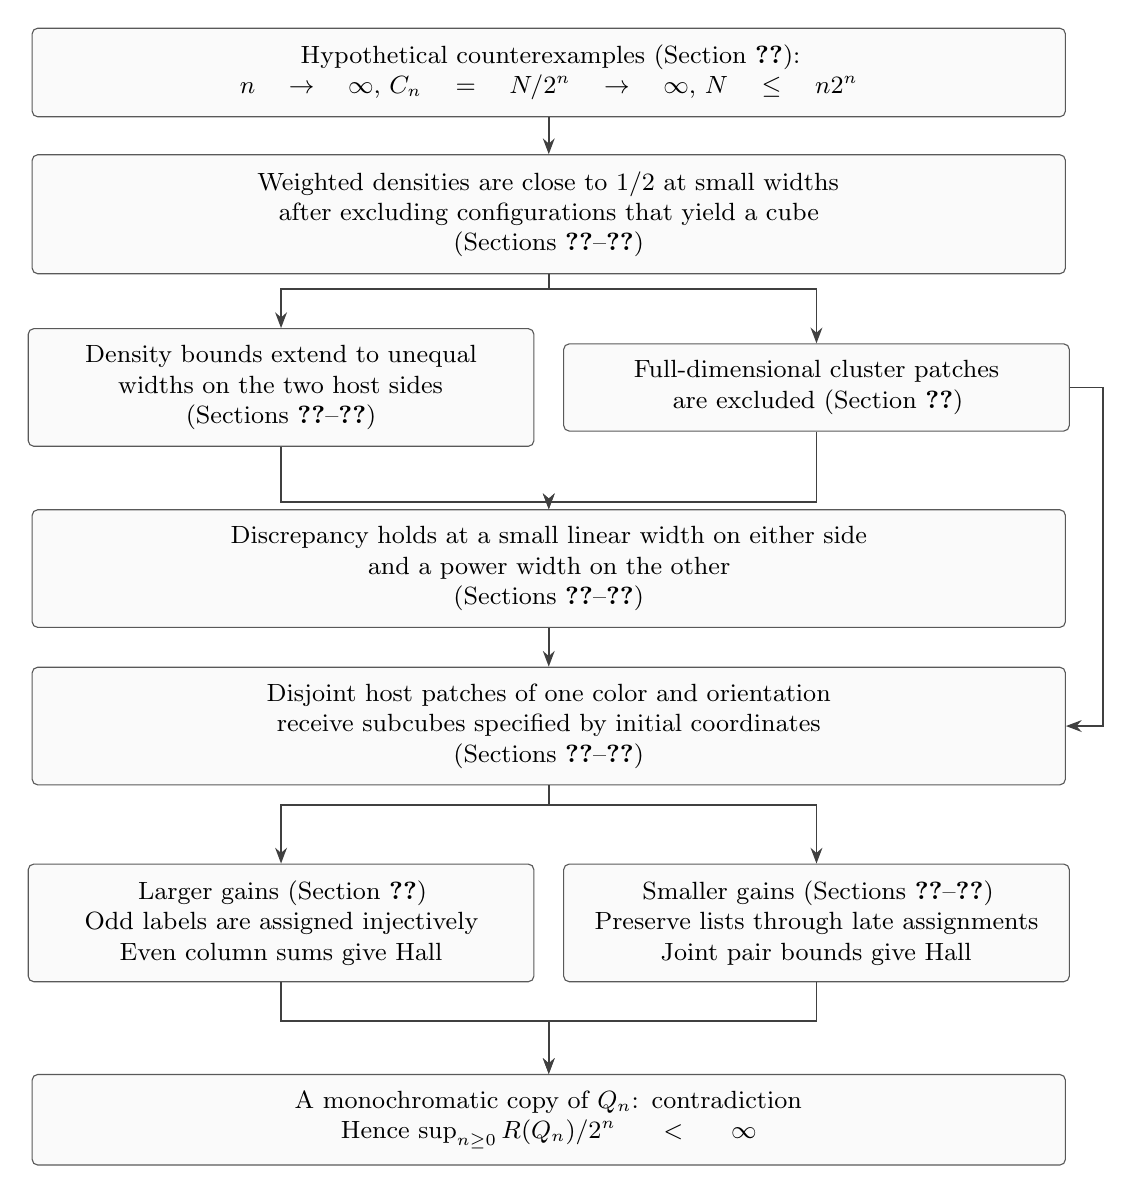
\begin{tikzpicture}[
  x=1cm,y=1cm,
  box/.style={draw=black!65,rounded corners=2pt,fill=black!2,
    align=center,font=\small,inner sep=6pt,text width=6.0cm},
  wide/.style={box,text width=12.7cm},
  arrow/.style={-{Stealth[length=2mm]},line width=.65pt,draw=black!75}
]
\node[wide] (bad) at (0,0)
  {Hypothetical counterexamples (Section~\ref{sec:reduction-and-notation}):\\
   $n\to\infty$, $C_n=N/2^n\to\infty$, $N\le n2^n$};
\node[wide] (small) at (0,-1.8)
  {Weighted densities are close to $1/2$ at small widths\\
   after excluding configurations that yield a cube\\
   (Sections~\ref{sec:bias-versus-purity-at-power-widths}--\ref{sec:a-small-power-key-grid})};
\node[box] (intermediate) at (-3.4,-4.0)
  {Density bounds extend to unequal\\
   widths on the two host sides\\
   (Sections~\ref{sec:asymmetric-pure-patches-under-2}--\ref{sec:intermediate-powers-of-bias})};
\node[box] (clusters) at (3.4,-4.0)
  {Full-dimensional cluster patches\\
   are excluded
   (Section~\ref{sec:full-dimensional-cluster-patches})};
\node[wide] (deep) at (0,-6.3)
  {Discrepancy holds at a small linear width on either side\\
   and a power width on the other\\
   (Sections~\ref{sec:jump-to-large-bias-only-at-linear-budget}--\ref{sec:the-two-deep-orientations-some-estimates})};
\node[wide] (tiling) at (0,-8.3)
  {Disjoint host patches of one color and orientation\\
   receive subcubes specified by initial coordinates\\
   (Sections~\ref{sec:patch-tiling-under-9}--\ref{sec:internal-solver-and-profiles-for-these-tilings})};
\node[box] (high) at (-3.4,-10.8)
  {Larger gains (Section~\ref{sec:high-modes-of-the-tiling})\\
   Odd labels are assigned injectively\\
   Even column sums give Hall};
\node[box] (low) at (3.4,-10.8)
  {Smaller gains (Sections~\ref{sec:low-modes-geometry-and-cell-states}--\ref{sec:late-dynamics-and-its-transfer-problem})\\
   Preserve lists through late assignments\\
   Joint pair bounds give Hall};
\node[wide] (cube) at (0,-13.3)
  {A monochromatic copy of $Q_n$: contradiction\\
   Hence $\sup_{n\ge0}R(Q_n)/2^n<\infty$};
\draw[arrow] (bad) -- (small);
\draw[arrow] (small.south) -- (0,-2.75) -| (intermediate.north);
\draw[arrow] (small.south) -- (0,-2.75) -| (clusters.north);
\draw[arrow] (intermediate.south) |- (0,-5.45) -- (deep.north);
\draw[arrow] (clusters.south) |- (0,-5.45) -- (deep.north);
\draw[arrow] (deep) -- (tiling);
\draw[arrow] (clusters.east) -- ++(.42,0) |- (tiling.east);
\draw[arrow] (tiling.south) -- (0,-9.3) -| (high.north);
\draw[arrow] (tiling.south) -- (0,-9.3) -| (low.north);
\draw[arrow] (high.south) |- (0,-12.05) -- (cube.north);
\draw[arrow] (low.south) |- (0,-12.05) -- (cube.north);
\end{tikzpicture}
\caption{Logical dependencies of the proof. Each reduction is carried out
along the hypothetical counterexample sequence, passing to subsequences
and removing a vanishing fraction of labels where needed. The separate
arrow from cluster exclusion to patch extraction records its second use:
it bounds the measured scales of the remaining cluster patches.
One common color and orientation are fixed before cube allocation.
The final estimates apply to every sequence $C_n\to\infty$, with no
prescribed rate of divergence.}
\label{fig:proof-roadmap}
\end{figure}


\Needspace{24\baselineskip}
\subsection{Terminology}

All constants and exponents are fixed before $n\to\infty$. A fixed
threshold for a small patch scale need not grow with $n$.

\begin{center}
\begin{tabular}{@{}p{.22\linewidth}p{.71\linewidth}@{}}
\toprule
Term or symbol & Meaning \\
\midrule
Position or role & A vertex of the cube being embedded. \\
Label & A vertex of the host graph. \\
$X,Y,N$ & Disjoint host sides, each initially of size $N$; later width
normalizations continue to use this original $N$. \\
$C_n$ & The ratio $N/2^n$, tending to infinity at an unspecified rate. \\
Width of $\mu$ & $\log(N\max_x\mu(x))$, with natural logarithms. \\
Patch and $M_i$ & In the final tiling, a pair of retained host sets of common
size $M_i$, used for a portion of the cube. Earlier patches are specified
by their laws. \\
Raw law & The specified law before the avoidance constraints of the stage
being discussed. \\
Gate & An event indicator included in a probability or likelihood to
restrict it to specified local conditions; it does not normalize the law. \\
Profile & A probability distribution on a finite set of permitted local
choices, chosen to balance expected label masses. \\
\bottomrule
\end{tabular}
\end{center}

\clearpage
\tableofcontents
\clearpage
\section{Reduction and notation}
\label{sec:reduction-and-notation}

We prove Theorem~\ref{thm:main} by contradiction along sequences.
All constants in an asymptotic argument, including exponents unless
explicitly indicated otherwise, are independent of \(n\).

\begin{lemma}[Counterexample sequence]\label{lem:counterexample-sequence}
If \(R(Q_n)/2^n\) is unbounded, there is a sequence of dimensions and
red-blue colorings between disjoint sets \(X,Y\), each of size \(N\),
with no monochromatic \(Q_n\) across the two sides, such that
\[
 n\longrightarrow\infty,\qquad C_n=N/2^n\longrightarrow\infty,\qquad N\le n2^n.
\]
\end{lemma}
\begin{proof}
Each fixed dimension has finite Ramsey number by the finite Ramsey
theorem~\cite{ramsey1930}. Thus an unbounded ratio has a subsequence along
which both the dimensions and the ratios tend to infinity. For each such
\(n\), take a coloring of \(K_{R(Q_n)-1}\) containing no monochromatic
\(Q_n\), and set
\[
N=\min\left\{\left\lfloor\frac{R(Q_n)-1}{2}\right\rfloor,
                 n2^n\right\}.
\]
Choose \(2N\) of its vertices and split them into equal sides. Restriction
to the cross edges cannot create a monochromatic cube. Moreover,
\(N/2^n\to\infty\), since both terms in the defining minimum have ratios
tending to infinity.
\end{proof}

Fix such a sequence for the remainder of the proof. We will contradict its
existence without imposing any rate of growth on \(C_n\).

Write \(A\) and \(B\) for the even and odd vertices of \(Q_n\). We call
these vertices \emph{roles} or \emph{positions}, and call host vertices
\emph{labels}. Usually the embedding sends \(A\) to \(X\) and \(B\) to
\(Y\); we may interchange the host sides. Distances between cube positions
are Hamming distances.

After labels have been discarded, all size and law normalizations still
use the original side size \(N\), unless another normalization is stated.
For a probability law \(\mu\) on either host side, define its \emph{width}
by
\[
 \operatorname{width}(\mu)=\log\bigl(N\max_x\mu(x)\bigr).
\]
Thus the uniform law on a set of \(M\) labels has width \(\log(N/M)\).
All logarithms are natural.

For a color \(G\) and laws \(\mu\) on \(X\), \(\nu\) on \(Y\), put
\[
 d_G(\mu,\nu)=\sum_{x\in X}\sum_{y\in Y}
                  \mu(x)\nu(y)\mathbf 1_{\{xy\in G\}}.
\]
This is the edge density seen by independent draws from the two laws.
A label in an argument of \(d_G\) denotes its point mass. A label
\emph{hits} another label in \(G\) when the two are adjacent in that
color. We leave integer roundoffs in scales and layer counts implicit
when the accompanying asymptotic inequalities have slack.

The tools in Section~\ref{sec:general-conventions-and-probabilistic-tools}
are used throughout. Sections~\ref{sec:bias-versus-purity-at-power-widths}--\ref{sec:a-small-power-key-grid}
establish the initial discrepancy bound~\eqref{eq:source-2};
Sections~\ref{sec:asymmetric-pure-patches-under-2}--\ref{sec:jump-to-large-bias-only-at-linear-budget}
exclude asymmetric purity, intermediate bias, full-dimensional clusters,
and the linear-budget jump.
Section~\ref{sec:the-two-deep-orientations-some-estimates} records the
resulting deep discrepancy and interaction estimates.
Sections~\ref{sec:patch-tiling-under-9}--\ref{sec:high-modes-of-the-tiling}
extract patches, allocate the cube, and exclude the high modes.
Sections~\ref{sec:low-modes-geometry-and-cell-states}--\ref{sec:late-dynamics-and-its-transfer-problem}
handle the bounded and low modes, ending with the two-endpoint Hall
estimate. Figure~\ref{fig:proof-roadmap} shows the dependencies between
these reductions.

\section{General conventions and probabilistic tools}
\label{sec:general-conventions-and-probabilistic-tools}

This section supplies the finite tools used throughout the proof. We first
retain witness families after small removals and balance their expected
label loads. We then prove conditional probability comparisons, a local
construction for choosing centers, and two samplers that assign distinct
labels. Each later application specifies the laws and local tests to which
these tools are applied.

\begin{definition}[Availability]
A witness has specified supports on the current host sides. After a pair
of label removals, it remains a witness if both supports are wholly
retained. A family is \textbf{available} along a sequence if some constant
\(\kappa>0\) has the following property: eventually, after every removal
of at most \(\kappa N\) labels from each side, at least one witness remains.
The witness may be chosen anew for each pair of removals.
\end{definition}

\begin{lemma}[Stabilization and finite menus]\label{lem:stabilization}
For a countable list of existence properties defined by witnesses
intrinsic to their supports, we can pass to a subsequence and discard
\(o(N)\) labels so that each property is either eventually absent or
available. Every fixed earlier availability survives with a smaller fixed
removal tolerance. An available finite union has an available member after
passing to a subsequence. An available menu can be replaced by a finite
menu at each dimension.
\end{lemma}

\begin{proof}
Treat the properties in order. If the current property can be eliminated
by \(o(N)\) additional removals along a subsequence, make those removals
and pass to that subsequence. Otherwise it is available: failure of every
fixed tolerance would let us choose successive dimensions at which
removals of size at most \(N/j\) eliminate the property, producing just
such a subsequence. Diagonalize these nested subsequences, choosing each
term sufficiently far out that the accumulated removals have size
\(o(N)\). For each fixed earlier stage, the later removals eventually use
less than half of its tolerance. Its availability therefore persists with
half that tolerance, while an absence persists under every further removal.

For an available union of \(k\) families with tolerance \(\kappa\), use
\(\kappa/k\) as the removal tolerance for each member. If no member were
available on a subsequence, we could combine their eliminating sets and
eliminate the union within its tolerance. Finally, there are only finitely
many pairs of label subsets at any fixed dimension. For each allowed
removal pair choose one surviving witness. These representatives form a
finite menu with the same availability.
\end{proof}

\begin{lemma}[Balanced mixtures and simultaneous profiles]\label{lem:balanced-profiles}
Let a finite patch menu be available with tolerance \(\kappa>0\), and let
patch \(i\) carry laws \((\mu_i,\nu_i)\) on its two supports. There is a
probability distribution on the menu such that, coordinatewise,
\[
 \mathbb E_i\mu_i,\ \mathbb E_i\nu_i\le K/N
\]
for a constant \(K\).

More generally, let finitely many players have finite action sets and
choose their actions independently according to probability distributions
called \emph{profiles}. Conditional on the realized actions, fix each
player's output-vector rule independently of the profiles. Suppose that,
for every choice of the other players' profiles, a player can meet its
fixed expected-vector upper bounds by a mixture of its actions. Then
there is a profile for every player under which all these bounds hold
simultaneously.
\end{lemma}

\begin{proof}
For the first assertion, assign nonnegative prices to labels on the
disjoint union of the host sides, and let \(P\) be their total. If \(P=0\)
there is nothing to prove. Otherwise, fewer than \(\kappa N\) labels on
either side have price greater than \(2P/(\kappa N)\). Availability gives
a patch avoiding all these labels. Each of its two laws then has expected
price at most \(2P/(\kappa N)\), so its pair-vector has price at most
\(4P/(\kappa N)\). If the convex hull of the pair-vectors contained no
vector bounded coordinatewise by \(4/(\kappa N)\), separation from that
downward-closed region would give nonnegative prices contradicting this
inequality. Thus \(K=4/\kappa\) suffices.

For the second assertion, write \(X_j\) for player \(j\)'s output vector
and \(b_j\) for its prescribed upper bound. With the other profiles
\(p_{-j}\) fixed, its feasible responses form
\[
 \mathcal R_j(p_{-j})
   =\{q_j:\mathbb E_{q_j,p_{-j}}X_j\le b_j\}.
\]
These sets are nonempty by hypothesis, and are closed and convex because
expectation is linear in \(q_j\). Since the action sets are finite and the
output rules are fixed, the expectations are continuous in all profiles;
hence the response correspondence has closed graph. The product of these
correspondences has a fixed point by Kakutani's theorem~\cite{kakutani1941}.
At that point every player's expected-vector bound holds.
\end{proof}

A kernel below may be a \emph{subprobability}, a nonnegative measure of
mass at most one. For example, a row \(p_v\), indexed by a cube role
\(v\), may be set to zero when its local construction is invalid.
Auxiliary experiments may instead use a specified fallback draw to
continue sampling. The final rows on a successful outcome must be
probability measures. If they are supported on the allowed labels and
\(\sum_v p_v(y)\le1\) for each label \(y\), then for every set \(S\) of
roles,
\[
 |S|=\sum_y\sum_{v\in S}p_v(y)
 \le\left|\bigcup_{v\in S}\operatorname{supp}p_v\right|.
\]
Hall's theorem~\cite{hall1935} therefore gives distinct allowed
representatives.

\begin{definition}[Raw experiments, gates, and stage histories]
A \emph{raw experiment} is the specified sampling law before the avoidance
constraints currently under discussion are imposed. A \emph{local gate}
is an event determined by the declared local inputs; retaining the gate
means multiplying by its indicator, rather than conditioning the
reference law on it. A \emph{successful prehistory} is an entering stage
history on which that stage's stated hypotheses hold. Comparisons are
made separately at each such history.
\end{definition}

The next comparisons bound expectations of arbitrary nonnegative tests.
An absolute estimate for the probability of failure would not suffice
when the test itself has very small probability.

\begin{lemma}[Conditional avoidance comparison]\label{lem:conditional-avoidance}
Let \(E_i\) be finitely many bad events with a symmetric neighbor relation
\(\sim\). Suppose that, whenever defined, the probability of \(E_i\)
conditioned on avoidance of any subset of its nonneighbors other than
itself is at most \(p_i\). Independent underlying variables, with events
joined when their variable scopes overlap, satisfy this hypothesis with
\(p_i=\Pr(E_i)\). Assume
\[
 p_i\le x_i\prod_{j\sim i}(1-x_j),\qquad 0\le x_i<1.
\]
Then all the events can be avoided with positive probability. For any set
\(S\) of indices not containing \(i\),
\(\Pr(E_i\mid \bigcap_{j\in S}E_j^c)\le x_i\).

Write \(A_S=\bigcap_{j\in S}E_j^c\). For disjoint index sets \(S,T\) and
any nonnegative random variable \(W\),
\[
 \mathbb E[W\mid A_{S\cup T}]
 \le \prod_{j\in T}(1-x_j)^{-1}\mathbb E[W\mid A_S].
\]
If an additional event \(F\) has conditional probability at most \(p_F\)
under avoidance of any subset of its nonneighbors, then
\[
 \Pr(F\mid A_S)\le
 p_F\prod_{j\in S:\,j\sim F}(1-x_j)^{-1}.
\]
\end{lemma}

\begin{proof}
The local lemma and its conditional induction go back to Erd\H{o}s and
Lov\'asz~\cite[Section~2]{erdos-lovasz1975}. Erd\H{o}s and
Spencer introduced the lopsided nonneighbor condition~\cite[Section~1]{erdos-spencer1991};
see Lu and Sz\'ekely~\cite[Lemma~3]{lu-szekely2007} for the asymmetric
formulation used here.
Here is the induction for the stated hypotheses. Split a conditioning
set into nonneighbors and neighbors of \(E_i\). The numerator is bounded
by \(p_i\) after discarding neighbor-avoidance conditions. By induction,
each neighbor-avoidance condition has conditional probability at least
\(1-x_j\), so the denominator is at least their product. This proves
\(\Pr(E_i\mid A_S)\le x_i\), and simultaneously proves positivity of all
avoidance probabilities. In particular,
\[
 \Pr(A_T\mid A_S)\ge\prod_{j\in T}(1-x_j).
\]
Inserting \(\mathbf1_{A_T}\le1\) in the conditional expectation of
\(W\), then dividing by this lower bound, proves the first comparison.
The same argument for \(F\) removes only its neighbors and uses its own
conditional nonneighbor bound for the remaining numerator.
\end{proof}

For independent underlying variables, removing all avoidance constraints
that touch a specified set of variables makes those variables independent
of the remaining avoidance event. They can then be integrated under their
raw laws. In applications we impose avoidance separately at each entering
history; we do not reweight earlier draws by the probability of later
avoidance.

\begin{lemma}[Scattered moments]\label{lem:scattered-moments}
Let \(Z_v\ge0\), indexed by a finite role set \(U\), be bounded by \(L\)
on a success event. Each role has a near set, including itself, of size at
most \(f|U|\). Suppose that for any sequence of at most \(n\) indices,
each outside the near sets of its predecessors, the joint product
expectation with the success indicator is at most \(K^n\) times the
product of deterministic comparison means \(d_v\), where \(K\ge1\).
Then
\[
 \mathbb E\!\left[\mathbf1_{\rm success}
       \bigl(|U|^{-1}\textstyle\sum_v Z_v\bigr)^n\right]
 \le K^n\bigl(|U|^{-1}\textstyle\sum_v d_v+nfL\bigr)^n.
\]
\end{lemma}

\begin{proof}
Expand the power by drawing \(n\) indices independently and uniformly
from \(U\). Mark a position as removed if its index lies in the near set
of any preceding index. On success each removed factor costs at most
\(L\); the unremoved indices satisfy the joint-comparison hypothesis.
For each removal pattern, apply that comparison, then discard the
separation conditions at the unremoved positions. Sum over the indices
in reverse order. At an unremoved position the factor is
\(|U|^{-1}\sum_v d_v\). At a removed position the necessary proximity
condition permits at most an \(nf\) fraction of indices, so its factor is
at most \(nfL\). Summing over all removal patterns gives the claimed
binomial expansion.
\end{proof}

We may first apply the joint comparison conditional on a successful
prehistory, retaining its indicator, and only afterwards discard
nonlocal restrictions for an upper bound. Typically \(nfL=o(1)\), while
\(K\) and the average of the \(d_v\)'s are bounded. Markov's inequality
at a sufficiently large constant threshold then permits a union over
\(\exp(O(n))\) columns. For \(Z_v=Np_v(y)\), the resulting bound on the
average gives
\[
 \sum_{v\in U}p_v(y)
   =\frac{|U|}{N}\left(|U|^{-1}\sum_{v\in U}Z_v\right)=o(1)
\]
when \(|U|=O(2^n)\), since \(N=C_n2^n\) and \(C_n\to\infty\).
The exceptional probability here includes the success indicator. We also
use this argument with patch-specific sizes.

\begin{lemma}[Gated posterior comparison]\label{lem:gated-posterior}
Fix any earlier information in a reference experiment. Let a candidate
\(z\) have prior law \(\pi\), and let \(F_z(t)\) be the likelihood of data
\(t\) together with a required event. Thus \(F_z\) includes the event
indicator and may have total mass less than one. Set
\[
 m(t)=\int F_z(t)\,d\pi(z).
\]
Use one common reference measure for all data densities; in a finite
space these may simply be masses. If \(Q\) is any reference probability
law on the data fixed by the earlier information and \(\epsilon>0\), then the joint
probability of the required event and
\(\{m(t)<\epsilon Q(t)\}\cup\{m(t)=0\}\) is at most \(\epsilon\).
If also \(F_z(t)\le e^sQ(t)\), the posterior
\(F_z(t)\,d\pi(z)/m(t)\) outside this exception is dominated by
\(e^s\epsilon^{-1}\pi\). Integrating the posterior against the required-event
data measure recovers the prior experiment with its gate retained.
\end{lemma}

\begin{proof}
The data measure with the required event has density \(m\). Its mass on
\(\{m<\epsilon Q\}\) is at most \(\epsilon\int Q=\epsilon\), and its
mass where \(m=0\) is zero. On the complement,
\(F_z/m\le e^s/\epsilon\). Finally, for any nonnegative test \(h\),
\[
 \int m(t)\int h(z,t)\frac{F_z(t)}{m(t)}\,d\pi(z)\,dt
   =\int\!\int h(z,t)F_z(t)\,dt\,d\pi(z),
\]
with the left integrand set to zero where \(m=0\). This is the asserted
cancellation.
\end{proof}

The gate and every selection rule in \(F_z\) must be recomputed as \(z\)
varies. To use this estimate after an assignment, we first compare the
joint law of the required outputs with the reference experiment. Only
then may we remove nonlocal prehistory restrictions, keeping the local
gate inside \(F_z\).

\subsection{Geometric height device}
\label{sec:geometric-height-device}

We next choose centers in Hamming balls while keeping the choices at
nearby sites geometrically compatible. A center has an ID consisting of
its location and level. The construction gives neighboring sites levels
that differ by at most one, and bounds the number of active IDs they can
consult. Its path-maximum rule is related to the admissible-path
construction of Lipschitz percolation~\cite[Sections~4--5]{dirr-dondl-grimmett-holroyd-scheutzow2010}.
Here eligibility may depend on all the sampled center positions, so the
independence needed in the proof comes only after separating those
positions from the later activations.

Let the queried sites form a subset \(S\) of \(Q_d\), where
\(d=\Theta(n)\). A horizontal step may join queried sites at Hamming
distance at most a fixed positive integer \(D\), including a step that
stays at the same site. Prospective center locations range over all of
\(Q_d\). Write \(V\) for the volume of a radius-\(r\) ball in \(Q_d\).
For levels \(0,\ldots,H\), the random experiment has three stages:
\begin{enumerate}[label=(\roman*),leftmargin=*]
\item At each vertex of \(Q_d\) and each level, independently, put a
prospective center with probability \(\lambda/V\), where
\(\lambda=n^{J_0}\) and the fixed constant \(J_0>2\). Write \(P\) for
all these prospective positions.
\item Using \(P\) and any auxiliary information, specify for every
site-level \((v,j)\) an eligible set \(E(v,j)\) of prospective centers in
its same-level \(r\)-ball. The required size is \(|E(v,j)|\ge\lambda/3\).
\item After those choices, activate each prospective center independently
with probability \(n^{b_0}/\lambda\). Write \(A\) for these activation
variables, where \(0<b_0<b<1\).
\end{enumerate}
A site-level is \emph{bad} if its eligible set contains no active center,
or if its same-level \((r+D)\)-ball contains more than \(n^b\) active
centers. We allow either of the following radii:
\begin{itemize}
\item \(r=\Theta(d)\) with \(r\le(1/4+o(1))d\);
\item \(r=\lfloor n^{1-\rho}\rfloor\), for fixed \(0<\rho<1\), with
\(b>b_0+(D+1)\rho\).
\end{itemize}
Choose fixed \(0<\sigma<\zeta<1\), \(0<\theta<1\), and \(a>0\) such that
\[
 b_0>a>\zeta+\sigma+(1-\theta),\qquad b>a+4\sigma.
\]

A space-level path stays in levels \([0,H]\). Its permitted steps are an
upward vertical step from a bad site-level, or a downward step of one
level together with a horizontal step. For a queried site \(v\), restrict
the whole path to spatial distance \(2DH\) from \(v\). Define the
\emph{long height} \(h(v)\) to be the largest \(j\) for which \((v,j)\)
is reachable by such a path from any level-zero start. A rule with a
shorter consultation radius restricts the same paths to the smaller ball.
If the resulting height equals \(H\) or its site-level is bad, the rule
makes no selection.

\begin{lemma}[Local height selection]\label{lem:height-selection}
In this experiment, take
\[
 R_0=\lceil\log^2 n\rceil,\qquad
 R_i=MR_{i-1},\qquad M=\lceil n^\sigma\rceil,
\]
and let \(H=R_h\) be the first scale at least \(n^{1-\zeta}\). Thus
\(H=O(n^{1-\zeta+\sigma})\).
\begin{enumerate}[label=(\roman*),leftmargin=*]
\item Except on an event of probability at most \(\exp(-n^{1+c})\), for
some fixed \(c>0\), whenever all eligible sets have the required sizes,
the long heights lie in \(\{0,\ldots,H-1\}\), their site-levels are good,
and their values differ by at most one on horizontal steps. Computing a
long height uses only bad statuses within spatial distance \(2DH\).
\item At a fixed site, on correct eligible-set sizes throughout its
consultation domain, the probability of positive long height is at most
\(\exp(-n^c)\) for some fixed \(c>0\). This remains true if one specified
prospective center is forced present.
\item If \(\theta>.9\), \(m=n^{\alpha+o(1)}\) for fixed \(\alpha>0\), and
\(\sqrt m\le H\), replacing the consultation radius by
\(D\lfloor\sqrt m\rfloor\) changes the path maximum with probability
\(o(\exp(-2m^{1/5}))\), on the same correct sizes. This estimate also
allows one forced prospective center.
\end{enumerate}
All bounds on correct sizes concern intersection with that event, not
conditioning on it. The local bounds in (ii) and (iii) also hold when,
for each fixed \(P\), one takes the supremum of the conditional activation
probability over fixed legal eligibilities, and only then averages over
\(P\).

At a good chosen height, independent pre-randomized site-level ties can
select a uniform eligible active ID. For fixed \(P,E\) of the required
sizes and a specified present ID \(c\) at level zero,
\[
 \Pr_{A,\,\mathrm{ties}}(h(v)=0\text{ and }c\text{ is selected}\mid P,E)
 \le 3/\lambda.
\]
The long and short rules may use the same ties and invalid-choice
conventions.
\end{lemma}

\begin{proof}
\noindent\textbf{Step 1: the path event to be estimated.}\quad
Use the metric
\[
 \operatorname{dist}((v,j),(v',j'))
   =\max\bigl(|j-j'|,\lceil d_H(v,v')/D\rceil\bigr).
\]
There are a bounded number of scales. Choose
\(1/4\le\eta_h<\cdots<\eta_0\le1/2\) with fixed positive gaps. A
scale-\(i\) failure from a specified point is a path stopped when it first
reaches metric distance \(R_i\), with net rise at least \(-\eta_iR_i\).
We will bound its probability by \(\exp(-n^aR_i^\theta)\), in the uniform
form specified below. The proof first finds many separated short failures inside a long one.
Their center balls may overlap. Removing the shared regions, while
allowing a small loss in the size and crowd thresholds, makes the short
failures depend on disjoint random inputs.

Fix a deterministic domain \(\mathcal D\) of allowed site-level paths and
a deterministic set \(\mathcal C\) of location-levels that may provide
centers. Both eligibility and crowd counts use only \(\mathcal C\).
At scale \(i\), require eligibility
size at least \(s_i\lambda\) and call a crowd bad above \(t_i n^b\), where
\(s_i\) increase strictly within \([1/8,1/4]\) and \(t_i\) increase
strictly within \([1/3,3/4]\), with fixed positive gaps. Let
\(F_i(P,E,A)\) be the scale failure from the specified start in these
domains with these thresholds. With \(\mathcal D,\mathcal C\) fixed, define
\[
 B_i(P)=\sup_E\Pr_A(F_i(P,E,A)\mid P,E),
\]
where eligible sets must have the stated sizes within metric distance
\(R_i\) of the start; the supremum is zero if no such sets exist. This
defines a random variable depending only on the prospective positions.
The induction claim, uniform in the two deterministic domains, is
\begin{equation}
 \mathbb E_P B_i(P)\le\exp(-n^aR_i^\theta).
 \label{eq:source-H}
\end{equation}
The actual thresholds are stronger:
actual legal sets have size at least \(\lambda/3\), and every actual bad
site-level remains bad when the crowd threshold is lowered to
\(t_i n^b\). Hence the same upper bound holds for failures in the original
experiment on correct sizes.

\noindent\textbf{Step 2: the smallest scale.}\quad
A scale-zero failure must contain an up-step. Without one, reaching
distance \(R_0\) requires at least \(R_0\) downward steps and gives net
rise at most \(-R_0\). An up-step identifies a bad site-level in the
metric ball of the start. There are at most
\(\exp(O(R_0\log n))\) possible such points.

For any fixed legal eligible set, a hole has conditional probability at
most \(\exp(-s_0n^{b_0})\). The crowd test does not depend on eligibility.
Unconditionally its count is binomial, with mean at most
\(n^{b_0}O(1)\) in the linear-radius case and
\(n^{b_0}O(n^{D\rho})\) in the sublinear case, by successive Hamming-layer
ratios. The assumed gap below \(b\) gives a binomial upper tail with
polynomial slack. The same union bound is valid after taking the
eligibility supremum: the hole bound is uniform in the eligible set,
and the crowd bound is independent of it. Since \(b_0>a\), these tails
and the count of possible points prove the induction at scale zero.

\noindent\textbf{Step 3: separated child paths and ball intersections.}\quad
Put \(R'=R_{i-1}\). A scale-\(i\) failure contains at least
\(q=\lfloor c'M\rfloor\) starts of scale-\((i-1)\) failures separated
by \(KR'\), with all child paths still inside the parent's metric ball.
Here the child paths temporarily use the parent's bad statuses; \(K\)
is a large fixed constant and \(c'>0\) is sufficiently small.

To see this, take a maximal separated set of child-failure starts. If it
has fewer than \(q\) members, their \(KR'\)-balls cover every such start.
Follow the parent path. Whenever it enters the cover, skip to its last
visit to the currently hit ball, accounting separately for one outgoing
step if necessary. No ball is used twice. These skips are bookkeeping:
each has endpoint displacement, and hence possible upward displacement,
at most \(2KR'\). Outside the cover, partition the path into pieces
stopped on first reaching distance \(R'\), with one unfinished piece per
intervening stretch. Every full piece has rise less than
\(-\eta_{i-1}R'\), since its start is not a child-failure start. The parent
displacement forces at least \(M-O((q+1)K)\) full pieces. Its total rise
is consequently at most
\[
 -\eta_{i-1}MR'+O((q+1)KR'),
\]
which is less than \(-\eta_iMR'\) when \(c'\) is small relative to the
gap \(\eta_{i-1}-\eta_i\). This contradicts the parent failure.

There are at most \(\exp(O(qR_i\log n))\) choices of these starts.
A child's center domain has levels within \(R'\) of its start and spatial
radius at most \(r+DR'+D\). For two separated children, either their
level intervals are disjoint or their spatial centers have distance
\(s\) at least a large multiple of \(R'\). At each common level, the
intersection of their enlarged balls has volume
\(V\exp(-\Omega(R'))\).

For this last estimate, a uniform point of one enlarged ball lies within
\(s/10\) of its outer layer except with probability
\(\exp(-\Omega(s))\), by the binomial-layer ratios. If it also lies in
the other ball, it must then flip at least \(.44s\) of the \(s\)
coordinates on which the centers differ. The enlarged radius is at most
\((1/4+o(1))d\), so this is a hypergeometric upper tail of probability
\(\exp(-\Omega(s))\). For sublinear radius, the enlarged ball has
radius at most \(n^{1-c''}\) for some fixed \(c''>0\); layer ratios and
a subset union bound for the differing coordinates improve both
exponents to \(\Omega(s\log n)\). Enlarging the original ball costs a
factor \(\exp(O(R'))\), or \(\exp(O(R'\log n))\) in the sublinear case.
Taking \(K\) large makes the intersection bound valid relative to \(V\)
in either case.

\noindent\textbf{Step 4: removing shared centers.}\quad
For a fixed configuration of child starts, delete every pairwise overlap
from each child center domain. The remaining regions are deterministic
and disjoint. Choose a small fixed \(\varepsilon>0\) below all the gaps
\(s_i-s_{i-1}\) and \(t_i-t_{i-1}\). Except on an event of probability
\(\exp(-\Omega(n^bR'/q))\) per pair and level, an overlap contains at most
\(\varepsilon\lambda/q\) prospective centers and
\(\varepsilon n^b/q\) active centers. Indeed their means are at most
\(\lambda e^{-\Omega(R')}\) and \(n^{b_0}e^{-\Omega(R')}\), respectively,
so the claimed estimates follow from binomial upper tails.

If none of these count exceptions occurs, each child loses at most
\(\varepsilon\lambda\) eligible centers and \(\varepsilon n^b\) active
centers. Its eligible sets still have size at least
\(s_{i-1}\lambda\). A hole stays a hole, while a crowd above \(t_i n^b\)
remains above \(t_{i-1}n^b\). Thus all the child failures transfer to the
private regions with the child thresholds.

The probability calculation must not condition on successful overlap
counts. Let \(C\) be the event that the chosen child configuration occurs,
let \(B_{\rm pos},B_{\rm act}\) be the prospective and active overlap
exceptions, and let \(P_\ell\) be the positions in the private region of
child \(\ell\). For every fixed legal eligibility assignment \(E\),
\[
 \begin{aligned}
 \Pr_A(C\mid P,E)
 &\le\mathbf1_{B_{\rm pos}}+\Pr_A(B_{\rm act}\mid P)
          +\prod_\ell b_\ell(P_\ell),\\
 b_\ell(P_\ell)
 &=\sup_{E_\ell}\Pr_A(\text{private child failure}\mid P_\ell,E_\ell).
 \end{aligned}
\]
The transferred events depend on disjoint activations once \(P,E\) are
fixed. Their probabilities are bounded by the displayed private
suprema, even if \(E\) used positions outside those regions. After
paying for the overlap exceptions we have discarded their complements,
so no conditioning remains to destroy independence. The inequality is
uniform in \(E\); taking its supremum and averaging \(P\) factors the
last product, because the \(P_\ell\)'s are independent. Induction bounds
the product of their expectations by \(\exp(-q n^a(R')^\theta)\).

The exponent exceeds both the logarithm of the configuration count and
the desired parent exponent. In fact, using \(R_i=MR'\), \(R'\le n\),
and \(q\asymp M\),
\[
 \frac{n^a(R')^\theta}{R_i\log n}
 \ge\frac{n^{a-\sigma-(1-\theta)+o(1)}}{\log n}\longrightarrow\infty,
 \qquad \frac{q}{M^\theta}\longrightarrow\infty.
\]
The ratio of an overlap-error exponent to the child exponent is at least
\(\Omega(n^{b-a-2\sigma}(R')^{1-\theta})\), which also tends to infinity
because \(b>a+4\sigma\). The number of pair-level exceptions is
polynomial. The union over configurations therefore proves
\eqref{eq:source-H} and the position-averaged induction claim.

If one prospective center is forced present, erase its location-level
from the deterministic center domain. The remaining positions have their
original independent laws. Each eligible set and crowd loses at most one
center, and
\(\lambda/3-1\ge s_i\lambda\), \(n^b-1\ge t_i n^b\) for large \(n\).
Holes persist. Every original bad-path witness therefore remains a
failure at the relaxed thresholds, uniformly in the erased center's
activation. The same induction applies.

\noindent\textbf{Step 5: heights and local approximations.}\quad
At the top scale,
\(n^aH^\theta\ge n^{a+(1-\zeta)\theta}\), whose exponent is greater
than one. Thus \eqref{eq:source-H} permits a union over all sites with
error \(\exp(-n^{1+c})\). A path from level zero that first displaces by
\(H\) would be a scale-\(h\) failure, since its endpoint still has
nonnegative level. Outside the exceptional event no such path exists.
The spatially unrestricted path maximum is therefore below \(H\), and
all paths relevant to a queried maximum lie in its \(2DH\) consultation
tube. A maximizing site-level is good, since otherwise the path could
extend upward. If neighboring maxima differed by more than one, a
downward horizontal step from the higher one would contradict maximality
at the lower site. This proves (i).

For a fixed query, classify paths reaching it by their maximum metric
displacement from their level-zero start. Below \(R_0\), positive height
requires an up-step at one of \(\exp(O(R_0\log n))\) possible points,
so Step 2 applies. For displacements in \([R_i,R_{i+1})\), the first
prefix reaching distance \(R_i\) is a scale-\(i\) failure. There are at
most \(\exp(O(R_{i+1}\log n))\) possible starts near the query. Hence
these paths have total probability at most
\[
 \sum_{i<h}\exp\bigl(O(R_{i+1}\log n)-n^aR_i^\theta\bigr).
\]
Displacements at least \(H\) contribute at most
\(\exp(O(n)-n^aH^\theta)\). The exponent comparisons in Step 4 show
that the sum, together with the base-scale contribution, is at most
\(\exp(-n^c)\). All arguments hold in deterministic restricted path
domains and for position-averaged eligibility suprema. This proves (ii)
with the stated local and forced-center uniformity.

A path reaching the query but leaving its
\(D\lfloor\sqrt m\rfloor\)-tube has displacement from its start at
least \(\sqrt m/3\). Only scales with
\(R_i\ge\sqrt m/(3M)\), or a top-scale failure, need be counted. The
previous sum now has exponent much larger than \(m^{1/5}\), since
\[
 \frac{n^a(\sqrt m/M)^\theta}{m^{1/5}}
  =n^{a-\sigma\theta+\alpha(\theta/2-1/5)+o(1)}\longrightarrow\infty.
\]
Here \(a>\sigma+(1-\theta)>\sigma\theta\) and \(\theta>.9\).
This proves (iii).

Finally, ignore the height and crowd requirements when bounding the
probability of selecting a specified level-zero ID. For fixed \(P,E\),
independent activation and a uniform tie give each member of \(E(v,0)\)
the same probability of selection, at most \(1/|E(v,0)|\le3/\lambda\).
Reinstating the requirements only decreases the joint probability.
Couple the long and short constructions with the same positions,
activations, eligibilities and ties. Whenever their path maxima agree,
the selected ID and its validity agree as well, as required when a short
rule is used inside a hypothetical-candidate calculation.
\end{proof}

\subsection{Near-product injections}
\label{sec:near-product-injections}

The two samplers below use finite row sets and finite output spaces. Row
\(i\) has a full output \(o\in\Omega_i\), with a specified label
coordinate in a common finite label set. Write \(\widehat p_i(o)\) for
its full-output law and \(p_i(y)\) for the label marginal. When there is
no side data these are the same law. An assignment is injective when its
label coordinates are distinct. A pointwise upper bound for prescribed
outputs can be summed against any nonnegative function of those outputs;
this is the form of comparison used later.

Preserving individual marginals while choosing distinct representatives is
an established feature of bipartite dependent rounding; see Gandhi,
Khuller, Parthasarathy and Srinivasan~\cite[Properties~(P1)--(P3)]{gandhi-khuller-parthasarathy-srinivasan2006}.
Their negative-correlation guarantee concerns edges incident to a common
vertex. The next lemma additionally controls prescribed outputs on
arbitrary distinct rows, with a relative error even when their
probabilities are very small.

\begin{lemma}[Calibrated near-product injections]\label{lem:near-product-injection}
Let a finite set of rows have laws on \(d\) labels, with
\(p_i(y)\le d^{-.95}\) and \(\sum_i p_i(y)\le .4\) for every label
\(y\). For sufficiently large \(d\), there is an injective random
assignment \((O_i)_i\) with exact individual full-output marginals
\(\widehat p_i\) and, for every set \(J\) of \(l\le d^{.025}\) queried
rows and prescribed outputs \((o_i)_{i\in J}\),
\begin{equation}
 \Pr(O_i=o_i\text{ for all }i\in J)
 \le \exp(d^{-.04}l)\prod_{i\in J}\widehat p_i(o_i).
 \label{eq:source-17}
\end{equation}
Targets with repeated labels have probability zero. After sampling the
labels, side data can be drawn independently from their conditional laws
given those labels. We use this sampler for assignments within small bins.
\end{lemma}

\begin{proof}
It suffices to construct the labels: the independent conditional draws
then give both assertions for full outputs.

\noindent\textbf{Step 1: complete the columns and order the rows.}\quad
First allow label atoms \(O(d^{-.95})\) and column sums at most \(1/2\).
If there are \(m\) real rows, then \(m\le d/2\). Put
\(t=\lceil2d/3\rceil\) and write \(c_y=\sum_{i=1}^m p_i(y)\).
Add \(t-m\) identical dummy rows with law
\[
 p_{\rm dum}(y)=\frac{t/d-c_y}{t-m}.
\]
The numerator is nonnegative and sums to \(t-m\), so this is a probability
law. Its atoms are \(O(1/d)\), and every completed column sums to \(t/d\).

Choose an order of the \(t\) rows, then number them in that order, such
that every column prefix satisfies
\[
 \sum_{k<j}p_k(y)=s_j+O(d^{-1/8}),\qquad s_j=(j-1)/d.
\]
A uniform random order has this property with positive probability.
Indeed the expectation is \(s_j\), and exposure without replacement has
martingale increments bounded by the column atom range. Bounded-difference
concentration~\cite{hoeffding1963,azuma1967}, followed by a union over
\(j,y\), gives the asserted error. Fix one such order.

\noindent\textbf{Step 2: track the mass already used.}\quad
At step \(j\), sample row \(j\)'s law conditional on its label still
being free. For each row \(a\), let
\[
 D_j^a=\sum_{k<j}p_a(Y_k),\qquad
 e_j=\max_{a,\,k\le j}|D_k^a-s_k|.
\]
Thus \(D_j^a\) is the mass that row \(a\) assigns to labels used before
step \(j\). Stop at the first \(e_j>1/20\); any undefined continuation
after a stop may be declared a failure. We claim that, with probability
\(1-\exp(-d^{\Omega(1)})\), there is no stop and
\(D_j^a=s_j\pm d^{-.1}\) for all \(a,j\).

Before stopping, all sampling denominators are bounded away from zero.
Conditional on the first \(j-1\) draws, the drift of \(D_j^a\) is
\[
 \mathbb E[D_{j+1}^a-D_j^a\mid Y_1,\ldots,Y_{j-1}]
  =\sum_{y\ \mathrm{free}}\frac{p_a(y)p_j(y)}{1-D_j^j}.
\]
Its martingale increments are \(O(d^{-.95})\). Bounded-increment
concentration gives cumulative errors \(O(d^{-1/8})\), simultaneously
for all rows and times, outside an event of probability
\(\exp(-d^{\Omega(1)})\).

When summing the drifts through step \(b-1\), replacing \(1-D_j^j\) by
\(1-s_j\) costs at most
\[
 O\left(\sum_y p_a(y)\sum_{j<b}e_jp_j(y)\right)
   =O\left(d^{-1/8}+d^{-1}\sum_{j<b}e_j\right).
\]
For the equality, use summation by parts on the column-prefix error
against the bounded nondecreasing sequence \(e_j\). A second summation
by parts replaces \(p_j(y)\) by \(1/d\) in the remaining drift sum:
the sequence \(\mathbf1_{\{y\ \mathrm{free\ before}\ j\}}/(1-s_j)\)
has bounded variation. The resulting sum is
\[
 d^{-1}\sum_{j<b}\frac{1-D_j^a}{1-s_j}+O(d^{-1/8}).
\]
Subtracting \(s_b\) now gives, even at a potential stopping index,
\[
 e_b\le Kd^{-1/8}+\frac Kd\sum_{j<b}e_j.
\]
Iteration bounds \(e_b\) by \(O(d^{-1/8})\). This is smaller than both
\(1/20\) and \(d^{-.1}\) for large \(d\), proving the claim. Call this
successful tracking event \(G\), and condition the sampler on \(G\).

\noindent\textbf{Step 3: compare specified targets multiplicatively.}\quad
Fix \(l\) distinct positive-probability target labels \(y_i\) on queried
rows. Define a second sampler that forces \(Y_i=y_i\) at each queried
step and, at every ordinary step, excludes all target labels whose
queried steps are still pending. On a path realizing the targets and
satisfying \(G\), the likelihood of the original unconditioned sampler
divided by that of the forcing sampler is the product of
\[
 \frac{p_i(y_i)}{1-D_i^i}\quad(i\text{ queried}),\qquad
 1-\frac{\sum_{i>j,\ i\ \mathrm{queried}}p_j(y_i)}{1-D_j^j}
       \quad(j\text{ ordinary}).
\]
After extracting \(\prod_i p_i(y_i)\), the target-step denominators and
the ordinary-step factors cancel to small relative error. For each target,
the prefix estimate and summation by parts give
\[
 \sum_{j<i}\frac{p_j(y_i)}{1-s_j}
       =-\log(1-s_i)+O(d^{-1/8}).
\]
Tracking permits replacement of \(s_j\) by \(D_j^j\) at error
\(O(d^{-.1})\); omitting queried steps costs \(O(l d^{-.95})\) per
target. Thus the linear terms in the ordinary-step logarithms cancel
\(-\log(1-D_i^i)\). The quadratic terms have total size
\(O(l^2d^{-.95})\), because each subtracted fraction is
\(O(l d^{-.95})\) and their sum is \(O(l)\). The total log-error per
target is \(O(d^{-.1}+l d^{-.95})\).

Integrating this ratio under the forcing law, and dividing by
\(\Pr(G)=1-\exp(-d^{\Omega(1)})\), gives the joint upper comparison
\(\exp(O(d^{-.09}l))\prod_i p_i(y_i)\). For a single target the same
ratio also gives a lower comparison \((1-O(d^{-.09}))p_i(y_i)\): the
forcing sampler itself tracks with exponentially small failure
probability. Indeed, before a constant-error stop, excluding the one
pending label changes a step's distribution in total variation by
\(O(p_j(y_i))\). Since the tracked increment is \(O(d^{-.95})\), the
cumulative drift change is
\(O(d^{-.95}\sum_jp_j(y_i))=O(d^{-.95})\); the forced step contributes
another \(O(d^{-.95})\). The proof of Step 2 therefore still applies.
The target mass was extracted before this tracking exception was bounded;
no absolute error is divided by a tiny atom.

\noindent\textbf{Step 4: calibrate the individual marginals exactly.}\quad
Return to the original \(.4\) column bound. For arbitrary real prices
\(c_i(y)\) on the real row-label pairs, put
\(\bar c_i=\sum_y p_i(y)c_i(y)\) and \(\delta=d^{-.05}\). Perturb row
\(i\) by multiplying its probabilities by
\(1+\delta\operatorname{sign}(c_i(y)-\bar c_i)\), then normalize.
Writing \(p'_i\) for the result, its gain in centered expected price is
\[
 \begin{aligned}
 \sum_y p'_i(y)(c_i(y)-\bar c_i)
 &=\frac{\delta\sum_y p_i(y)|c_i(y)-\bar c_i|}
        {1+\delta\sum_y p_i(y)\operatorname{sign}(c_i(y)-\bar c_i)}
 \\
 &\ge\tfrac12\delta\sum_y p_i(y)|c_i(y)-\bar c_i|.
 \end{aligned}
\]
The perturbed rows satisfy the relaxed hypotheses of Step 1. The
tracking sampler's two-sided singleton error is \(O(d^{-.09})\) relative
to \(p'_i\), so its error in this centered price is at most
\(O(d^{-.09})\sum_y p_i(y)|c_i(y)-\bar c_i|\), smaller than the gain.
Its joint upper bound, measured against the \emph{original} inputs, costs
\(\exp(O(d^{-.05}l+d^{-.09}l))\), which fits
\eqref{eq:source-17} for large \(d\).

Let \(\mathcal C\) be the set of all laws on injections of the real rows
satisfying the joint upper inequalities relative to those original
inputs. These are linear inequalities on a finite probability simplex,
so \(\mathcal C\) is compact and convex. Every price-dependent
construction just made belongs to this same set, and its marginal vector
has price at least that of the original marginal vector. If the original
vector were outside the marginal image of \(\mathcal C\), a separating
linear functional would contradict that property. It therefore belongs
to the image, giving exact marginals while preserving all joint bounds.
\end{proof}

\subsection{Clock lemma}
\label{sec:clock-lemma}

The next sampler also enforces local restrictions on full outputs. It
gives a joint upper comparison with the product law, without the exact
marginals of Lemma~\ref{lem:near-product-injection}. We retain the finite
row and full-output spaces, and the notation \(\widehat p_a,p_a\), from
the preceding subsection. A predicate's \emph{scope} is the set of rows
whose full outputs it reads.

\begin{lemma}[Clock sampling]\label{lem:clock-sampling}
Let there be \(g\) labels, with \(\log g=O(n)\), and finitely many
probability rows \(\widehat p_a\). For each fixed \(B\ge1\), there are
sufficiently large constants \(A_*,P_*\) and a small absolute constant
\(\theta_0>0\) with the following property. Suppose
\[
 \sum_a p_a(y)\le\theta_0,\qquad p_a(y)\le n^{-A_*}
\]
for every label and row. Let a finite list of failure predicates have
probability at most \(n^{-P_*}\) under independent row outputs. Assume
each predicate reads at most \(n^B\) rows and each row belongs to at most
\(n^B\) predicate scopes. Then there is a random assignment with distinct
labels avoiding all predicates, such that for every set \(J\) of at most
\(n^B\) queried rows,
\[
 \Pr(O_a=o_a\text{ for all }a\in J)
       \le(1+o(1))\prod_{a\in J}\widehat p_a(o_a).
\]
The error is uniform over the rows and targets for fixed \(B\), the chosen
constants, and a fixed bound in \(\log g=O(n)\). Noninjective targets
have probability zero. Unneeded predicates and an empty assignment may
be ignored.
\end{lemma}

\begin{proof}
Choose \(K_0\) sufficiently large in terms of \(B\), then choose
\(A_*,P_*\) sufficiently large in terms of \(K_0,B\). We first construct
a greedy matching from independent edge clocks and use finite backward
explorations to detect failures. The proof gives two estimates: a joint
product bound for prescribed outputs, and a small total probability for
bad exploration outcomes involving any fixed row or label. The first
controls the raw matching law. The second lets
Lemma~\ref{lem:conditional-avoidance} enforce a match at every real row
and avoidance of every predicate, at a multiplicative cost \(1+o(1)\)
on the queried outputs.

\noindent\textbf{Step 1: trim rare outputs and complete the columns.}\quad
For each row \(a\) and incident failure predicate \(F\), discard outputs
\(o\) for which
\[
 \Pr(F\mid O_a=o)>n^{-P_*/2}
\]
under the product law. Markov's inequality bounds the discarded mass
for each predicate by \(n^{-P_*/2}\), so the total loss per row is at
most \(\varepsilon=n^{B-P_*/2}\). Renormalize the retained laws. A test
or query involves at most \(n^B\) rows, so this changes its probability
by at most \((1-\varepsilon)^{-n^B}=1+o(1)\). Under the new laws, every
predicate has probability at most \(n^{-P_*/3}\), both unconditionally
and after any one row in its scope is pinned to a retained output. We
continue to denote these laws by \(\widehat p_a,p_a\).

Put \(\theta=\lceil10^{-6}g\rceil/g\), and take
\(\theta_0=10^{-8}\), for example. If there are \(m\) real rows and
\(c_y=\sum_a p_a(y)\), add \(\theta g-m\) identical dummy rows with
law \((\theta-c_y)/(\theta g-m)\). This is a probability law because
its numerator sums to the denominator. The denominator is a positive
integer of order \(g\), even after the small trimming loss. Every
completed column sums to \(\theta\), and the dummy atoms are \(O(1/g)\).
The nonempty case has \(g\ge n^{A_*}\), since an original real row is a
probability law with atoms at most \(n^{-A_*}\). Thus the largest edge
rate in the completed row-label graph is
\(\lambda_*=O(n^{-A_*})\).

\noindent\textbf{Step 2: matching and its backward explorations.}\quad
Run an independent Poisson process of rate \(p_a(y)\) on every positive
row-label edge \((a,y)\). Each arrival has an independent mark drawn
from the conditional law of the full output given label \(y\). Through
time \(T_0=K_0\log n\), greedily match an arriving edge if both endpoints
are free. Only its first arrival can matter: if that arrival is rejected,
an endpoint is already matched and never becomes free again.

There are two types of tests. A predicate test fails if all rows in its
scope are matched and their outputs violate the predicate. A real
singleton-row test fails if that row is unmatched. For each test we also
forbid an excessively large exploration of the clocks needed to determine
its outcome.

Start that exploration with the scope rows as roots, each requesting its
matching history through time \(T_0\). An endpoint's requested horizon
is the latest time up to which its status is needed. Process the pending
endpoint with largest horizon. In a fixed order, inspect its incident
edges for first arrivals by that horizon, reusing information already
revealed. A hit at time \(t\) requests the other endpoint through a time
strictly before \(t\); retain the largest request if it is requested
again. Horizons are processed in decreasing order, so a processed
endpoint can never receive a larger request. These inspections determine
the matching decisions at the roots by backward closure through all
earlier events they require.

The active endpoints are the roots and every endpoint reached by a hit,
including pending and processed endpoints. Stop with a \emph{giant}
failure as soon as their number reaches \(L=\lceil n^{.1K_0}\rceil\).
Register the endpoint of the last hit before stopping. Consequently every
inspected hit always has both endpoints active, even on a giant leaf.

\noindent\textbf{Step 3: exploration leaves and nonneighbor conditioning.}\quad
Eventually we discretize first-arrival times with a sufficiently fine
finite mesh and a fixed tie order. A leaf of an exploration then specifies
a product rectangle in the independent edge data. A hit pins an arrival
bin and mark on an edge whose two endpoints are active. A negative
inspection requires absence up to a specified cutoff on an edge with at
least one active endpoint. Every realization in this rectangle follows
the same inspections and reaches the same leaf.

Use the individual bad leaves as forbidden events, joining two leaves
when their active endpoint sets intersect. Leaves with disjoint active
sets can share an inspected edge only if both require absence on it.
To force a positive-probability leaf, condition its edges separately. On
absence edges couple the conditional first time to be no earlier than
the old time; on hit edges fix the required data; leave other edges
unchanged. Every already occurring nonneighbor leaf still occurs. This
holds simultaneously for any collection of nonneighbors, even if they
overlap with one another. If \(A\) is avoidance of such a collection
and \(E\) is the forced leaf, the coupling gives
\(\Pr(A\mid E)\le\Pr(A)\), hence
\(\Pr(E\mid A)\le\Pr(E)\) whenever defined.

It remains to show, uniformly in an endpoint \(u\), that
\[
 \sum_{\substack{E\ \mathrm{bad\ leaf}:\ u\ \mathrm{active\ in}\ E}}
       \Pr(E)\le n^{-.6K_0}.
\]
Equivalently, sum over tests the probability that the test has a bad
outcome and its exploration reaches \(u\). We prove this in continuous
time before choosing the mesh.

\noindent\textbf{Step 4: inserted paths bound the incidence sum.}\quad
Reaching \(u\) from a test's roots requires a path of time-decreasing
arrivals from one of its root rows to \(u\). Such a certificate uses
distinct edges, since the exploration inspects first arrivals; the empty
path is allowed. For a fixed edge path, count its possible distinguished
arrival tuples. Poisson insertion expresses their expected count,
with a specified bad outcome, as the integral of the product of edge
rates over ordered times in \([0,T_0]\), multiplied by the bad-outcome
probability in an ordinary realization with those arrivals inserted.
This identity follows directly by summing over the Poisson counts and
distinguishing one of their uniform-time points on each edge. Inserted
marks may be fixed anywhere in their support for uniform estimates.

To sum certificates, reverse them from \(u\) and allow all walks. Total
outgoing rates alternate between \(1\) at a row and \(\theta\) at a
label. The integrated rate sum for a start at a row is
\[
 \sum_{j\ge0}\theta^{\lfloor j/2\rfloor}\frac{T_0^j}{j!}
 =\cosh(\sqrt\theta T_0)+\theta^{-1/2}\sinh(\sqrt\theta T_0)
 =O(e^{\sqrt\theta T_0}/\sqrt\theta).
\]
Starting at a label only decreases this upper bound. Each root row
belongs to at most \(n^B+1\) tests. Lengths above
\(K_0^2\log n\) contribute less than \(n^{-K_0^2}\) before this
incidence factor, by the factorial tail of the series.

For shorter paths, first dispose of those meeting two distinct rows of
the same test, bounding the bad-outcome probability simply by one. Choose
their two positions on the path and a test incident to the earlier row.
In the normalized reversed walk, a subsequent label-to-row transition
enters that test's scope with probability at most
\(n^B\lambda_*/\theta\). Their total contribution is therefore at most
\[
 O(e^{\sqrt\theta T_0}/\sqrt\theta)(1+\log n)^{O(1)}
       (n^B+1)n^B\lambda_*/\theta.
\]
The remaining short insertions meet at most one row of the test. We now
bound bad outcomes uniformly under each such insertion.

\noindent\textbf{Step 5: the exploration rarely becomes giant.}\quad
Include the endpoints of all inserted arrivals as extra full-horizon
roots. Every reached endpoint is connected to one of these roots by
ordinary arrivals: take the part of its reaching path after the last
inserted hit. There are at most \(n^B+O(\log n)\) roots.

During largest-horizon processing, an edge from the current endpoint to
an unprocessed endpoint is fresh: neither of its endpoints could have
inspected it earlier. Superpose the fresh arrivals and, when necessary,
independent extra arrivals to reach total rate \(1\) at row endpoints
and \(\theta\) at label endpoints. They are dominated by a two-type
branching forest. A node with horizon \(t\) has Poisson children of the
opposite type at times in \([0,t]\), each child inheriting its arrival
time as horizon. To handle repeated requests for a graph endpoint,
attach its sole processing to the node making its highest request;
its offspring have not yet been generated. Unused tree nodes can be
filled with independent subtrees. This deferred construction dominates
the active endpoint count by the forest's total progeny.

For \(\delta=n^{-.01K_0}\), let \(H_{\rm row}(t)\) and
\(H_{\rm label}(t)\) be the exponential moments of single-root progeny,
including the root. They satisfy
\[
 \begin{aligned}
 H_{\rm row}(t)&=\exp\left(\delta+
                    \int_0^t(H_{\rm label}(s)-1)\,ds\right),\\
 H_{\rm label}(t)&=\exp\left(\delta+
                    \theta\int_0^t(H_{\rm row}(s)-1)\,ds\right).
 \end{aligned}
\]
Induction on truncated generations bounds their excesses above one by
\(4\delta e^{2\sqrt\theta t}/\sqrt\theta\) and
\(4\delta e^{2\sqrt\theta t}\), respectively. Substitution proves
these bounds using \(e^x-1\le2x\) for the resulting small positive
exponents. With \(R\le n^B+O(\log n)\) roots, exponential Markov gives
\[
 \Pr(\text{giant})\le
 \exp\left(-\delta L+
      O(R\delta e^{2\sqrt\theta T_0}/\sqrt\theta)\right).
\]
Here \(\delta L\ge n^{.09K_0}\), while the second term is
\(O(n^{B-(.01-2\sqrt\theta)K_0})\). Choosing
\((.1-2\sqrt\theta)K_0>B\) makes this tail superpolynomially small,
uniformly in the fixed short insertion.

\noindent\textbf{Step 6: track the free mass in a background process.}\quad
Fix a prescription removing at most \(2n^B\) endpoints and inserting
\(O(\log n)\) arrivals between the remaining endpoints. In the resulting
background matching define, even for original endpoints that were removed,
\[
 X_a(t)=\sum_{y\ \mathrm{free\ in\ background}}p_a(y),\qquad
 R_y(t)=\sum_{a\ \mathrm{free\ in\ background}}p_a(y).
\]
These are the available label mass of a row and the available row mass
at a label. The deterministic comparison functions solve
\[
 z'=-qz,\qquad q'=-\theta zq,\qquad z(0)=q(0)=1.
\]
In particular \(q=1-\theta+\theta z\) and \(0<q,z\le1\). We claim,
with error probability at most \(\exp(-n^{A_*/3})\), that throughout
\([0,T_0]\), uniformly over original endpoints,
\[
 X_a(t)=q(t)+o(n^{-3B}),\qquad
 R_y(t)=\theta z(t)+o(n^{-3B}).
\]
The estimate is uniform for each fixed removal and insertion prescription;
we do not take a union over all such prescriptions.

A free label \(y\) is matched at ordinary rate \(R_y\), and a free row
\(a\) at rate \(X_a\). Hence the ordinary drifts of these masses are
\(-\sum_{y\ \mathrm{free}}p_a(y)R_y\) and
\(-\sum_{a\ \mathrm{free}}p_a(y)X_a\). If \(E(t)\) is the maximum of
the claimed approximation errors, each drift differs from its ODE drift
by at most \(2E(t)\). Removals cause initial error
\(O(n^B\lambda_*)\), and inserted matches cause total jumps
\(O(\log n\,\lambda_*)\).

The drift-compensated ordinary-jump martingales have jumps at most
\(\lambda_*\) and predictable variance at most \(T_0\lambda_*\).
Their running absolute maxima exceed \(n^{-A_*/4}\) with probability
at most \(\exp(-n^{A_*/2-o(1)})\) per endpoint. For completeness,
compensating \(e^{vM_t}\) costs log-rate at most \(v^2\) times the
variance rate when \(|v|\lambda_*\) is small; this follows from the
exponential series for each jump. Use both signs of
\(v=n^{-A_*/4}/(2T_0\lambda_*)\) and stop at the first crossing. This
is the bounded-jump exponential estimate used here; compare~\cite{freedman1975}.
A union over \(O(g)\) endpoints is permitted by \(\log g=O(n)\).
Finally drift iteration yields
\[
 E(t)\le
 \left[O((n^B+\log n)\lambda_*)+n^{-A_*/4}\right]e^{2T_0}
 \le n^{-A_*/4+2K_0+o(1)}.
\]
Taking \(A_*/4>2K_0+3B\), with slack, proves the claim and its stated
exception probability.

\noindent\textbf{Step 7: ordinary target matches have a product upper bound.}\quad
Fix \(k\le n^B\) full-output targets with distinct labels, also allowing
any fixed short insertion from Step 4. Count tuples of ordinary arrivals
that realize all the target matches. Insert their distinguished arrivals
at candidate times \(t_1,\ldots,t_k\). Their intensities factor out the
entire product \(\prod_a\widehat p_a(o_a)\), including all prescribed
marks, before any probability estimate is made.

If these are the target matches, none of their endpoints ever matches
to an outside endpoint. The outside process therefore agrees exactly
with the background obtained by removing the queried rows and target
labels, keeping the fixed inserted arrivals between remaining endpoints.
Given this background, an ordinary arrival from a target endpoint to a
free outside endpoint is forbidden before its candidate matching time.
These are disjoint clocks independent of the background. Ignoring other
necessary conditions gives the following upper bound for the remaining
time integrand:
\[
 \mathbb E\exp\left(-\sum_{(a,y_a)}
           \int_0^{t_a}(X_a(s)+R_{y_a}(s))\,ds\right).
\]
The ODE identity
\((\log(zq))'=-(q+\theta z)\) and Step 6 bound this, on the tracking
event, by \((1+o(1))\prod_a z(t_a)q(t_a)\): its logarithmic error is
at most \(kT_0\,o(n^{-3B})=o(1)\). After integrating the times, the
ordinary-target probability is at most
\[
 \left(\prod_a\widehat p_a(o_a)\right)
 \left[(1+o(1))\left(\int_0^{T_0}z(t)q(t)\,dt\right)^k
                 +T_0^k e^{-n^{A_*/3}}\right]
 \le(1+o(1))\prod_a\widehat p_a(o_a).
\]
Indeed \(\int_0^{T_0}zq=1-z(T_0)\le1\), and the second term is
\(o(1)\) for our choice of \(A_*\). In particular the tracking exception
still carries the full target product; the bound is relative even for
arbitrarily small positive atoms.

For an unmatched singleton, remove just its row. The same absence
calculation gives \(\mathbb E\exp(-\int_0^{T_0}X_a(s)\,ds)\) as an
upper bound. Since \(q\ge1-\theta\), its probability under the short
insertion is at most \(n^{-(1-\theta)K_0+o(1)}\).

\noindent\textbf{Step 8: bound bad leaves and impose avoidance.}\quad
For the remaining short path and predicate pairs, at most one row of the
predicate lies on the path. If all its matches are ordinary, sum Step 7
over its failing output tuples. Otherwise one match uses an inserted
arrival at that row. Pin its output, discard its match requirement, and
sum the ordinary-target bounds for the other rows using the one-pinned
failure estimate from Step 1. There are \(O(\log n)\) inserted arrivals
to consider. In either case the matched-failure probability is at most
\(O(1+\log n)n^{-P_*/3}\).

Multiply these estimates and the giant bound by the path and test factor
\(O((n^B+1)n^{\sqrt\theta K_0}/\sqrt\theta)\) from Step 4. The
unmatched contribution is at most
\(n^{B-(1-\theta-\sqrt\theta)K_0+o(1)}\). The two-row exception is
at most \(n^{2B+\sqrt\theta K_0-A_*+o(1)}\), and long paths cost
\(O(n^{B-K_0^2})\). Choose \(K_0\) so that
\(B<(.4-\theta-\sqrt\theta)K_0\), in addition to Step 5's condition;
then take \(A_*,P_*\) large enough for the other terms and tracking.
Every contribution has a fixed power of slack below \(n^{-.6K_0}\).
This proves the active-endpoint bound from Step 3.

Choose the time mesh sufficiently fine for this bound to persist.
Continuous arrival times are distinct almost surely; matching decisions
and truncated explorations therefore converge almost surely as the
mesh is refined. There are finitely many tests, endpoints and full-output
target products. We may also preserve the raw joint target bound, with
no path insertions, with negligible relative loss at every positive
product. The discretized exploration now has finitely many leaves.

Assign each bad leaf charge twice its raw probability. A leaf has at
most \(L\) active endpoints, so its total neighboring charge is at most
\(2L n^{-.6K_0}=O(n^{-.5K_0})\). Thus its probability is at most its
charge times the product of its neighbors' avoidance factors, and
Lemma~\ref{lem:conditional-avoidance} supplies simultaneous avoidance.
All real rows are then matched, all listed predicates are avoided, and
all the required explorations are nongiant.

Finally partition any joint target event by the non-giant singleton
leaves of its queried rows. Their intersections are product rectangles
with at most \(n^B L\) active endpoints. They have the same forcing
property against bad leaves with disjoint active sets. The total
neighboring charge is at most \(2n^B L n^{-.6K_0}\), so the avoidance
comparison costs
\(\exp(O(n^{B-.5K_0}))=1+o(1)\). Summing the rectangles gives the raw
joint target bound from Step 7. The initial trimming normalization costs
another \(1+o(1)\), proving the assertion for the original full-output
laws.
\end{proof}

\section{Bias versus purity at power widths}
\label{sec:bias-versus-purity-at-power-widths}

At prescribed power widths, the next lemma combines an available density
surplus with the absence of nearly monochromatic patches at doubled width
budgets to construct a cube. Its contrapositive will be the first reduction
toward discrepancy.

\begin{lemma}[Bias versus purity]\label{lem:bias-purity}
Fix constants \(0<\beta\le\gamma<1\). For \(h=h(\beta,\gamma)>0\) chosen below, the following two hypotheses cannot both hold along a bad sequence:
\begin{enumerate}[label=\textup{(\roman*)}]
\item\label{it:bias-purity-available} Pairs of laws at widths \(\le n^\beta,n^\gamma\) on \(X,Y\) respectively with absolute bias \(\ge n^{-h}\) from half are available;
\item\label{it:bias-purity-excluded} On the current sets there is \textbf{no} pair at respective widths \(\le2n^\beta,2n^\gamma\) having defect \(\le\exp(-n^h)\) in either color. Defect for a color means density of its complement.
\end{enumerate}
Equivalently, their simultaneous validity yields a monochromatic cube.
\end{lemma}

\begin{proof}
We will first prepare pairs of laws \((\mu_i,\nu_i)\) with a density
surplus in one color \(G\), and distribute these pairs over the cube.
An even role will share a hidden tuple of \(X\)-labels with nearby even
roles. The odd roles receive laws on \(Y\) restricted to common neighbors
of the tuples they encounter. After assigning distinct odd labels, the
posterior law of an even role's tuple will show that those labels have a
large common neighborhood in \(X\). Masks on the patch laws will balance
the resulting label loads, allowing Hall's theorem to assign the even
roles distinctly as well.

\noindent\textbf{Step 1: a density plateau.}\quad
Set
\[
 \omega=\min(\beta,1-\gamma)/1000,\quad h=\omega/10^6,\quad
 k=\lceil n^{\omega/3}\rceil,\quad L=n^h,\quad a_*=n^{-h}.
\]
Here \(k\) will be the tuple length, \(e^{-L}\) the minimum acceptable
fraction retained by a single common-neighbor restriction, and \(a_*\)
the density surplus we must preserve.

Take residual label sets containing a witness in
hypothesis~\ref{it:bias-purity-available}. For each integer
\(0\le j\le\lfloor n^{\omega/2}/2\rfloor\), let \(P_j\) be the largest
density in either color among laws on those sets with width budgets
\[
 (s_X(j),s_Y(j))=(n^\beta,n^\gamma)
             +j(n^{\beta-\omega/2},n^{\gamma-\omega/2}).
\]
These maxima exist by compactness and form a nondecreasing sequence in
\([0,1]\), starting at least at \(1/2+a_*\). If every consecutive
increase were at least \(n^{-\omega/3}\), their sum would exceed one
for large \(n\). Choose a step with \(P_{j+1}-P_j<n^{-\omega/3}\),
and a maximizing pair at its smaller budgets. Write these budgets as
\(s_X,s_Y\), its color as \(G\), its first law as \(\mu_i\), and its
density as \(p=1/2+a_i\), where \(a_i\ge a_*\).

We can trim the second law to a law \(\nu_i\) such that
\[
 d_G(\mu_i,y)\ge p-n^{-\omega/5}
       \quad(y\in\operatorname{supp}\nu_i),
 \qquad \operatorname{width}(\nu_i)\le s_Y+1.
\]
To see this, first consider the columns with degree greater than
\(p+n^{-\omega/3}\). If their mass exceeded
\(\eta=\exp(-n^{\gamma-\omega/2}/2)\), conditioning on them would
increase width by less than \(n^{\gamma-\omega/2}/2\) and produce a
density larger than \(P_{j+1}\). Their mass is therefore at most \(\eta\).
If \(t\) is the mass of columns below \(p-n^{-\omega/5}\), the original
mean \(p\) gives
\[
 t\bigl(n^{-\omega/5}+n^{-\omega/3}\bigr)
       \le n^{-\omega/3}+\eta.
\]
Thus \(t=o(1)\), so retaining the other columns costs less than one unit
of width. We also retain the following upper density bound: any laws
supported in this patch with respective widths at most
\[
 s_X+\tfrac12 n^{\beta-\omega/2},\qquad
 s_Y+\tfrac12 n^{\gamma-\omega/2}
\]
have \(G\)-density at most \(p+n^{-\omega/3}\). Both laws fit the next
budget pair, which proves this bound independently of the trimming.
The index \(i\) records the laws, budgets, and density just obtained.

This construction works after every removal allowed by
hypothesis~\ref{it:bias-purity-available}, so the resulting patches are
available. Lemmas~\ref{lem:stabilization} and~\ref{lem:balanced-profiles}
allow us to pass to a subsequence, fix one available color \(G\), and use
a finite balanced mixture of its patches.

\noindent\textbf{Step 2: a coordinate key distributing the patches.}\quad
We need a function \(g\) on cube roles whose values are spread over many
keys, while only a small number of keys occur among the neighbors of any
one role. It will use \(\lfloor n^{\gamma-\omega}\rfloor\) disjoint
coordinate gadgets. In each gadget take \(s'\) chunks of \((s')^6\) bits,
where \(S=s'+1\) is a power of two and \(s'\asymp n^{2\omega}\).
The number of bits used by all the gadgets is
\[
 m=\Theta(n^{\gamma+13\omega})=o(n).
\]

For one gadget, clip each chunk's count of ones to a central interval
consisting of \(S^2\) integer unit steps, and translate that interval to
\([0,S^2]\). Denote the clipped values by \(t_1,\ldots,t_{s'}\), with
chunk labels retained. Each endpoint has probability at least \(1/3\):
the counts are symmetric, and their maximum binomial atom is
\(O((s')^{-3})\), so the unclipped central interval has probability
\(O(S^2(s')^{-3})=o(1)\).

Sort these values by rank and add sentinel ranks \(0,S\) with values
\(0,S^2\). A binary search starts from the rank interval \([0,S]\).
At every step its rank endpoints \(a,b\) have values enclosing
\([aS,bS]\). At the middle rank, compare its count with the fixed value
\((a+b)S/2\). If the count is at least this value, continue in the left
half; otherwise continue in the right half. The invariant is preserved.
At a leaf, two consecutive ranks enclose one elementary interval of
length \(S\). The gadget outputs the index of that interval and the
labeled subset of chunks above its midpoint.

There are two useful properties of this output. First, all one-bit
changes to a fixed input produce only \(O(\log n)\) possible outputs.
If the search path is unchanged, membership above the leaf midpoint is
unchanged. Otherwise consider the first comparison that changes on the
original path. One clipped count must move between a multiple of \(S\)
and the integer immediately below it. Once that comparison and the
direction of the move are specified, the new multiset of counts is fixed.
The identity of a tied chunk making the move does not affect the output:
its count stays on the same side of every elementary midpoint. There are
only \(O(\log n)\) comparisons on the original path and two directions.
Second, for any fixed output, each chunk is required to lie on a specified
side of a fixed midpoint. Either requirement has probability at most
\(2/3\), because the opposite clipped endpoint has probability at least
\(1/3\). Independence of the chunks bounds the probability of that output
by \((2/3)^{s'}\).

Let \(g\) be the joint output of all gadgets, and for odd \(u\) let
\(Z_u=\{g(v):v\sim u\}\). Flipping one bit changes at most one gadget,
so
\[
 |Z_u|\le n^{\gamma-\omega+o(1)},\qquad
 \max_g\Pr(g(v)=g)\le\exp(-\Omega(n^{\gamma+\omega})).
\]
In the second estimate, \(v\) is a uniform role on either fixed cube
parity. The unused coordinates allow the special bits to remain uniform
after parity is fixed.

Assign a patch index \(i_g\) to each key so that the averages of
\(\mu_{i_{g(v)}}\) over \(v\in A\), and of \(\nu_{i_{g(u)}}\) over
\(u\in B\), are pointwise at most \(K/N\) for a fixed \(K\).
Such an assignment follows by drawing the tags independently from the
balanced mixture. For example, if \(\alpha_g\) is the fraction of even
roles with key \(g\), each summand in the normalized mean at a fixed
label is bounded by
\[
 \alpha_g N\mu_{i_g}(x)
 \le \exp\bigl(-\Omega(n^{\gamma+\omega})+2n^\gamma\bigr).
\]
The same bound holds on the odd side. The summand bound is at most
\(\exp(-c n^{\gamma+\omega})\) for some fixed \(c>0\), and the total
mean is bounded. Bounded-summand concentration therefore bounds a fixed
positive deviation from that mean by
\(\exp(-\Omega(\exp(c n^{\gamma+\omega})))\).
Since there are at most \(2N=\exp(O(n))\) label
coordinates, one assignment meets all the bounds. Fix it henceforth.

\subsection{Hidden tuples and height choices}
\label{sec:hidden-tuples-and-height-choices}

\noindent\textbf{Step 3: tuples and the masses retained by their filters.}\quad
The height device will let nearby even roles choose from a common set of
tuple indices. Use Lemma~\ref{lem:height-selection} on the even sites of
\(Q_n\), with
\[
 D=2,\quad b=\omega/30,\quad b_0=b/4,\quad \rho=b_0/10,
 \quad r=\lfloor n^{1-\rho}\rfloor,\quad \lambda=n^{10},
 \quad\zeta=b_0/20,\quad\sigma=\zeta/10.
\]
Choose \(\theta,a\) there to satisfy its inequalities, and use its height
bound \(H\). The logarithm of the volume of an \(O(r+H)\)-neighborhood
is \(o(a_*n)\). Set \(T=\lceil3n^b\rceil\); it bounds the number of
indices that an odd role's neighbors will collectively select.

A mask for a law is a subset of its support of mass at least \(1/2\);
the superscript \(M\) denotes conditioning on that subset. For now give
each mask an arbitrary distribution, independently of all other masks.
For every possible center ID \(c\) (a location and a level) and key \(g\),
choose a mask for \(\mu_{i_g}\) and draw a tuple \(W_{c,g}\) of \(k\)
independent labels from \(\mu_{i_g}^M\). Tuples and masks for different
pairs \((c,g)\) are independent. Each odd role \(u\) also has an
independent mask for \(\nu_{i_{g(u)}}\). We generate these data even for
IDs whose centers will be absent. They are independent of prospective
center positions, activations, and the ties used to choose active centers.

The same tuple \(W_{c,g}\) will be used in every odd filter that mentions
\((c,g)\). If an even role \(v\) selects \(c\), and its odd neighbors
eventually receive labels \(\mathbf y=(y_u:u\sim v)\), its available
label set is
\[
 S_{v,c}(\mathbf y)=
 \{x\in\operatorname{supp}\mu_{i_{g(v)}}^M:
                         xy_u\in G\text{ for every }u\sim v\},
\]
where the mask is the one belonging to \((c,g(v))\). We will bound the
posterior density of \(W_{c,g(v)}\), supported on this set's \(k\)th
power, to prove that the set is large. The next estimates quantify how
much an odd filter changes when this entire shared tuple is removed.

For an odd role \(u\) and an ID set \(\mathcal D\) with
\(1\le|\mathcal D|\le T\), define the retained mass
\[
 R_u(\mathcal D)=\sum_y\nu_{i_{g(u)}}^M(y)
       \prod_{c\in\mathcal D}\prod_{g'\in Z_u}
       \prod_{x\text{ an entry of }W_{c,g'}}1_{\{xy\in G\}}.
\]
Let \(R_u^{-(c,g')}(\mathcal D)\) be the same expression with all
requirements from the single indexed tuple \(W_{c,g'}\) omitted.
Other tuples with ID \(c\) remain in this expression. We call the set
\(\mathcal D\) valid at \(u\) if
\[
 R_u(\mathcal D)\ge\exp(-Lk|\mathcal D||Z_u|)
\]
and, for every \(c\in\mathcal D\) and \(g'\in Z_u\),
\[
 \frac{R_u(\mathcal D)}{R_u^{-(c,g')}(\mathcal D)}\ge
 \begin{cases}
 \exp(k(-\log2+c_1a_*)),&g'=g(u),\\
 \exp(-Lk),&g'\ne g(u),
 \end{cases}
\]
where \(c_1>0\) is a fixed small absolute constant. The first condition
ensures that every denominator in these ratios is positive. These
filters use the common-neighborhood sampling operation of dependent
random choice~\cite[Lemma~2.1]{fox-sudakov2009}. We also need their mass
ratios because deleting one tuple will later remove dependence on a
hypothetical even candidate.

For fixed masks, positions, and \(\mathcal D\), the probability that
\(\mathcal D\) is invalid is at most \(\exp(-n^{\omega/5})\). We prove
this by exposing the tuple entries successively, with any specified
tuple placed last. Call an exposed prefix successful if every hit
fraction in it is at least \(e^{-L}\); no condition is imposed on later
entries. After a successful prefix, let \(\eta\) be the law on \(Y\)
remaining after those hit requirements. Their total width cost is at most
\[
 O(kT|Z_u|L)=o(n^{\gamma-\omega/2}).
\]
For the next entry \(x\), drawn from its masked first law, put
\(q(x)=d_G(x,\eta)\). This is the fraction of current mass retained by
that entry. Its probability of being below \(e^{-L}\) is at most
\(\exp(-n^{\beta-\omega/2}/4)\). Otherwise conditioning the incoming
first law on these values of \(x\) would cost at most
\(n^{\beta-\omega/2}/4\) additional width. Together with \(\eta\), it
would give an opposite-color patch of defect below \(e^{-L}\), within
the doubled budgets, contrary to hypothesis~\ref{it:bias-purity-excluded}.

When this entry has key \(g(u)\), both laws lie in the same prepared
patch \(i=i_{g(u)}\). The intrinsic upper density bound from Step 1 also
gives
\[
 \Pr\{q(x)>p+n^{-\omega/3}\}
       \le\exp(-n^{\beta-\omega/2}/4).
\]
Indeed conditioning on a larger exceptional set would fit the first
width margin, and \(\eta\) fits the second margin. For the lower mean
bound, note that \(2\mu_i-\mu_i^M\) is a probability law of density at
most two relative to \(\mu_i\). Since \(\eta\) is supported on the
trimmed second support, the column lower bound and then the intrinsic
upper bound give
\[
 \begin{aligned}
 \mathbb E_{x\sim\mu_i^M}q(x)
 &=2d_G(\mu_i,\eta)-d_G(2\mu_i-\mu_i^M,\eta)\\
 &\ge2(p-n^{-\omega/5})-(p+n^{-\omega/3})
 \ge p-3n^{-\omega/5}.
 \end{aligned}
\]
These estimates hold conditional on each fixed successful prefix.
Comparing the mean with the upper bound for \(q\), and allowing the
exponentially small exceptional set, shows that
\[
 \Pr\{q<p-a_i/4\mid\text{previous successful entries}\}
       =O(n^{-\omega/5}/a_i)=o(a_*/L).
\]

Call such an entry a dip. Its indicator is set to zero once an earlier
entry has had \(q<e^{-L}\). This stopped sequence is adapted to the
successive exposures, and its conditional expectation bound remains
valid throughout; we do not condition on eventual validity. The bounded-increment
inequality~\cite{azuma1967} shows that an own-key last tuple has at most
\(a_*k/(20L)\) dips, except with probability
\(\exp(-\Omega(ka_*^2/L^2))\). On a path with no step below \(e^{-L}\),
each dip costs at most \(L\) in the negative logarithm of the retained
fraction; at every other own-key entry,
\(\log q\ge-\log2+.7a_i\). Multiplying the \(k\) fractions gives the
own-key ratio above, for sufficiently small \(c_1\). For a cross-key
tuple the lower bound \(q\ge e^{-L}\) already gives its ratio. The same
bound on all entries gives the lower bound for \(R_u(\mathcal D)\).
There are only polynomially many entries and choices of the last tuple,
and \(ka_*^2/L^2=n^{\omega/3-4h+o(1)}\). A union bound therefore gives
the claimed \(\exp(-n^{\omega/5})\) failure estimate.

\noindent\textbf{Step 4: excluding failed sets and selecting heights.}\quad
We now define eligibility before activating centers. For each odd role
\(u\) and consecutive pair of levels, consider all ID sets of size at
most \(T\) from the prospective centers in the balls of its incident
even sites at these levels. Among the sets invalid at \(u\), take a
maximal disjoint family, using a fixed local rule, and mark every ID in
its union forbidden for those even sites, at that ID's own level. Every
invalid set intersects this union; otherwise it could be added to the
family. Consequently every set consisting entirely of the remaining
eligible IDs is valid.

Binomial tails show that, with probability tending to one, every
site-level ball contains between \(\lambda/2\) and \(2\lambda\)
prospective centers. Fix such positions and all masks. For a given odd
role and level pair, a prospective list of at most \(T\) IDs can be
chosen in \(\exp(O(T\log n))\) ways. Invalidity events for disjoint ID
sets depend on disjoint tuples, hence are independent under this
conditioning. The probability of a disjoint family of \(n\) invalid
sets is therefore at most
\[
 \exp\bigl(n[O(T\log n)-n^{\omega/5}]\bigr).
\]
Since \(T=O(n^{\omega/30})\), this bound still tends to zero after the
union over all odd roles and level pairs.

Thus each such family has fewer than \(n\) members, each with at most
\(T\) IDs. An even site has \(n\) neighboring odd roles, so at most
\(O(n^2T)\) IDs are forbidden in any one of its level balls. This is
\(o(\lambda)\), leaving at least \(\lambda/3\) eligible centers.
Activate the centers and apply the long local height rule of
Lemma~\ref{lem:height-selection}, with uniform eligible active choices.
With probability \(1-o(1)\), the stated counts hold and the rule gives
correct heights everywhere. Around an odd role, these heights occupy at
most two consecutive levels because its even neighbors are at distance
two from one another. At each occupied level the crowd bound in a
representative site's \((r+2)\)-ball allows at most \(n^b\) selected
IDs. The actual set therefore has size at most \(2n^b<T\) and, by the
marking argument, is valid. Call this global count, eligibility, and
height outcome \emph{geometric success}.

At an odd role \(u\) with valid incident choices, let \(p_u\) be
\(\nu_{i_{g(u)}}^M\) restricted to the corresponding tuple hits and
normalized. If the choices fail, or their ID set is too large or invalid,
define \(p_u=0\). Thus it is always a subprobability. Auxiliary product
experiments may use fixed fallback samples for these zero rows; the
fallbacks do not replace the zero output in a load estimate. Every rule
uses only data within distance \(O(r+H)\): height choices consult their
long tubes, and marks consult the nearby balls, tuples, and odd masks.
No rule consults geometric success itself. On that success all odd rows
are probabilities, and the retained-mass bound always gives
\[
 Np_u(y)\le\exp(O(n^\gamma)).
\]

\noindent\textbf{Step 5: the posterior tuple and even common neighbors.}\quad
Fix an even role \(v\) and a possible reference ID \(c\) in its ball
at some level. Let \(E\) be the following local event: \(c\) is present
and is legitimately selected at \(v\) by the long path rule and its tie,
at a good height below \(H\); eligibility sizes are correct throughout
\(v\)'s height tube; all neighboring odd kernels are valid; and the
prospective counts in every neighboring-filter ball at all levels are
at most \(2\lambda\). These conditions hold for the selected ID on
geometric success.

\Needspace{6\baselineskip}
Hold all preparatory data except \(z=W_{c,g(v)}\) fixed, including its
mask. Its prior \(\pi\) remains the original product of \(k\) masked
first laws. For the vector \(\mathbf y=(y_u:u\sim v)\) of odd-neighbor
labels, define
\[
 F_z(\mathbf y)=1_E\prod_{u\sim v}p_u(y_u),\qquad
 M_c(\mathbf y)=\int F_z(\mathbf y)\,d\pi(z).
\]
Selection, validity, and all other local rules in this formula are
recomputed for each replacement of \(z\). Thus \(F_z\) is the
likelihood including the event of selecting this tuple, not the
likelihood conditional on its actual selection.

To remove dependence on \(z\) from the reference law, form a mixture
at each neighbor \(u\). Its terms range uniformly over ID sets of size
at most \(T\) containing \(c\), drawn from the present IDs in the
incident balls at all levels. If the prospective count condition fails
or this family is empty (in particular, if \(c\) is absent), \(E\) is
impossible and we use a fixed reference probability instead of the
whole mixture. Otherwise the count condition makes the
logarithm of the number of terms \(O(T\log n)\). In each term omit
\emph{every} requirement from the indexed tuple \(W_{c,g(v)}\), then
normalize the remaining filtered law; use a fixed default if undefined
or empty. These terms do not depend on \(z\). In particular, they do
not require the proposed set to pass its tests or to be selected.
Let \(Q\) be the product of these mixtures over the neighbors of \(v\).

On \(E\), each actual odd kernel compares to its corresponding mixture
term by the mass ratio from Step 3. All but at most \(m\) neighbors have
\(g(u)=g(v)\), since only flips in special coordinates can change the
key. The comparison cost for the product is consequently at most
\[
 \exp\bigl((n-m)k(\log2-c_1a_*)+mkL+O(nT\log n)\bigr).
\]
Here \(T\log n=o(ka_*)\) and \(mL=o(a_*n)\). For a fixed
\(0<c_2<c_1\), these two error terms fit within
\((c_1-c_2)a_*kn\), giving
\[
 F_z(\mathbf y)\le\exp((\log2-c_2a_*)kn)\,Q(\mathbf y).
\]
The entire tuple has been deleted in \(Q\), while true selection and
validity remain in \(F_z\). This is precisely the distinction needed
for Lemma~\ref{lem:gated-posterior}.

Require, for the selected reference, that
\[
 M_c>0,\qquad M_c\ge e^{-c_2a_*kn/4}Q.
\]
The posterior \(F_z\,d\pi(z)/M_c\) then has density relative to the
uniform product law on the original \(N\)-label side \(X\), with current
laws extended by zero to discarded labels, at most
\[
 \exp((\log2-c_2a_*/2)kn).
\]
Indeed division by the displayed threshold uses \(c_2a_*kn/4\) of the
gain, and the masked first width is \(o(a_*n)\), leaving the stated
bound after multiplying the \(k\) prior density factors.
Writing \(S=S_{v,c}(\mathbf y)\), the posterior is supported on
\(S^k\), so
\[
 1\le\exp((\log2-c_2a_*/2)kn)(|S|/N)^k,
 \qquad |S|\ge N\exp(-(\log2-c_2a_*/2)n).
\]
Define \(p_v\) to be uniform on \(S\) if the selected reference meets
\(E\) and the predictive threshold, and zero otherwise. This even
subprobability uses only the local preparatory data and neighboring odd
labels. Whenever it is nonzero, its support is a common neighborhood in
the same color \(G\).

\subsection{Balance and load transfer}
\label{sec:balance-and-load-transfer}

\noindent\textbf{Step 6: choosing mask distributions to balance the rows.}\quad
For this step use the raw experiment with conditionally independent odd
draws given the preparatory data, including fallbacks where necessary,
and without conditioning on geometric success. We will choose the mask
distributions so that
\[
 \mathbb E p_u\le2\nu_{i_{g(u)}}\quad(u\in B),\qquad
 \sum_{v\in A}\mathbb E p_v
       \le K'\sum_{v\in A}\mu_{i_{g(v)}}
\]
coordinatewise, for a fixed \(K'\).

The player choosing the odd mask at \(u\) controls the output vector
\(\mathbb E p_u\). Given nonnegative label prices on \(Y\), retain the
labels with price at most twice the \(\nu_{i_{g(u)}}\)-mean price.
They have mass at least one half. Every nonzero \(p_u\) is supported
there and has mass at most one, so its expected price is at most twice
that mean, regardless of the other mask profiles. Separation therefore
gives a mixture of masks meeting this player's vector bound.

The player for \((c,g)\) instead controls the sum of outputs from even
rows with key \(g\) selecting ID \(c\). Let \(n_{c,g}\) be the number
of even roles with key \(g\) whose radius-\(r\) balls contain the
location of \(c\), regardless of its presence or selection. This count
is deterministic. Put
\[
 w_c=(\lambda/V)
 \begin{cases}
 3/\lambda,&\text{level zero},\\
 \exp(-n^{c_3}),&\text{otherwise},
 \end{cases}
\]
where \(V\) is the radius-\(r\) ball volume and \(c_3>0\) is small and
fixed. The probability that one such row selects \(c\) with event \(E\)
is at most \(w_c\). Presence of \(c\) costs \(\lambda/V\); given
presence, Lemma~\ref{lem:height-selection} bounds its level-zero choice
probability by \(3/\lambda\), and a positive height by
\(\exp(-n^{c_3})\). The local size condition in \(E\) is retained in
this application. The lemma's position-averaged bound is uniform over
the legal eligibility sets, so the bound remains valid for the masks
and tuple-dependent eligibility used here.

Given prices on \(X\), this player can likewise choose a mask whose
prices are at most twice their \(\mu_{i_g}\)-mean. Every even output
attributed to this player is supported in that mask. Multiplying its
price bound by the probability \(w_c\) of selecting \(c\) shows that
the player's expected output vector can be bounded by
\(2n_{c,g}w_c\mu_{i_g}\), again by separation. The output rules for
fixed masks do not depend on their profile probabilities: in particular,
the posterior computations condition on the realized masks. Thus
Lemma~\ref{lem:balanced-profiles} supplies simultaneous profiles for
all players.

For any fixed even role \(v\), summing \(w_c\) over IDs in its range
costs at most \(3\) at level zero and at most
\(H\lambda\exp(-n^{c_3})=o(1)\) over the other levels. Summing the
players' vector bounds proves the even inequality. The fixed patch-tag
assignment from Step 2 now shows that the parity averages of
\(N\mathbb E p_u(y)\) and \(N\mathbb E p_v(x)\) are bounded by
constants at every label.

\noindent\textbf{Step 7: assigning odd labels and controlling even loads.}\quad
First bound odd column sums in the preparatory experiment. The weights
\(Np_u(y)\) have cap \(\exp(O(n^\gamma))\), bounded average means by
Step 6, and independent local inputs for roles separated by more than
\(O(r+H)\). A near set has parity fraction at most
\(\exp(-n\log2+o(a_*n))\). Hence its contribution times \(n\) and
the cap tends to zero. Lemma~\ref{lem:scattered-moments}, followed by
Markov's inequality and the union over labels, bounds every normalized
average odd load by a constant with probability tending to one.
Since \(|B|/N=1/(2C_n)\to0\), the actual column sums are then at most
\(1/10\).

Write \(\mathcal H\) for the preparatory history and
\(S_{\rm pre}\) for geometric success together with the odd column
bound. On \(S_{\rm pre}\), all odd rows are probabilities and meet the hypotheses of
Lemma~\ref{lem:near-product-injection} with \(d=N\): their maximum atom
is \(N^{-1}\exp(O(n^\gamma))\le N^{-.95}\) eventually, the column
bound is less than \(.4\), and \(n^2\le N^{.025}\). Let
\(\mathsf J_{\mathcal H}\) be the resulting odd injection law, and
let \(\mathsf P_{\mathcal H}\) be the auxiliary product law of the odd
draws. For every nonnegative function \(\Phi\) of at most \(n^2\) odd
outputs, the joint target bound gives
\[
 \int\Phi(\mathcal H,\mathbf y)\,d\mathsf J_{\mathcal H}
 \le \exp(N^{-.04}n^2)
       \int\Phi(\mathcal H,\mathbf y)\,d\mathsf P_{\mathcal H}
       \qquad(\mathcal H\in S_{\rm pre}).
\]
The comparison factor is \(1+o(1)\), uniformly in the entering history.

We next show that all selected even references meet the predictive
threshold of Step 5 with probability tending to one. For a fixed even
role \(v\) and possible reference \(c\), let
\(\epsilon=e^{-c_2a_*kn/4}\) and let \(D_c\) be the set of neighboring
data with \(M_c=0\) or \(M_c<\epsilon Q\). Apply the comparison with
\(\Phi=1_E1_{D_c}\), then average the preparatory histories with
\(1_{S_{\rm pre}}\) retained. Removing this last indicator increases
the resulting product-draw integral. Its remaining indicator \(1_E\)
makes the neighboring likelihood exactly \(F_z\), because the odd
kernels are valid on \(E\). With the other preparatory data fixed,
integration over the original masked tuple prior therefore gives
\[
 \sum_{\mathbf y\in D_c}\int F_z(\mathbf y)\,d\pi(z)
   =\sum_{\mathbf y\in D_c}M_c(\mathbf y)
   \le\epsilon\sum_{\mathbf y\in D_c}Q(\mathbf y)
   \le\epsilon.
\]
There are at most \(|A|(H+1)V=\exp(O(n))\) role--ID pairs, whereas
\(a_*kn=n^{1+\omega/3-h+o(1)}\). Thus their total predictive-failure
probability is \(o(1)\). The probability here is under the experiment
that first draws the preparatory history and then, on \(S_{\rm pre}\),
draws the odd injection. Failure to reach \(S_{\rm pre}\) also has
probability \(o(1)\); earlier histories have not been reweighted by the
probability of later success.

Let \(S_{\rm good}\) be \(S_{\rm pre}\) intersected with the event
that every selected even reference passes its predictive requirement.
It remains to control the even column sums after this odd injection.
On \(S_{\rm good}\), the normalized even rows have cap
\(\exp((\log2-c_2a_*/2)n)\). With the same near fraction as above,
\[
 n\exp(-n\log2+o(a_*n))
       \exp((\log2-c_2a_*/2)n)=o(1).
\]
For the separated factors in an \(n\)th moment, their even kernels
consult at most \(n^2\) odd rows in total. The event \(S_{\rm good}\)
also tests references at other roles, so first use
\[
 1_{S_{\rm good}}\prod_{j=1}^{\ell}Np_{v_j}(x)
       \le 1_{S_{\rm pre}}\prod_{j=1}^{\ell}Np_{v_j}(x),
       \qquad \ell\le n.
\]
Each factor on the right still contains its own local validity and
predictive requirements. Conditional on the entering history, the product
of these factors is therefore a function of at most \(n^2\) odd outputs,
to which the displayed injection comparison applies. Only after that
comparison remove \(1_{S_{\rm pre}}\), which restricts the preparatory
history. In the resulting raw experiment the separated kernels depend on
disjoint center data, masks, and odd draw seeds. The patch tags are
already fixed. Their expectations thus factor, and their individual
means are those bounded in Step 6. Explicitly, for separated
\(v_1,\ldots,v_\ell\), \(\ell\le n\), and a fixed label \(x\),
\[
 \mathbb E\!\left[1_{S_{\rm good}}
                  \prod_{j=1}^{\ell}Np_{v_j}(x)\right]
       \le(1+o(1))\prod_{j=1}^{\ell}
                    \mathbb E_{\rm raw}[Np_{v_j}(x)].
\]
This is the separated-product hypothesis of
Lemma~\ref{lem:scattered-moments}; the displayed cap estimate handles
nearby factors.

It follows that, except for probability \(o(1)\) on \(S_{\rm good}\), every even
column sum is at most one. Intersect this event with the preceding
success events. All even rows are now probabilities supported on common
\(G\)-neighbors of the assigned odd labels, so Hall's
theorem~\cite{hall1935} assigns them distinct representatives. The even
images lie in \(X\) and the odd images in the disjoint side \(Y\);
every cube edge has color \(G\). This gives the required contradiction
and proves the assertion, including \(\beta=\gamma\).
\end{proof}

\section{A broad side of constant width}
\label{sec:a-constant-broad-high-neighborhood-case}

To turn Lemma~\ref{lem:bias-purity} into initial discrepancy, we need to
exclude available nearly pure patches with two small power widths. We
approach this through two broad-side constructions. The present
constant-width lemma handles an opposite-color alternative in the proof
of Lemma~\ref{lem:small-polynomial-broad-side}. The latter allows the
broad-side law to have a small polynomial density cap, or equivalently
logarithmic width. After stabilization, it supplies the lower bound on
both color densities in~\eqref{eq:source-1}, which the grid construction
of Section~\ref{sec:a-small-power-key-grid} uses to exclude these available
nearly pure patches.

\begin{lemma}[A broad side of constant width]
\label{lem:constant-broad-high-neighborhood}
Work in the counterexample sequence fixed above. Suppose for one color \(G\) there is a finite random tag \(I\) with laws \(\mu_I\) on \(X\) of width \(\le n^\gamma\) (\(0<\gamma<1\) fixed), \(\mathbb E\mu_I\le K'_0/N\) pointwise. For each \(I\), at least \(\chi N\) columns \(y\in Y\) have \(d_G(\mu_I,y)\ge .95\), with \(K'_0,\chi>0\) fixed. This yields a \(G\)-cube for large \(n\).
\end{lemma}

\begin{proof}
We construct probability rows on \(Y\) for the odd roles, assign them
injectively, and then construct rows on their common neighborhoods in
\(X\). The individual laws \(\mu_I\) may be too concentrated to serve a
constant fraction of the cube. Their balanced average will instead control
the mean loads of short random tuples in \(X\).

Each such tuple will be sampled to see several random columns. These
column requirements must vary across odd roles to spread their loads,
while only a small number of distinct requirements may occur around one
even role. We arrange this using counts and majority signs of disjoint
chunks of cube coordinates. Posterior distributions then relate three
objects: columns given streams of first-side labels, stream blocks given
those columns, and odd labels given the resulting blocks. All these
posteriors refer to specified raw experiments. We impose their numerical
bounds later, one sampling stage at a time.

\subsection{Parents, column indices and even types}
\label{sec:parents-macro-keys-and-even-types}

Call \(y\) good for \(I\) if \(d_G(\mu_I,y)\ge .95\), and define
\[
 (y,y')\in\mathcal H
 \quad\Longleftrightarrow\quad
 \Pr_I(y\text{ and }y'\text{ are good for }I)\ge\chi^2/2.
\]
The average of this probability over uniform \(y,y'\in Y\) is at least
\(\chi^2\), by squaring the size of each tag's good-column set. Hence
\(\mathcal H\) contains a positive constant fraction of all pairs.
Consequently a positive constant fraction of labels have a positive
constant fraction of partners in \(\mathcal H\). Draw \(V_0\) uniformly
from these labels. For each bin \(w\), to be defined below, independently
draw \(A_w\) uniformly from the partners of \(V_0\), conditional on
\(V_0\). Both the law of \(V_0\) and each conditional law of \(A_w\)
have atoms at most \(O(1)/N\). All draws use the retained labels under
consideration.

Fix constants
\[
 a_0=1/3<a_1<\cdots<a_8<\tau_0<\tau_1<\log2,
\]
and take \(\delta>0\) sufficiently small relative to their gaps. Given
the parents, draw a stream \(W_w\) at each bin, independently across bins
and in independent segments of a fixed large length \(q_0\). To draw one
segment, first choose a fresh tag conditioned on both parents being good,
and then draw \(q_0\) independent labels from \(\mu_I\) conditioned on
adjacency to both parents. The labels in a segment are independent
conditional on its tag. Each has simultaneous-hit probability at least
\(.90\) before this last conditioning. Thus the segment law has density
at most
\[
 (2/\chi^2)(.90)^{-q_0}\le e^{a_0q_0}
\]
relative to \(R'_0=\mathbb E_I\mu_I^{\otimes q_0}\), upon increasing the
fixed \(q_0\). For a length \(u\) divisible by \(q_0\), write
\(R[u]\) for the product of \(u/q_0\) such reference segments. Each of
its coordinate marginals is at most \(K'_0/N\), and its joint density
relative to product uniform measure is at most \(e^{u n^\gamma}\).
Only finite streams are needed. All prefix and block lengths below are
rounded upward to multiples of \(q_0\).

\paragraph{Counts, signs, and column indices.}
Partition some cube coordinates into \(d_c=300\) coarse chunks, each of
length \(\lfloor n^{1/5}\rfloor\). In each chunk, partition the possible
counts of ones into consecutive intervals, or bins, of probability at
most \(2n^{-.04}\), with \(O(n^{.04})\) endpoints. The binomial atom
bound \(O(n^{-.1})\) permits this choice. Let \(P\) be the vector of
counts and \(w(P)\) its vector of bins. The coarse key \(i(P)\) records
\(w(P)\) and a flag: it is interior if no single bit flip changes a bin,
and boundary otherwise. An interior key uses parent \(A_w\) and the
list \(C_i=\{w\}\); a boundary key uses parent \(V_0\) and the list
consisting of \(w\) and its grid neighbors. In particular,
\(w(P)\in C_{i(P')}\) whenever \(P'=P\) or \(P'\) results from one
coarse bit flip.

Use \(m=\lceil n^\alpha\rceil\) further disjoint chunks, each of the
same odd length asymptotic to \(n^{.3}\), where \(\alpha>0\) is a small
fixed constant. Their majority signs give \(t\in Q_m\). Let \(F\) be
the set of chunks whose count is at distance \(1/2\) from mid-weight;
these are exactly the signs that one bit flip can change. Let \(j\)
count the chunks whose count is at distance at most \(R_f=5.5\) from
mid-weight. Thus \(j\) counts chunks, not coordinates within them, and
its cutoff is independent of the coarse boundary flag. A role is low if
\(j\le J=\lfloor m^{1/20}\rfloor\), and high otherwise. All remaining
cube coordinates are residual. On either actual cube parity the signs
are uniform. Binomial atom bounds and a union over subsets of chunks give
\[
 \Pr(j\ge h)\le n^{-.13h}\quad(1\le h\le m),\qquad
 \Pr(i(P)\text{ is boundary})\le n^{-.05}.
\]

The hidden columns are indexed by
\(\ell=(i,t,j)\), \(0\le j\le J\), and by \(\ell=(i,*)\) in the
high case. An odd role uses the index determined by its counts and signs.
Given the base data \((V_0,A,W)\), independently draw \(U_\ell\) for
all these indices. A low \(U_\ell\) is one column; a high \(U_\ell\)
is a tuple of \(s=\lceil K_sJ\log m\rceil\) independent columns.
Write \(s_\ell=1\) or \(s\) for its length. Its coordinate law
\(\pi_\ell\) is the following posterior in the raw parent-and-stream
experiment:
\begin{itemize}
\item at an interior key, the law of \(A_w\) given
\(V_0,W_w[1:b_j]\);
\item at a boundary key, the law of \(V_0\) given
\((A_{w'},W_{w'}[1:b_j])_{w'\in C_i}\).
\end{itemize}
Here
\[
 u_j=\lceil K_1(j+4)\log m\rceil,\qquad b_j=u_{j+1},
\]
with segment rounding, and high keys use \(j=J\). We draw these variables
also at indices that occur only in the padded lists defined next.

\paragraph{Even types and the lengths of their arrays.}
For a low even role, with coarse data \(P,w\), let \(S\) consist of the
distinct keys
\begin{itemize}
\item \((i(P'),t,j)\), where \(P'=P\) or is obtainable by one coarse
flip;
\item \((i(P),t^h,j)\), \(h\in F\), and
\((i(P),t,j\pm1)\) when in range, replacing severity \(J+1\) by the
high key. Here \(t^h\) is \(t\) with sign \(h\) reversed.
\end{itemize}
Its type is \(K=(w,S,j)\). At a high even role take
\(K=(w,S,*)\), where \(S\) contains the high keys at the same coarse
range of \(i(P')\)'s. If \(j=J+1\), there is also an optional low
neighbor key \((i(P),t,J)\). This optional key is excluded from both
\(S\) and the type \(K\). These lists cover the keys at all actual
neighbors, since a sign flip leaves \(j\) unchanged. Every key paired
with \(w\) has \(w\in C_i\).

We now fix the lengths and indices of the arrays; their block law
\(P_K\) will be defined in Step~2. At each possible center ID, arrays of
different types will be independent conditional on the base and hidden
columns. For a low type, blocks have length \(u=u_j\), and the array
has total length
\[
 k_j=u_j\left\lceil K_2\big((j+4)\log m+m^{.02}\big)/u_j\right\rceil.
\]
For a high type, put \(u=u_*=\lceil\eta\log m\rceil\), with segment
rounding, and \(k_*=u_*\lceil m^{.005}/u_*\rceil\). Its full pool has
\(\lceil e^{K_hu_*}k_*/u_*\rceil\) blocks, of total length \(M_*\).
If an optional low key is designated, the used tuple is formed from the
first \(k_*/u_*\) blocks all of whose entries hit that column. Without
an optional key it consists of the first \(k_*/u_*\) blocks. At fixed base, the full
pool law will use only the keys in the type \(K\), so it is independent
of the optional column's value before this extraction.

A tuple reference \(c\) specifies its ID and type, and in the high case
also the block index subset. Its length \(k_c\) is \(k_j\) or \(k_*\).
The constants \(K_h,K_1,K_2,K_s\) are fixed and large; after \(K_h\)
choose \(\eta\) so small that \(M_*=o(m^{.03})\). We give the remaining
order of choices below, taking \(\alpha\) sufficiently small last.
Undefined numerical formulas on unused or failure branches use fixed
fallback values depending only on their declared local inputs.

The raw sampling order is
\[
 V_0\ \longrightarrow\ (A_w,W_w)_w\ \longrightarrow\ (U_\ell)_\ell
 \ \longrightarrow\ \text{center arrays}.
\]
Prospective positions, activations and choice ties are sampled separately;
an array is generated even at an ID whose center is absent. Each posterior
uses this raw experiment and only the observations explicitly listed in
its definition. When a candidate value changes, every later raw kernel
depending on it is evaluated at that new value. In particular, unobserved
arrays are integrated under their new laws. Successful-history conditions
are included only when explicitly retained as local gates.

\subsection{Predictive estimates at the first two levels}
\label{sec:predictive-estimates-at-the-first-two-levels}

\paragraph{Step 1: deleting a stream prefix from a parent posterior.}
For a key \(\ell\), remove the observation \(W_w[1:u]\) from the
specified definition of \(\pi_\ell\), retaining its other observations,
and call the resulting posterior \(\pi_{\ell,-w,u}\). The shift
\(b_j=u_{j+1}\) ensures that each prefix needed for a listed or optional
key lies within the observed stream. Given the retained observations,
the incoming prefix has likelihood at most \(e^{a_0u}\) relative to
\(R[u]\), for every parent value in support: it comprises complete
segments, and the partner is among the retained data.

The marginal density of this prefix is smaller than \(e^{-\delta u}\)
on a set of raw probability at most \(e^{-\delta u}\). Off that set,
Bayes' formula and the gap \(a_1-a_0\) give the test
\[
 \pi_\ell(y)\le e^{a_1u}\pi_{\ell,-w,u}(y)
 \qquad\text{for every }y.
\]
We also require
\(N\max\pi_\ell\le\exp(K'b_j)\), for a sufficiently large fixed
\(K'\). Its raw exception is at most \(e^{-\delta b_j}\). At an
interior key this follows from the full stream likelihood conditional
on \(V_0\). At a boundary key use product uniform measure for the
bounded list \((A_{w'})_{w'\in C_i}\) and the segment references for
their streams. The likelihood for each candidate \(V_0\) is at most
\((O(1)e^{a_0b_j})^{|C_i|}\). The prior atom bound and the same
small-denominator estimate give the asserted cap.

\paragraph{Step 2: reconstructing a stream block from hidden columns.}
Fix a type \(K\) and all base data except \(W_w[1:u]\). Its conditional
raw law \(P_0\) is the product of the true-parent segment laws. Let
\(\mathcal G_K\) be the set of alternative blocks \(z\) for which the
Step~1 comparisons at \((w,u)\) hold for every key in \(S\). At a high
type, also require them for all potentially used optional keys. This
involves all coarse parts represented in \(S\), but not the signs:
the low \(j=J\) and high priors have the same coordinate law. In
particular, \(\mathcal G_K\) is defined without observing any \(U\).

Set \(\rho_\ell=\pi_{\ell,-w,u}^{\otimes s_\ell}\). Relative to
\(\rho_\ell\), let \(L_\ell(z;\theta_\ell)\) be the likelihood of
\(U_\ell=\theta_\ell\) when the base block is replaced by \(z\).
Off the support of \(\rho_\ell\) the gated likelihood can be set to
zero. Relative to the product reference \(\prod_{\ell\in S}\rho_\ell\),
the observations \(U_S\), with the event
\(W_w[1:u]\in\mathcal G_K\) retained, have subdensity
\[
 m_S(\theta)=\int1_{\mathcal G_K}(z)
       \prod_{\ell\in S}L_\ell(z;\theta_\ell)\,dP_0(z).
\]
Define \(P_K\) by normalizing this integrand in \(z\) at the observed
\(U_S\). Dropping the factor for \(\ell\), but retaining the same
gate, defines \(m_{S-\ell}\) and \(P_{K,-\ell}\).

We require positivity and the denominator bounds
\[
 m_S\ge e^{-\delta u\sum_Ss_\ell},\qquad
 m_S/m_{S-\ell}\ge e^{-\delta us_\ell}.
\]
On the true-block gate, each exception has raw probability at most its
threshold. For the ratio test, for example,
\[
 \int_{\{m_S<\varepsilon m_{S-\ell}\}}m_S
       \,d\Bigl(\prod_{\ell'\in S}\rho_{\ell'}\Bigr)
 \le\varepsilon\int m_{S-\ell}
       \,d\Bigl(\prod_{\ell'\in S}\rho_{\ell'}\Bigr)
 \le\varepsilon.
\]
The last integral is at most one, and all unlisted keys have simply been
integrated out. On the true-block gate \(m_S>0\) almost surely, which
also implies \(m_{S-\ell}>0\). For a high type, adding one optional low
key gives the analogous test
\(m_{S+\ell}/m_S\ge e^{-\delta u_*}\), with the same probability
bound.

Combining these lower bounds with Step~1 gives
\[
 \frac{dP_K}{dP_{K,-\ell}}\le e^{a_2us_\ell},\qquad
 \frac{dP_K}{dR[u]}\le A_K^u,\qquad
 A_K=\exp\bigl(K''(1+\sum_{\ell\in S}s_\ell)\bigr),
\]
where \(K''\) is a sufficiently large fixed constant. The first
comparison holds also at any replacement value of \(\theta_\ell\)
passing its ratio test. We can now generate each center array as
independent \(P_K\)-blocks of the lengths already specified.

The support of this posterior enforces the required adjacencies. Every
\(z\) in the support of \(P_0\) leaves the base data with positive raw
probability. If a listed column has positive posterior likelihood at
that base, the stream-generation rule says that it sees every entry of
\(z\). For an optional column the added likelihood is at most
\(e^{a_1u_*}\), whereas its expectation under \(P_K\) is
\(m_{S+\ell}/m_S\ge e^{-\delta u_*}\). Its positive-likelihood set
therefore has \(P_K\)-mass at least \(e^{-(a_1+\delta)u_*}\), and every
block in that set hits the optional column. Choosing \(K_h\) large
makes the probability of too few such blocks in a high pool \(o(1)\),
uniformly at histories passing these tests.

\subsection{State neighborhoods and odd predictive estimates}
\label{sec:state-neighborhoods-and-odd-predictive-estimates}

We group actual cube roles into states that retain their residual bits,
exact coarse counts, and the count in every majority-sign chunk, with one
exception: counts at distances \(5.5\) and \(6.5\) on the same side of
mid-weight are merged. A state also records the exact value of \(j\).
Encode each count field and the \(j\)-field by a one-hot vector. Together
with the residual bits this embeds the states in
\(Q_d\), \(d=(1+o(1))n\).

A state determines parity despite the merged counts. Give each merged
symbol its outer representative, at distance \(6.5\), as a baseline.
Replacing it by its inner representative changes the count by one and
reverses parity. The number of replacements is \(j\) minus the number
of unmerged counts within the cutoff. This determines the fine-coordinate
parity; the coarse counts and residual bits are exact. It also determines
the key, type and optional designation. The exact coarse counts here are
more information than will be retained in
Lemma~\ref{lem:small-polynomial-broad-side}.

Join an odd state to an even state when some actual cube edge realizes
that pair. Each state has degree \(O(n)\), and any two even states
adjacent to one odd state have ambient distance at most \(D=8\). Indeed,
one bit flip changes only boundedly many one-hot entries, including the
possible change of \(j\). A flip changing \(j\) passes between distances
\(5.5\) and \(6.5\). Thus all low neighbors of a high odd state, when
present, form one state; the same holds for the high neighbors of a low
state. The padded lists above cover all this incidence.

Use even states as height sites and choose one center ID at each, shared
by all actual roles represented there. An ID is a location-level pair in
the ambient cube. We aim to use at most \(T=\lceil m^{.001}\rceil\)
distinct IDs around each odd state. For the height device take
\(r=\lfloor\rho n\rfloor\), \(\lambda=n^{10}\), and parameters with
\(2n^b\le T\) and \(\theta>.9\). Its exponents are chosen after
\(\alpha\), with \(b>b_0>0\) much smaller than \(.001\alpha\), and
\(\sigma,\zeta,1-\theta\) small enough for its inequalities. These
height exponents are unrelated to the stream lengths \(b_j\). Choose
\(\rho>0\) so small that the binary ball entropy at \(2\rho\), in
natural logs, is less than \(\log2-\tau_1\). We will also use the short
height computation of radius \(D\lfloor\sqrt m\rfloor\).

\paragraph{Observation records and their counts.}
Fix an odd state \(b\) and a mapping of its neighboring even states to
at most \(T\) IDs. Its observation record lists distinct ID/type arrays,
so repeated uses of the same array are recorded only once. At a low state
we observe every used full low tuple and, if a high neighbor is present,
its full pool and the block subset selected to hit \(U_\ell\). Call
that subset the mask. At a high state we observe all used full high pools
and the possible one used low tuple. We also record which high
type/optional-key combinations are needed at each ID, including the
absence of an optional key. Their block subsets are computed from the
observed pools and optional columns. If there are too few hits, the test
uses the first blocks as a fallback; actual usable tuples will be ensured
separately. A tuple reference \(c\) is therefore a specified set of
primitive blocks in one of the observed arrays.

There are \(O(T+j)\) low tuples around a low state. To see this, low types
with unchanged \(t,F\) have boundedly many generic variants, determined
by coarse incidences and severity; each variant uses a subset of the ID
list. Every other variant changes a sign or \(F\), and hence comes from
a chunk at distance at most \(1.5\) from mid-weight. There are at most
\(j\) such chunks and constantly many relevant flips per chunk. Each
of their \(O(j)\) neighboring states uses one ID. Ambiguous merged
chunks do not change signs or \(F\), so they produce only generic
variants regardless of how many there are.

At a high state, there are \(O(T)\) full pools of boundedly many types.
Optional choices vary only near the interface, where \(j\le J+2\).
Their generic variants retain the sign, while the other variants arise
from \(O(J)\) relevant neighboring states. Thus there are only
\(O(T+J)\) needed high tuple references, even though several may use
subsets of the same pool.

The counts of actual records below assume that the \(r\)-ball of each
even state adjacent to \(b\) has at most \(2\lambda\) prospective centers
at every level, as will be required in the local validity event.
At fixed center presence, this leaves polynomially
many possible IDs. Choosing their lists and assigning the exceptional
states gives logarithmic record counts at most
\[
 \begin{array}{ll}
 O(T\log n+(j+1)\log T+k_*1_{j=J}),&b\text{ low},\\
 O(T\log n+(J+1)\log T),&b\text{ high}.
 \end{array}
\]
\Needspace{3\baselineskip}
The low mask contributes at most
\(\log\binom{M_*/u_*}{k_*/u_*}=O(k_*)\). At high states we count
optional-key assignments, then compute their subsets; we do not enumerate
all subset combinations. If only the full observation list is recorded,
its logarithmic count is \(O(T\log n)\).

For history tests, before positions have been sampled, use abstract
records with the IDs renamed in \([T]\). Group them by coarse bin,
central sign and severity. Their logarithmic counts are
\[
 \begin{array}{ll}
 O(T\log T+(j+1)\log m+k_*1_{j=J}),&b\text{ low},\\
 O(T\log T+(J+1)\log m),&b\text{ high}.
 \end{array}
\]
Besides generic variants, a low record specifies \(O(j+1)\) chunk
indices and their finitely many near-center statuses. A high record
needs such information only at the interface. Coarse data enter through
a bounded neighborhood of bins. In particular, regular Step~2 low-type
patterns number \(m^{O(j+1)}\); the small-prefix \(u_*\) tests have
boundedly many patterns per bin modulo the sign of their one optional
key. These counts distinguish the full arrays observed, the tuple
references extracted from them, and the records used to enumerate tests.

\paragraph{Step 3: reconstructing an odd label from center arrays.}
Fix the base and every hidden column except the target
\(\vartheta=U_\ell\) at \(b\). Its raw prior is
\(\pi_\ell^{\otimes s_\ell}\). At a low state, condition also on the
possible high pool, whose law does not use this optional low key. The
remaining observations are the low-array blocks. At a high state, the
observations instead comprise every full high pool and the possible one
low tuple. In either case these observed blocks are independent given
\(\vartheta\), with laws \(P_K(\cdot\mid\vartheta)\); their types
have \(\ell\in S\).

For each observed block use \(P_{K,-\ell}\) as a reference law. Let
\(g_e(\vartheta)\) be the likelihood of block \(e\) relative to this
law. The candidate gate \(\Theta(\vartheta)\) requires positive
\(m_{S-\ell}\) and the Step~2 lower ratio \(m_S/m_{S-\ell}\) for every
observed type. These conditions use no array entries. At a low state
with a high pool, also include the indicator that \(\vartheta\) selects
the specified successful mask from that fixed pool. There is no mask
indicator at a high state. Thus, with \(c\) a same-mode tuple reference,
\[
 M=\int\Theta(\vartheta)\prod_e g_e(\vartheta)
       \,d\pi_\ell^{\otimes s_\ell}(\vartheta),\qquad
 M_{-c}=\int\Theta(\vartheta)\prod_{e\notin c}g_e(\vartheta)
       \,d\pi_\ell^{\otimes s_\ell}(\vartheta).
\]
At low states the products use only low blocks; at high states they use
all the observed blocks, and deletion may remove a strict subset of one
pool. On the candidate gate each block density is at most
\(e^{a_2|e|s_\ell}\), where \(|e|\) is its length.

Let \(k'_j\) be the minimum \(k_l\) with \(|l-j|\le1\). Require
positivity and
\[
 M/M_{-c}\ge e^{-\delta k_cs_\ell},\qquad
 M\ge
 \begin{cases}
 e^{-\delta k'_j},&b\text{ low},\\
 e^{-\delta s},&b\text{ high}.
 \end{cases}
\]
For a fixed observation record and fixed subsets, each exception
intersected with the
true-target gate costs at most its threshold in the raw joint experiment.
This is the subdensity calculation of Step~2, now using
\(\int M_{-c}\le1\). At low states it includes occurrence of the
specified successful mask. At high states an individual ratio test can
be unioned over all subsets of one pool at cost \(\exp(O(k_*))\),
which is smaller than its \(\delta k_*s\) exponent. No union over all
joint choices of subsets is needed.

Let \(\mathcal P\) and \(\mathcal Q_c\) be the normalized full and
deleted target integrands. Their gates do not include the denominator
tests just imposed. At a low state, \(\mathcal P\) is supported on
labels adjacent to all needed tuples, including the high tuple specified
by the mask. The block likelihood and denominator bounds give
\(\mathcal P\le e^{a_3k_c}\mathcal Q_c\). We reserve a further
multiplier \(e^{\delta k'_j}\) for selection, still below
\(e^{a_4k_c}\). Even after that multiplier the normalized atom cap is
\(e^{D_L}\), where \(D_L=m^{.15}\): its logarithm costs only
\(O(b_j+(T+j)\max_{|l-j|\le1}k_l)\). The independent high pool is not
part of this likelihood cost.

At a high state the bounds are
\[
 \log(\mathcal P/\mathcal Q_c)\le a_3k_cs,\qquad
 \log(N^s\max\mathcal P)\le K_0sJ\log m.
\]
There are \(O(TM_*)=o(J)\) full high-pool entries and at most one low
tuple of length \(O(J\log m)\); together with the prior and denominator
bounds these give the second inequality. The fixed \(K_0\) may depend
on \(K_1,K_2\), but not on \(K_s\).

\paragraph{High rows: a common law for all deletion costs.}
For a high row we need one law on index--label pairs that has small
expected likelihood cost against every needed high deletion reference.
Fix the mapping and observed data in the true-target-gated raw model,
with the preceding denominator tests satisfied. The remaining target \(\vartheta\) has law \(\mathcal P\). The needed
block subsets are now fixed by the full pools and the other, optional
low keys; they do not depend on the remaining target draw. Let
\(r_{\rm ref}=O(T+J)\) be their number. If it is zero, the cost
constraints below are vacuous: restrict the index--label law to the
density-good set defined below and normalize, without using a grid.

For a supported true prefix \(\vartheta_{<h}\), let
\(\mathcal P_h\) and \(\mathcal Q_{c,h}\) be the next-coordinate
conditionals. They are functions of this prefix. Joint domination ensures
that the deletion conditional is defined there. Smooth it with a small
fixed uniform component to obtain \(\widetilde{\mathcal Q}_{c,h}\),
and put
\[
 E_h^c(y)=k_c^{-1}
   [\log(\mathcal P_h(y)/\widetilde{\mathcal Q}_{c,h}(y))]_+.
\]
If \(Y\) has law \(p\), then
\(\Pr_p(\log(q(Y)/p(Y))>z)\le e^{-z}\): on that set
\(p(Y)<e^{-z}q(Y)\). The positive part of this negative log has
exponential moment at parameter \(1/2\) at most \(2\). Applying this
conditionally at successive true prefixes shows that the sum of negative
parts is \(O(s)\), except with probability \(e^{-\Omega(s)}\) per
reference. By the chain rule, the sum of the full unsmoothed logs is at
most \(a_3k_cs\). Smoothing increases a positive log by at most a
fixed constant. Consequently
\[
 \frac1s\sum_{h=1}^s E_h^c(\vartheta_h)\le a_3+o(1).
\]
The same argument against uniform measure gives
\[
 \frac1s\sum_{h=1}^s
 \frac{[\log(N\mathcal P_h(\vartheta_h))]_+}{D_H}
 \le K_0/K_D+o(1),\qquad D_H=K_DJ\log m.
\]
We choose \(K_D\) large enough to make this last bound a small fixed
constant.

These are averages at the labels actually drawn. To control the averages
of the conditional laws, fix a convex weight vector \(\xi\) on the
references and a large fixed \(L_0\). For the filtration
\(\mathcal F_h=\sigma(\vartheta_1,\ldots,\vartheta_h)\), conditional
on the fixed observations, set
\[
 C_h^\xi(y)=\min\{L_0,\sum_c\xi_cE_h^c(y)\},\qquad
 D_h^\xi=C_h^\xi(\vartheta_h)
                -\sum_y\mathcal P_h(y)C_h^\xi(y).
\]
The \(D_h^\xi\) are martingale differences bounded in absolute value
by \(L_0\). On the preceding actual-path bounds, failure of
\[
 \frac1s\sum_h\sum_y\mathcal P_h(y)C_h^\xi(y)
       \le a_3+\delta'
\]
forces \(\sum_hD_h^\xi<-\delta's/2\), for large \(n\). Its probability
is at most \(\exp(-\Omega_{\delta',L_0}(s))\). This concentration is
applied before conditioning on any successful path. Applying it also to
\(\min\{1,[\log(N\mathcal P_h(y))]_+/D_H\}\) bounds the average
conditional mass of labels with \(N\mathcal P_h(y)>e^{D_H}\) by a
small fixed constant \(\eta_D\).

Here is a finite set of directions sufficient for all the cost
constraints. Fix a small \(\varepsilon_g>0\), and for
\(\xi\) in the reference simplex set
\[
 a_c=\lceil r_{\rm ref}\xi_c/\varepsilon_g\rceil,\qquad
 A=\sum_c a_c,\qquad \widehat\xi_c=a_c/A.
\]
Then \(A\le(1+\varepsilon_g^{-1})r_{\rm ref}\) and
\(\xi_c\le(1+\varepsilon_g)\widehat\xi_c\) for every \(c\).
The number of nonnegative integer vectors with this bound on their sum
is \(\exp(O_{\varepsilon_g}(r_{\rm ref}))\), by the composition count
\(\binom{\lfloor(1+\varepsilon_g^{-1})r_{\rm ref}\rfloor+r_{\rm ref}}
{r_{\rm ref}}\). Thus all the predictable bounds hold on this grid,
with total failure \(e^{-c's}\) for a fixed \(c'>0\), since
\(T+J=o(s)\). This is a conditional bound at fixed data; integrating
against the gated data subdensity and adding the earlier denominator
exceptions gives the same form of bound for each mapping. The later
union over abstract mappings has a different count and will determine
how large \(K_s\) must be.

Now fix a path passing these tests, and define the probability law
\(\nu(h,y)=\mathcal P_h(y)/s\) and set
\(G_D=\{(h,y):N\mathcal P_h(y)\le e^{D_H}\}\). For each grid direction
restrict \(\nu\) to \(G_D\) and to
\(\sum_c\widehat\xi_cE_h^c(y)\le L_0\). The removed mass is at most
\[
 \beta=\eta_D+(a_3+\delta')/L_0.
\]
After normalization, the unclipped expected cost in that direction is
at most \((a_3+\delta')/(1-\beta)\). Choose the small constants and
\(L_0\) so that \((1-\beta)^{-1}\le1+\varepsilon'\), with
\(\varepsilon'>0\) small. All these restricted laws belong to the same
compact convex set
\[
 \mathfrak F=\left\{R\ge0:\ \sum_{h,y}R(h,y)=1,\quad
 R(h,y)\le(1+\varepsilon')\nu(h,y)1_{G_D}(h,y)\right\}.
\]
Nonnegative costs and the coordinatewise grid bound show that for every
convex direction \(\xi\), some member of \(\mathfrak F\) has weighted
expected cost at most \(a_3\) plus a chosen small error. If no member
satisfied all the individual bounds, separation of the compact convex
set of cost vectors from the region below these bounds would give a
nonnegative separating vector. After normalizing it, this would contradict
the directional conclusion. Hence one law \(\mathcal R\in\mathfrak F\)
satisfies all the cost bounds.

Its support hits every required tuple: a positive \(\mathcal P_h(y)\)
has a positive posterior continuation, all of whose coordinates hit the
observed blocks. Moreover,
\[
 \left[\log\frac{\mathcal R(h,y)}
   {\widetilde{\mathcal Q}_{c,h}(y)/s}\right]_+
 \le \log(1+\varepsilon')+k_c E_h^c(y).
\]
The gap from \(a_3\) to \(a_4\) therefore yields
\[
 \mathcal R(h,y)\le 2e^{D_H}/(sN),\qquad
 \mathbb E_{\mathcal R}\!\left(
  [\log(\mathcal R(h,y)/(\widetilde{\mathcal Q}_{c,h}(y)/s))]_+
                         \right)\le a_4k_c.
\]
Choose one such law deterministically from the local data. A deleted
reference uses only the full observation list with those primitive blocks
removed, together with the fixed history and true prefixes. It does not
use other optional subset assignments. True prefixes are legitimate fixed
data here because the hidden columns were sampled before the arrays.
The clip parameters can be chosen with a rate \(c'>0\) independent of
\(K_s\). The path tests include positivity and true support; these hold
almost surely in the true gated model.

\subsection{Making history tests simultaneous}
\label{sec:making-history-tests-simultaneous}

We next sample the base and hidden columns so that Steps~1 and~2 hold
throughout. At the resulting history, every abstract mapping must also
have Step~3 failure probability over independent center arrays at most
\[
 e^{-c_Lk'_j}\quad\text{at low states},\qquad
 e^{-c_Hs}\quad\text{at high states},
\]
for fixed small \(c_L,c_H>0\). We achieve this in five stages, restricting
only the newly drawn variables at each entering history. Later avoidance
probabilities never reweight earlier histories.

For Step~2 a failure always means the failed numerical test intersected
with its true-block gate \(W_w[1:u]\in\mathcal G_K\). For Step~3 it
means failure at the specified record intersected with its true-target
gate, at a base passing Step~1. In a low record with a specified high
mask, the event includes occurrence of that successful mask. The earlier
stages will enforce the block and key-ratio gates; usable hits for selected
centers are enforced below. These definitions keep raw subdensity bounds
as intersection bounds, rather than conditioning them on future success.

A regular Step~1 or~2 test has scale \(L=u_j\), including the prior cap
at severity \(j\), with the high prior cap assigned \(j=J\). A
small-prefix test has scale \(L=u_*\). Each raw failure probability is
at most \(e^{-\delta L}\). The regular pattern count per bin and
central sign is \(m^{O(j+1)}\), so a bound such as
\(e^{-\delta u_j/16}\) sums to \(o(1)\) over all regular patterns and
severities if \(K_1\) is large. Small-prefix tests have boundedly many
patterns modulo sign translation, and
\(e^{-\delta u_*/16}\to0\).

An alarm at an entering history \(H\) is an event
\[
 \left\{\Pr_{\rm raw\ future}(B\cap\text{local gate}\mid H)>q\right\}.
\]
If the expectation of this conditional probability is at most \(p\),
Markov bounds the alarm probability by \(p/q\). Its scope comprises the
current-stage variables occurring in the canonical record: base bins in
the relevant \(C_i\)-lists, hidden keys in the relevant type lists, and
any specified optional keys. Future array variables are integrated out.
This definition determines the scopes used in each local lemma below.

For these alarm families, the gated likelihoods are evaluated only where
their defining ratios have positive denominators. Auxiliary continuations
may still reach undefined branches. Fix their fallback rules invariant
under the bin, sign and ID renamings used in the abstract records: for
example, fix an order on retained host labels, use the first label and
repeated copies when a probability law is undefined, and fixed numerical
values for undefined scalar formulas. These choices depend on no
additional keys or arrays. Thus the symmetry assertions below hold also
for the completed experiments.

\paragraph{Conditioning stage 1: the global parent.}
For each abstract Step~1 or~2 pattern, the conditional failure probability
given \(V_0\) is a function of this one draw. Its mean is at most
\(e^{-\delta L}\). Restrict \(V_0\) so that every such function is at
most \(e^{-\delta L/2}\); the alarm probability per pattern is at most
\(e^{-\delta L/2}\).

The pattern unions just given apply globally here. Conditional on \(V_0\),
the bin variables are iid, every formula reads a bounded-radius bin
neighborhood, and only boundedly many coarse incidence shapes occur.
Likewise translating all signs does not change a raw failure probability:
the low keys being integrated have independent laws that do not depend
on their signs. No factor \(2^m\), or factor for all bin names, is
needed. The total excluded parent mass is \(o(1)\). The retained draw
does not change any of the posterior definitions.

\paragraph{Conditioning stage 2: the coarse base.}
Fix the selected \(V_0\) and start from the independent variables
\((A_w,W_w)\). Exclude Step~1 failures outright. Also exclude the
alarms that a Step~2 gated failure, averaged over its future hidden keys,
has probability greater than \(e^{-\delta L/4}\). Stage~1 bounds their
expectations by \(e^{-\delta L/2}\), so the Markov cost is at most
\(e^{-\delta L/4}\) per alarm.

Group the events at each bin. Their scopes are the base variables in the
bounded union of the record's \(C_i\)-lists. The dependency degree is
bounded, and the pattern sums are \(o(1)\). The conditional avoidance
lemma therefore applies with charges \(o(1)\). It gives a base passing
Step~1 and the stated conditional Step~2 bounds, separately at each
selected \(V_0\).

\paragraph{Conditioning stage 3: the high hidden keys.}
Given a successful base, the high \(U\)'s are initially independent.
The one-target calculations of Step~3 give, for any fixing of the other
keys, raw gated exceptions at most
\(e^{-c_{L0}k'_j}\) or \(e^{-c_{H0}s}\), with fixed small positive
constants \(c_{L0},c_{H0}\). These estimates integrate the target and
arrays. A high record specifies type/optional-key appearances and
computes their subsets from the pools; it does not condition on their
extraction in advance.

Restrict the high keys to pass high-only Step~2 tests. For tests involving
low keys, require their conditional raw failure probabilities to be at
most \(e^{-\delta L/8}\). Stage~2 and Markov give alarm probabilities
at most \(e^{-\delta L/8}\). Also require each high Step~3 failure,
still averaged over independent low keys and arrays, to have probability
at most \(e^{-c_{H0}s/2}\). Its alarm costs at most
\(e^{-c_{H0}s/2}\).

These events read only high keys in nearby coarse bins, hence have
bounded dependency degree after grouping by bin. The high Step~3
abstract count is \(\exp(O(T\log T+J\log m))\). Taking \(K_s\) large
makes its product with \(e^{-c_{H0}s/2}\) tend to zero. All grouped
probabilities are thus \(o(1)\), and another bounded-degree local lemma
provides the high-key history. The abstract alarms retain the sign and
ID symmetries; no later spatial selection is used in them.

\paragraph{Conditioning stage 4: separate optional pretrims.}
Given this base and high history, separately restrict each low \(U_\ell\)
to satisfy its optional small-prefix tests
\(m_{S+\ell}/m_S\ge e^{-\delta u_*}\). Only that low variable remains
random in such a test, and each is involved in boundedly many coarse
patterns. Their probabilities from Stage~3 are \(o(1)\), so the low
variables remain independent with a density multiplier \(1+o(1)\) per
variable.

A regular Step~2 pattern uses \(O(j+1)\) low keys, so its probability
multiplies by \((1+o(1))^{O(j+1)}\) and remains at most
\(e^{-\delta u_j/16}\). A high Step~3 pattern reads only \(O(J)\)
low keys: the possible low tuple's \(S\)-list and the optional keys
named in the record. Its bound remains \(e^{-c_{H0}s/3}\). For low
Step~3 the one-target bound holds at every fixing of the other low keys;
only the target's own distortion matters. Its bound remains
\(e^{-c_{L0}k'_j/2}\).

\paragraph{Conditioning stage 5: the low hidden keys.}
Start from the product of these trimmed low laws. Exclude all remaining
Step~2 failures. For Step~3 impose the conditional array-failure bounds
\(e^{-c_Lk'_j}\) and \(e^{-c_Hs}\), taking, for example,
\(c_L=c_{L0}/4\) and \(c_H=c_{H0}/6\). Markov applied to the Stage~4
bounds gives alarms of these same exponential orders.

Group by central sign, coarse bin and severity. The current variables
in a low group's scope are exactly the low keys in its listed types and
optional entries. They have bounded sign and severity distance and lie
in nearby bins. High groups involving low variables occur only near the
interface and read the optional keys and the possible low tuple's
\(S\)-list; high requirements with no low variables already hold.
Both the dependency degree and the number of groups touching one low
variable are polynomial in \(m\), with fixed exponents.

After the pattern unions, each group can have probability at most
\(m^{-K_{\rm deg}}\) for any prescribed fixed \(K_{\rm deg}\): choose
\(K_1\) large for the regular tests, then \(K_2\) large for the low
Step~3 logarithmic count
\(O(T\log T+(j+1)\log m+k_*1_{j=J})\), and \(K_s\) large for the
high count. Polynomially small charges with total \(o(1)\) at each
variable give the final local-lemma restriction. This completes the
construction of the key history and its uniform conditional bounds over
independent center arrays.

\paragraph{Order of constants.}
First fix \(q_0\), the gaps between the \(a_i\)'s, \(\delta\), and the
path clip parameters other than \(K_D\). Choose \(K_h\) for optional
block hits and then \(\eta\) so small that
\(K_h\eta+.005<.03\). The coefficients in the history pattern counts
are fixed before choosing \(K_1,K_2,K_s\). Next take \(K_1\) large for
regular history tests, then \(K_2\) large for low Step~3, then \(K_D\)
large relative to \(K_0\), and finally \(K_s\) large for the high
pattern unions. Increasing \(K_2\) or \(K_s\) need not decrease the
respective Step~3 exponential rates before counting patterns.

The scales give
\[
 TM_*=o(J),\qquad T\log n=o(k_*),\qquad
 T\log n=o(m^{.02}),\qquad T+J=o(s).
\]
Allow enough slack in the constants that each actual low configuration
count is smaller than its required fixed margin times \(k'_j\), and
that each high testing count is smaller than its required margin times
\(s\). These relations hold for every fixed \(\alpha>0\); choose
\(\alpha\) sufficiently small after all the likelihood constants,
including the following truncation constant.

\paragraph{Prior-heavy labels.}
For a block law \(P_K\), define its average coordinate marginal by
\(\bar P_K(x)=u^{-1}\sum_{i=1}^uP_K(z_i=x)\). Call a label
prior-heavy for \(K\) if \(N\bar P_K(x)>B_K\), where
\(B_K=A_K^{K_B}\). Fix a small \(\upsilon_0>0\) with
\(\upsilon_0+\tau_0/\tau_1<1\). At fixed successful key history and a
fixed tuple reference \(c\), the probability that more than
\(\upsilon_0k_c\) entries are prior-heavy is at most
\[
 2^{k_c}A_K^{k_c}
       \left(q_0K'_0/B_K\right)^{\upsilon_0k_c/q_0}.
\]
Indeed there are at most \(N/B_K\) heavy labels. A reference segment
hits this set with probability at most \(q_0K'_0/B_K\), and that many
heavy entries require at least \(\upsilon_0k_c/q_0\) segments to hit
it. The segments of \(R[k_c]\) are independent; the block domination
contributes \(A_K^{k_c}\), and the subset union contributes at most
\(2^{k_c}\). Choose \(K_B\) large enough that this is \(o(1)\), even
after the union over high subsets.

The following are instead deterministic averages over actual cube roles:
for sufficiently small \(\alpha\),
\[
 \mathbb E_{v\in A}B_{K(v)}\exp(O(k_*1_{j(v)>J}))=O(1),\qquad
 \Pr_{v\in B}(j(v)>J)e^{D_H}=o(1).
\]
At low severity \(\log B_K=O(j+1)\), except for an extra \(O(s)\)
at \(j=J\); at high severity it is \(O(s)\). The rarity bound
\(\Pr(j\ge h)\le n^{-.13h}\) outweighs these costs once \(\alpha\)
is small. The constants multiplying \(k_*\) are already fixed. Also
choose \(\alpha\) so that the Step~1 low-prior caps have logarithms
at most \(.02(j+1)\log n\).

\subsection{Height choices and the odd kernels}
\label{sec:height-choices-and-the-odd-kernels}

Fix a successful history through the hidden columns. Generate prospective
center presence and independent arrays according to their raw laws. At
an even site-level, first remove any center in its \(r\)-ball whose
tuple for that state fails the prior-heavy fraction bound or has too few
optional hits. Each candidate fails with probability \(o(1)\), and
these tests use independent arrays across centers.

For each odd state and each consecutive pair of levels, consider all
mappings of its neighbors into their prospective centers using at most
\(T\) IDs. Test Step~3 for each mapping, including the specified
successful-mask event when required at low states. Choose a maximal
family of failed ID sets that are pairwise disjoint, by a deterministic
local rule. Mark their union forbidden at all adjacent sites on those
levels. A site's eligible set is what remains of its prospective centers
after these marks and its singleton removals.

With conditional probability \(1-\exp(-\Omega(n))\), every site-level
ball has between \(\lambda/2\) and \(2\lambda\) prospective centers,
singleton losses are small, and every such maximal family has fewer than
\(n\) members. The first two claims follow from binomial tails.
For the third, fix presence within the count bounds. Disjoint ID sets
read disjoint arrays, which are independent given the key history.
The history's conditional failure bounds and the actual configuration
counts therefore bound the probability of \(n\) disjoint failures by
\(\exp(-\Omega(nk'_j))\) at a low star and
\(\exp(-\Omega(ns))\) at a high star, including the union over their
records. These bounds also sum over all stars and level pairs.
Since a site is incident to \(O(n)\) stars, the marks remove at most
\(O(n^2T)\) centers per site-level. The eligible sets thus have size
at least \(\lambda/3\) everywhere, with the stated exception.

Activations have not been used in defining eligibility. Apply the long
height rule and uniform eligible-active tie choices. With probability
\(1-o(1)\), neighboring even states around any odd state use at most
two consecutive levels. At either level all their choices lie in one
\((r+D)\)-ball, so the crowd bound limits their total number of IDs to
\(2n^b\le T\). Every actual mapping passes Step~3: otherwise its failed
ID set would be disjoint from the marked maximal family, contradicting
maximality. The singleton removals ensure its required hits.

\paragraph{Local validity under replacement.}
Use the same deterministic marking and singleton rules also at
hypothetical key and array values. Markings use only the displayed
likelihood tests and their records, not the history alarms or the odd
selection adjustment below. Long and short height computations use the
same pre-activation eligible sets and ties. Either returns no choice if
its maximum is \(H\) or if its resulting site-level is bad.

For either computation, call an odd state locally valid when all the
following hold at its star:
\begin{itemize}
\item every adjacent even state has a legitimate choice, and the
\(r\)-ball centered at each such state has at most \(2\lambda\)
prospective centers at every level \(0,\ldots,H\);
\item the mapping uses at most \(T\) IDs, and all required singleton
and hit tests pass;
\item the true-target gate, support conditions, and Step~3 numerical
and path tests for this mapping pass.
\end{itemize}
This is the same function of the local choices and star data for both
truncations. It does not require global path correctness or eligibility
sizes in a larger region. Thus equality of the adjacent path maxima,
with the common ties, gives equality of choices and validity. The long
calculation is valid everywhere on the global geometry event above.
Set odd kernels to zero on local invalidity, with the fixed local
fallbacks used only in auxiliary computations.

In particular, hypothetical computations do not retest global Step~1
or~2 success. The optional-prior comparisons in a high
\(\mathcal G_K\) do not read realized low-key values. Eligibility reads
optional values only in types or mappings at the consulted sites and
incident stars. Marks at a site-level do not test eligibility at other
sites. These facts ensure that the two height computations really use
the same eligible sets and that unconsulted keys remain unobserved.

\paragraph{Low rows: correcting for the selection event.}
The following rows are attached to actual odd roles, even when several
roles use one state computation. We continue to write \(b\) for the
role when taking loads, with its state understood. A high role uses the
law \(\mathcal R\) for its actual observation record. A low role
requires an adjustment because its observed arrays were selected using
the hidden column.

Fix the key history except for its target \(U_\ell\), and fix
prospective center presence. Use the original prior \(\pi_\ell\) for
the target, and simulate the raw center, activation and tie experiment
with the short height rule. Let \(\mathfrak d\) be a canonical
observation record, \(o\) its observed array data, and
\(Q_{\mathfrak d}\) the product of its Step~3 block reference laws.
When a high pool is present, include its target-independent law in this
reference. For target \(U_\ell=y\), its gated observation likelihood
is \(F_y(o)=\Theta(y)\prod_e g_e(y)\).

Let \(\mathbb P_y\) denote this raw experiment with the target replaced
by \(y\). Conditional on the recorded observations, the probability
that short selection validly presents exactly this record is a number
\(a_y(o)\in[0,1]\). More precisely,
\[
 \mathbb P_y\bigl(\text{valid proxy presentation of }\mathfrak d,
                  \ O_{\mathfrak d}\in do\bigr)
       =F_y(o)a_y(o)\,Q_{\mathfrak d}(do).
\]
The presentation event implies the required ratio gates and any successful
mask. Given these gates, the recorded low arrays have their product block
laws, independently of a recorded high pool. Integrating the remaining
selection event defines \(a_y\). In doing so, unrecorded arrays whose
laws depend on \(y\) are generated at that candidate value; they are
not fixed at their realized values. Mappings with the same record are
combined into one presentation event, and the events for different
records are disjoint. Values on zero-mass conditioning data can be fixed
arbitrarily. The resulting table \((a_y)_y\) is a function of the fixed
inputs and observed data, not a new observation of the actual target.

Set \(\varepsilon=e^{-\delta k'_j}\). At valid data define
\[
 \bar a=\frac{\sum_y\pi_\ell(y)F_ya_y}{\sum_y\pi_\ell(y)F_y}.
\]
If \(\bar a\ge\varepsilon\), use the adjusted posterior proportional
to \(\pi_\ell F a\); otherwise retain \(\mathcal P\), proportional
to \(\pi_\ell F\). For observations presented by the long rule use
this same short-rule table. In either case the row is at most
\(\varepsilon^{-1}\mathcal P\), preserving the deletion multiplier
\(e^{a_4k_c}\) and cap \(e^{D_L}/N\).

Let \(p_b^{\rm pr}\) be the proxy row, extended by zero on invalidity.
For each fixed output label \(x\), integrate the original target prior
and the raw center experiment. Cancellation of the adjusted normalizer
against the actual presentation density gives
\[
 \mathbb E[p_b^{\rm pr}(x)1_{\{\mathrm{adjusted}\}}]
 \le\pi_\ell(x)\sum_{\mathfrak d}
       \int F_x(o)a_x(o)\,dQ_{\mathfrak d}(o)
 \le\pi_\ell(x).
\]
The last step uses the disjoint presentation events. On fallback data,
its presentation density is at most \(\varepsilon\sum_y\pi_\ell(y)F_y\).
Hence
\[
 \mathbb E[p_b^{\rm pr}(x)1_{\{\mathrm{fallback}\}}]
 \le\varepsilon\pi_\ell(x)\sum_{\mathfrak d}
           \int F_x(o)\,dQ_{\mathfrak d}(o)
 \le\varepsilon(\#\mathrm{records})\pi_\ell(x).
\]
Each gated observation density integrates to at most one; their gates
need not be disjoint. The record count on the position gate is smaller
than \(\varepsilon^{-1}\), so the total mean is at most
\(2\pi_\ell(x)\).

For a fixed key history \(H\), define the normalized means
\[
 \bar p_b^{\rm pr}(y;H)=\mathbb E_{\rm raw\ centers\mid H}
                              [Np_b^{\rm pr}(y)],\qquad
 \bar p_b^{\rm long}(y;H)=\mathbb E_{\rm raw\ centers\mid H}
                              [Np_b^{\rm long}(y)].
\]
Here ``centers'' includes presence, arrays, activations and ties. Thus
presence is held fixed in the lookup calculation above and then averaged
in these means. The proxy mean uses low variables only at sign distance
\(O(\sqrt m)\) from the target, with the base and high history fixed.
Indeed the short rule reads statuses in its short tube, and the
incident-star marking rules add only bounded state distance. The one-hot
encoding bounds the corresponding sign distance. Although a consulted
center may be farther away, its array has one of these local types;
all arrays not read by the presentation event integrate out. The
validity and lookup calculations have this same locality.

At a successful key history, compare long and short calculations with
the same randomness. On correct eligibility sizes, the height lemma
bounds mismatch at any one of the \(O(n)\) neighboring states by
\(o(e^{-2m^{1/5}})\). Incorrect sizes have probability
\(e^{-\Omega(n)}\). Since \(D_L=m^{.15}\),
\[
 \bar p_b^{\rm long}(y;H)
 \le\bar p_b^{\rm pr}(y;H)
   +O(e^{D_L})\bigl[O(n)o(e^{-2m^{1/5}})+e^{-\Omega(n)}\bigr]
 =\bar p_b^{\rm pr}(y;H)+o(1).
\]
The height estimate bounds an intersection with correct sizes, not a
conditional law given size success. With either rule, the unaveraged row
and its lookup table use center randomness only within ambient radius
\(r+o(n)\) once the key history is fixed.

\paragraph{Odd column sums through the three histories.}
We now apply scattered moments three times, always averaging over actual
roles in \(B\) and setting weights to zero outside the specified class.
This distinction matters because many roles can use the same state.

First consider \(Z_b(y)=N\pi_{\ell(b)}(y)\) for low roles, under the
coarse-base law given the selected \(V_0\). The boundary roles and roles
with \(j\ge1\) contribute deterministically at most
\[
 O\left(n^{-.05+.02}+
       \sum_{h\ge1}n^{-.13h+.02(h+1)}\right)
\]
by their rarity and prior caps. For interior \(j=0\), the cap is
\(n^{.02}\). Before coarse avoidance, the mean posterior at a bin is
the bounded candidate prior, by integration of the raw conditional law.
Same-bin pairs have fraction at most \((2n^{-.04})^{d_c}\), so the
repeat cost \(n(2n^{-.04})^{d_c}n^{.02}\) tends to zero. For distinct
bins, drop the coarse constraints touching them at constant cost per
bin and integrate independent raw bin variables. The scattered-moment
bound, followed by Markov and the union over labels, shows that the
average of these weights is bounded at all labels with high probability
under the conditioned base law.

Next fix such a base and the high-key history. The weights are now
\(Z_b(y)=\bar p_b^{\rm pr}(y;H)\), viewed as functions of the low
keys. Their cap is \(e^{D_L}\). Their near relation is sign distance
\(O(\sqrt m)\), of fraction \(2^{-m+o(m)}\); hence the repeat term is
\(n2^{-m+o(m)}e^{D_L}=o(1)\). For separated rows, remove the final
low-key avoidance constraints touching their target variables. The
charge sum gives cost \(O(1)^n\). Conditional on all other low keys,
the targets are independent and no other retained row reads them, by
short locality. The one-target proxy bound gives comparison means
\(O(N\pi_{\ell(b)}(y))\); the optional pretrim adds only \(1+o(1)\)
per target. Their averages are bounded by the first calculation.
Scattered moments therefore bound all proxy-mean averages with high
probability under the low-key law. The additive comparison above gives
the same conclusion for the long means.

Finally fix one of these key histories and use weights
\(Z_b(y)=Np_b^{\rm long}(y)\), now random over raw centers. Low rows
again have cap \(e^{D_L}\). Rows separated in residual coordinates by
more than \(2r+o(n)\) have disjoint center scopes and comparison means
\(\bar p_b^{\rm long}(y;H)\). Residual-ball rarity is exponential in
\(-n\), so its product with \(ne^{D_L}\) tends to zero. High rows
contribute deterministically at most
\(2\Pr_B(j>J)e^{D_H}=o(1)\). Applying the moment and label-union
bound at this last history gives bounded normalized average loads,
while geometry success supplies valid probability rows. Since
\[
 \sum_{b\in B}p_b(y)=\frac{|B|}{N}
             \left(\frac1{|B|}\sum_{b\in B}Np_b(y)\right)
 \quad\text{and}\quad |B|/N=1/(2C_n)\longrightarrow0,
\]
all odd column sums are at most the clock threshold \(\theta_0\),
except on an event of probability \(o(1)\) intersected with the preceding
successes.

\subsection{Actual outputs and even placement}
\label{sec:actual-outputs-and-even-placement}

Fix a history and geometry with valid odd rows and the column bounds.
For each high even role \(v\), let \(c\) be its selected tuple reference.
Under the product of the odd row laws, the high neighbors' outputs
\((h_b,y_b)\) are independent. Their costs
\[
 \left[\log\frac{p_b(h_b,y_b)}
              {\widetilde{\mathcal Q}_{c,h_b}(y_b)/s}\right]_+
\]
have total mean at most \(a_4k_*n\), by the defining property of
\(\mathcal R\), and each is at most \(D_H+O(1)\) by smoothing and
the cap. Require their sum to be at most \(a_5k_*n\). Bounded-summand
concentration bounds each failure by an exponential with exponent of
order
\[
 \frac{nk_*^2}{(D_H+O(1))^2}=n^{1-.09\alpha+o(1)}.
\]
Each predicate reads at most \(n\) rows, and each row belongs to at most
\(n\) predicates. All label atoms are \(e^{o(n)}/N\), hence smaller
than any fixed inverse power of \(n\). Apply the clock lemma with
scope exponent \(B=2\). It yields an injective odd assignment, retaining
the high output indices, which satisfies all these budgets and has joint
upper bound \((1+o(1))\prod p_b\) on at most \(n^2\) queried rows.

\paragraph{Even rows: deletion of primitive block values.}
Fix an actual even role \(v\), a possible center ID there, and a tuple
reference \(c\), including its block index subset at high type. Fix the
successful key history and all primitive center data except the block
values \(z\) belonging to \(c\). Primitive data here are presence,
ties, activations and the sampled blocks themselves. In particular, do
not fix other extracted tuples that may be functions of these blocks.
The raw conditional law \(P_0'\) of \(z\) is a product of blocks of
total length \(k=k_c\), with density at most
\((A_Ke^{n^\gamma})^k\) relative to product uniform measure.

For neighboring odd outputs \(\mathbf y\), including their indices
at high rows, define the sublikelihood
\[
 F_z(\mathbf y)=1_E\prod_{b\sim v}p_b(y_b).
\]
Every choice, extracted subset and kernel is recomputed as \(z\) varies.
The local gate \(E\) requires:
\begin{itemize}
\item presence of the specified center and legitimate long-rule selection
of this \(c\) at \(v\), with its specified block subset;
\item valid neighboring rows with their count and mapping bounds, and
eligible sets of size at least \(\lambda/3\) throughout the long height
consultation domain of \(v\);
\item the prior-heavy fraction bound for \(c\), and the high log budget
at \(v\) when needed.
\end{itemize}
These conditions are local to ambient radius \(r+o(n)\), also at
hypothetical inputs. They hold for the actual selected reference on the
global success event. No success elsewhere is part of \(E\).

We construct a product reference on \(\mathbf y\) independent of
\(z\). For each same-mode neighbor \(b\), let \(\mathcal D_b(c)\) be
the finite list of possible observation configurations in its adjacent
balls under the fixed presence-count gate. Enumerate ID/type lists
without requiring that their selection is feasible for the present
array values. At a low neighbor include the possible mask; at a high
neighbor record only full pools and the possible low tuple. For each
record \(\mathfrak d\), let \(q_{b,\mathfrak d,-c}\) be the
corresponding deleted reference, namely \(\mathcal Q_c\) at low or
\(\widetilde{\mathcal Q}_{c,h}/s\) at high. Use its locally defined
fallback if its formula is undefined. Set
\[
 Q_b=\frac1{|\mathcal D_b(c)|}
          \sum_{\mathfrak d\in\mathcal D_b(c)}q_{b,\mathfrak d,-c},
 \qquad Q=\prod_{b\sim v}Q_b,
\]
using uniform \(Q_b\) at opposite-mode neighbors. If the count gate
fails, set \(E\) empty and take any fixed local reference instead.

Each deleted component uses only retained primitive data. At a low
neighbor, deletion of the full low tuple leaves any mask indicator on
a different, fixed high pool. At a high neighbor, every likelihood
factor involving a block in the fixed subset \(c\) is removed from
the one full-pool observation. The remaining target gate has no
successful-mask indicator. A pool used for several optional tuples is
still observed only once; those extracted tuples are recomputed with
\(z\), rather than held fixed. True hidden-column prefixes, sampled
before all arrays, do remain fixed. These facts prove that \(Q\) is
independent of \(z\), and that its mixture contains the actual deletion
component whenever \(E\) holds.

The likelihood costs now separate into three cases. At a low same-mode
neighbor, the adjusted row is at most \(e^{a_4k}\) times its actual
deleted component. The low record count, including a mask if needed,
fits the reserved margin because \(k'_j\le k\). At a high same-mode
neighbor use the imposed sum of positive-log costs, at most
\(a_5kn\) over these neighbors. Each full-observation-list mixture
costs only \(O(T\log n)=o(k_*)\) in the logarithm: the subset \(c\)
is fixed, and other optional subset decisions are not recorded in the
reference. Finally there are at most
\(O(mn^{.3})=o(n^{.4})\) opposite-mode neighbors, each costing
\(O(D_L+D_H)\) against uniform measure, including the high index when
present. Their total is \(o(kn)\). The reserved gaps therefore give
\[
 F_z(\mathbf y)\le e^{a_6kn}Q(\mathbf y).
\]

Let \(m_c(\mathbf y)=\int F_z(\mathbf y)\,dP_0'(z)\). For each fixed
\((v,c)\), the gated posterior lemma bounds the raw exception to
\[
 m_c(\mathbf y)>0,\qquad
 m_c(\mathbf y)\ge e^{-\delta kn}Q(\mathbf y)
\]
by \(e^{-\delta kn}\). To apply it to the actual assignment, first
retain its successful-prehistory indicator and compare the required
odd outputs to product rows using the clock bound. Only after this
comparison discard nonlocal center-success restrictions, retaining \(E\),
and integrate the raw centers at the successful key history. The bound
is thus \((1+o(1))e^{-\delta kn}\) per \((v,c)\) on the entering
success event. The union over roles, IDs and high subset indices costs
\(\exp(O(n)+O(k_*))\) and is \(o(1)\), since \(k\to\infty\).

On the complementary event use the posterior
\(F_z\,dP_0'/m_c\). Its density relative to product uniform is at most
\(e^{\tau_0kn}\): the prior contributes
\(k(\log A_K+n^\gamma)=o(kn)\), and the other exponents fit the gap
below \(\tau_0\). Let \(\bar\mu\) be its average coordinate marginal.
The support of each neighboring kernel implies that \(\bar\mu\) is
supported on common neighbors of the star.

Set \(H_1=\{x:N\bar\mu(x)>e^{\tau_1n}\}\), whose uniform mass is at
most \(e^{-\tau_1n}\). Choose
\(\upsilon_1>\tau_0/\tau_1\) with
\(\upsilon_1+\upsilon_0<1\). The joint density bound and a subset union
give
\[
 \Pr_{\rm post}\bigl(\#\{i:z_i\in H_1\}>\upsilon_1k\bigr)
 \le 2^k e^{\tau_0kn-\upsilon_1k\tau_1n}
 =e^{-\Omega(kn)}.
\]
It follows that
\[
 \bar\mu(H_1)
 =\mathbb E_{\rm post}\frac1k\sum_i1_{\{z_i\in H_1\}}
 \le\upsilon_1+e^{-\Omega(kn)}.
\]
The gate separately bounds the marginal mass on prior-heavy labels by
\(\upsilon_0\). Removing both sets leaves a mass bounded away from
zero. Normalize the restriction to obtain the even row, with normalized
cap \(O(e^{\tau_1n})\). Use only the actually selected reference, and
set the row to zero if its actual gate or its \(m_c\) test fails.

\paragraph{Even comparison means and the Hall assignment.}
We first estimate the row under product odd sampling and raw centers at
a successful key history. For a fixed potential ID and reference \(c\),
cancellation of the posterior denominator against the gated data
subdensity bounds its contribution at a prior-light label \(x\) by a
constant times
\[
 \mathbb E_{\rm centers}\!\left[
    \left(k^{-1}\sum_i1_{\{z_i=x\}}\right)
                  \sum_{\mathbf y}F_z(\mathbf y)\right].
\]
The constant accounts for the truncation normalization. The sum over
\(\mathbf y\) is at most the indicator that this center is present
and legitimately selected with the size gate. We now bound that selection
probability before averaging the tuple marginal.

Force this center present and fix its tuple values, but continue to
average all other prospective presence and activation variables. At
level zero, conditional on presence, the eligible-active tie bound is
\(3/\lambda\). At positive levels the forced-center height estimate
gives \(e^{-n^c}\) for some fixed \(c>0\). At each presence
configuration this estimate first takes the supremum over fixed
pre-activation eligible sets of the required sizes, then averages over
presence. Fixing the tuple may change these sets, but does not change
the position/activation product law, since arrays were generated
independently. Thus this is neither a bound at every fixed presence
configuration nor a posterior conditioned on selection.

The sum of presence probabilities over possible locations is
\(\lambda\) at each level. There are polynomially many levels, so
summing the selection bounds costs \(O(1)\) per fixed subset. A tuple
reference consists of whole iid blocks, and its unselected average
marginal is \(\bar P_K\), at most \(B_K/N\) on a prior-light label.
The number of possible high subsets is \(\exp(O(k_*))\). Consequently
the normalized comparison mean for the even row at \(v\) is at most
\[
 d_v=O\bigl(B_{K(v)}\exp(O(k_*1_{j(v)>J}))\bigr),
\]
whose deterministic average over actual even roles is bounded by the
cube-rarity calculation above.

For the final scattered-moment calculation set \(Z_v(x)=Np_v(x)\) for
the even rows and retain the actual success indicator. The cap is
\(O(e^{\tau_1n})\). A row's near set consists of residual-coordinate
distance at most \(2r+o(n)\). With
\(H_{\rm bin}(t)=-t\log t-(1-t)\log(1-t)\), its repeat cost is at most
\[
 n\exp\{-n(\log2-H_{\rm bin}(2\rho))+o(n)\}
                      O(e^{\tau_1n})=o(1).
\]
For up to \(n\) separated rows, at most \(n^2\) odd outputs are needed.
At a successful prehistory and fixed center data, apply the clock
comparison to these outputs. Then remove nonlocal success restrictions
but retain each local gate, and integrate the raw centers. The separated
rows have disjoint long-rule scopes, so their integrals factor and give
\[
 \mathbb E\!\left[1_{\rm success}\prod_{v\in U}Z_v(x)
                \,\middle|\,\text{successful key history}\right]
 \le (1+o(1))\prod_{v\in U}d_v
\]
for such a separated set \(U\), with harmless fixed factors included
in \(d_v\). Scattered moments and the label union give bounded normalized
average even loads. Since \(|A|/N\to0\), every even column sum is at
most one, except on an event of probability \(o(1)\) intersected with
the preceding successes.

The key-history, geometry, odd-load and predictive estimates together
have success probability tending to one under their successive stage
laws. Thus with positive probability the odd assignment is injective
and every even row is a probability law on its common neighborhood,
with all even column sums at most one. Hall's theorem gives distinct
even representatives. The two assignments form the required
\(G\)-cube.
\end{proof}

\section{A broad side with a small polynomial density cap}
\label{sec:very-small-polynomial-width-on-the-broad-side-polynomial-defect}

\begin{lemma}[A broad side with a small polynomial density cap]
\label{lem:small-polynomial-broad-side}
Work in the counterexample sequence fixed above. There is a universal \(D_*>0\) with the following property. Let \(0<\gamma<1,\ p_0>0\) be fixed. Suppose a finite random tag of law \(\Lambda\), with pairs \((\mu_i,\nu_i)\) on \(X,Y\), satisfies
\[
 N\mathbb E_\Lambda\mu_i,\ N\mathbb E_\Lambda\nu_i\le K,\qquad
 \operatorname{width}(\mu_i)\le n^\gamma,\qquad N\max\nu_i\le n^{D_*},
\]
where \(K\) is a constant and both average inequalities hold pointwise. In one color \(G\) assume on every support \(y\in\operatorname{supp}\nu_i\), \(d_G(\mu_i,y)\ge1-\epsilon,\ \epsilon=n^{-p_0}\). Then one of the colors contains the cube for large \(n\).
\end{lemma}

\begin{proof}
The preliminary reduction either produces a cube in the opposite color
or supplies pairs of parent labels that both see a common first-side law.
In the latter case we construct first-side tuples hitting those parents,
then use their observations to assign the odd roles. The posterior of a
whole tuple after its odd neighbors are assigned will supply the even
row for Hall's theorem. This follows the parent and height construction
of Lemma~\ref{lem:constant-broad-high-neighborhood}, with two changes:
each tuple carries a tag that must be deleted along with its entries,
and a high odd row redraws an actual parent rather than a hidden vector.
The constant \(D_*\) is universal; only subsequent auxiliary choices
and the sufficiently large dimension threshold may depend on the fixed
input parameters.

\subsection{Local base histories and hidden tags}
\label{sec:local-base-histories-and-hidden-tags}

The second-side mixture and its tag posterior are
\[
 \Pi(y)=\sum_i\Lambda(i)\nu_i(y),\qquad
 \eta_y(i)=\frac{\Lambda(i)\nu_i(y)}{\Pi(y)},\qquad
 B_y=\sum_i\eta_y(i)\mu_i
\]
when \(\Pi(y)>0\). Thus \(B_y\) is the first-side law obtained by
observing \(y\) in the second-side mixture. Restrict \(\Pi\) and normalize
to obtain \(\Pi'\) on \(\{y:N\Pi(y)\ge n^{-D_*}\}\). The discarded mass
is at most \(n^{-D_*}\), and \(\Pi'\le O(K)/N\).

Suppose first that two independent \(\Pi'\)-draws satisfy
\(d_G(B_y,y')<c_0=.01\) with probability at least \(.1\).
A set of first draws of positive \(\Pi'\)-mass then has a positive
\(\Pi'\)-mass of such partners. Each partner set contains \(\Omega(N)\)
labels because \(\Pi'\le O(K)/N\). The laws \(B_y\) have width at most
\(n^\gamma\), and their average over these first draws is at most
\(O(1)/N\): indeed \(\mathbb E_{y\sim\Pi}\eta_y=\Lambda\).
Their degrees to the partners in the other color exceed \(.99\).
Lemma~\ref{lem:constant-broad-high-neighborhood} therefore gives a cube
in that color.

In the remaining case the directed bad-pair probability is less than
\(.1\). A union bound for the two directions shows that the relation
\[
 y\asymp y'\quad\Longleftrightarrow\quad
 d_G(B_y,y'),d_G(B_{y'},y)\ge c_0
\]
has \((\Pi'\otimes\Pi')\)-mass greater than \(.8\). In particular a
positive \(\Pi'\)-mass of labels has partner mass at least \(.1\).
Draw \(V_0\) from \(\Pi'\) restricted to those labels. Given \(V_0\),
draw the candidates \(A_w\) independently from
\(\Pi'|_{\{y:y\asymp V_0\}}\), with bins \(w\) defined below.
Both the initial prior and every conditional candidate prior are bounded
by constant multiples of \(\Pi\).

Use the coarse and fine chunks of
Lemma~\ref{lem:constant-broad-high-neighborhood}: there are \(d_c=300\)
coarse chunks of length \(\lfloor n^{1/5}\rfloor\), and
\(m=\lceil n^\alpha\rceil\) fine chunks of odd length asymptotic to
\(n^{.3}\). Their majority signs, exactly flippable coordinates, and
number of counts within \(R_f=5.5\) of mid-weight are denoted by
\(t,F,j\). Here use \(J=\lfloor m^{.04}\rfloor\), and call \(j\le J\)
low. The signs remain uniform on either cube parity, while
\(\Pr(j\ge q)\le n^{-.13q}\) and the coarse boundary fraction is at most
\(n^{-.05}\).

The coarse key of a site \(x\) is \(h_x=(w,\mathrm{int/bdy})\).
Define its named primary variable by
\[
 P_{(w,\mathrm{int})}=A_w,\qquad
 P_{(w,\mathrm{bdy})}=V_0,
\]
and let \(P_h^*\) be the other member of \(\{A_w,V_0\}\).
Two keys have matching primaries when these are the same random variable,
not merely when their realized labels agree. Give the coarse keys a
symmetric relation connecting each key to itself, the two keys at a bin,
and boundary keys at adjacent bins; let \(C(h)\) include all these
neighbors and \(h\) itself. A coarse flip stays in this relation: if it
changes the bin, both endpoints are boundary keys. Within \(C(h)\), only
the opposite key at the same bin can have a nonmatching primary.

Given the parents, draw independent base tags \(I_h\) from
\(\eta_{P_h}\) restricted to
\(d_G(\mu_i,P_h^*)\ge c_1=c_0/2\).
The mean of this degree under \(\eta_{P_h}\) is at least \(c_0\), so
the restriction has mass bounded below by a positive constant.
On the parent support,
\[
 \eta_y(i)=\Lambda(i)\frac{\nu_i(y)}{\Pi(y)}
 \le n^{2D_*}\Lambda(i).
\]
Thus the conditional base-tag law is at most
\(O(n^{2D_*})\Lambda\).

Next, given the base \((V_0,A,I)\), draw independent hidden scalars
\(Z_\ell\), indexed by \(\ell=(h,t)\). Their laws
\(\pi_\ell=\pi_h\) are parent posteriors in this base model:

\begin{itemize}
\item at \(h=(w,\mathrm{int})\), redraw \(A_w\) given \(V_0\) and the tags \(I_s,\ s\in C(h)\);
\item at \(h=(w,\mathrm{bdy})\), redraw \(V_0\) given the candidates \(A_u\) at bins of \(C(h)\), and the tags \(I_s,\ s\in C(h)\).
\end{itemize}
Only low odd positions will use a hidden scalar \(Z_\ell\) as their target
label. A high position will instead use its actual named primary. Thus
there are no high hidden vectors or stream pools in this construction.

An even position \(x\) of coarse key \(h=h_x\) uses a type \(\beta\) carrying \(h\), low/high and the following observation list \(S\) (also retain \(j\) for low types):
\begin{itemize}
\item low: all \((s,t),\ s\in C(h)\), and \((h,t^a),\ a\in F\) with \(t^a\) the one-sign flip;
\item high: just \((h,t)\) when \(j=J+1\), and an empty list otherwise.
\end{itemize}
Write \(u_\beta=j+1\) for low, 1 for high. All adjacent low odd keys are covered (the high-to-low transition can only be at the paired fringe with sign unchanged).

For every potential center ID we will generate one tuple per type \(\beta\), independent across ID/type pairs given history through \(Z\), consisting of one new tag \(i\) and \(k=\lceil\kappa J\log n\rceil\) labels on \(X\). The tag has a restricted posterior law \(T_\beta\) defined below. Given this tag, draw iid from \(\mu_i\) conditioned individually to hit:
\begin{itemize}
\item \(P_h\) and all \(Z_S\) for low;
\item \(P_h,P_h^*\) and all \(Z_S\) for high.
\end{itemize}
These requirements include the actual primaries needed by adjacent high
odd roles. At a low-to-high transition the coarse key is unchanged.
Step~2 will prove that the common-hit mass is at least \(c_1/2\), so the
sampler is defined on its success gates.

The raw generation order is
\[
 V_0\ \longrightarrow\ (A_w,I_{(w,\mathrm{int})},I_{(w,\mathrm{bdy})})_w
 \ \longrightarrow\ (Z_\ell)_\ell
 \ \longrightarrow\ \text{center tuples}.
\]
Given \(V_0\), the bin variables in the second stage are independent;
given the base, so are the hidden scalars; given both, so are the tuples
at distinct ID/type pairs. Generate tuples also for IDs whose centers are
not present, independently of center positions, activations and ties.
On undefined branches use fixed local fallbacks respecting the bin, sign
and ID symmetries. Whenever a defining sampling formula is valid, use it
without checking numerical tests elsewhere. Later avoidance changes the
stage law, but does not redefine any raw posterior formula.

A tuple observation is the entire primitive pair consisting of the new
center tag and its \(k\) label entries. Deleting a tuple will remove that
whole observation. When the pair is varied in the even reconstruction,
all choices and observations derived from it are recomputed. The old base
tag \(I_h\) remains in the history: the fresh tag sampled from
\(T_\beta\) does not replace it. Likewise equal realized values of two
primary or hidden variables do not identify their roles in a conditioning
formula.

Parameters can be chosen as follows. Take the small fixed \(\kappa>0\) so small that \(\kappa(1+\log(4/c_1))<.001\). Use very small successive constants \(d_2,\delta_2,d_1,\delta_1,d_0,D_*>0\), each sufficiently small in terms of previous ones and the absolute coarse dimension (in particular \(d_2\ll\kappa\)). Choose \(2D_*<d_0\), so the fixed multiplier in the base-tag bound is
absorbed and that bound is \(n^{d_0}\Lambda\) for large \(n\).
If \(C\) is an absolute constant with \(|S|\le C u_\beta\), require
\(C d_1+\delta_2+d_0<d_2\), with slack; also take
\(d_0,\delta_1\ll d_1\). Finally \(\alpha>0\) is sufficiently small in terms of all these constants and \(p_0\). The target fan is \(T=\lceil m^{.001}\rceil\). Constants hidden in pattern counts below are absolute for the fixed coarse dimension; in particular choosing \(D_*\) does not require \(K,\gamma,p_0\). We detail the needed predictive tests.

\paragraph{Step 1: deleting one base tag from a hidden-key posterior.}
For \(\ell=(h,t)\), let \(\pi_{\ell,-s}\) be the defining parent
posterior for \(\pi_\ell\) with the observation \(I_s\) omitted and all
its other listed observations retained. We require
\[
 N\max\pi_\ell\le n^{d_1},\qquad
 \pi_\ell\le n^{d_1}\pi_{\ell,-s}\quad(s\in C(h)).
\]
To estimate a deletion failure, fix the retained observations of this
parent posterior. Given any supported candidate parent value, the
incoming tag has likelihood at most \(n^{d_0}\Lambda(i)\), by
conditional independence of the base tags and their uniform domination.
Its predictive density relative to \(\Lambda\) is smaller than
\(n^{-\delta_1}\) with probability at most \(n^{-\delta_1}\).
Outside that event Bayes' formula bounds the posterior multiplier by
\(n^{d_0+\delta_1}\le n^{d_1}\), simultaneously at every parent label.

For the absolute cap, use all observations in the parent posterior.
In the boundary case reference the bounded list of candidate labels to
uniform laws; reference all incoming tags to \(\Lambda\). The parent
and conditional candidate priors have normalized caps \(O(1)\), and
only boundedly many tag factors occur. The same predictive-denominator
calculation, with \(d_0,\delta_1\ll d_1\), proves the absolute test.
Each Step~1 failure has probability \(O(n^{-\delta_1})\) in its raw
parent experiment.

\paragraph{Step 2: reconstructing the tag of a center tuple.} For a type \(\beta\) at \(h\), fix the base except \(I_h\).
Let \(T_0\) be the original conditional law used to generate that base
tag from its two parents. We first replace \(I_h\) by a hypothetical
value \(i\) to define a posterior law on tags. Given the resulting
\(Z_S\), a center later samples a fresh tag from this law. The posterior
formula itself does not consult the actual value of \(I_h\) again. Restrict alternative tags \(i\) to \(G_\beta\) requiring the step-1 pointwise ratio comparisons for deletion of \(I_h\) at the keys in \(S\), computed with its value \(i\) (laws compared on all labels, so \(G_\beta\) does not read realized \(Z\)'s). Write
\[
 m_S=\int 1_{G_\beta}(i)\prod_{\ell\in S}
 \frac{\pi_\ell(Z_\ell;\,i)}{\pi_{\ell,-h}(Z_\ell)}\,dT_0(i).
\]
Notation \(m_{S-\ell}\) drops one factor with the same gate. Use their normalized integrands (against \(T_0\)) as \(T_\beta,T_{\beta,-\ell}\). Enforce positivity where needed and \(m_S,\ m_S/m_{S-\ell}\ge n^{-\delta_2 u_\beta}\). Conditional on the base with \(I_h\) omitted, the reference law of
\(Z_S\) is \(\prod_{\ell\in S}\pi_{\ell,-h}\).
The true-event data subdensity relative to this reference is \(m_S\).
Both \(m_S\) and \(m_{S-\ell}\) integrate to at most one, so for
\(a=n^{-\delta_2u_\beta}\),
\[
 \int_{m_S<a}m_S\le a,
 \qquad
 \int_{m_S<a m_{S-\ell}}m_S\le a\int m_{S-\ell}\le a.
\]
These are bounds on the joint event with true \(I_h\in G_\beta\).
Reference atoms of mass zero may be omitted on that gate. Division of the
normalized integrands now gives
\[
 T_\beta\le n^{d_2 u_\beta}\Lambda,\qquad T_\beta\le n^{d_2 u_\beta}T_{\beta,-\ell}.
\]
Indeed the absolute ratio to \(\Lambda\) is at most
\(n^{d_0+d_1|S|+\delta_2u_\beta}\), and the ratio to the deleted
posterior is at most \(n^{d_1+\delta_2u_\beta}\). The stated order of
constants places both below \(n^{d_2u_\beta}\). The same bounds hold at alternative observations satisfying the gates. Also every tag in \(T_\beta\)'s support sees \(P_h\) with degree \(\ge1-\epsilon\), \(P_h^*\) with degree \(\ge c_1\), and each \(Z_S\) with degree \(\ge1-\epsilon\) if its primary matches, or \(\ge c_1\) if not (degree here into \(\mu_i\)). Indeed positive likelihood for \(Z_{(h',t')}\) entails a positive case in the base model of \(P_{h'}\) having that value with \(I_h=i\), since \(h\in C(h')\). In that case the base tag at \(h\) was drawn to see that value with degree \(\ge1-\epsilon\) if its primary is the same named variable \(P_h=P_{h'}\), or degree at least \(c_1\) in the crossing case \(P_{h'}=P_h^*\). For a low tuple, the only required column that can have degree merely
\(c_1\) is the single \(Z\)-key with nonmatching primary. For a high
tuple it is \(P_h^*\); its optional \(Z\)-key has matching primary.
Every other required column has defect at most \(\epsilon\).
Consequently their common neighborhood has \(\mu_i\)-mass at least
\(c_1-O(m\epsilon)\ge c_1/2\). This proves that the tuple sampler is
defined on all the stated gates.

\subsection{Odd observation configurations and deletions}
\label{sec:odd-observation-configurations-and-deletions}

A state retains the residual bits and the fine count fields and total
\(j\) of the preceding lemma, with counts at distances \(R_f,R_f+1\)
merged on each side of mid-weight. On the coarse chunks it retains only
the bin vector, encoded by one-hot fields, and the interior/boundary flag.
The ambient encoded cube still has dimension \((1+o(1))n\).
Unlike the earlier state, this one need not determine parity, because
it omits exact coarse counts.

\Needspace{7\baselineskip}
Let \(q_{\rm st}\) be this quotient map, and set
\(\mathcal S_A=q_{\rm st}(A)\), \(\mathcal S_B=q_{\rm st}(B)\).
Use \(\mathcal S_A\) as the height sites. For an odd state
\(b\in\mathcal S_B\), define its even neighborhood by actual-edge
existence:

\[
 \begin{aligned}
 N_{\mathrm q}(b)=\{a\in\mathcal S_A:\ &
   \text{there are }u\in B,\ v\in A\text{ with }\\
 & q_{\rm st}(u)=b,\ q_{\rm st}(v)=a,\ u\sim v\}.
 \end{aligned}
\]
This definition remains valid when \(\mathcal S_A\cap\mathcal S_B\ne\varnothing\). The random choice at each even image is shared by all its actual even representatives, and every actual odd role reads the entire neighborhood of its odd image. A coarse flip changes at most one bin field and the flag; a fine flip
changes one count field and possibly the field for \(j\); a residual
flip changes one bit. Thus the encoded distance of each edge is bounded,
and two even neighbors of one odd image are within \(D_0=10\).
There are constantly many coarse possibilities and boundedly many
possibilities per fine chunk, giving degree \(O(n)\).
The sets \(\mathcal S_A,\mathcal S_B\) retain their even and odd roles
even when they contain the same encoded point. All neighbors across a
low/high transition form one state at the paired fine-count fringe.
All nonmatching-primary neighbors also form one state, differing only in
the coarse flag. These two facts limit the exceptional tuples below.

An observation descriptor records the distinct ID/type pairs used by the
neighboring even states, together with the coarse and fine keys defining
their laws. Repeated use of one ID/type pair observes the same tuple once;
it does not create another tuple or another hidden scalar. The number of
distinct observations is bounded as follows.
\begin{itemize}
\item At low center severity \(j\), adjacent types observed with at most \(T\) distinct IDs altogether give \(O(T+j+1)\) tuples; as before generic variants are constantly many (same \(t,F\), coarse choices and severity variants), while exceptional adjacent states changing \(F\) or \(t\) number \(O(j+1)\).
\item At high, high observations have constant generic variants; exceptional sign-changing optional variants only matter at \(j\le J+2\), with \(O(J)\) exceptional states. There is at most one adjacent low tuple and at most one nonmatching-primary tuple.
\end{itemize}
Let \(\mathcal D_b\) be the set of descriptors at a fixed odd state
when the allowed IDs form a polynomial-size set. To specify one, list its
at most \(T\) IDs, choose a subset of that list for each of the constantly
many generic types, and give one ID for each exceptional neighboring
state. Therefore
\[
 \log|\mathcal D_b|=O(T\log n+(J+1)\log T).
\]
For unions over histories, use abstract descriptors obtained by renaming
these IDs in \([T]\) and translating the central sign. Their remaining
fine data specify the \(O(j+1)\) coordinates at low states where a flip
can change \(F\), the sign, or the near-fringe status, with constantly
many possible statuses per coordinate. At high states the same description
uses \(O(J)\) coordinates near the interface; away from it the types
have no fine-key data. Consequently their log count per coarse bin and
central sign is
\[
 O(T\log T+(J+1)\log m).
\]
Multiplicities of generic neighboring states do not change the observed
tuple list or its law. The Step~2 type patterns alone have count
\(\exp(O(u_\beta\log m))\) per low severity and constant count at high.

\paragraph{Step 3: deleting a complete tagged tuple.} For an odd state \(b\) fix such an observation configuration for its neighboring even states, and observe the full tuples of the indicated (ID,type) pairs. We form a posterior \(L_b\) of a target single label. We require for good configurations
\[
 L_b\le e^{.16 k}Q_{-c}
\]
for each tuple \(c\) here in the same low/high mode and matching primary, where \(Q_{-c}\) is a reference posterior not using any entries or tag of that tuple. Absolute caps will be \(N\max L_b\le e^{m^{.15}/2}\) at low, and \(N\max L_b\le n^{.05 J}\) at high. Here and below \(n\) is sufficiently large.

\paragraph{Low targets: a hidden scalar.}
Fix the base and all hidden scalars other than
\(\xi=Z_\ell\), where \(\ell=(h_b,t)\). Its prior is \(\pi_\ell\).
The observed data are the complete tagged tuples in the descriptor.
For a candidate \(\xi\), let \(\Theta_b(\xi)\) require the positive
support cases and the following Step~2 tests for each observed type,
evaluated with this candidate: every defining denominator is positive,
\(m_S\ge n^{-\delta_2u_\beta}\), and \(m_S/m_{S-\ell^{\prime}}\ge n^{-\delta_2u_\beta}\)
for every \(\ell^{\prime}\in S\). Include the
Step~1 cap on the target prior. These conditions use the preceding base
and hidden data and the type list, not any tuple tag or entry.
The support and likelihood bounds proved in Steps~1--2 then hold on this
gate over the whole support of each tuple law.

For a tuple of type \(\beta\), use as reference its tag law
\(T_{\beta,-\ell}\), followed by its label sampler with the required
hit to the named variable \(Z_\ell\) omitted. The omitted normalizer
and integrand do not read \(Z_\ell\), so this reference is independent
of the candidate. Other required hits remain, even if their labels happen
to equal the realized value of \(Z_\ell\). Undefined reference cases
use fixed candidate-independent fallbacks.
The tuple likelihood ratio is bounded by
\[
 n^{d_2u_\beta}
 \begin{cases}
 (1+4\epsilon/c_1)^k,&\text{matching primary},\\
 (2/c_1)^k,&\text{nonmatching primary}.
 \end{cases}
\]
The first factor is the tag comparison from Step~2. In the matching case,
adding the omitted hit removes at most \(\epsilon\) mass from a set of
mass at least \(c_1/2\); this gives the first label factor. The second
case uses only the common-hit mass \(c_1/2\).

Write \(g_e(o_e\mid\xi)\) for these tagged-tuple likelihood ratios
and \(Q^{\rm data}\) for the product of their reference laws. Define
\[
 M(o)=\int\Theta_b(\xi)\prod_e g_e(o_e\mid\xi)\,d\pi_\ell(\xi),
 \qquad
 M_{-c}(o)=\int\Theta_b(\xi)\prod_{e\ne c}g_e(o_e\mid\xi)\,d\pi_\ell(\xi).
\]
Normalize the respective integrands to obtain \(L_b\) and \(Q_{-c}\).
The latter omits the complete tagged tuple \(c\). Impose the data tests
\[
 M>0,\qquad M\ge e^{-.02k},\qquad
 M/M_{-c}\ge e^{-.02k}
\]
for the needed deletions. These tests are not added to the candidate gate
of either posterior. Because \(M\) is the true-gated subdensity and
\(\int M_{-c}\,dQ^{\rm data}\le1\), each exception has joint mass at
most \(e^{-.02k}\), integrating the target and tuples in the raw model.

For a matching tuple in the same mode, normalization gives
\[
 \log\frac{L_b}{Q_{-c}}
 \le d_2u_\beta\log n+k\log(1+4\epsilon/c_1)+.02k<.16k.
\]
Here \(u_\beta\le J+1\) and \(d_2\ll\kappa\).
For the absolute cap, there are \(O(T+J)\) observed tuples, of which
at most one has nonmatching primary. Adding all tag costs, that possible
label cost, the prior cap and the denominator cost gives
\(O(J^2\log n)=o(m^{.15})\). Thus
\(N\max L_b\le e^{m^{.15}/2}\). Every supported candidate hits all
observed tuple entries.

\paragraph{High targets: the actual primary in a local joint model.}
Now the target is the named primary \(\xi=P_{h_b}\), so replacing it
also changes some preceding base and hidden laws. Its prior \(\pi^0\)
is the original conditional candidate law given \(V_0\) if it is
\(A_w\), and the original initial law if it is \(V_0\).
Only in the first case is \(V_0\) fixed from the outset.

Define the preceding observation list \(H_{\rm loc}\) from the fixed
tuple descriptor as follows. Include every hidden scalar in the union of
the observed types' \(S\)-lists. Include the parent pair for each
observed type, omitting the target itself. For each included
\(Z_{(h',t')}\), include the base tags indexed by \(C(h')\) and all
parents needed to generate those tags and to define its posterior,
again omitting the target variable itself.
Take the union, counting each primitive variable once. A deterministic
bounded grid neighborhood may pad this list. There are \(O(1)\) coarse
bins and \(O(J)\) hidden scalars: all high types have at most one hidden
key, and only one neighboring low tuple can contribute its larger list.

Given \(\xi\), generate this list by the original local base and
hidden kernels. Unused exterior variables are marginalized. Let
\(g_*(H_{\rm loc}\mid\xi)\) be its density relative to uniform laws
for observed candidate labels and hidden scalars, and \(\Lambda\) for
base tags. Let \(\Theta(\xi,H_{\rm loc})\) require positive support,
all Step~1 cap and deletion tests for the included hidden keys, and
the full Step~2 conjunction just specified for each observed type. This is a finite
conjunction determined before tuple outcomes are observed.
Replacing \(\xi\) recomputes every affected base-tag law, hidden prior,
type law and gate from these inputs. The hidden data are fixed when the
posterior is evaluated, but are integrated when its raw exception
probability is estimated.

For a tuple use reference tag law \(\Lambda\) and the label sampler
omitting the hit to the named variable \(\xi\), with other required
variables held at their observed values. Every tuple imposes that hit;
undefined omission samplers use candidate-independent fallbacks.
Hits to different variable names remain even if their realized values
coincide with \(\xi\). Write \(g_e(o_e\mid\xi,H_{\rm loc})\) for
the conditional tagged-tuple likelihood relative to this reference.
The absolute tag bound in Step~2 gives the same tuple comparisons as in
the low calculation. In particular the possible low tuple has a matching
primary for this hit.

The unnormalized target measure is
\[
 \Theta(\xi,H_{\rm loc})\,g_*(H_{\rm loc}\mid\xi)
 \prod_e g_e(o_e\mid\xi,H_{\rm loc})\,d\pi^0(\xi).
\]
Let \(M\) be its mass and \(L_b\) its normalization. Omitting the
factor \(e=c\) gives \(M_{-c}\) and \(Q_{-c}\).
The hidden likelihood and gate read no part of tuple \(c\), so this
deletion removes its tag and all its entries. After integrating the kept
tuple factors against their conditional references, the deleted density
has mass at most one: the remaining integral is a gated sublaw of
\(H_{\rm loc}\). Hence the tests \(M>0\), \(M\ge e^{-.02k}\), and
\(M/M_{-c}\ge e^{-.02k}\) have raw true-gated exception mass at most
\(e^{-.02k}\) each. This probability integrates \(H_{\rm loc}\) as
well as the target and tuples. As at low targets, the denominator tests
are data tests, not additional candidate gates.

For a matching high tuple \(u_\beta=1\), so the previous deletion
budget gives \(L_b\le e^{.16k}Q_{-c}\). The absolute-width budget has
four contributions:
\[
 \begin{aligned}
 &O(1+d_0\log n) &&\text{from coarse observations},\\
 &O(Jd_1\log n) &&\text{from hidden scalars},\\
 &O((T+J)d_2\log n) &&\text{from tuple tags},\\
 &o(k)+k\log(2/c_1)+.02k &&\text{from labels and the denominator}.
 \end{aligned}
\]
There is only one possible low tuple, so its \(u_\beta=O(J)\) cost is
included in the third line. Matching label costs total
\(O((T+J)k\epsilon/c_1)=o(k)\), and at most one tuple needs the weaker
label factor. The coefficient contributed by the last line to
\(J\log n\) is at most
\(\kappa(\log(2/c_1)+.02)+o(1)<.002\).
Choosing \(d_2\) and the smaller constants with the stated slack makes
the total less than \(.05J\log n\), proving
\(N\max L_b\le n^{.05J}\). Its support again gives common adjacency.

\subsection{Conditioning, center choices, and load estimates}
\label{sec:conditioning-center-choices-and-load-estimates}

We now sample histories on which the preceding local tests hold
simultaneously. At each stage the new avoidance law is normalized at the
fixed entering history; its success probability does not reweight any
earlier draw. All posterior formulas remain those of the raw experiments.
For a raw failure event \(E\) and an exposed history \(H\), the alarm
variable is \(a_E(H)=\Pr_{\rm raw}(E\mid H)\). Its expectation is the
raw failure probability. Thus Markov's inequality changes a bound \(p\)
into \(\Pr(a_E>\sqrt p)\le\sqrt p\). The events \(E\) below include
their stated local true gates.
After the union over deletions, each Step~3 configuration fails with raw
joint mass at most \(e^{-.018k}\) for large \(n\).
After its local factor union, Step~2 failure costs at most
\(n^{-\delta_2u_\beta/2}\).
We seek all Step~1 and Step~2 tests, and, at the final hidden history,
a Step~3 failure probability over independent hypothetical center tuples
at most \(e^{-c_2k}\) for each abstract descriptor.
The deterministic posterior inequalities then follow from their gates.

\emph{Global parent.} Restrict \(V_0\) to values for which every
conditional raw failure probability loses at most half its exponent.
Conditional on \(V_0\), the bin variables are iid and the hidden laws
are invariant under central-sign translation. Only finitely many coarse
shapes and the abstract descriptors above need be tested.
Markov's inequality and the unions over severities give costs bounded by
\[
 \begin{aligned}
 &O(1)n^{-\delta_2/4}
       +\sum_{j\le J}m^{O(j+1)}n^{-\delta_2(j+1)/4},\\
 &\exp\bigl(O(T\log T+(J+1)\log m)-.009k\bigr)
 \end{aligned}
\]
for Step~2 and Step~3 respectively. Both tend to zero for sufficiently
small \(\alpha\); Step~1 has only constantly many shapes.
The tests that hypothetically redraw \(V_0\) still use its original
prior inside their formulas.

\emph{Coarse base.} At a retained \(V_0\), start with the product of
candidate-and-two-tag variables over bins. At each bin forbid failure of
Step~1, or an alarm that the future Step~2 or Step~3 probability exceeds
its next threshold. Conditional future probabilities have the same sign
symmetry and use only a bounded bin neighborhood. The grouped bad-event
probabilities are \(o(1)\) and their dependency degree is bounded, so
Lemma~\ref{lem:conditional-avoidance} supplies the desired law.
The future bounds after this stage are
\(n^{-\delta_2u_\beta/8}\) and \(e^{-.0045k}\).

\emph{Hidden scalars.} At a retained base, start with the product law
of the \(Z\)'s. Forbid Step~2 failure and the alarm that a future
Step~3 failure exceeds the next threshold, halving exponents by Markov
once more. Group by bin and central sign, including all allowed
severities in one group. Every group uses signs within bounded distance
and nearby bins, so the dependency degree is \(m^{O(1)}\).
Even after the pattern unions these probabilities are at most
\(n^{-c_3}\) for some \(c_3>0\) fixed before \(\alpha\).
High tests away from the interface have no hidden-key input and already
satisfy the coarse-stage bound. We may take \(c_2=.001\), independently
of the later choice of \(\alpha\).

For clarity, the hidden-stage pattern union has probability at most
\(n^{-c_3}\), and each group meets at most \(m^C=n^{C\alpha+o(1)}\)
other groups, for an absolute \(C\). Choose \(\alpha\) so that
\(C\alpha<c_3/4\). Charges \(x=n^{-c_3/2}\) then satisfy
\[
 n^{-c_3}\le x(1-x)^{m^C},\qquad m^C x=o(1).
\]
The coarse stage has bounded degree and the same inequality with
charges tending to zero. These checks give both avoidance and the later
cost of deleting constraints touching a fixed local set.
On the admitted entering histories, the gated exceptions are exactly the
failures that need to be excluded. In particular the high-target formula
may redraw \(V_0\) under its original prior, while its alarm after
\(V_0\) has been sampled is simply a function of the true local data.

\paragraph{Local height selection.}

The tuple sampler already imposes every required hit on valid inputs.
There is no optional pool search in this construction, and the even mean
will be controlled by the tag-mixture estimate below. Thus no singleton
removals from Lemma~\ref{lem:constant-broad-high-neighborhood} are needed.
Use its center and height mechanism with linear radius
\(r=\lfloor\rho n\rfloor\), \(\lambda=n^{10}\), and small fixed
\(\rho>0\). Choose the other height parameters to give crowd at most
\(T/2\) and short-truncation error \(o(e^{-2m^{1/5}})\).
Given admitted hidden history, generate the independent tuple arrays.
At each odd state and each pair of consecutive levels, take a maximal
family of disjoint ID sets whose Step~3 descriptors fail. Mark their
union forbidden at the adjacent even sites.

On the polynomial ball-count bounds let \(D_n\) bound the number of
descriptors at that state and level pair. The preceding count gives
\(\log D_n=O(T\log n+(J+1)\log T)<c_2k/2\), after taking
\(\alpha\) small. Disjoint ID sets use independent arrays, and hence
\[
 \Pr(\text{at least }n\text{ disjoint failed sets})
 \le D_n^n e^{-c_2kn}\le e^{-c_2kn/2}.
\]
This beats the \(\exp(O(n))\) union over states and levels.
After forcing one center present with a fixed tuple, at most one member
of a disjoint family contains it; the other \(n-1\) failures give the
same negligible bound. Ball counts change by at most one.

There are therefore fewer than \(n\) marked sets per star and level
pair. Their total loss at an even site-level is \(O(n^2T)\), leaving
at least \(\lambda/3\) eligible centers. Activate centers and make the
uniform eligible-active choice at the long height. The height lemma
implies global success with probability \(1-o(1)\); each odd state sees
at most \(T\) IDs across at most two levels. A failed actual descriptor
would be disjoint from the marked union, contradicting maximality.

One even state makes one shared choice. Each actual odd role uses the
entire neighborhood of its odd state, not only the states represented by
its own actual neighbors. This convention also defines the calculations
under hypothetical replacements. A mark reads only the incident-star
Step~3 tests, their base and hidden inputs, the listed center tuples and
position counts. Eligibility does not consult future alarms, selection
adjustments or global success. The long or short path rule then reads
these eligibility sets and local activations and ties. Invalid choices
produce zero rows, with fixed local fillers where a continued sampling
experiment requires them.

\paragraph{Selected odd posteriors.}
From here on rows are indexed by actual odd roles \(b\); write
\(L_b\) for the posterior at their state \(q_{\rm st}(b)\).
At a high role use \(p_b=L_b\) for the selected tuple descriptor. At a low role, selection itself carries
information about the hidden scalar, so we use the short-height
correction from Lemma~\ref{lem:constant-broad-high-neighborhood}.
Fix the base, all hidden scalars except \(Z_\ell\), and the prospective
center positions. In the raw experiment let \(Z_\ell\sim\pi_\ell\),
regenerate every consulted tuple whose law depends on it, and compute the
short-height selections with their activation and tie randomness.

For a canonical descriptor \(\mathfrak d\), let \(o\) be its complete
tagged-tuple data and \(Q_{\mathfrak d}^{\rm data}\) their product
reference from Step~3. If \(F_\xi(o)\) is the gated tuple likelihood,
then for the raw experiment \(\mathbb P_\xi\) with target fixed at
\(\xi\),
\[
 \mathbb P_\xi(\text{valid proxy presentation of }\mathfrak d,
                  O_{\mathfrak d}\in do)
 =F_\xi(o)a_\xi(o)\,Q_{\mathfrak d}^{\rm data}(do),
 \qquad 0\le a_\xi\le1.
\]
Here \(a_\xi\) integrates the remaining local selection event after
these data are specified. Candidate-dependent unobserved tuples are
regenerated under their changed laws; they are not fixed at their actual
values. Mappings with the same distinct ID/type observations are combined
into one descriptor, so their presentation events are disjoint.
Validity requires legitimate choices, the descriptor size bound, the
true candidate gate, the Step~3 data tests, and position counts at most
\(2\lambda\) in the adjacent balls at all levels. These are the validity
conditions of the previous lemma with its singleton and optional-pool
conditions removed.

Write \(M=\int F_\xi\,d\pi_\ell\) and
\(M^a=\int F_\xi a_\xi\,d\pi_\ell\).
If \(M^a\ge e^{-.02k}M\), use the posterior proportional to
\(F_\xi a_\xi\,d\pi_\ell\); otherwise use \(L_b\).
The adjustment table depends on the fixed inputs and presented data,
not on a separate read of the actual \(Z_\ell\). Use this same table
also for descriptors presented by the long selection. Invalid outcomes
give zero rows. The possible multiplier \(e^{.02k}\) leaves the bounds
\[
 p_b\le e^{.2k}Q_{-c}\quad\text{for matching primary and mode},
 \qquad
 Np_b\le
 \begin{cases}e^{m^{.15}},&b\text{ low},\\n^{.05J},&b\text{ high}.
 \end{cases}
\]
All valid rows remain supported on common neighbors of the tuple entries.

In the raw proxy experiment, the expected mass assigned to a label \(y\)
is at most \(2\pi_\ell(y)\). To see the two contributions separately,
the adjusted normalizer cancels against the actual presentation density,
and disjointness gives
\[
 \mathbb E[p_b^{\rm pr}(y)1_{\rm adjusted}]\le\pi_\ell(y).
\]
On fallback data, \(M^a<e^{-.02k}M\), while each gated observation
likelihood has integral at most one. Hence
\[
 \mathbb E[p_b^{\rm pr}(y)1_{\rm fallback}]
 \le e^{-.02k}(\#\text{descriptors})\pi_\ell(y)=o(\pi_\ell(y)).
\]
The descriptor bound here uses the polynomial position-count gate and
\(O(T\log n+(J+1)\log T)<.01k\). This expectation uses the original
prior \(\pi_\ell\), before avoidance of hidden-scalar alarms.

Let \(\bar p_b^{\rm pr}\) and \(\bar p_b^{\rm long}\) be the rows
averaged over their raw center experiments at a fixed good hidden
history. The proxy computation consults hidden keys at signs within
\(O(\sqrt m)\) of the role's sign: eligibility is determined by incident
stars, and the short tube contains only that many sign changes.
Couple the two rules by the same positions, activations and ties.
On equality of their adjacent path maxima, choices, validity and kernels
agree. Use the short-truncation estimate in its intersection form,
take a union over the \(O(n)\) adjacent even sites, and multiply by the
common cap. This gives
\[
 N\bar p_b^{\rm long}(y)
 \le N\bar p_b^{\rm pr}(y)
       +O(n)e^{m^{.15}}\,o(e^{-2m^{1/5}})+o(1)
 =N\bar p_b^{\rm pr}(y)+o(1).
\]
The last error also includes the exponentially small eligible-size
exceptions. Both long and short rows, before center averaging, use
center inputs only within spatial radius \(r+o(n)\) at fixed history.

\paragraph{Odd loads.}
Three different averages enter the load estimate. We take all averages
over actual odd roles, using zero outside the indicated low or high
subset.

First expose the base. For a fixed label \(y\), use the summand
\(1_{\{b\text{ low}\}}N\pi_{\ell(b)}(y)\), multiplied on raw inputs
by its Step~1 validity indicator. Its cap is \(n^{d_1}\).
Boundary rows contribute at most \(n^{-.05+d_1}=o(1)\).
At an interior key, before coarse avoidance and conditional on \(V_0\),
posterior cancellation bounds the mean by the candidate prior, hence by
\(O(1)\) after normalization. In an \(n\)-th moment, rows with bins
within a fixed grid distance have fraction
\(O((2n^{-.04})^{d_c})\). Their cap cost is negligible.
For separated bins, remove the coarse constraints touching their local
base variables. Lemma~\ref{lem:conditional-avoidance} costs \(O(1)^l\)
for \(l\le n\) terms and then their raw means multiply.
Lemma~\ref{lem:scattered-moments}, Markov's inequality and a union over
labels give a bounded base average simultaneously for all \(y\), with
probability \(1-o(1)\) in the admitted base law.

Next fix such a base and average the low proxy means over the avoided
hidden-scalar law. Sign neighborhoods of radius \(O(\sqrt m)\) have
fraction \(2^{-m+o(m)}\), giving repeat cost
\(n2^{-m+o(m)}e^{m^{.15}}=o(1)\).
For separated signs, remove the hidden-stage constraints touching each
target scalar. With the other keys fixed, integrate those distinct
targets under their original independent priors. The preceding proxy
calculation bounds each mean by \(2N\pi_{\ell(b)}(y)\), and no other
retained function reads that target. Scattered moments give a bounded
average of the proxy means, and the additive comparison gives the same
for long means. High rows contribute deterministically at most
\(n^{-.13J}n^{.05J}=o(1)\).

Finally fix a typical admitted hidden history and take moments over
centers, activations and ties. Long computations at residual distance
more than \(2r+o(n)\) use disjoint primitive randomness. Their comparison
means are the long means just bounded; the absolute row caps handle close
repeats. Thus the normalized average of \(Np_b(y)\) is bounded for
every \(y\), with probability \(1-o(1)\) on center success. In actual
column sums this is
\[
 \sum_{b\in B}p_b(y)
 =\frac{|B|}{N}\operatorname*{avg}_{b\in B}Np_b(y)=o(1),
\]
so all odd columns are at most \(1/10\) for large \(n\).

\paragraph{The additional even history mean.}
For the even reconstruction we need a separate bound on the tag mixtures:
with probability \(1-o(1)\) in the admitted hidden history,
\[
 \operatorname*{avg}_{x\in A}N\sum_iT_{\beta(x)}(i)\mu_i(a)=O(1)
 \qquad\text{for every label }a.
\]
The contribution outside interior low rows with \(j=0\) is bounded
deterministically. Use \(T_\beta\le n^{d_2u_\beta}\Lambda\), tag
balance and the rarity bounds. For example the low rows with \(j\ge1\)
contribute at most
\(O(\sum_{j\ge1}n^{-.13j+d_2(j+1)})\); boundary and high rows are
handled by their corresponding rarity bounds.

For an interior \(j=0\) row define
\[
 f_x(a;H_{\rm base},Z)
 =1_{\rm local\ tests}\,N\sum_iT_{\beta(x)}(i)\mu_i(a),\qquad
 \phi_x(a;H_{\rm base})=\mathbb E_{Z,\rm raw}[f_x\mid H_{\rm base}],
\]
where the indicator requires true \(I_h\in G_\beta\), positivity,
and the Step~2 tests, with value zero on undefined inputs.
Then \(f_x\le K n^{d_2}\), and \(\phi_x\) depends only on a bounded
bin neighborhood. Hold the base except \(I_h\) fixed. The true-gated
subdensity of \(Z_S\) is the normalizer defining \(T_\beta\), so its
cancellation gives
\[
 \mathbb E_{I_h,Z_S\mid H_{\rm base}\setminus I_h}
       [f_x(a;H_{\rm base},Z)]
 \le N\sum_iT_0(i)\mu_i(a).
\]
This uses the fact established in Step~2 that the posterior formula does
not read the actual \(I_h\) a second time.
Now \(P_h=A_w\), and \(T_0\le O(\eta_{A_w})\).
Only after this cancellation average \(A_w\) under its prior dominated
by \(\Pi\). Since \(\mathbb E_\Pi\eta_{A_w}=\Lambda\),
\[
 \mathbb E_{H_{\rm base},\rm raw}[\phi_x\mid V_0]
 \le O\!\left(N\sum_i\Lambda(i)\mu_i(a)\right)=O(1).
\]

Apply scattered moments first to the \(\phi_x\)'s under the coarse
stage. The near-bin fraction is the one in the preceding odd
base estimate, and the cap here is \(K n^{d_2}\); at separated bins remove the touching coarse constraints
before using the raw expectation. This bounds their cube average.
Given such a base, apply scattered moments to the \(f_x\)'s under the
hidden stage. Each uses boundedly many keys at signs within bounded
distance of the row's sign. The same near-sign count applies; removing
the constraints touching separated key lists lets their means integrate
to the \(\phi_x\)'s. Thus the cube average of the tag mixtures is
bounded, although an individual mixture need not have a constant
pointwise cap.

\paragraph{Odd injection and even posterior reconstruction.}

On entering histories with odd columns at most \(1/10\), apply
Lemma~\ref{lem:near-product-injection} with \(d=N\).
The atom caps satisfy \(N^{-1+o(1)}\le N^{-.95}\), the column bound
is below \(.4\), and \(n^2\le N^{.025}\). We obtain an odd injection
whose outputs on at most \(n^2\) queried roles are dominated by
\(1+o(1)\) times their product law.

Fix an actual even role \(v\) and a possible center ID \(c\), with the
type required at its state. Hold the admitted history through \(Z\)
and all other relevant primitive center randomness fixed. The remaining
primitive variable is the complete tagged tuple
\(z=(i,x_1,\ldots,x_k)\) at this ID/type, with raw law \(P_c\).
For odd-neighbor data \(\mathbf y\) define
\[
 F_z(\mathbf y)=1_E\prod_{b\sim v}p_b(y_b),\qquad
 m_c(\mathbf y)=\int F_z(\mathbf y)\,dP_c(z).
\]
All choices and kernel evaluations in this formula are recomputed at
\(z\). The gate \(E\) requires presence and legitimate long selection
of \(c\) at \(v\), valid kernel presentations on the entire odd-state
stars of its actual neighbors, and correct eligible sizes throughout
\(v\)'s height consultation domain. Thus it includes the descriptor
size and position-count bounds. At a fixed hidden history these checks
use center positions, tuples, activations and ties within radius
\(r+o(n)\), also after a hypothetical replacement of \(z\).

For a neighbor \(b\) with matching mode and primary, let
\(\mathcal D_{b,c}\) be the possible descriptors containing this
ID/type among the locally permitted IDs. The lists need not be selected
validly; including all of them makes the index set independent of
\(z\). For each list use its posterior \(Q_{-c}\), which deletes the
tag and all entries of tuple \(c\). Let \(q_b\) be the uniform average
of these reference laws. On undefined cases choose fixed laws
independent of \(z\); if the prerequisite position-count gate fails,
\(E\) is empty. For nonmatching neighbors use the uniform law on \(Y\).
The product \(Q=\prod_{b\sim v}q_b\) is independent of \(z\).
On \(E\), for each matching neighbor,
\[
 p_b\le e^{.2k}|\mathcal D_{b,c}|q_b,
 \qquad
 \log|\mathcal D_{b,c}|
   =O(T\log n+(J+1)\log T)<.1k.
\]
The deleted law uses only other tuple observations and the preceding
hidden data. In particular its type-list gate never reads the removed
tag or entries. Only coarse or fine chunk flips can produce the other
neighbors, so their number is \(o(n^{.4})\). Their absolute caps cost
\(o(kn)\) in total. We have proved
\[
 F_z\le e^{.34kn}Q.
\]

Retain the successful-prehistory indicator while applying the
near-product inequality to the actual odd labels. After their joint law
has been replaced by the product law, remove nonlocal center-success
restrictions and retain \(E\). Under this raw experiment the marginal
data subdensity is \(m_c\). Lemma~\ref{lem:gated-posterior} therefore
bounds the joint mass of \(E\) and
\(m_c=0\) or \(m_c<e^{-.02kn}Q\) by
\((1+o(1))e^{-.02kn}\) for each fixed \(v,c\).
There are \(\exp(O(n))\) such choices, and
\(\exp(O(n)-.02kn)=o(1)\). Thus the probability of a successful
entering history together with any failed requirement for an actually
selected tuple is \(o(1)\).

The posterior proportional to \(F_z\) now has joint density on the \(k\) labels (marginalizing the tag) relative to uniform product at most \(e^{.4kn}\), since the prior width per coordinate given a support tag costs \(\le n^\gamma+\log(2/c_1)=o(n)\). Its average-coordinate marginal is supported on common neighbors: on every positive-mass input the same tuple reference is selected at \(v\) and each valid neighboring output hits \textbf{all} its label entries by the posterior supports at that star. Let \(\mathcal H\) be the labels at which its average marginal exceeds
\(e^{.55n}/N\), so \(|\mathcal H|/N\le e^{-.55n}\).
The joint cap gives
\[
 \Pr(\#\{j:x_j\in\mathcal H\}>.8k)
 \le 2^k e^{.4kn}(|\mathcal H|/N)^{.8k}=o(1),
\]
because \(.8\cdot.55>.4\).
The heavy marginal mass is the expected fraction of tuple entries in
\(\mathcal H\), hence at most \(.8+o(1)\). Restricting the average marginal to
\(\mathcal H^c\) and renormalizing therefore costs a constant factor. Use these row weights at \(v\) with the selected reference only, zero on local failures. Under auxiliary product odd sampling (with any fillers on invalid rows not used on \(E\)), their expected normalized mass at \(a\), given good history and integrating centers as well, is bounded by
\[
 O\Big(N\sum_i T_{\beta(v)}(i)\mu_i(a)\Big).
\]
Before truncation the cancellation, as a measure in \(z\), is
\[
 \int m_c(\mathbf y)\,
       \frac{F_z(\mathbf y)\,dP_c(z)}{m_c(\mathbf y)}\,d\mathbf y
 =dP_c(z)\int F_z(\mathbf y)\,d\mathbf y.
\]
The last integral retains the selection indicator. After averaging the
other raw center inputs it is bounded by the probability of selecting
this fixed tuple on the stated gates. Coordinate averaging therefore
gives the expected empirical mass of \(a\) in the selected tuple. With one forced present center in the ball and its tuple fixed, the probability with local size gates of its valid selection is \(O(1/\lambda)\) on level 0 by uniform eligible active choice, and \(\exp(-n^{\Omega(1)})\) on higher levels by the height bound. Here the tuple is fixed but the other prospective-center positions
remain averaged. The positive-height bound is the position-averaged
supremum over legal pre-activation eligibilities from
Lemma~\ref{lem:height-selection}, not a bound for each fixed position
configuration. Summing presence probabilities thus costs a constant. The unconditional tuple marginal given history costs at most \(2/c_1\) times the indicated tag mixture.

\paragraph{Even loads and completion.}

Let \(w_v(a)\) be the final even row at label \(a\), extended by zero
on local failure. Fix an admitted history through \(Z\) for which the
additional even mean is bounded. For at most \(n\) even roles separated
in residual bits by more than \(2r+o(n)\), keep the successful entering
history while applying the joint odd-output comparison. Their actual
odd-neighbor sets are disjoint, so this comparison replaces all queried
outputs by their product law at cost \(1+o(1)\).
Then remove nonlocal center-success restrictions, retaining each local
gate \(E\). The raw center integrals now factor, and the preceding
cancellation gives comparison means
\(O(N\sum_iT_{\beta(v)}(i)\mu_i(a))\) for the normalized rows
\(Nw_v(a)\). Their cube average is bounded by the additional history
estimate.

For close repeats choose \(\rho\) so that binary entropy in natural
logs satisfies \(H_{\rm bin}(2\rho)<\log2-.55\).
The near fraction then obeys
\[
 f\le\exp(-(\log2-H_{\rm bin}(2\rho))n+o(n)),
 \qquad nf\,O(e^{.55n})=o(1).
\]
Lemma~\ref{lem:scattered-moments}, Markov's inequality and the column
union bound show that the probability of a retained success together
with any normalized even load above a sufficiently large fixed constant
is \(o(1)\). Since \(|A|/N\to0\), a bounded normalized average gives
actual even column sums at most one for large \(n\). The total exceptional joint mass
through the stagewise laws is \(o(1)\), so these events have a common
successful outcome. Hall's theorem supplies distinct even representatives
adjacent to the already distinct odd labels, completing the embedding.

\end{proof}



\section{A small power key grid}
\label{sec:a-small-power-key-grid}

We next exclude nearly pure patches whose two laws both have small power
width. The construction uses a separate anchor for each cell in a grid.
We first arrange that an anchor with a sufficiently spread-out law is
unlikely to have very small degree into a narrow law.

Take rational constants \(0<D_0<\min(.1,D_*/2)\), where \(D_*\) is from
Lemma~\ref{lem:small-polynomial-broad-side}; here \(D_0\) is an exponent,
not a height step length. Fix
\(0<d<D_0/1000,\ b=d/4,\ c=b/20\). We claim that, after stabilization
and \(o(N)\) discards, we may assume
\begin{equation}
 \begin{gathered}
 \text{every }\sigma\text{ on }X,\ \tau\text{ on }Y\text{ with }\quad
 N\max\sigma\le n^{D_0},\quad \operatorname{width}(\tau)\le n^{1/4}\\
 \text{have both colors of density }> n^{-c}.
 \end{gathered}\label{eq:source-1}
\end{equation}
To prove the claim, first suppose that a family violating this assertion
were available. On an available subfamily one color \(G\) has density at
least \(1-n^{-c}\). For each witness put
\[
 B_\sigma=\{x:d_G(x,\tau)<1-n^{-c/2}\},\qquad
 \sigma'=\sigma|_{X\setminus B_\sigma}.
\]
Markov's inequality gives \(\sigma(B_\sigma)\le n^{-c/2}\), so this
restriction increases the law by at most a factor of 2. In particular,
\(N\max\sigma'\le2n^{D_0}\le n^{D_*}\) for large \(n\), and every
label in its support has degree at least \(1-n^{-c/2}\) into \(\tau\).
The restricted witnesses are still available. Choose a balanced mixture
by Lemma~\ref{lem:balanced-profiles}, and apply
Lemma~\ref{lem:small-polynomial-broad-side} with the sides interchanged:
its narrow law is \(\tau\), its broad law is \(\sigma'\), and its defect
exponent is \(p_0=c/2\). This gives a monochromatic cube, a
contradiction. Thus violations are not available, and
Lemma~\ref{lem:stabilization} makes them absent after the claimed
subsequence and discards.

\begin{lemma}[Small-grid purity exclusion]\label{lem:small-grid-purity}
With the constants fixed above, on sets satisfying \eqref{eq:source-1}
there cannot be an available family of one-color patches
\((\mu_i,\nu_i)\) of widths \(\le n^{d/2}\) on \(X,Y\), with every
\(y\in\operatorname{supp}\nu_i\) having degree into \(\mu_i\) in the
given color at least \(1-e^{-n^{p}}\) for fixed \(p>0\).
\end{lemma}

\begin{proof}
\noindent\textbf{Step 1: the grid and its raw anchor laws.}\quad
Suppose such a family exists. A finite menu retains availability by
choosing a representative for each successful discard pair. Denote its
given color by \(G\).

Partition some cube coordinates into \(s=\lceil n^d\rceil\) chunks of
\(\lfloor n^d\rfloor\) special bits each, with total length
\(m=\Theta(n^{2d})\), and set aside \(q=\lceil n^{4d}\rceil\) further
auxiliary bits. Bin each special chunk's count into consecutive intervals
of probability at most \(2n^{-b}\); this is possible since each binomial
atom is \(O(n^{-d/2})\). The vector of bin indices is a grid key \(g\),
and the auxiliary word is a second key \(t\in Q_q\). Write \(E(g)\) for
the distinct grid keys obtained by moving one bin in one coordinate, so
\(|E(g)|\le2s\). Grid distance means the number of such one-bin moves.
An actual cube position reads the cell indexed by its
pair \((g,t)\); many positions can read the same cell. A fixed \(g\)
occurs with fraction at most \((2n^{-b})^s\). Since \(m+q=o(n)\), unused
residual bits remain, and \(t\) is uniform on either parity of the cube,
also when \(g\) is fixed.

For each grid key independently sample a patch tag \(i_g\). Conditional
on these tags, sample independent anchors
\(W_{g,t}\sim\mu_{i_g}\), one for every cell. The distributions of the
tags will be chosen below. For odd positions of key \((g,t)\), restrict
\(\nu_{i_g}\) to labels adjacent to all anchors in the two lists
\[
 W_{h,t}\quad(h\in E(g)),\qquad
 W_{g,t'}\quad(d_H(t,t')\le1).
\]
Call these the cross list and the own list, respectively. They cover all
incident even anchors: a special-bit flip either leaves \(g\) unchanged
or moves it to \(E(g)\), an auxiliary-bit flip changes only \(t\), and a
residual-bit flip changes neither key.

We need to be able to omit any specified cross hit later. For this
reason, process the cross list once with each possible element last,
using a fixed order of the other elements independent of \(t\). In every
such order require each successive restriction to retain a fraction at
least \(n^{-c}\). The empty cross list is allowed. After the full cross
restriction, require the own list, taken together, to retain a fraction
at least \(1-n^{-2}\). Call the cell valid when all these requirements
hold. On validity let \(p_{g,t}\) be the normalized fully restricted
law; otherwise let it be zero. Thus it is a subprobability supported on
hits of all incident even anchors, and
\[
 Np_{g,t}\le L:=\exp(n^{d/2}+2c s\log n+O(1)).
\]

For an anchor variable \(w\) in the lists, let \(p_{g,t}^{(-w)}\) be
\(\nu_{i_g}\) restricted to all listed hits except the hit of \(w\),
then normalized. If the restriction has zero mass, use a fixed fallback
independent of \(w\). Deletion is by the variable's name, even if two
anchors happen to take the same label. On validity,
\[
 \begin{aligned}
 p_{g,t}&\le(1-n^{-2})^{-1}p_{g,t}^{(-w)}
       &&\text{for an own hit},\\
 p_{g,t}&\le n^c(1-n^{-2})^{-1}p_{g,t}^{(-w)}
       \le n^{2c}p_{g,t}^{(-w)}
       &&\text{for a cross hit}.
 \end{aligned}
\]
The second comparison uses the order in which that cross hit is last,
followed by the restriction to the own list. Each deletion law is
normalized without consulting the deleted variable's value.

Choose product profiles for the tags so that, for a constant \(K'\),
\begin{enumerate}[label=\textup{(\roman*)}]
\item \(\mathbb E N\mu_{i_g}\le K'\) pointwise for every grid key \(g\);
\item for each \(g\), the expectation of \(Np_{g,t}\), averaged over
odd sites with this grid key, is pointwise \(\le K'\).
\end{enumerate}
Both expectations refer to the raw independent tag and anchor model.
To obtain these profiles, use one player per grid key in
Lemma~\ref{lem:balanced-profiles}. Fix the other players' profiles and
assign nonnegative prices to the two output vectors of this player.
Availability permits a patch avoiding, on each side, all labels whose
price exceeds a sufficiently large constant times total price divided
by \(N\). Its first output \(\mu_{i_g}\) is supported on its first
support; every possible second output \(p_{g,t}\) is a subprobability on
its second support. Both price contributions therefore have the required
bound. Separation gives a mixture satisfying the two coordinatewise
bounds, and the simultaneous-profile part of the lemma gives profiles
for all players. Its hypothesis on the output rule holds because the
filter and validity rules do not use the profile probabilities.

\noindent\textbf{Step 2: filter tails and tag conditioning.}\quad
Consider one step in one prescribed cross order, conditional on the
starting tag and the preceding cross anchors, all of whose tests have
passed. The current filtered law \(\tau\) has width at most
\(\log L<n^{1/4}\). The next anchor comes from a distinct grid key, so
its raw marginal law \(\alpha\) is independent of this history and
satisfies \(N\alpha\le K'\) pointwise. Put
\[
 H_\tau=\{x:d_G(x,\tau)<n^{-c}\}.
\]
If \(\alpha(H_\tau)\ge K'n^{-D_0}\), the normalized restriction
\(\sigma=\alpha|_{H_\tau}\) satisfies
\(N\max\sigma\le n^{D_0}\), but
\(d_G(\sigma,\tau)<n^{-c}\), contrary to \eqref{eq:source-1}. Thus each
cross step fails with probability \(O(n^{-D_0})\). There are at most
\(O(s^2)\) order--step pairs, giving total cross-failure probability
\[
 O(s^2n^{-D_0})=n^{-D_0+O(d)+o(1)}.
\]

For the own test, condition on all tags and the cross anchors, with the
cross tests passed. Each label in the support of the resulting law has
degree at least \(1-e^{-n^p}\) into \(\mu_{i_g}\). The own anchors are
still independent draws from \(\mu_{i_g}\). The expected mass removed by
their \(q+1\) constraints is at most \((q+1)e^{-n^p}\), so Markov's
inequality bounds own-test failure by \(n^2(q+1)e^{-n^p}\).

We first impose a condition on the tags alone. Let \(B_g\) be the event
that, conditional on all tags, the cross-failure probability for cell
\((g,t)\), including all orders and steps, exceeds \(n^{-D_0/2}\).
This probability is independent of \(t\) by auxiliary-key symmetry.
The event \(B_g\) reads just the tags at \(g\) and \(E(g)\), and
\[
 \Pr(B_g)\le O(s^2n^{-D_0})n^{D_0/2}
 =n^{-D_0/2+2d+o(1)}\le n^{-D_0/3}.
\]
The overlap graph of these tag events has degree \(O(s^2)\).
Lemma~\ref{lem:conditional-avoidance} therefore gives a tag law avoiding
all \(B_g\), with charges \(n^{-D_0/4}\), since
\(O(s^2)n^{-D_0/4}=o(1)\).

This tag law also has bounded average anchor loads with probability
\(1-o(1)\). Here is the moment calculation. For a fixed \(x\in X\),
use even roles \(v\in A\) and weights
\(Z_v=N\mu_{i_{g(v)}}(x)\), of cap \(L_\mu=e^{n^{d/2}}\). Declare
roles near when their grid keys are within a fixed sufficiently large
distance. Each near set has fraction
\(f\le n^{O(1)}(2n^{-b})^s\), and \(nfL_\mu=o(1)\). For \(l\le n\)
separated roles, remove the tag-avoidance constraints touching their tag
variables. There are \(O(ls)\) such constraints, so the comparison cost
is
\[
 \exp\big(O(lsn^{-D_0/4})\big)=e^{o(l)}.
\]
The remaining integral uses independent raw tags, each with mean weight
at most \(K'\) by (i). Lemma~\ref{lem:scattered-moments}, followed by
Markov's inequality and a union over \(x\), bounds
\(|A|^{-1}\sum_{v\in A}N\mu_{i_{g(v)}}(x)\) by a constant
simultaneously for all \(x\). Call such tags typical.

\noindent\textbf{Step 3: predictive alarms before anchor conditioning.}\quad
We next ensure that the eventual odd labels give a sufficiently large
predictive denominator at every even role. Fix an even position \(v\)
of key \((g,t)\), all tags, and all anchors except
\(z=W_{g,t}\). For a vector \(\mathbf y=(y_u:u\sim v)\) of odd labels
put
\[
 F_z(\mathbf y)=1_{\mathcal V}\prod_{u\sim v}p_{g(u),t(u)}(y_u),\qquad
 M_v(\mathbf y)=\int F_z(\mathbf y)\,d\mu_{i_g}(z),
\]
where \(\mathcal V\) requires validity of all the neighboring filters.
Both validity and the kernels are recomputed as \(z\) varies. Let
\(Q_v\) be the product of their deletion laws for the named variable
\(W_{g,t}\), with the fallbacks above when necessary. This is a
probability law on \(\mathbf y\) independent of \(z\). At most \(m\)
actual neighbors impose a cross hit of \(z\), so the deletion bounds give
\[
 F_z\le\exp\big(2cm\log n+O(n^{-1})\big)Q_v=e^{o(q)}Q_v;
 \qquad m\log n=o(q).
\]
Declare predictive failure when \(M_v=0\) or
\(M_v<e^{-.04q}Q_v\).

For fixed realized anchors \(\mathbf W\), let \(r_v(\mathbf W)\) be
the probability of this failure under independent neighbor draws,
multiplied by \(1_{\mathcal V}\); set it to zero if a neighboring filter
is invalid. Invalid rows may use arbitrary local fallback probabilities
in this auxiliary draw. Before any anchor conditioning, the data
subdensity on \(\mathcal V\) is exactly \(M_v\). Hence, even with the
tags and all other anchors fixed,
\[
 \mathbb E_{W_{g,t}}r_v\le e^{-.04q},\qquad
 \Pr_{W_{g,t}}(r_v>e^{-.02q})\le e^{-.02q}.
\]
These estimates retain \(\mathcal V\) as an indicator; they do not
condition the raw law on validity.

At a given key \((g,t)\) we must impose the inequality
\(r_v\le e^{-.02q}\) for all neighbor multiplicities that can occur at
an even position with that key. Each auxiliary flip contributes once.
The special-bit neighbors are described by at most \(2s+1\) counts:
one for each possible adjacent grid bin and one for the unchanged key.
The number of residual-bit neighbors is fixed. Thus there are at most
\((n+1)^{2s+1}=\exp(O(s\log n))\) distinct formulas, up to reordering
the neighbor labels. A union over these formulas, rather than over cube
positions, bounds the probability that a key violates an alarm by
\[
 \exp\big(-.02q+O(s\log n)\big)=\exp(-\Omega(q)),
\]
uniformly in the tags.

\noindent\textbf{Step 4: anchor conditioning and odd loads.}\quad
Fix tags admitted by Step 2. Group, for each \((g,t)\), its filter
failure and all its predictive alarms into one bad event on the raw
independent anchors. Give the grid-times-auxiliary graph edges for one
grid-bin move or one auxiliary-bit flip. Each grouped event reads
anchors within distance two of its key: the filter reads distance one,
and an alarm reads the filters at neighboring keys. The event graph
therefore has degree \(O((s+q)^4)\). Its failure probability is at most
\[
 n^{-D_0/2}+n^2(q+1)e^{-n^p}+\exp(-\Omega(q)).
\]
Charges \(n^{-D_0/4}\) again satisfy
Lemma~\ref{lem:conditional-avoidance}, since \(16d<D_0/4\). Use the
resulting anchor law at each fixed admitted tag history. Sampling in
these two stages leaves the tag law unchanged; the anchor avoidance
probability is not used to reweight it.

We show that the odd kernels have small column sums under this law. Fix
\(y\in Y\), and for an odd role \(u\) put
\[
 Z_u=Np_{g(u),t(u)}(y),\qquad
 a_u(\mathbf i)=\mathbb E_{\mathrm{raw\ anchors}\mid\mathbf i}Z_u,
 \qquad d_u=\mathbb E_{\mathrm{raw\ tags}}a_u(\mathbf i).
\]
The cap is \(L\). Take the near relation to mean that the grid keys are
within a fixed distance large enough to contain the local scopes just
described. Its fraction is again
\(f\le n^{O(1)}(2n^{-b})^s\), and
\[
 nfL\le\exp\big(-(b-2c+o(1))s\log n\big)=o(1),
\]
because \(b>2c\).

For \(l\le n\) separated roles first integrate the anchors, keeping the
tags fixed. To recover the independent raw anchor means, remove all
avoidance constraints touching their anchor lists. A list has radius
one and a constraint has radius two, so at most \(O((s+q)^3)\)
constraints touch each list. The lists are disjoint, and the resulting
integral factors as \(\prod_j a_{u_j}(\mathbf i)\). Each factor uses
only tags within grid distance one of its role. Next remove the
tag-avoidance constraints touching these tag lists, at most \(O(s^2)\)
per role, and integrate the independent raw tags. Consequently the full
two-stage law satisfies
\[
 \mathbb E\prod_{j=1}^l Z_{u_j}
 \le \exp\!\left(O\!\left(l\big((s+q)^3+s^2\big)n^{-D_0/4}\right)\right)
       \prod_{j=1}^l d_{u_j}
 \le C^l\prod_{j=1}^l d_{u_j},
\]
for a constant \(C\) independent of \(n\). The exponent is \(o(l)\), since
\(12d<D_0/4\). Profile constraint (ii) gives
\(|B|^{-1}\sum_{u\in B}d_u\le K'\).

Lemma~\ref{lem:scattered-moments} now bounds the normalized average
\(|B|^{-1}\sum_u Z_u\) by a constant, simultaneously for all labels,
with probability \(1-o(1)\). Here and in Step 2 the union is legitimate
because \(N\le n2^n\): a sufficiently large fixed threshold in the
\(n\)-th moment bound beats all \(N\) columns. The actual column sum is
\[
 \sum_{u\in B}p_{g(u),t(u)}(y)
 =\frac{|B|}{N}\left(\frac1{|B|}\sum_{u\in B}Z_u\right)=o(1),
\]
since \(C_n=N/2^n\to\infty\). It is therefore at most the clock-lemma
constant \(\theta_0\) for large \(n\). This property and typicality of
the tags hold simultaneously with probability \(1-o(1)\).

\Needspace{3\baselineskip}
\noindent\textbf{Step 5: injective odd labels and posterior even rows.}\quad
On a prehistory with the odd column bound, apply
Lemma~\ref{lem:clock-sampling}, for example with \(B=3\), to the actual
odd-position kernels. Use predictive failure at each even position as
a forbidden predicate. Each predicate reads its \(n\) odd neighbors,
and each odd row belongs to \(n\) such scopes. Its product-law
probability is at most \(e^{-.02q}\) by the anchor alarms. The maximum
label atom is at most \(L/N\), with \(\log L=o(q)=o(n)\). These bounds
meet the lemma's polynomial requirements. We obtain an odd injection
avoiding all predictive failures, with joint upper comparison
\(1+o(1)\) on at most \(n^2\) queried rows.

For each even role \(v\), evaluated at its assigned neighbor data, use
the probability row
\[
 p_v^X(x)=\frac{F_x(\mathbf y)\mu_{i_g}(x)}{M_v(\mathbf y)},
 \qquad g=g(v).
\]
It is supported on common neighbors of those odd labels. Predictive
success and the bound for \(F_x/Q_v\) give
\(Np_v^X\le e^{.04q+o(q)}\), including the prior cap
\(N\mu_{i_g}\le e^{n^{d/2}}\). In auxiliary experiments set the row
to zero unless \(\mathcal V\) and predictive success hold.

\noindent\textbf{Step 6: posterior cancellation and Hall.}\quad
Fix typical tags and a label \(x\in X\). For the even load moments use
\(Z_v=Np_v^X(x)\), cap \(L_{\rm even}=e^{.04q+o(q)}\), and declare
roles near when their auxiliary words are within Hamming distance five.
Then
\[
 f\le n^{O(1)}2^{-q},\qquad
 nfL_{\rm even}\le n^{O(1)}2^{-q}e^{.04q+o(q)}=o(1).
\]
For \(l\le n\) separated roles their odd-neighbor sets are disjoint.
Keep the successful-prehistory indicator while applying the clock
lemma's joint comparison to these at most \(n^2\) odd labels. This
replaces their injection law by independent odd draws. We may now
remove nonlocal success restrictions, retaining each local gate
\(\mathcal V\) in its star likelihood.

Next remove the anchor-avoidance constraints touching the \(l\) target
variables \(W_{g(v),t(v)}\). There are at most \(O(l(s+q)^2)\) such
constraints, and their total comparison cost is
\(\exp(O(l(s+q)^2n^{-D_0/4}))=e^{o(l)}\), in particular \(O(1)^n\).
The calculation at any other retained role does not consult a target
being integrated: its anchor inputs have auxiliary words within distance
two of its own word, whereas retained words are separated by more than
five.

With all other anchors fixed, integrating one target and its product
neighbor data gives the marginal data subdensity \(M_v\). Thus, with
zero terms where \(M_v=0\),
\[
 \sum_{\mathbf y}M_v(\mathbf y)
       \frac{F_x(\mathbf y)\mu_{i_g}(x)}{M_v(\mathbf y)}
 =\mu_{i_g}(x)\sum_{\mathbf y}F_x(\mathbf y)
 \le\mu_{i_g}(x).
\]
The last inequality uses the local validity gate; retaining predictive
success can only decrease the integral. We can perform this cancellation
successively at all separated roles. If \(\mathcal S\) denotes the
successful prehistory and assignment, the resulting comparison is
\[
 \mathbb E\!\left[1_{\mathcal S}\prod_{j=1}^l Z_{v_j}
                 \,\middle|\,\mathbf i\right]
 \le C^l\prod_{j=1}^l N\mu_{i_{g(v_j)}}(x).
\]
The comparison means have bounded average because the tags are typical.
Lemma~\ref{lem:scattered-moments} and the same Markov and column union
therefore bound the probability of \(\mathcal S\) together with any
normalized even load exceeding a sufficiently large fixed constant by
\(o(1)\), uniformly over typical tags.
Average this estimate over the tag law. Step 4 gives typical tags and
the odd column bound with probability \(1-o(1)\), and the clock sampler
avoids all predictive failures on those prehistories. There is therefore
a realization with both odd and even column bounds. The even column
sums are \(O(2^n/N)=o(1)\), hence at most 1. Its rows are probability
laws, so Hall's theorem gives distinct even labels. Together with the
odd injection they form a monochromatic cube, proving the lemma.
\end{proof}

\begin{corollary}[Initial discrepancy]\label{cor:initial-discrepancy}
After passing to a subsequence of a bad sequence and discarding a total
of \(o(N)\) labels, there is a fixed \(\eta_0>0\) such that
for every pair of probability laws \(\mu,\nu\) on the retained sides
and either color \(G\),
\begin{equation}
 \operatorname{width}(\mu),\operatorname{width}(\nu)\le n^{\eta_0}
 \quad\Longrightarrow\quad
 |d_G(\mu,\nu)-1/2|\le n^{-\eta_0} \label{eq:source-2}
\end{equation}
\end{corollary}

\begin{proof}
Take \(\beta=\gamma=d/4\) in Lemma~\ref{lem:bias-purity}, with its
corresponding \(h>0\). Stabilize its bias property at widths
\(n^\gamma\) and its purity property at doubled width budgets. If purity were available at widths
\(2n^\gamma\) and defect \(\le e^{-n^h}\), first retain an available
color on a subsequence. Restrict its second law to columns of defect at
most \(e^{-n^{h/2}}\); Markov's inequality loses only \(o(1)\) mass.
The restricted family is still available and has both widths at most
\(2n^{d/4}+O(1)\le n^{d/2}\). It would satisfy
Lemma~\ref{lem:small-grid-purity} with \(p=h/2\), a contradiction.
Stabilization therefore makes this purity property absent.

With purity absent, Lemma~\ref{lem:bias-purity} rules out availability
of absolute bias \(\ge n^{-h}\) at widths \(n^\gamma\). Stabilization
makes that property absent as well. Choosing a fixed
\(0<\eta_0\le\min(\gamma,h)\) therefore gives
\eqref{eq:source-2} for all laws on the retained sets and either color,
after a subsequence and a total of \(o(N)\) discards.
\end{proof}

\section{Asymmetric purity and discrepancy}
\label{sec:asymmetric-pure-patches-under-2}

The initial discrepancy estimate \eqref{eq:source-2} will now exclude pure patches whose two widths can be very different. We work along a sequence satisfying that estimate, and all patch laws use the retained labels. Set
\[
 \eta=\min(\eta_0/2,.04),\qquad \tau=\eta/4.
\]
\begin{lemma}[Asymmetric purity exclusion]\label{lem:asymmetric-purity}
Suppose there is a finite balanced tag mixture \(\Lambda\) in one color with laws \(\mu_i\) on \(X\), \(\nu_i\) on \(Y\), of respective widths \(\le n^\gamma,n^\beta\), where \(\gamma<1,\ 0<\beta<\tau/4\) are fixed. Every label in the second support has degree into \(\mu_i\) at least \(1-\epsilon\) with \(\epsilon=\exp(-n^{p})\), \(p>0\) fixed. These hypotheses imply a monochromatic cube. The same works with sides reversed. Balance here means pointwise tag averages \(\le K/N\) as before.
\end{lemma}

\begin{proof}
We construct probability rows for the odd vertices and posterior rows for the even vertices. The required edges will follow from their supports. To obtain injective assignments, we must also keep both sets of column sums bounded.

\noindent\textbf{Step 1: the key grid and trimming.}\quad
Take \(s=\lceil n^\tau\rceil\) chunks of length \(\lfloor n^{.2}\rfloor\), using \(m\) bits altogether. Bin each chunk count into consecutive intervals of mass at most \(2n^{-.04}\), as in the preceding grid construction. Write \(g\) for the vector of bins and \(E(g)\) for its distinct one-bin-step neighbors, so \(|E(g)|\le2s\). Keep the full residual word \(a\in Q_{n-m}\). We use both an even and an odd task at every cell \((g,a)\). The padded even neighbors of an odd task are
\[
 (g,b)\quad\bigl(d_H(a,b)\le1\bigr),
 \qquad (u,a)\quad\bigl(u\in E(g)\bigr).
\]
Call the first set ordinary neighbors and the second set cross neighbors. These lists contain every actual cube edge. For locality statements, \(B_{\rm grid}(g,k)\) denotes the radius-\(k\) ball in the grid graph, and \(B_Q(a,R)\) a residual Hamming ball.

Fix \(\delta=10^{-4}\). We will choose a sufficiently large integer \(h\), independent of \(n\); the list counts below have exponents independent of \(h\). We first trim the mixture so that the survival probability of a first-side label under one independent \(h\)-tuple is nearly constant:
\[
 \alpha_x:=\mathbb E_\Lambda d_G(x,\nu_i)^h
       =2^{-h}(1+o(1/s))
 \quad\text{for every retained first-side label }x.
\]
To see this, let
\[
 b(x)=\Lambda\{i:|d_G(x,\nu_i)-1/2|>2n^{-\eta}\}.
\]
For a fixed \(i\), \eqref{eq:source-2}, applied to uniform laws on either exceptional set, bounds their total size by \(2Ne^{-n^\eta}\). Hence
\[
 \sum_x b(x)\le2Ne^{-n^\eta},\qquad
 D:=\{x:b(x)>e^{-n^\eta/2}\},\qquad
 |D|\le2Ne^{-n^\eta/2}.
\]
Balance gives \(\mathbb E_\Lambda\mu_i(D)\le2K e^{-n^\eta/2}\). Discard tags with \(\mu_i(D)>1/2\), whose total mass is at most \(4K e^{-n^\eta/2}\), normalize the remaining tag law, and replace each \(\mu_i\) by its restriction to \(D^c\). Continue to use the same symbols for these laws. Balance changes only by constant factors, first-side widths increase by \(O(1)\), and each own-color defect is at most \(2\epsilon\). The remaining tag law differs from the original one by \(e^{-\Omega(n^\eta)}\) in total variation. Thus, uniformly over retained \(x\),
\[
 \alpha_x
 =2^{-h}\bigl(1+O(hn^{-\eta})
                  +O(2^h e^{-\Omega(n^\eta)})\bigr)
 =2^{-h}(1+o(1/s)),
\]
because \(h\) is fixed and \(\tau<\eta\).

\noindent\textbf{Step 2: hidden tuples, center laws, and base gates.}\quad
At each grid key sample an independent hidden tuple
\[
 \Theta_g\sim R':=\mathbb E_\Lambda\nu_i^{\otimes h}.
\]
Let \(\eta_g\) be the posterior law of its mixture tag. For the following quantities the key \(g\) is fixed. Define two unnormalized masses under \(\mu_i\):
\[
 \begin{aligned}
 d_i^-&=\mu_i\{x:x\text{ hits every coordinate of }\Theta_u,\
                                     u\in E(g)\},\\
 d_i^+&=\mu_i\{x:x\text{ hits every coordinate of }\Theta_u,\
                                     u\in E(g)\cup\{g\}\},\\
 A_g&=2^{-h|E(g)|},\qquad \Delta=e^{-n^{p/2}}.
 \end{aligned}
\]
Here and below a hit means adjacency in the chosen color. Tilt the tag law by the mass of cross hits, retaining tags for which adding the own tuple costs at most a \(\Delta\)-fraction:
\[
 S_g(i)=\frac{\eta_g(i)d_i^-}{Z_g}
       1[d_i^-\ge e^{-n^{2\tau}},\
                         d_i^+\ge(1-\Delta)d_i^-].
\]
The normalizer is \(Z_g\). These laws are used where their denominators are positive; local fallbacks will be specified below. For a retained tag, the corresponding single-anchor law is
\[
 U_{g,i}(x)=
 \frac{\mu_i(x)1[x\text{ hits }\Theta_u,\
                         u\in E(g)\cup\{g\}]}{d_i^+}.
\]

We next establish the bounds on hidden tuples that will be used throughout this construction. At a fixed key their combined exception probability is at most \(e^{-n^{c'}}\), for some fixed \(c'>0\):
\[
 \eta_g\le e^{h n^\beta+n^{\tau/2}}\Lambda,
 \qquad .8A_g\le Z_g\le1.2A_g.
\]
We also require each of \(\int d_i^-\,d\eta_g(i)\) and \(\int d_i^-\,d\Lambda(i)\) to be within a factor \(1.1\) of \(A_g\). With any one cross key omitted, the analogous requirement is within a factor \(1.1\) of \(2^hA_g\). We call these the base gates.

For the posterior bound, the event
\(R'(\Theta_g)<N^{-h}e^{-n^{\tau/2}}\) has probability at most \(e^{-n^{\tau/2}}\). Outside it,
\[
 \frac{\eta_g(i)}{\Lambda(i)}
 =\frac{\nu_i^{\otimes h}(\Theta_g)}{R'(\Theta_g)}
 \le e^{h n^\beta+n^{\tau/2}}.
\]
The aggregate first laws
\(\overline\mu_\eta=\int\mu_i\,d\eta_g(i)\) and
\(\overline\mu_\Lambda=\int\mu_i\,d\Lambda(i)\) consequently satisfy
\[
 N\max\overline\mu_\eta\le K e^{h n^\beta+n^{\tau/2}},
 \qquad N\max\overline\mu_\Lambda\le K.
\]
Their widths are therefore less than \(n^\eta/2\) for large \(n\), even though individual \(\mu_i\)'s may have much greater width.

Filter either aggregate successively by the independent cross tuples. Conditional on a cross tuple's latent tag, its coordinates are independent with law \(\nu_i\). On preceding regular hits, the aggregate width has increased by only \(O(hs)\), and remains less than \(n^\eta\). A next hit fraction outside \(1/2\pm2n^{-\eta}\) has probability at most \(2e^{-n^\eta}\): restricting the next \(\nu_i\) to a larger exceptional mass would produce, together with the current aggregate, a pair contradicting \eqref{eq:source-2}. Thus
\[
 \prod_{\text{cross coordinates}}
       \left(\tfrac12\pm2n^{-\eta}\right)
 =A_g(1+o(1)).
\]
The same calculation omitting one cross key gives \(2^hA_g(1+o(1))\). A union over both aggregates and all these deletions costs at most \(O(hs^2)e^{-n^\eta}\).

It remains to control the cutoffs in \(S_g\). Put
\(L_g=\int(d_i^--d_i^+)\,d\eta_g(i)\).
Given \(\Theta_g\), every tag in the support of \(\eta_g\) has own-miss mass at most \(2h\epsilon\). A fixed retained \(x\) survives the independent cross tuples with probability
\(\alpha_x^{|E(g)|}=A_g(1+o(1))\). Hence
\[
 \mathbb E[L_g\mid\Theta_g]\le O(h\epsilon A_g).
\]
The weight removed by \(d_i^+<(1-\Delta)d_i^-\) is at most \(L_g/\Delta\), so
\[
 \Pr(L_g/\Delta>.1A_g\mid\Theta_g)
 \le O(h\epsilon/\Delta)
 =\exp(-n^p+n^{p/2}+O_h(1)).
\]
The other cutoff removes at most
\(e^{-n^{2\tau}}=o(A_g)\), since \(\log A_g^{-1}=O(hs)\).
Together with the cross-normalizer bounds these give
\(.8A_g\le Z_g\le1.2A_g\). This calculation uses no ordering between \(p\) and \(\tau\).

\noindent\textbf{Step 3: local centers and the future anchors.}\quad
In each grid slice use the height device on \(Q_{n-m}\), independently sampling prospective positions and activations across slices. Each prospective center in slice \(g\) receives an independent tag with law \(S_g\), conditional on the hidden tuples. Take step length \(D=2\), radius \(r=\lfloor\rho n\rfloor\), and \(\lambda=n^{10}\). The choices
\[
 b=\tau/16,\qquad b_0=b/4,\qquad \rho=.01
\]
are suitable; the height parameters \(\zeta,\sigma,1-\theta\) can be chosen sufficiently small in terms of \(b_0\) to meet Lemma~\ref{lem:height-selection}. At good Lipschitz heights, the ordinary neighbors of an odd cell occupy at most two levels. The crowd bound at one cell of each level then limits their distinct center IDs to \(2n^b\), which is at most
\(T=\lceil n^{\tau/8}\rceil\) for large \(n\).

We specify eligibility below before drawing activations or actual anchors. Once a center has been selected at every even cell, write \(i(g,a)\) for its tag and draw
\(W_{g,a}\sim U_{g,i(g,a)}\), independently between cells at this stage. Cells choosing the same center share its tag, but receive independent anchor samples. This distinction permits the subsequent product likelihoods at odd cells.

\subsection{Presentations at odd cells}
\label{sec:presentations-at-odd-cells}

\noindent\textbf{Step 4: a fixed-presentation reference experiment.}\quad
Consider an odd cell \((g,a)\) with a prescribed list of at most \(T\) distinct own-slice IDs and one ID in each cross slice. The observations are the tags at the own-slice IDs and the pairs \((i,W_{u,a})\) at the cross IDs. Ordinary anchors are not observed. For now these are independent hypothetical observations: conditional on hidden tuples, their laws are \(S_g\) internally and \(S_u(i)U_{u,i}\) externally.

Replace the target tuple \(\Theta_g\) by a candidate \(\xi\) with prior \(R'\), holding all other hidden tuples fixed. Retain the base gates at \(g\) and its grid neighbors; these gates depend on the candidate but not on the hypothetical tag and anchor outcomes. Use the following candidate-independent probability references for the data:
\begin{itemize}
\item For an internal tag, use \(\Lambda(i)d_i^-\), normalized. Here the cross-hit mass \(d_i^-\) does not involve \(\xi\). The density of \(S_g\) against this reference is at most
\(\exp(hn^\beta+n^{\tau/2}+O(1))\).
\item For a cross pair at \(u\in E(g)\), use
\(\eta_u(i)\mu_i(x)\) restricted to hits of the cross tuples of \(u\) other than \(g\), and normalize. Its normalizer is at most \(1.1\cdot2^hA_u\). On the base gate,
\[
 S_u(i)U_{u,i}(x)
 \le\frac{\eta_u(i)\mu_i(x)}
           {(1-\Delta)Z_u}
     1[x\text{ hits }\Theta_w,\ w\in E(u)\cup\{u\}],
\]
because \(d_i^-/d_i^+\le(1-\Delta)^{-1}\). Dividing by the indicated reference therefore costs at most \(2^{h+2}\).
\end{itemize}
The second calculation is the reason for tilting center tags by \(d_i^-\). At undefined reference normalizers use fixed fallbacks independent of the omitted tuple; validity will require the legitimate positive cases.

Let \(Q\) be the product of these references, and let \(F_\xi\) be the product observation density against \(Q\), multiplied by the candidate's base-gate indicator. Define
\[
 M=\int F_\xi\,dR'(\xi),\qquad
 \varepsilon_0=e^{-\delta h s\log n}.
\]
The true-gated data have subdensity \(M\) against \(Q\), so the joint probability of \(M<\varepsilon_0\), including \(M=0\), is at most \(\varepsilon_0\). Require \(M\ge\varepsilon_0\) on a valid presentation. The posterior \(F_\xi\,dR'(\xi)/M\) then has log density against the uniform law on \(Y^h\) at most
\[
 hn^\beta+T(hn^\beta+n^{\tau/2}+O(1))
          +O(hs)+\delta hs\log n
 \le1.5\delta hs\log n.
\]
Here \(T=n^{\tau/8+o(1)}\), \(\beta<\tau/4\), and \(h\) is fixed.

Every candidate in this posterior's support hits all observed cross anchors, coordinate by coordinate. Each observed ordinary tag \(i\) has a positive \(S_g(i)\) factor in \(F_\xi\). Its defining cutoff \(d_i^+\ge(1-\Delta)d_i^-\) therefore gives
\[
 \mu_i\{\text{hits }\xi\mid
                  \text{hits }\Theta_{E(g)}\}\ge1-\Delta.
\]
The conditioning set on the left does not change as \(\xi\) varies. These two support properties will provide the required edges.

\noindent\textbf{Step 5: hidden-history conditioning and local selection.}\quad
We now arrange that the fixed-list denominator test remains likely after selecting centers. There are two successive conditional probabilities. For fixed hidden tuples, let \(q_{g,k}\) be the true-gated probability of \(M<\varepsilon_0\) over the hypothetical tags and cross anchors, with \(k\le T\) distinct internal IDs. The preceding estimate and Markov's inequality give
\[
 \Pr(q_{g,k}>\varepsilon_0^{1/2})
       \le\varepsilon_0^{1/2}.
\]
Only \(k\) matters here, not positions or residual words. Use a local lemma on the independent hidden tuples to impose the base gates and \(q_{g,k}\le\varepsilon_0^{1/2}\) for every \(k\le T\). One combined event per grid key suffices. It uses hidden keys in \(B_{\rm grid}(g,2)\), has probability
\[
 q_H\le C e^{-n^{c'}}+(T+1)\varepsilon_0^{1/2}
        \le e^{-n^{c_H}}
\]
for some \(c_H>0\), and dependency degree \(O((1+2s)^4)\). Thus charges \(x_H=2q_H\) suffice for large \(n\). All posterior formulas continue to use the raw references of Step 4, rather than references conditioned on this avoidance event.

Fix such a hidden history and generate prospective positions and tags. For a candidate ID list at an odd cell, let \(q_L\) be the denominator-failure probability over hypothetical cross anchors after fixing its tags. The hidden-history bound gives
\[
 \Pr_{\rm tags}(q_L>\varepsilon_0^{1/4})
       \le\varepsilon_0^{1/4}.
\]
Call precisely these lists bad. At each odd cell consider all lists using present IDs in the balls of its incident even cells, at all levels, with at most \(T\) internal IDs and one per cross key. No assignment of internal IDs to particular ordinary neighbors is needed. On prospective ball counts between \(\lambda/2\) and \(2\lambda\), their number is at most
\[
 L_n=\exp(C(s+T)\log n),
\]
where \(C\) is independent of \(h\). Lists with disjoint ID sets have independent tag outcomes, conditional on the hidden tuples and positions. Therefore
\[
 \Pr(\text{\(n\) disjoint bad lists at a cell})
 \le L_n^n\varepsilon_0^{n/4}
 =\exp\!\left(n[C(s+T)-\delta hs/4]\log n\right).
\]
Choose the fixed integer \(h\) so that \(\delta h/4>2C\). Since \(T=o(s)\), the exponent is negative of order \(ns\log n\), which dominates the logarithm \(O(n+s\log n)\) of the number of cells.

Choose a maximal disjoint family of bad lists at each odd cell, using a fixed ordering of its local lists, and mark their IDs forbidden at the incident even sites whose corresponding balls contain them. On the event just proved, each family contains fewer than \(n\) lists. An even site has \(O(n+s)\) incident odd cells, so the total number of forbidden IDs per site-level is at most
\[
 O(n(n+s)(s+T))=o(\lambda).
\]
Prospective ball counts lie in the required range simultaneously with high probability by binomial tails. At least \(\lambda/3\) choices therefore remain eligible at every site-level. Any used list whose IDs are all eligible cannot be bad: it would be disjoint from the marked maximal family.

Only now activate centers and select them by the long height rule. Eligibility is independent of every slice's activations. Lemma~\ref{lem:height-selection} gives good Lipschitz heights simultaneously in all slices with probability \(1-o(1)\): its failure exponent exceeds \(n\) by a power, whereas there are only \(\exp(O(s\log n))\) grid keys. In particular every used list passes the conditional bound \(q_L\le\varepsilon_0^{1/4}\), and ordinary fans have at most \(T\) IDs.

We record the inputs of this selection rule. Eligibility at \((t,b)\) examines only the bad-list families at its incident odd cells. Their lists read center positions and tags in
\[
 B_{\rm grid}(t,2)\times B_Q(b,r+2)
\]
and hidden tuples in \(B_{\rm grid}(t,3)\). The conditional list test uses the fixed-presentation experiment, not any selected IDs or adjusted label kernels. The height rule stays within slice \(t\) and consults statuses at residual distance at most \(4H\). Consequently selection at \((t,b)\) uses center positions, tags, activations and ties within
\[
 B_{\rm grid}(t,2)\times B_Q(b,r+4H+2),
 \qquad\text{and hidden tuples in }B_{\rm grid}(t,3).
\]
All levels are included. This is a finite sequence of consultations: a list test never asks for another selection. Define the same local rules off successful histories, using local fallbacks when a law or test is undefined and independently randomized uniform choices among eligible active IDs when usable. Such fallbacks do not inspect success elsewhere.

\noindent\textbf{Step 6: selection adjustment under candidate replacement.}\quad
Fix positions and all hidden tuples except \(\Theta_g\). In a raw experiment draw \(\Theta_g\sim R'\), generate the center tags and selections needed at the incident even cells under their resulting laws, and then draw their cross anchors. There is no further conditioning. A valid presentation requires the true base gate of Step 4, legitimate local selections with at most \(T\) internal IDs, incident-ball position counts at all levels at most \(2\lambda\), and \(M\ge\varepsilon_0\). Ordinary anchor values are still absent.

Group presentations by their distinct internal IDs and their one cross ID at each key; call this list \(L\). Its observed tags and cross pairs have product reference \(Q_L\) from Step 4. Given a candidate \(\xi\), the subevent of validly presenting \(L\) has density
\[
 F_\xi a_\xi\quad\text{against }Q_L,\qquad 0\le a_\xi\le1.
\]
Indeed the listed centers must first have the observed independent tag outcomes. Selection and validity can only reduce their probability. After selection, the cross anchors have the indicated independent laws conditional on the selected tags. Thus the unselected product density \(F_\xi\) dominates the valid-presentation subdensity.

The factor \(a_\xi\) is obtained by disintegrating this raw experiment. In particular, when \(\Theta_g\) changes, every affected center law \(S_u\) changes with it. The unobserved center tags and the local selections are integrated under those new laws, rather than held at their realized values. The cross-key reference deletes the entire dependence on \(\Theta_g\). The different lists are disjoint outcomes of this same candidate-dependent experiment, so
\[
 \sum_L\int F_\xi a_\xi\,dQ_L\le1
 \quad\text{for each }\xi.
\]

\noindent\textbf{Step 7: posterior truncation and mean recovery.}\quad
For the realized presentation put
\(M^a=\int F_\xi a_\xi\,dR'(\xi)\).
Use the selected-presentation posterior
\(F_\xi a_\xi\,dR'/M^a\) when \(M^a\ge\varepsilon_0 M\);
otherwise use the base posterior \(F_\xi\,dR'/M\).
In either case its log density against uniform tuples is bounded by
\[
 hn^\beta+T(hn^\beta+n^{\tau/2}+O(1))
       +O(hs)+2\delta hs\log n
 <.003hs\log n.
\]
The second denominator costs at most one further factor \(\varepsilon_0^{-1}\).

Let \(q\) be the average coordinate marginal of this tuple posterior and
\(\mathcal H=\{y:Nq(y)>e^{.01s\log n}\}\).
Then \(|\mathcal H|/N\le e^{-.01s\log n}\), and the joint density cap implies
\[
 \Pr(\text{at least \(h/2\) coordinates lie in }\mathcal H)
 \le 2^h e^{.003hs\log n}(|\mathcal H|/N)^{h/2}
 =o(1).
\]
It follows that \(q(\mathcal H)\le1/2+o(1)\). Delete \(\mathcal H\) and normalize; the normalization factor is bounded by a constant. Denote this law by \(p^0_{g,a}\), setting it to zero on invalid presentations.

For later loads, the important conclusion is its raw mean bound
\[
 \mathbb E p^0_{g,a}(y)
       \le O(1)\mathbb E_\Lambda\nu_i(y)\le O(K)/N.
\]
Here the expectation is in the experiment of Step 6, at fixed positions and non-target hidden tuples. To verify it, valid data for list \(L\) have subdensity \(M_L^a\) against \(Q_L\). On the selected-posterior cases, cancellation gives the following inequality of measures on the candidate tuple:
\[
 \sum_L\int_{\{M_L^a\ge\varepsilon_0M_L\}}
 M_L^a\,\frac{F_\xi a_\xi\,dR'(\xi)}{M_L^a}\,dQ_L
 \le dR'(\xi)\sum_L\int F_\xi a_\xi\,dQ_L
 \le dR'(\xi).
\]
On the other cases, \(M_L^a<\varepsilon_0M_L\) bounds their contribution by
\[
 \varepsilon_0\,dR'(\xi)\sum_L\int F_\xi\,dQ_L
 \le\varepsilon_0 L_n\,dR'(\xi)=o(dR'(\xi)).
\]
The list count follows from the local position gate, and \(h\) was chosen large enough that \(\varepsilon_0L_n=o(1)\). Taking average coordinate marginals and paying the bounded truncation factor proves the claim.

The input scope of this whole computation will matter when its means are multiplied. The incident even selections are at grid and residual distance at most one from \((g,a)\). By Step 5, their raw center inputs lie in
\[
 B_{\rm grid}(g,3)\times B_Q(a,r+4H+3),
 \qquad\text{and their hidden inputs lie in }B_{\rm grid}(g,4).
\]
The only realized anchors read by \(p^0_{g,a}\) are \(W_{u,a}\), \(u\in E(g)\). Its evaluation of \(a_\xi\) integrates unobserved tags and selection randomness inside the displayed region, at the fixed positions there. Candidate replacement changes these local laws and tests but does not enlarge their scope. Thus, after cross-anchor integration, the composite raw experiment has grid radius \(4\) and residual radius \(r+4H+3=r+o(n)\), and reads no realized anchors. Neither its validity gate nor \(a_\xi\) uses the later anchor-avoidance tests. We use this raw-computed posterior rule on the constrained histories as well.

\noindent\textbf{Step 8: the ordinary-anchor hit test.}\quad
The support of \(p^0_{g,a}\) already hits every cross anchor. Now restrict it to labels hitting the realized anchors at all padded ordinary even neighbors, and require the retained mass to be at least \(.98\). Call the resulting normalized law \(p_{g,a}\).

To bound this test's failure probability, fix valid presentation data and cross anchors before conditioning the anchors. A support label of \(p^0_{g,a}\) belongs to a coordinate of a supported candidate tuple. For any observed internal tag \(i\), Step 4 bounds its miss probability under \(\mu_i\) conditioned on cross hits by \(\Delta\). Conditioning additionally on the true own tuple increases this by at most \((1-\Delta)^{-1}\). Thus its miss probability under \(U_{g,i}\) is at most \(\Delta/(1-\Delta)\). Summing over the \(O(n)\) ordinary anchors and applying Markov's inequality gives failure probability \(O(n\Delta)\). On validity,
\[
 p_{g,a}\le p^0_{g,a}/.98,\qquad
 N\max p_{g,a}\le e^{.02s\log n},
\]
and this law hits every incident actual even anchor. The reference \(p^0_{g,a}\) still omits all ordinary anchor values.

\subsection{Taking the assignment}
\label{sec:taking-the-assignment-asymmetric}

\noindent\textbf{Step 9: selected-anchor load bounds.}\quad
Before sampling actual anchors we need, with high probability on successful hidden and selection histories,
\[
 \operatorname*{avg}_{v\in A}
       N U_{g(v),i(g(v),a(v))}(x)=O(1)
 \quad\text{for every }x.
\]
There are two successive averages to control: over center selection at fixed hidden tuples, and over the hidden tuples themselves.

For the first, retain local validity, including the eligibility-size bounds on the height consultation domain. Given hidden tuples, force a specified center present and fix its tag. The height lemma bounds its gated selection probability, averaged over positions, by \(O(1/\lambda)\) at level zero and \(e^{-n^c}\) at a positive level. The sum over possible centers has weight
\[
 \lambda O(1/\lambda)+H\lambda e^{-n^c}=O(1).
\]
On the base gate the tag and anchor laws satisfy
\[
 S_g(i)U_{g,i}(x)
 \le
 \frac{\eta_g(i)\mu_i(x)\,
       1[x\text{ hits }\Theta_{E(g)}]}
      {(1-\Delta)Z_g}.
\]
Choose a fixed constant \(C_1\) large enough for the preceding selection bound, and define, on the base gate,
\[
 B_g(x):=
 C_1A_g^{-1}1[x\text{ hits }\Theta_{E(g)}]
                    \int N\mu_i(x)\,d\eta_g(i).
\]
Set \(B_g(x)=0\) off that gate. The conditional mean of the gated normalized selected law is at most \(B_g(x)\), whose cap is
\[
 L_B=\exp(O(hs+hn^\beta+n^{\tau/2})).
\]
Under the raw hidden law, averaging \(\Theta_g\) returns the posterior tag law to its prior, \(\mathbb E\eta_g=\Lambda\). Independently averaging the cross tuples gives
\(\alpha_x^{|E(g)|}=O(A_g)\). Therefore
\[
 \mathbb E_{\rm raw}B_g(x)
 \le O(1)A_g^{-1}\alpha_x^{|E(g)|}
                    \mathbb E_\Lambda N\mu_i(x)
 =O(K).
\]

Apply Lemma~\ref{lem:scattered-moments} first to these comparison means on the hidden-history avoidance law. Declare rows near when their grid keys are within distance eight. Their fraction is at most
\(f_{\rm grid}=n^{O(1)}(2n^{-.04})^s\), and
\(nf_{\rm grid}L_B=o(1)\).
For separated rows the relevant hidden neighborhoods are disjoint. Removing hidden constraints touching one such neighborhood costs
\(\exp(O((1+2s)^3x_H))=1+o(1)\);
the remaining raw expectations are bounded by \(O(K)\). The scattered-moment estimate and a union over \(x\) show that the row average of \(B_g(x)\) is bounded simultaneously for all \(x\), with high probability.

Fix a hidden history with these bounds and now average the selected laws over center randomness. Their cap is
\[
 L_U=\exp(n^\gamma+n^{2\tau}+O(1)),
\]
by the lower cutoff on \(d_i^-\) and \(d_i^+\ge(1-\Delta)d_i^-\).
Two selections have disjoint center inputs when their residual words are more than \(2r+8H+4\) apart, by Step 5. Up to a constant parity factor, the fraction of nearer words is at most
\[
 f_{\rm res}=2^{-(n-m)}
       \sum_{j\le2r+8H+4}\binom{n-m}{j}
       =e^{-\Omega(n)}.
\]
Here \(r=.01n+O(1)\), \(H=o(n)\), and the binomial-sum exponent is strictly less than \(n\log2\). Since \(\log L_U=o(n)\), we have \(nf_{\rm res}L_U=o(1)\). Conditional independence at separated words and the comparison means \(B_g(x)\) now give the asserted selected-anchor load bound by a second application of the scattered-moment lemma. Both applications keep successful histories as indicators until the raw comparisons have been made.

\noindent\textbf{Step 10: anchor avoidance and predictive alarms.}\quad
Fix a successful hidden and selection history with the selected-law load bound. Failures of these earlier stages may be treated as aborts; their laws will not be reweighted by later avoidance probabilities. Start with independent anchors \(W_{g,a}\sim U_{g,i(g,a)}\). At each odd cell the denominator test fails with probability at most \(\varepsilon_0^{1/4}\), by its selected list's bound, and the ordinary-hit test has the \(O(n\Delta)\) bound of Step 8. We will avoid these events together with the following predictive alarms.

At an actual even position \(v\), write \(U_v\) for its selected anchor law and let its anchor \(z\) vary, holding all other anchors fixed. For the vector \(\boldsymbol y\) of labels at its actual odd neighbors set
\[
 F_z(\boldsymbol y)
   =1_{\mathcal V}\prod_{u\sim v}p_{g(u),a(u)}(y_u),
 \qquad
 M_v(\boldsymbol y)=\int F_z(\boldsymbol y)\,dU_v(z).
\]
Here \(\mathcal V\) requires those neighboring presentations and ordinary-hit tests to be valid; it contains no predictive alarms. All these gates and kernels, including the \(p^0\) lookups at observed cross anchors, are reevaluated when \(z\) varies. Center histories remain fixed.

Choose a product reference \(Q_v\) independent of \(z\). At a neighbor of the same grid key use \(p^0\), or a fixed independent fallback if necessary: \(z\) is an ordinary anchor there and hence was omitted in the definition of \(p^0\). At all other neighbors use the uniform law. There are at most \(m\) such cross neighbors, so
\[
 F_z\le .98^{-n}\bigl(e^{.02s\log n}\bigr)^mQ_v
       \le e^{.03n}Q_v,
 \qquad ms\log n=o(n).
\]
Define predictive failure by
\(M_v=0\) or \(M_v<e^{-.04n}Q_v\).
The joint probability of this failure on \(\mathcal V\), under the raw target anchor and product neighbor sampling, is at most \(e^{-.04n}\), since the data subdensity is \(M_v\). Markov's inequality therefore bounds by \(e^{-.02n}\) the probability over anchors that its conditional product-sampling probability exceeds \(e^{-.02n}\).

At a fixed cell only \(\exp(O(s\log n))\) actual multiplicity profiles occur: the numbers of special-bit neighbors in each cross bin or the own bin determine the formula up to a permutation of the sampled coordinates. Combine their alarm failures into one event per cell. Its probability is at most \(\exp(O(s\log n)-.02n)\). In the cell graph with grid or residual one-step moves, denominator and hit events have anchor radius one and predictive events have anchor radius two. The maximum degree of this graph is \(O(n)\), so the grouped events have dependency degree \(O(n^4)\). A uniform event bound is
\[
 q_A\le \varepsilon_0^{1/4}+O(n\Delta)
                +\exp(O(s\log n)-.02n)
       \le e^{-n^{c_A}}
\]
for some \(c_A>0\). The conditional local lemma applies with charges \(x_A=2q_A\), at each fixed entering history. Sample the anchors from its avoidance law.

\noindent\textbf{Step 11: odd loads by successive removal of constraints.}\quad
We show that the odd kernel column sums are at most \(\theta_0\), as required by the clock lemma, with high probability on success. Let \(\mathcal S\) denote successful earlier histories and selections, and consider \(l\le n\) odd rows \(b_j=(g_j,a_j)\) with pairwise grid distance greater than eight.

First use \(p_{b_j}\le p^0_{b_j}/.98\). One anchor variable is touched by \(O(n^2)\) of the grouped events from Step 10. Removing all events touching the at most \(2s\) cross anchors of a row costs
\(\exp(O(sn^2x_A))=1+o(1)\).
The cross anchors can then be integrated independently under their selected raw laws. No ordinary anchor remains in the integrand.

Next discard global selection success while retaining each local valid-presentation indicator in \(p^0\). Finally remove the hidden-history constraints touching the target tuples \(\Theta_{g_j}\). At most \(O((1+2s)^2)\) hidden events touch one target, so this costs
\(\exp(O((1+2s)^2x_H))=1+o(1)\) per row.
The radius-four scopes of Step 7 are disjoint. Conditional on positions and the other hidden tuples, the target tuples have their independent priors and the local center experiments use disjoint primitive inputs. Each experiment regenerates its center laws and selections when its candidate tuple changes, exactly as in Step 6. The raw mean bound of Step 7 therefore gives
\[
 \mathbb E\!\left[1_{\mathcal S}
                  \prod_{j=1}^l Np_{b_j}(y)\right]
 \le
 \left(\frac{O(K)}{.98}
  \exp\{O(sn^2x_A+(1+2s)^2x_H)\}\right)^l
 \le C^l.
\]
Both charge sums are \(o(1)\), even after multiplication by \(n\).

For the remaining, grid-near rows, the cap is
\(L=e^{.02s\log n}\) and
\[
 nf_{\rm grid}L
 \le n^{O(1)}(2n^{-.04})^s e^{.02s\log n}
 =\exp(-.02s\log n+O(s+\log n))=o(1).
\]
Lemma~\ref{lem:scattered-moments}, followed by Markov and a union over labels, now bounds every normalized average odd load by a constant with high probability. The actual column sums are \(O(2^n/N)=o(1)\), because \(C_n\to\infty\), and are therefore at most \(\theta_0\). This is a joint estimate with earlier successes, rather than a claim that conditioning on those successes preserves independence.

\noindent\textbf{Step 12: injection, even loads, and Hall.}\quad
On a successful prehistory with the odd column bound, apply Lemma~\ref{lem:clock-sampling} with \(B=3\) to the actual odd rows. The predictive-failure predicate at an even position involves its at most \(n\) odd neighbors, each odd row occurs in at most \(n\) such predicates, and their product-law failure probabilities are at most \(e^{-.02n}\). The atom cap from Step 8 is more than sufficient for the lemma's polynomial requirement. We obtain an odd injection avoiding all predictive failures and retaining the joint upper comparison on at most \(n^2\) queries.

At an even position use the posterior row
\[
 w_v(x;\boldsymbol y)
       =\frac{U_v(x)F_x(\boldsymbol y)}{M_v(\boldsymbol y)}.
\]
Its support consists of common neighbors of the assigned odd labels. In auxiliary experiments set it to zero unless local validity and predictive success hold. Since
\[
 N\max U_v\le e^{n^\gamma+n^{2\tau}+O(1)}=e^{o(n)},
\]
the likelihood comparison \(F_x\le e^{.03n}Q_v\) and predictive lower bound \(M_v\ge e^{-.04n}Q_v\) give
\(N\max w_v\le e^{.1n}\) for large \(n\).

For its load estimate fix the entire center history, including the selected-law bound of Step 9; only anchors and odd outputs are varied. Select at most \(n\) even rows whose residual words have pairwise distance greater than four. Their odd-neighbor sets are disjoint, and their anchor calculations have residual radius at most two. Transfer their neighbor outputs jointly to product odd sampling, keeping the successful-prehistory indicator for this comparison. Then discard nonlocal requirements on the anchors and odd outputs and remove the anchor constraints touching each target anchor. Each removal costs \(\exp(O(n^2x_A))=1+o(1)\), and another retained row's calculation does not consult that target.

Fix all other anchors. After integrating the target anchor, the product neighbor data with the local validity indicator have subdensity \(M_v\). Thus posterior cancellation gives, for each label \(x\),
\[
 \sum_{\boldsymbol y}
 M_v(\boldsymbol y)\,
 w_v(x;\boldsymbol y)\,
 1[\text{predictive success}]
 \le U_v(x)\sum_{\boldsymbol y}F_x(\boldsymbol y)
 \le U_v(x).
\]
The same identity multiplies over the separated rows. Their comparison means are thus the selected laws whose average was bounded in Step 9. Residual-near rows have fraction at most \(n^{O(1)}2^{-(n-m)}\), and
\[
 n\cdot n^{O(1)}2^{-(n-m)}e^{.1n}=o(1).
\]
The scattered-moment estimate shows that the joint probability of prior success and any normalized even load exceeding a fixed constant is \(o(1)\). Intersecting its complement with the earlier high-probability events gives a successful history and odd injection for which all even loads are bounded. Their actual column sums are \(O(2^n/N)=o(1)\), hence at most one for large \(n\). Hall's theorem supplies distinct even representatives. Together with the odd injection and the common-neighbor support of every even row, this gives the monochromatic cube.
\end{proof}

\begin{corollary}[Asymmetric power discrepancy]\label{cor:asymmetric-discrepancy}
Consequently in a bad sequence with \eqref{eq:source-2}, after further stabilization for countably many budgets, we can assume:
for every rational \(0<\beta<\tau/4,\ 0<\gamma<1\) there is a constant \(h_{\beta,\gamma}>0\) such that on retained sets all pairs at widths \(\le n^\beta,n^\gamma\) respectively have both-color densities \(1/2\pm n^{-h_{\beta,\gamma}}\) eventually, and similarly in reversed orientation. The exponent may depend on the budget pair; no uniform exponent over all rational pairs is asserted.
\end{corollary}

\begin{proof}
We may replace \(\gamma\) by \(\max(\beta,\gamma)\), so assume \(\beta\le\gamma\). Apply Lemma~\ref{lem:bias-purity} at the budgets \(n^\beta,n^\gamma\), and write \(h_*>0\) for its bias and purity exponent. Choose
\(\beta<\beta^+<\tau/4\) and \(\gamma<\gamma^+<1\).
For large \(n\), the doubled budgets \(2n^\beta,2n^\gamma\), including an \(O(1)\) trimming cost, fit within \(n^{\beta^+},n^{\gamma^+}\). Stabilize the bias property with threshold \(n^{-h_*}\) and the purity property with defect \(e^{-n^{h_*}}\) at the doubled budgets.

If that purity is available, pass to one available color and trim the small-budget side for minimum degree with defect \(e^{-n^{h_*/2}}\). A balanced mixture then meets Lemma~\ref{lem:asymmetric-purity} with the enlarged exponents \(\beta^+,\gamma^+\), placing the small-budget side on its odd side. That lemma gives a cube, so the purity alternative is absent. An available bias of at least \(n^{-h_*}\) at the original budgets would now give a cube by Lemma~\ref{lem:bias-purity}. Stabilization excludes that alternative too. Applying this to each rational budget pair, and to the reversed orientation, gives the stated discrepancy; the exponent is allowed to depend on the pair.
\end{proof}

\section{Intermediate powers of bias}
\label{sec:intermediate-powers-of-bias}

The preceding reductions give discrepancy at small and unequal power
widths. We now compare available bias across those budgets and budgets that
are linear in \(n\). Two limiting exponents record the transition. The goal
is to exclude intermediate values, leaving the possible jump at a linear
budget for Section~\ref{sec:jump-to-large-bias-only-at-linear-budget}, after
the cluster exclusion.

\begin{definition}[Limiting bias exponents]\label{def:limiting-bias-exponents}
Stabilize the absolute-bias properties at all rational budgets and exponents used below. In a specified orientation \(X,Y\), let \(H(x,y)\) be the infimum of rational \(h>0\) for which bias of magnitude at least \(n^{-h}\) is available at widths \(n^x,n^y\), where \(0<x,y<1\). Set the infimum to \(+\infty\) if there is no such exponent. If \(h<H(x,y)\), stabilization makes this witness property eventually absent: every pair of laws within these budgets then has bias less than \(n^{-h}\). Let \(H_L(x,\alpha)\) denote the corresponding infimum with second budget \(\alpha n\), for \(\alpha>0\).

Both functions are nonincreasing in their width parameters, since enlarging a budget preserves availability. Taking limits through rational arguments, put
\[
 H^\dagger=\lim_{x\downarrow0}\lim_{y\uparrow1}H(x,y),\qquad
 H_L^\dagger=\lim_{x,\alpha\downarrow0}H_L(x,\alpha).
\]

\end{definition}

\begin{proposition}[Exclusion of intermediate bias]\label{prop:intermediate-bias-exclusion}
In the stabilized contradiction sequence, neither of the following situations can occur:
\begin{itemize}
\item some \(H^\dagger<1\);
\item both \(H^\dagger\ge1\), and some \(0<H_L^\dagger<1\).
\end{itemize}
\end{proposition}

\begin{proof}\leavevmode\par
\paragraph{Parameter selection.}
Here are parameter choices and what is then available, using the orientation in question. We arrange \(0<x_s<x_d<.1,\ u=x_s/2\), exponents \(0<h_-<h_+<1\), \(x_d<(1-h_+)/10\), and small \(\sigma,\chi>0\) with
\[
 \sigma<x_s/10,\qquad
 \chi<\min(x_s,h_-,1-h_+)/100,\qquad h_+-h_-<\chi/10.
\]
Write \(a_*=\tfrac12 n^{-h_+},\ b_*=n^{-h_-}\). At shallow budgets \(n^{x_s},S_s\) absolute bias \(\ge2a_*\) is available; at deep budgets \(n^{x_d},S_d\) all densities are \(1/2\pm b_*\) (meaning within the indicated error). Further choices:
\paragraph{Sublinear case.} \(S_s=n^{y_s}, S_d=n^{y_d}\), with \(y_s<1-\sigma<y_d\), \(\chi<\sigma/10\); use \(m=\lfloor n^{y_m}\rfloor\) special bits with \(y_s<y_m<1-\sigma\);
\paragraph{Linear case.} \(S_s=\alpha_s n,\ S_d=\alpha_d n\), with \(100\alpha_s<\alpha_d<.01,\ \sigma<\chi/10\); use \(m=\lfloor\alpha_d n/10\rfloor\). Also densities against any law of width \(O(1)\) on \(Y\), for all first laws up to width \(n^{x_d}\), are \(1/2\pm o(a_*)\).

The two cases use different orders of parameter selection: the inequalities specific to either case are imposed only in that case.

For the sublinear case, the thresholds we need are
\[
 h_-<H(x_d,y_d)\le H(x_s,y_s)<h_+.
\]
Choose a small rational interval \([x_1,x_2]\) within the first-budget range of Corollary~\ref{cor:asymmetric-discrepancy}, also small relative to the margin between \(H^\dagger\) and 1. Choose a rational \(y\)-interval near, but bounded away from, 1. We may arrange that \(H\) is bounded above by a fixed number below 1 throughout the resulting rectangle, that \(x_2\) is less than a small constant times this margin, and that \(1-y\ll x_1\). The value at the deep corner is positive by the asymmetric discrepancy corollary; monotonicity gives a positive lower bound throughout the rectangle.

Fix \(\chi\) using these positive margins, including \(\chi<(1-y)/10\) throughout the rectangle. Subdivide its ascending diagonal into sufficiently many equal intervals. The total decrease of \(H\) is bounded, so one adjacent pair has decrease less than \(\chi/20\). Use its endpoints as the shallow and deep budgets, and place \(h_-,h_+\) strictly below and above their respective \(H\)-values, with \(h_+-h_-<\chi/10\). We can then choose \(1-\sigma\) strictly between \(y_s,y_d\), and choose \(y_m\) between \(y_s\) and \(1-\sigma\). These strict choices provide the required width slack.

In the linear case, first choose fixed positive margins around \(H_L^\dagger\in(0,1)\). The nonincreasing function
\(x\mapsto\lim_{\alpha\downarrow0}H_L(x,\alpha)\)
tends to \(H_L^\dagger\) as \(x\downarrow0\). Choose a small \(x\)-interval on which these values stay within the fixed margins. Since \(H^\dagger\ge1\), the interval can also be chosen so that a sublinear discrepancy bound with exponent \(h_{\rm broad}>h_+\) holds there. In particular, tests against laws of width \(O(1)\) have error \(n^{-h_{\rm broad}}=o(a_*)\).

Fix \(\chi\) using this interval and the margins. As above, monotonicity gives \(x_s<x_d\) for which the decrease of the limiting linear exponent is less than \(\chi/30\). Choose \(\alpha_d\) sufficiently small, and then \(\alpha_s<\alpha_d/100\) sufficiently small, to obtain
\[
 h_-<H_L(x_d,\alpha_d)\le H_L(x_s,\alpha_s)<h_+.
\]
Here \(\sigma\) may be chosen arbitrarily small after \(\chi\), so the linear-case conditions on it are compatible.

In either case, availability at the shallow threshold permits one color to be fixed along a subsequence. Restrict each first law to labels of degree at least \(1/2+a_*\) into its second law. Since the original surplus is at least \(2a_*\), the retained mass is at least a constant times \(a_*\); this costs \(O(\log n)\) width. Lemma~\ref{lem:balanced-profiles} now gives a balanced finite mixture of patches \((\mu_i,\nu_i)\). Each first support has the stated minimum degree, the shallow widths have only this logarithmic extra cost, and the deep discrepancy bounds hold on all retained labels.

\subsection{Core and read bound for center IDs}
\label{sec:core-and-read-bound-for-center-ids}

Write a cube word as a special word \(z\in Q_m\) and a residual word in \(Q_{n-m}\). A center ID records a slice \(z\), a residual location and a level. We first construct and then fix a coloring-independent map from every cube site, of either parity, to an ID in its own slice at residual distance at most \(r=\lfloor n^\sigma\rfloor\). Randomness is used here only to prove existence of this map. The anchor variables introduced later are fresh, independent draws.

The map will have the following properties:
\begin{itemize}
\item At an odd row, the adjacent even sites use at most \(T+m\) distinct IDs, where \(T=O(n^{1-\sigma+\varepsilon})\) and \(\varepsilon>0\) can be arbitrarily small.
\item At an even row \(v=(z,v')\), the IDs observed in all neighboring odd stars have a common core of size at most \(n^\chi\), including the ID of \(v\). Every other ID occurs in at most \(r+3\) of these stars.
\end{itemize}

\paragraph{The adapted height construction.}
Let \(V_j\) be the volume of a radius-\(j\) ball in the residual cube, and put \(V=V_r\). Independently at every slice/location/level, put a prospective center with probability \(n^{10}/V\), and activate it with probability \(n^{b_0-10}\). Here \(b_0>0\) will be small. All prospective centers in the same-slice radius-\(r\) ball are eligible. Besides the event that this ball contains no active center, use the following crowd tests:
\[
\begin{array}{c|c|c}
 \text{active centers counted}&\text{mean}&\text{upper threshold}\\ \hline
 \text{same slice, radius }r&n^{b_0}&n^{\chi/2}\\
 \text{adjacent slices, radius }r-1&O(mn^{b_0}r/n)&n^{\chi/2}\\
 \text{same slice, radius }r+1&O(n^{b_0}n/r)&n^{1-\sigma+\varepsilon}
\end{array}
\]
Require these bounds at the levels within 2 of the level being tested, clipping that window at its endpoints. The mean estimates use \(V_{r-1}/V=O(r/n)\) and \(V_{r+1}/V=O(n/r)\). Choose \(0<\varepsilon<\sigma\) within the filter-budget slack below, and then \(b_0<\varepsilon\) sufficiently small in terms of \(\chi\). In the linear case also require \(b_0+\sigma<\chi/2\); in the sublinear case \(y_m+\sigma<1\) provides the corresponding slack. Thus each crowd threshold exceeds its mean by a fixed power of \(n\).

We adapt Steps 2--4 of the proof of Lemma~\ref{lem:height-selection}, using paths with step bound 2 in the full cube. The position counts in all eligibility balls are at least \(n^{10}/2\) with high probability. The hole and crowd probabilities, including the bounded level windows, have the same base estimates as in that proof. The following overlap check permits the paths to cross slices.

A child domain of metric radius \(R'\) consults slices within \(O(R')\) special-coordinate distance and residual locations within \(r+O(R')\). For starts separated by \(KR'\), whose level ranges overlap, either the consulted slice ranges are disjoint or the residual separation is \(\Omega(KR')\). If the residual balls also intersect, their centers are at distance at most \(2r+O(R')\), so \(R'=O(r)\) for large fixed \(K\). The shell and hypergeometric estimates from the height proof then bound their residual overlap fraction by
\(\exp(-\Omega(KR'\log n))\).
Enlarging the residual balls and enumerating the consulted slices costs only \(\exp(O(R'\log n))\). Taking \(K\) large therefore leaves pair-level overlap volume at most \(Ve^{-\Omega(R')}\).

Use degraded thresholds at successive scales for every crowd count in the table and for the eligible-size count. Delete overlaps to obtain private child regions. Deletion preserves holes; its loss from each size or crowd count fits the corresponding threshold gap unless an overlap contains too many prospective or active centers. With \(q\) separated child domains, the binomial bound for each such exception is at most
\[
 \exp(-\Omega(n^{\chi/2}R'/q)).
\]
The minimum crowd exponent is \(\chi/2\). Denote the height proof's scale-spacing exponent by \(\sigma_h\), to distinguish it from the present radius exponent. Choose its \(a,\zeta,1-\theta,\sigma_h\) small enough that
\[
 0<\sigma_h<\zeta,\qquad
 b_0>a>\zeta+\sigma_h+(1-\theta),\qquad
 \chi/2>a+4\sigma_h.
\]
The base bound, the overlap bound and independence on private regions now give the same scale induction as in Lemma~\ref{lem:height-selection}. This argument uses the three displayed crowd tests; it does not require the original lemma's full-cube radius-\((r+2)\) crowd test. It gives good heights differing by at most one at full-cube distance at most 2. Choose a covered active center at every such height and fix the resulting map.

\paragraph{The core and its read multiplicity.}
At an odd star, the residual-flip neighbors use at most \(O(n^{1-\sigma+\varepsilon})\) IDs by the radius-\((r+1)\) crowd bound and the bounded level window. Its special-flip neighbors use at most \(m\) more. At \(v\), put in the core every observed ID in the same-slice radius-\(r\) ball or in an adjacent-slice radius-\((r-1)\) ball, at the relevant heights within 1. The two smaller crowd bounds make the core size at most \(n^\chi\).

To verify the read bound, let \(\Delta(c,v')\) be the set of residual coordinates where a center \(c\) differs from \(v'\). Suppose a same-slice ID outside the core is seen at the residual-flip neighbor \(b_i\) through an even neighbor \(v'^{\,i,j}\). The case \(j=i\) returns to \(v'\) and would put the ID in the core. Otherwise
\[
 d_H(c,v'^{\,i,j})=d_H(c,v')+2
   -2\bigl(1_{i\in\Delta(c,v')}+1_{j\in\Delta(c,v')}\bigr).
\]
The left side is at most \(r\), while \(d_H(c,v')>r\). Hence \(i\in\Delta(c,v')\), and \(d_H(c,v')\le r+2\). Such an ID is therefore seen at no more than \(r+2\) residual-flip neighbors. For an adjacent-slice ID outside the core, the one-flip identity gives \(i\in\Delta(c,v')\) and \(d_H(c,v')\le r+1\). At special-flip neighbors, same-slice IDs are already in the core, an adjacent slice contributes only at its own special flip, and a distance-two slice contributes at most twice. These bounds give \(r+3\).

Finally choose \(\varepsilon\) so that
\[
 S_s+O(n^u)+\log(1/.49)(T+m)<S_d.
\]
In the sublinear case both \(T\) and \(m\) have exponent below \(y_d\); in the linear case \(T=o(n)\) and \(m=\lfloor\alpha_dn/10\rfloor\), while \(100\alpha_s<\alpha_d\). Thus this choice is possible.

\paragraph{Tags and masks.}
Assign independent tags \(i_z\) from the balanced mixture, one per special word. Their averaged first and second laws have pointwise normalized loads \(O(1)\) with high probability. In the \(n\)-th moment, a repeated word costs a fraction at most \(n2^{-m}\), multiplied by its normalized atom cap. This product tends to zero: \(m\gg S_s\) in the sublinear case, and \(m\log2> S_s\) with linear slack in the linear case. The first-law cap is smaller still.

In the linear case we also choose the tags so that, for every \(z\), except on \(\mu_{i_z}\)-mass \(\exp(-\Omega(n^u))\),
\[
 \sum_{j\le m}\bigl(d_G(w,\nu_{i_{z^j}})-1/2\bigr)
       \ge -.05a_*n .
\]
Here \(z^j\) is obtained by flipping bit \(j\). To justify this choice, first use the raw product law of the tags and draw \(w\sim\mu_{i_z}\). The broad-test bound gives degree \(1/2\pm o(a_*)\) into the tag-average second law outside \(\exp(-\Omega(n^u))\) first-law mass. Indeed, conditioning on a larger exceptional set would stay inside the first deep budget. Deep discrepancy also gives individual degrees \(1/2\pm2b_*\) except with the same exponential scale of joint \((w,i_{z^j})\)-probability. By Markov, outside an exponentially small set of \(w\)'s, the conditional probability of such an irregular neighboring tag is exponentially small.

Clip every summand to \([-2b_*,2b_*]\). Conditional on \(w\), these clipped summands depend on independent adjacent tags. Their downward deviation of order \(na_*\) has probability
\(\exp(-\Omega(na_*^2/b_*^2))\).
Adding the clipping exceptions proves a joint tail \(\exp(-\Omega(n^u))\). If \(E_z(w)\) denotes failure of the displayed sum, choose a small fixed \(c>0\) and put
\[
 B_z=\{\mu_{i_z}(E_z)>e^{-c n^u}\}.
\]
Markov gives \(\Pr(B_z)=\exp(-\Omega(n^u))\). The event \(B_z\) reads only the tag at \(z\) and its neighbors, so the dependency degree is polynomial. Lemma~\ref{lem:conditional-avoidance} allows all \(B_z\)'s to be avoided with exponentially small charges. The preceding tag-load moment still applies: removing constraints touching at most \(n\) separated tag neighborhoods has charge sum \(\operatorname{poly}(n)e^{-c' n^u}=o(1)\). Fix tags satisfying these conditions and the load bounds.

Each ID \(c\) in slice \(z\) now carries an independent anchor \(W_c\sim\mu_{i_z}\). At an odd row \(b\), let \(\nu=\nu_{i_{z(b)}}\). Choose a mask of \(\nu\)-mass at least \(\tfrac12e^{-n^u}\), normalize its restriction, and require hits of the anchors at every distinct neighboring ID. On a nonempty filter let \(p_b\) be the normalized result; otherwise use the initial masked law as an auxiliary fallback.

Choose the mask distribution separately at each row by convex separation, before drawing the anchors. For any nonnegative price, the labels costing at most \(1+e^{-n^u}\) times its \(\nu\)-mean have mass at least \(\tfrac12e^{-n^u}\), and hence form an allowed mask. Every output from that mask has the same price bound, including the fallback. Separation therefore supplies a distribution of masks for which
\[
 R_b:=\mathbb E p_b\le(1+e^{-n^u})\nu.
\]
The expectation here averages all anchors used at \(b\) and its mask, before any further conditioning. Masks are drawn independently across rows. Since \(R_b\) and \(\nu\) are probability laws, their total-variation distance is exponentially small. This is an unconditional mean identity; it is not asserted after a core has been fixed.

\subsection{Gains after conditioning the core}
\label{sec:gains-after-conditioning-the-core}

All probabilities in this subsection use independent anchors and masks, with the tags and ID map fixed. For an even role \(v\), write \(W_*=W_{c(v)}\). At each \(b\sim v\), let \(q_b\) be the fraction retained by imposing the hit of \(W_*\) after all other hits in that filter. We will prove, with failure probability \(\exp(-\Omega(n^u))\) per even star, that all these filters have width less than \(S_d\) and
\begin{equation}
 \sum_{b\sim v}\log q_b\ge-n\log2+c_4na_* ,
 \label{eq:source-3}
\end{equation}
where \(c_4>0\) is a small absolute constant.

\paragraph{The required regularity tests.}
Fix an ordering of all ID names. For each \(b\sim v\), order its IDs outside the core first, then its core IDs other than \(c(v)\), and finally \(c(v)\), keeping the fixed order inside the first two blocks. We use this order with the masked starting law and with the unmasked starting law. We also use the order of the core IDs other than \(c(v)\), starting from the unmasked law. Include all prefixes of these three orders. The masked prefixes give the outer filter, the deletion filter and the target-last fraction; the unmasked core prefixes are the laws used in the covariance telescoping argument below. There are \(O(n(T+m))\) such prefix tests per star. The degree and signed-density tests below are applied at these same prefixes, so their number is polynomial as well. No assertion over all permutations or all subsets of IDs is needed.

At a fixed prefix whose preceding hits each retain at least \(.49\), the current second-law width is at most
\[
 S_s+O(n^u)+\log(1/.49)(T+m)<S_d,
\]
with room for the further \(O(n^u)\) restrictions below. If the next hit fraction differs from \(1/2\) by more than \(2b_*\) on anchor mass at least \(e^{-O(n^u)}\), condition its first law on one signed exceptional set. Its width is at most
\[
 n^{x_s}+O(n^u)+O(\log n)<n^{x_d},
\]
and its density against the current second law contradicts deep discrepancy. Thus each next hit fraction is \(1/2\pm2b_*\), except with probability \(\exp(-\Omega(n^u))\). Conditional application at each prefix and a union over the stated family prove all required sequential tests. We enlarge the constant implicit in \(T\) if necessary.

We will also use the reverse form of this reasoning: for any first law within the deep budget, an exceptional set of second labels of mass at least \(e^{-n^u}\) on which its degree differs by more than \(2b_*\) could be normalized and used as a second test law. The available width room excludes this. In particular, each actual \(q_b=1/2\pm2b_*\) except with the stated tail. The remaining issue is a positive sum of their surpluses.

For the fixed even role \(v\), let \(C_v\) be the core specified above, common to all its neighboring stars. If \(I_b\) is the ID set observed at \(b\sim v\), put
\[
 D_b=I_b\cap C_v,\qquad O_b=I_b\setminus C_v.
\]
Condition on the entire anchor vector \(W_{C_v}=(W_c)_{c\in C_v}\), keeping the tags and the deterministic ID map fixed. At a given \(b\), write \(D=D_b\), \(O=O_b\), and \(k=|D|\le n^\chi\); the target ID \(c(v)\) belongs to \(D\). Let \(J_-,J_D\) be the sets of second labels hitting \(D\) except the target, or all of \(D\), respectively. Let \(P_O\) be the masked law filtered just by outer hits, with a width-preserving fallback (initial masked law) if their retained mass is below \(.49^{|O|}\). Write \(Q=\mathbb E P_O\), averaging the outer anchors and this row's independent mask; thus \(Q\) is independent of \(W_{C_v}\). Core coordinates outside \(I_b\) do not enter this filter. Clip \(q_b\) to \([1/2-2b_*,1/2+2b_*]\), with a fixed local handling of invalidity there (using only this filter's inputs), calling it \(\widehat q_b\).

Conditional Markov applied to the outer-then-core tests shows that, outside a set of core histories of mass \(\exp(-\Omega(n^u))\), their conditional failure probability is also \(\exp(-\Omega(n^u))\). On these histories, outside that conditional exception,
\[
 P_O(J_-)=2^{1-k}(1+O(kb_*)),\qquad
 P_O(J_D)=P_O(J_-)\widehat q_b.
\]
Consequently
\[
 d_G(W_*;Q|_{J_-})
 =\frac{\mathbb E[P_O(J_-)\widehat q_b\mid W_{C_v}]}
        {\mathbb E[P_O(J_-)\mid W_{C_v}]}
   +O\bigl(2^k e^{-\Omega(n^u)}\bigr).
\]
The fraction is a weighted mean of \(\widehat q_b\). Its weight differs from the constant \(2^{1-k}\) by relative \(O(kb_*)\), while \(\widehat q_b\) has oscillation \(O(b_*)\). Removing this weight therefore costs \(O(kb_*^2)\), rather than \(O(kb_*)\). Since \(k\le n^\chi=o(n^u)\), the exceptional error remains exponentially small. We obtain
\[
 \mathbb E[\widehat q_b\mid W_{C_v}]
 =d_G(W_*;Q|_{J_-})+O(kb_*^2)+\exp(-\Omega(n^u))O(1).
\]
Here \(d_G(w;\lambda)\) is the degree of one label into a probability law, and every restriction bar denotes normalization.

\paragraph{Erasing the core from the mean filter.}
The law \(Q\) averages only the outer anchors and the mask. To compare it with \(\nu\), temporarily average the core as well, returning to the unconditional law \(R_b\) above. Independence of distinct core anchors gives the exact identity
\[
 2^k\mathbb E[P_O(y)1_{J_D}(y)]=a_D(y)Q(y),\qquad
 a_D(y)=2^k\prod_{c\in D}d_G(\mu_{i_{z(c)}},y).
\]
On regular histories the full filter is \(P_O|_{J_D}\), and its normalizing multiplier is \(2^k(1+O(kb_*))\). Averaging this bounded multiplier pointwise yields a function \(\theta\) with \(|\theta|\le Ckb_*\) such that
\[
 R_b=(1+\theta)a_DQ+e,\qquad
 \|e\|_1=\exp(-\Omega(n^u))O(1).
\]
To see the error estimate, extend the good-history multiplier divided by \(2^k\) by 1 on bad histories. Replacing the actual kernel there costs at most their probability times \(1+2^k\), which preserves the exponential scale.

The fallback in \(P_O\) gives it, and therefore \(Q\), width at most
\(S_s+O(n^u)+\log(1/.49)|O|\).
The reverse degree tests just proved apply to \(Q\). Outside a \(Q\)-set of mass \(\exp(-\Omega(n^u))\), every doubled degree factor \(2d_G(\mu_{i_{z(c)}},y)\) is \(1+O(b_*)\), so \(a_D=1+O(kb_*)\). On the exceptional set use \(a_D\le2^k\). Since \(kb_*=o(1)\), we can invert the resulting multiplier and use the exponentially small distance between \(R_b\) and \(\nu\). This gives
\[
 Q=(1+\psi)\nu+\mathrm{err},\qquad
 |\psi|\le O(kb_*),\qquad
 \|\mathrm{err}\|_1=\exp(-\Omega(n^u))O(1).
\]
All measures and multipliers in this identity are independent of the core data.

Now fix the core except for \(W_*\). The unmasked regularity tests give \(\nu(J_-)\ge.49^k\) outside an exponentially small exception. Restricting the last identity to \(J_-\) magnifies its total-mass error by at most \(O(.49^{-k})\), still negligible. Put \(\lambda=\nu|_{J_-}\). The normalized multiplier changes \(\lambda\) by a signed density
\[
 s=\frac{\psi-\mathbb E_\lambda\psi}{1+\mathbb E_\lambda\psi},\qquad
 \mathbb E_\lambda s=0,\qquad |s|\le Ckb_*.
\]
Thus \(\tau=(1+s/(Ckb_*))\lambda\) is a probability law whose width exceeds that of \(\lambda\) by at most \(\log2\). The target anchor \(W_*\) is independent of these two laws. The individual-degree test gives \(d_G(W_*;\tau)-d_G(W_*;\lambda)=O(b_*)\), except with the stated exponential tail. Rescaling back to the actual modulation gives
\[
 d_G(W_*;(1+s)\lambda)-d_G(W_*;\lambda)
 =Ckb_*\bigl(d_G(W_*;\tau)-d_G(W_*;\lambda)\bigr)
 =O(kb_*^2).
\]
Therefore replacing \(Q|_{J_-}\) by \(\nu|_{J_-}\) in the conditional mean costs \(O(kb_*^2)\).

\paragraph{The effect of each core hit.}
It remains to compare \(d_G(W_*;\nu|_{J_-})\) with \(d_G(W_*;\nu)\). At a prefix of the unmasked core order, let \(\lambda\) be the current law, let \(w\) be the next anchor, and write \(x=W_*\). These two anchors are independent of \(\lambda\) and each other. With \(g_w(y)=1[w\sim_Gy]\), the degree change on imposing the next hit is
\[
 d_G(x;\lambda|_{N_G(w)})-d_G(x;\lambda)
 =\frac{\operatorname{cov}_\lambda(g_w,g_x)}{d_G(w;\lambda)}.
\]
The denominator is at least \(.49\) on regularity. We claim that the covariance has magnitude at most \(a_*n^{-2\chi}\), except with probability \(\exp(-\Omega(n^u))\).

Suppose instead that its bad-pair probability is at least \(e^{-n^u}\). Choose one sign and an \(x\)-set \(X_0\) of mass at least \(\rho=e^{-O(n^u)}\) such that, for every \(x\in X_0\), the \(w\)-set \(B_x\) with that signed violation has mass at least \(\rho\). Draw \(t=\lceil n^{8\chi}\rceil\) independent \(w_j\)'s from the anchor law conditioned on \(B_x\). This conditioned law still fits the first deep budget. Its mean adjacency indicator is \(1/2\pm2b_*\) outside a \(\lambda\)-set of exponentially small mass, by the reverse degree test. Hence, for
\[
 S=\sum_{j\le t}(g_{w_j}-\mathbb E_\lambda g_{w_j}),
\]
independence gives
\[
 \mathbb E\|S\|_{L^2(\lambda)}^2
       =O(t+t^2b_*^2)=O(t),
\]
since \(tb_*^2=o(1)\). For an absolute \(K\), the tuple event \(\mathcal G=\{\|S\|_{L^1(\lambda)}\le K\sqrt t\}\) thus has conditional probability at least a fixed \(c>0\).

The event \(\mathcal G\) depends on the tuple and the fixed law \(\lambda\), not on \(x\). Returning to the raw independent tuple law gives
\[
 \int_{X_0}\Pr_{\rm raw}
     (\mathcal G,\ w_j\in B_x\text{ for all }j)\,d\mu(x)
       \ge c\rho^{t+1}.
\]
Here \(\mu\) denotes the target anchor law. Fubini therefore supplies one fixed norm-good tuple whose simultaneous signed-violation set of \(x\)'s has mass at least \(c\rho^{t+1}=e^{-O(tn^u)}\). Restricting \(\mu\) to that set costs \(O(n^{u+8\chi})\) width, which fits the first deep budget because \(u+8\chi<x_s\).

For this fixed tuple, \(\mathbb E_\lambda S=0\), so the laws
\[
 \lambda_\pm=\frac{\sqrt t+S_\pm}{Z}\lambda,
 \qquad Z=\sqrt t+\mathbb E_\lambda S_+
           =\sqrt t+\mathbb E_\lambda S_-=O(\sqrt t)
\]
have equal normalizers. Here \(S_\pm=\max(\pm S,0)\). Their multipliers are \(O(\sqrt t)\), costing only \(O(\log n)\) second width. Deep discrepancy, with the target law restricted to the simultaneous violation set, bounds the average over that law of \(\mathbb E_\lambda(g_xS)\) in magnitude by \(O(b_*\sqrt t)\). The simultaneous violations force it to exceed \(ta_*n^{-2\chi}\) in the chosen sign. This is impossible, since
\[
 \frac{\sqrt t\,a_*n^{-2\chi}}{b_*}
       \asymp n^{2\chi-(h_+-h_-)}\longrightarrow\infty.
\]
This proves the covariance tail.

There are at most \(k\le n^\chi\) core hits. Their total degree shift is \(O(ka_*n^{-2\chi})=o(a_*)\). Also \(kb_*^2=o(a_*)\). Combining this with the erasure comparison, and taking the union over \(b\sim v\), gives outside exponentially rare core data
\[
 \mathbb E[\widehat q_b\mid W_{C_v}]
       =d_G(W_*;\nu_{i_{z(b)}})+o(a_*).
\]

\paragraph{Concentration with the core fixed.}
The comparisons above hold for the fixed tags. Every ordinary neighbor uses the same slice as \(v\), so its conditional mean surplus is at least \(a_*+o(a_*)\). Their sum is at least \((1-o(1))(n-m)a_*\). In the linear case the additional tag condition bounds the sum over special neighbors below by \(-.06na_*\). In the sublinear case the bound \(mb_*=o(na_*)\) gives the required estimate without that condition.

After fixing \(W_{C_v}\), the remaining inputs are independent outside-core anchors and independent row masks. Each clipped fraction reads one row mask, and each remaining anchor is read at most \(r+3\) times. Exponential Markov and the product-space H\"older inequality~\cite{finner1992} therefore bound a downward deviation of \(.1na_*\) by
\[
 \exp\!\left(-\Omega\!\left(\frac{na_*^2}{(r+3)b_*^2}\right)\right).
\]
Here the product-space inequality bounds the expectation of a product of nonnegative functions by the product of their \(d\)-norms when each independent input is read at most \(d\) times. We apply it with \(d=r+3\) in this raw conditional experiment, before avoidance is imposed. The parameter choices give
\[
 \frac{na_*^2}{(r+3)b_*^2}
      =n^{1-\sigma-2(h_+-h_-)+o(1)}\gg n^u.
\]
Thus the tail has the required strength. On individual regularity, the clipped fractions equal the actual \(q_b\)'s. Finally
\[
 \log(\tfrac12+t)=-\log2+2t+O(t^2),\qquad |t|\le2b_*.
\]
The quadratic loss is \(O(nb_*^2)=o(na_*)\), so the positive surplus proves \eqref{eq:source-3}.

\subsection{Taking the assignment}
\label{sec:taking-the-assignment-intermediate}

\paragraph{Anchor avoidance and the predictive tests.}
At every even star require the neighboring filter tests just enumerated and the log-gain bound \eqref{eq:source-3}. For a target \(v\), fix all anchors except \(W_*\) and all masks. For candidate \(W_*=x\), define the data sublikelihood
\[
 F_x(\mathbf y)=1_{\mathcal V}\prod_{b\sim v}p_b(y_b),
\]
where \(\mathcal V\) is this star's filter-validity and log-gain event, recomputed with \(x\). Let \(P^-\) be the product of the deletion kernels, each obtained by normalizing the same filter without the target ID. A zero deletion denominator uses a fixed fallback independent of \(x\). On \(\mathcal V\), \eqref{eq:source-3} gives
\[
 F_x\le2^n e^{-c_4na_*}P^-.
\]
Put \(M_v=\int F_x\,d\mu_{i_z}(x)\), where \(z=z(v)\). Define predictive failure by
\(M_v=0\) or \(M_v<e^{-c_4na_*/4}P^-\).
Lemma~\ref{lem:gated-posterior} bounds its true-gated probability in the raw anchor-and-product-data experiment by \(e^{-c_4na_*/4}\). Markov then shows that the anchor event
\[
 1_{\mathcal V}\Pr_{\prod_{b\sim v}p_b}
          (\text{predictive failure})>e^{-c_4na_*/8}
\]
has probability at most \(e^{-c_4na_*/8}\).

Each star event reads IDs within residual distance \(r+O(1)\) and bounded special-coordinate distance. Its dependency degree, and the number of events touching any one local list, are at most
\(\operatorname{poly}(n)e^{O(r\log n)}\).
Since \(\sigma<u\), charges \(e^{-c n^u}\), with small fixed \(c>0\), meet Lemma~\ref{lem:conditional-avoidance} for the star and predictive events. Moreover,
\[
 \operatorname{poly}(n)e^{O(r\log n)}e^{-c n^u}=o(1),
\]
so removing the touching constraints for any polynomial number of queried local lists costs \(1+o(1)\).

\paragraph{Odd column loads and injection.}
Fix a second label \(y\) and use normalized weights \(Np_b(y)\) in Lemma~\ref{lem:scattered-moments}. A row has cap \(e^{S_d}\) on success. Declare rows near when their special words are at bounded distance and their residual words at distance \(O(r)\), with constants large enough to contain the declared input lists. The near fraction is at most \(2^{-n}\exp(O(r\log n))\), and
\[
 \exp(O(r\log n)+S_d-n\log2)=o(1).
\]
For separated rows remove the avoidance constraints touching their independent local anchor and mask inputs. Their raw means are \(R_b\le(1+e^{-n^u})\nu_{i_{z(b)}}\), whose normalized average is bounded by the fixed tag balance. The charge sum just estimated supplies the separated-product comparison. Scattered moments therefore give column sums \(O(2^n/N)=o(1)\), simultaneously, with high probability.

At such a prehistory apply Lemma~\ref{lem:clock-sampling} to the odd rows, with the predictive failures as predicates. Each predicate reads at most \(n\) rows and each row occurs in at most \(n\) predicates; the atoms and failure probabilities are smaller than any required inverse power. This gives an odd injection avoiding every predictive failure and satisfying the required joint product comparisons.

\paragraph{Even posterior rows and Hall.}
At \(v\), use the posterior \(F_x\,d\mu_{i_z}(x)/M_v\) as a row on its common neighbors. Set this row to zero off its local gate or predictive success when estimating moments. The likelihood and denominator bounds, together with \(n^{x_s}=o(na_*)\), give normalized cap
\[
 L_X\le2^n e^{-c_4na_*/2}.
\]
The same near relation has repeat cost
\(\exp(O(r\log n)-c_4na_*/2)=o(1)\),
since \(r\log n=o(na_*)\).

For separated even rows, retain the successful entering-history indicator while using the clock comparison on their disjoint odd neighbor sets. Only after replacing those outputs by their product laws do we remove nonlocal success indicators. Keep every true local star gate. Remove the anchor-avoidance constraints touching the target IDs, hold the other anchors and masks fixed, and integrate a target and its data. The cancellation is
\[
 \sum_{\mathbf y}M_v(\mathbf y)
       \frac{F_x(\mathbf y)\mu_{i_z}(x)}{M_v(\mathbf y)}
   =\mu_{i_z}(x)\sum_{\mathbf y}F_x(\mathbf y)
   \le\mu_{i_z}(x),
\]
with zero terms where \(M_v=0\). The fixed-map locality ensures that no other retained calculation consults this target ID. These integrations consequently multiply. The avoidance cost is \(1+o(1)\), and the normalized comparison means have bounded average by tag balance. Scattered moments now give even column sums \(O(2^n/N)=o(1)\), hence at most 1, with high probability on success. All even rows have mass 1 there and are supported on common neighbors of the odd injection. Hall's theorem finishes the cube and excludes both stated intermediate situations.

\end{proof}

\section{Full-dimensional cluster patches}
\label{sec:full-dimensional-cluster-patches}

We now exclude patches in which diffuse clusters of second-side labels have
uniformly large common-neighbor mass on the first side. Under the initial
discrepancy bound, the next proposition turns an available family of such
patches into a cube. Their eventual absence will be used twice: to exclude
the linear-budget jump in Section~\ref{sec:jump-to-large-bias-only-at-linear-budget}
and to control the residual cluster scale during patch extraction in
Section~\ref{sec:patch-tiling-under-9}.

\begin{proposition}[Full-dimensional cluster exclusion]\label{prop:full-dimensional-cluster-exclusion}
Assume \eqref{eq:source-2} on the retained sets in both orientations. Fix constants \(\zeta>0\) and \(0<\delta<\min(\eta_0,\zeta,1)/2000\). Suppose there are available patches of \textbf{one} color \(G\) as follows:
\begin{itemize}
\item a law \(\mu_i\) on the first side and a finite probability mixture \(\lambda_i\) of cluster laws \(D\) on the second side, with \(\nu_i=\mathbb E_{\lambda_i}D\); both \(\mu_i,\nu_i\) have width \(\le n^\delta\), and each \(D\) has maximum atom \(\le \exp(-n^\zeta)\);
\item within the support of each \(D\) all pairs \(y,y'\) (repetitions allowed) have \(G\)-codegree (common-neighbor mass) under \(\mu_i\) at least \(1/4+a\), \(a=n^{-\delta}\).
\end{itemize}

Then there is a cube.
\end{proposition}

\begin{proof}\leavevmode\par
\paragraph{The finite patch menu.}
In proving this we can limit patch tags \(i\) to a finite menu still available with fixed discard fraction (retain, for each allowed discard set, a witness off it). Use \(X,Y\) for first and second sides. Take
\[
 m=\lfloor n^{200\delta}\rfloor,\qquad k=\lceil n^{300\delta}\rceil,\qquad T=\lceil n^{141\delta}\rceil .
\]
We split off \(m\) bits, writing \(z\) for their exact word. Tags \(i_z\) will be independently sampled from product profiles to be fixed later.

\subsection{Projections and lists}
\label{sec:projections-and-lists}

Write \(d=n-m\) as a sum of distinct powers of two and split the residual coordinates into chunks of those sizes \(H'\). Index the bits in one chunk by the elementary binary group of order \(H'\). For a word \(s\), its syndrome is
\(u(s)=\sum_l l\,s_l\).
Define its projection to be \(s\oplus e_{u(s)}\). The projected syndrome is \(u(s)+u(s)=0\). Conversely, a zero-syndrome word has exactly the \(H'\) preimages obtained by flipping one of its bits. This uses the binary syndrome correction rule of Hamming's parity-check construction~\cite[Sections~3--4]{hamming1950}. The index 0 is also a bit position, so exactly one bit is always flipped.

Use the product projection \(\psi\) on residual words of both parities. It toggles parity by the number of chunks modulo two. In a fixed slice \(z\), call the actual odd roles with the same projected state a group. The projected even states are the sites where centers will be selected. Across a residual edge only one projected chunk changes, in at most three coordinates; a special-coordinate flip leaves the projected residual word fixed. Thus the even projected sites incident to one odd group have pairwise residual distance at most 6 in its own slice, and there is one incident site in each adjacent slice.

A changed chunk admits at most \(O(H'^3)\) neighboring projected states. Hence each even projected site belongs to at most \(O(\sum H'^3)=O(n^3)\) group neighborhoods. The size of a projection fiber is \(\prod H'\le n^{O(\log n)}\), since there are \(O(\log n)\) chunks. In particular the group sizes have this bound.

At a single actual even role \(v\), partition its ordinary neighbors by odd group. Different chunks of the flip give different groups (the changed projected chunk has opposite parity to that at \(v\)). Within one chunk the neighbor projections are \(s\oplus e_l\oplus e_{u(s)+l}\). If the syndrome \(u(s)\ne0\), multiplicities are 2; if zero, the single multiplicity is \(H'\). Thus these ordinary incidences have multiplicities \(j\ge2\), with at most one singleton (possible unit chunk). Special incidences are all singleton groups.

Use Lemma~\ref{lem:height-selection} independently in each slice, with step bound 6 among even projected sites and parameters
\[
 r=\lfloor n^{1-10\delta}\rfloor,\qquad
 \lambda=n^{10},\qquad b_0=50\delta,\qquad b=140\delta.
\]
For the height lemma's parameters \(\zeta,\sigma,1-\theta,a\), unrelated to the cluster parameters here, take \(8\delta,\sigma_g,\delta,20\delta\), with \(0<\sigma_g\ll\delta\). The sublinear-radius condition is satisfied, and the height horizon \(H\) obeys \(r+H=O(n^{1-7\delta})\). An ID \(c\) consists of a slice, a residual location and a level. Independently pre-generate \(W_c\sim\mu_{i_z}^{\otimes k}\) at every possible ID in slice \(z\), including IDs that will be absent from the position field.

At each odd group in slice \(z\), choose a mask of the cluster prior. The finite menu of permitted masks is defined as follows. Choose a subset of second labels, retain clusters assigning it mass at least \(1/2\), provided their total prior probability is at least \(1/2\), and condition each retained cluster on that subset. Normalize the mixture weights as well. The resulting aggregate is at most \(4\nu_{i_z}\); codegrees on the retained supports are unchanged, and cluster atoms increase by at most a factor 2. The trivial mask is permitted. The distribution over masks will be specified below. It depends only on the tags at \(z\) and its adjacent slices; conditional on tags, masks are independent across groups and independent of the positions and tuple arrays.

The randomization order is now fixed. After the tags, generate prospective positions and the independent tuple arrays, then the group masks. The eligibility rule below uses these data but no activations. Afterwards generate independent activations and site-level selection ties. Only after the centers have been selected do we draw clusters and then labels. Uniform ties are pre-randomized separately at every site-level.

On successful heights, own-slice IDs in a group neighborhood number at most \(T\). Indeed the incident projected sites have heights differing by at most one, and a crowd ball about one representative at each occupied height contains all choices at that height. There is one further ID per special neighboring slice. Every group therefore sees at most \(T+m\) distinct IDs.

\paragraph{Tests for hypothetical lists.}
Consider at a group a hypothetical list \(\mathcal D\) of distinct involved IDs, at most \(T\) of its own slice and exactly one from each adjacent slice. Write \(F\) for the set of labels hitting (in \(G\)) all tuple entries there; use \(F_{-c}\) on deleting one of the tuples. For the masked cluster mixture put
\[
 A(F)=\mathbb E_D D(F)^2 .
\]
Test the following bounds:
\begin{equation}
 A(F)\ge e^{-2k|\mathcal D|},\quad
 A(F)/A(F_{-c})\ge
 \begin{cases}e^{(-\log4+.4a)k}& c\ \text{own},\\e^{-2k}&c\ \text{external}.\end{cases}
 \label{eq:source-4}
\end{equation}
We claim that, conditional on positions, masks and tags, a fixed list fails these tests with probability at most \(\exp(-c_5a^2k)\), for an absolute \(c_5>0\). Only its independent tuple entries remain random. Fix one order of its tuples, and for each tuple also use the order obtained by putting it last. Thus at most \(|\mathcal D|+1\) orders suffice for the absolute bound and all deletion bounds.

After a set \(J\) of second labels has survived the preceding hits, exposing the next first label \(x\) multiplies \(A(J)\) by
\[
 q(x)=\mathbb E_{D\ {\rm tilted\ by}\ D(J)^2}
              d_G(x;D|_J)^2.
\]
The aggregate law of \(D|_J\) under this tilt is
\[
 \overline D_J=\frac{\mathbb E_D[D(J)1_JD]}{A(J)}
      \le\frac{4\nu_{i_z}}{A(J)}.
\]
Jensen's inequality gives \(q(x)\ge d_G(x;\overline D_J)^2\). As long as preceding ratios are at least \(.24\), the width of \(\overline D_J\) is at most
\[
 n^\delta+O(1)+2k(T+m),\qquad
 k(T+m)=O(n^{500\delta})=o(n^{\eta_0}).
\]
The initial discrepancy bound \eqref{eq:source-2} therefore implies
\(q(x)\ge1/4-O(n^{-\eta_0})\),
except with probability at most \(e^{-n^{\eta_0}/2}\). Indeed, conditioning an incoming first law on a larger exceptional set would still fit that discrepancy bound and contradict the corresponding degree estimate.

For an own-slice entry, the codegree hypothesis additionally gives, at every such prefix,
\[
 \mathbb E_{x\sim\mu_{i_z}}q(x)
 =\mathbb E_{D\ {\rm tilted\ by}\ D(J)^2}
   \mathbb E_{y,y'\sim D|_J}
       \mu_{i_z}(N_G(y)\cap N_G(y'))
 \ge1/4+a.
\]
Clip the logarithmic increment below at \(\log(.24)\). Its typical lower bound is \(-\log4-O(n^{-\eta_0})\). Its expected surplus is at least \(.7a\) for large \(n\): use the last mean bound and \(\log v-\log u\ge v-u\) for \(0<u\le v\le1\), with the rare exceptional values charged separately. Thus the conditional mean increment for an own tuple is at least \(-\log4+.7a\).

Expose the \(k\) independent entries of the tuple placed last. The clipped log increments are bounded, so their deviation below \(( -\log4+.4a)k\) has probability \(\exp(-\Omega(a^2k))\). Stop this calculation if a preceding regularity bound fails and continue with fixed good increments after the stop; the stopped-prefix failures are bounded by the discrepancy exceptions already estimated. For an external last tuple the typical lower bound gives the weaker threshold \(-2k\); processing a whole list gives the absolute threshold \(-2k|\mathcal D|\). A union over the stated orders proves the fixed-list claim.

\paragraph{Eligibility and local validity.}
For each group, enumerate the hypothetical lists of the prescribed form using present IDs in its incident even-site balls, at any levels. A failed list is one that violates \eqref{eq:source-4}. Choose a maximal pairwise disjoint family of failed lists and mark every ID in that family as forbidden at each incident even site where it could be selected. The enumeration and maximal-family rule can be fixed deterministically. Every failed list meets the marked family by maximality; thus a list consisting entirely of eligible IDs passes the tests.

With probability \(1-o(1)\), all radius-\(r\) position counts at all site-levels are within relative error \(.002\) of \(\lambda\). On these position bounds, the number of lists per group is at most
\(L_n=\exp(O((m+T)\log n))\).
After fixing masks and tags, failures on disjoint lists use disjoint tuple entries and are independent. If \(p_n=e^{-c_5a^2k}\), the chance of \(n\) disjoint failures at one group is at most
\[
 L_n^n p_n^n=\exp(-\Omega(na^2k)),
 \qquad (m+T)\log n=o(a^2k).
\]
This bound also permits the union over all groups. A site lies in \(O(n^3)\) group neighborhoods. Fewer than \(n\) failed lists, each of size at most \(T+m\), at every such group remove at most
\(O(n^4(T+m))=o(\lambda)\)
IDs from its ball. Hence at least \(.99\lambda\) choices remain at every site-level, with high probability.

Now activate prospective centers independently and apply the height rule. Its largest-scale estimate gives simultaneous success in all slices on these eligibility sizes. Eligibility may depend on other slices; the height bound is uniform over all fixed eligible sets of the required sizes. The actual lists then consist of eligible IDs and pass \eqref{eq:source-4}.

Let \(\mathcal V_g\) be the following local event for a group \(g\): its incident position counts obey the stated bounds at every level; all eligibility sets consulted by the needed height rules have size at least \(.99\lambda\); the long-truncated rules select legitimate active IDs at levels less than \(H\), at sites and heights that are not bad; the own-slice fan is at most \(T\); and its realized list passes \eqref{eq:source-4}. We have proved that all \(\mathcal V_g\)'s hold simultaneously with probability \(1-o(1)\). On a local failure the later kernels use zero subprobabilities or the specified local fallback.

We record an input domain for these events and their later recomputations. Relative to the projected state of \(g\), its queried even sites are within residual distance 3 and special-coordinate distance 1. A height calculation remains in its queried slice and consults sites within residual distance \(12H\). Eligibility at one of those sites reads only the failed-list tests at incident groups, whose projected states are at distance at most 3 and whose slices differ by at most one special coordinate. Such a test reads tuples and positions in the radius-\(r\) balls of that group's incident sites, and its mask. A mask uses tags one additional special step away. Thus a group calculation reads only tags, tuple and position fields, masks, activations and ties within special-coordinate distance 3 and residual distance \(r+12H+9\).

An even star combines groups at projected distance at most 3 and special-coordinate distance at most 1 from it. For all group and star calculations below, including every candidate-tuple replacement, we may therefore use the common domain
\[
 d_H(z,z_0)\le4,\qquad d_H(t,t_0)\le R_{\rm loc},\qquad
 R_{\rm loc}=4r+40H+40\lceil\log_2 n\rceil.
\]
All levels are included. The final term covers passage between actual and projected words. Replacing a tuple only reevaluates the same list, marking, height and kernel functions on this fixed primitive domain; it does not initiate a recursive search through other eligibility rules. In particular heights remain slice-local. This domain will justify the independence of sufficiently separated calculations.

\subsection{Squared tilt, masks and presentations}
\label{sec:squared-tilt-masks-and-presentations}

On validity, sample at each group independently (given all preceding data) a masked cluster \(D\) tilted by \(D(F)^2\), further restricted to
\[
 D(F)\ge e^{-1.5 k|\mathcal D|},\qquad
 D(F)/D(F_{-c})\ \ge\
 \begin{cases}e^{(-\log2+.08a)k}&c\ \text{own},\\ e^{-1.2k}&c\ \text{external}.\end{cases}
\]
Let \(h_F\) be the probability retained by these restrictions under the squared tilt. For any ratio threshold \(t_c\),
\[
 \Pr_{D(F)^2\text{ tilt}}\!\left\{\frac{D(F)}{D(F_{-c})}<t_c\right\}
 \le t_c^2\frac{A(F_{-c})}{A(F)}.
\]
Substitution from \eqref{eq:source-4} bounds this by \(e^{-.24ak}\) for an own tuple and \(e^{-.4k}\) for an external tuple. The absolute-mass restriction fails with probability at most \(e^{-k|\mathcal D|}\). Their union is \(o(1)\), so \(h_F\ge1/2\).

Conditional on the chosen cluster, every odd role in the group has row law \(D|_F\). The reference labels are independent given the clusters. For a prescribed list \(\mathcal D\), let \(p_{\mathcal D}\) be the marginal law obtained by averaging this row over the restricted cluster draw, and set it to zero when \eqref{eq:source-4} fails. The restriction costs at most 2; cancelling one factor \(D(F)\) in the squared tilt and using its aggregate bound gives
\[
 p_{\mathcal D}\le8e^{2k(T+m)}\nu_{i_z}.
\]

Call all data through the actual center selections the pre-cluster history. It includes tags, positions, tuple arrays, masks, activations and ties. For an odd role \(b\), write \(p_b^W\) for the cluster-averaged row at its realized list, multiplied by \(1_{\mathcal V_g}\) for its group. The superscript does not condition only on \(W\); it denotes this full pre-cluster history. The same cap holds for \(p_b^W\).

We also define a reference sampling law at every pre-cluster history, without requiring global success. Draw clusters independently at the locally valid groups by the stated rule, then draw role labels independently conditional on those clusters. Invalid groups use independent local defaults. Later sublikelihoods retain \(\mathcal V_g\) for every group they query.

We now specify masks and bound tag-conditional means. For fixed neighboring tags and a deterministic configuration (the \(\mathcal D\) inputs with iid respective tuples), the mean of \(p_{\mathcal D}\) depends only on the number \(t\le T\) of own IDs in addition to the tag/mask laws. Choose a distribution of masks so these hypothetical means, for \textbf{all} \(t\), are each bounded by \(O(T+1)\nu_{i_z}\) pointwise. Indeed for nonnegative prices \(c_t(y)\) put \(S=\sum_{t,y}c_t(y)\nu_{i_z}(y)\) and discard labels with \(\sum_t c_t(y)>10S\). One can mask as specified to retain only cheap labels (they have \(\nu_{i_z}\)-mass at least \(.9\), also when \(S=0\), so at most \(.2\) of the prior on clusters has cheap mass below half); summed cost is \(\le 10(T+1)S\). Separation in the finite menu proves feasibility. Fix such strategies as lookups, independent of the choices of tag profiles.

\paragraph{From a prescribed list to the actual selection.}
Let \(\widehat p_b=\mathbb E[p_b^W\mid(i_z)_z]\), averaging the pre-cluster randomness at fixed tags. We claim
\(N\max\widehat p_b\le e^{.1m}\).
Condition first on the own-slice positions of the group of \(b\). On its position gate there are at most \(n^{O(T)}\) possible own lists: enumerate all subsets of at most \(T\) names in its incident balls. This enumeration depends only on positions. In each adjacent slice enumerate one external ID, requiring it to be present.

Fix the tuple and mask arrays. For an external queried slice \(z'\), a specified present ID \(c\) at level \(\ell\), and its position field \(P_{z'}\), let \(w_{\ell,c}(P_{z'})\) be the supremum, over fixed legal eligibility sets, of the conditional activation-and-tie probability that this ID is selected on the queried slice's size and height gates. In this upper bound discard all other components of the group event \(\mathcal V_g\). This supremum removes dependence on the particular tuple and mask values used to form eligibility. At level 0 uniform eligible-active selection gives the pointwise bound
\(w_{0,c}\le1/(.99\lambda)\).
At a higher level selection requires positive height, so the forced-center estimate in Lemma~\ref{lem:height-selection} gives
\[
 \mathbb E[w_{\ell,c}(P_{z'})\mid c\text{ present}]
       \le e^{-n^{c_0}}
\]
for some fixed \(c_0>0\).

Conditional on all positions, the activation and tie fields for the external queries are independent because they lie in distinct slices. Their bounds \(w_{\ell,c}\) depend only on the respective position fields. Those fields are independent, also with one center forced present in each slice. Hence the expectations of the bounds multiply, although the original eligibility rule uses cross-slice data. Summing named choices in one external slice, with their presence probabilities, gives
\[
 \sum_{\ell,c}\Pr(c\text{ present})
       \mathbb E[w_{\ell,c}\mid c\text{ present}]
 \le 1/.99+H\lambda e^{-n^{c_0}}=1/.99+o(1).
\]
We have ignored any requirement to present the enumerated own list, which only enlarges the probability.

The resulting weights are independent of tuple and mask values. For each deterministic list, we may now average \(p_{\mathcal D}\) using its hypothetical mean bound. Summing the own lists and external vectors gives
\[
 \widehat p_b\le
 n^{O(T)}(1/.99+o(1))^m O(T+1)\nu_{i_z}.
\]
Its normalized logarithm is
\[
 O(T\log n)+m\log(1/.99+o(1))+n^\delta+O(\log(T+1))<.1m.
\]
This proves the claim and explains why eligibility had to be fixed before activation.

\subsection{Internal weights and load transfer}
\label{sec:internal-weights-and-load-transfer}

Fix an actual even role \(v\) in slice \(z\) and a specified present candidate ID \(c\) in its center ball. Hold fixed the tags, positions, masks, activations and choice randomizers, and all tuples other than \(W_c\). The candidate tuple \(w=W_c\) has prior \(\mu_{i_z}^{\otimes k}\).

Define \(L_w\) to be the sublikelihood of the ordered odd-neighbor labels: require the position-count gate at \(v\), the selection of \(c\) there, and every neighboring group event \(\mathcal V_g\), all recomputed with \(w\). On this gate use the reference law that draws one newly tilted cluster in each group and then independent queried labels within that cluster. Thus \(L_w\) integrates the clusters; it does not fix any realized cluster or impose later injectivity constraints. We claim that
\begin{equation}
 L_w\ \le\ \exp((\log 2-.06 a)kn)\,Q
 \label{eq:source-5}
\end{equation}
for a reference probability \(Q\) independent of \(w\).

To prove this comparison, first prescribe the ID list at one neighboring group. Delete \(c\) from that list and keep the other tuples and the mask fixed. Reference its \(j\) queried labels by the masked cluster prior tilted by \(D(F_{-c})^2\), without the extra restrictions, followed by independent samples from \(D|_{F_{-c}}\).

Before integrating the cluster, the likelihood ratio on actual support is
\[
 h_F^{-1}\frac{A(F_{-c})}{A(F)}
       \left(\frac{D(F)}{D(F_{-c})}\right)^{2-j}
 \le2\frac{A(F_{-c})}{A(F)}
       \left(\frac{D(F)}{D(F_{-c})}\right)^{2-j}.
\]
The three factors come from the retained tilt mass, the two tilt normalizers, and the \(j\) conditional label densities. For an ordinary group with \(j\ge2\), the deletion bound in \eqref{eq:source-4} and the lower ratio gate give
\[
 2\exp\bigl((j\log2-.08aj-.24a)k\bigr)
       \le2e^{(\log2-.08a)kj}.
\]
For a singleton use \(D(F)/D(F_{-c})\le1\), giving at most \(2e^{2k}\). There are at most \(m+1\) singleton groups.

The realized lists may change with \(w\). At each group average the deletion references uniformly over all possible name lists containing \(c\). This probability law is independent of \(w\), and dominates any one such reference at a cost at most \(\exp(O((m+T)\log n))\) on the position gate. Nonexistent or undefined references use fixed independent fallbacks. Taking the product over groups yields a reference \(Q\) for which
\[
 \log(L_w/Q)\le(\log2-.08a)kn
       +O(km)+O(n(m+T)\log n)+O(n)
       \le(\log2-.06a)kn.
\]
The last inequality uses \(m=o(an)\) and \((m+T)\log n=o(ak)\), proving \eqref{eq:source-5}.

On the true local gates with \(c\) actually selected, test
\[
 Z=\int L_w(\boldsymbol y)\,d\mu_{i_z}^{\otimes k}(w)\ \ge e^{-.01 a k n}Q(\boldsymbol y),\qquad Z>0
\]
at the observed star data \(\boldsymbol y\). Under reference odd sampling the unconditional probability of such a true-gated failure is \(\le e^{-.01 a k n}\) per candidate test with the conditioning just described, by predictive mass. On passing, use the resulting posterior proportional to \(L_w\,d\mu_{i_z}^{\otimes k}\). It is supported on tuples of common neighbors, and has normalized joint atom cap (relative to uniform \(k\)-fold sampling on original \(X\))
\[
 \exp((\log 2-.04a)kn)
\]
using \(n^\delta=o(an)\). Let \(\overline p\) be the average coordinate marginal of this posterior and put
\[
 B=\{x:N\overline p(x)>e^{(\log2-.02a)n}\}.
\]
Then \(|B|/N\le e^{-(\log2-.02a)n}\). If \(q=\lceil(1-.01a)k\rceil\), the joint tuple cap and a union over coordinate subsets give
\[
 \Pr\{\#\{j:W_j\in B\}\ge q\}
 \le2^k e^{(\log2-.04a)kn}(|B|/N)^q
 \le e^{-\Omega(akn)}.
\]
Indeed the coefficient gained in the exponent is at least
\(.02-.01\log2+.0002a>0\), while \(k\log2=o(akn)\).
Thus the expected light-coordinate fraction is at least \(.01a(1-o(1))\). For an absolute \(c_6>0\), the light part of \(\overline p\) has mass at least \(c_6a\).

Normalize this light part to obtain the even row \(p_v^X\). In estimates set it to zero off the true local gates or predictive success. It is supported on common neighbors, and
\[
 N\max p_v^X\le e^{(\log2-.01a)n},
\]
since normalizing costs \(1/(c_6a)\) and \(\log(1/a)=o(an)\).

\paragraph{Conditional means and tag balance.}
Let \(\widehat p_v^X\) be the mean of this row over the raw local randomizations and reference neighbor draws, with tags fixed. Its normalized cap is at most \(e^{.1m}\). For a specified candidate \(c\), the subdensity \(L_w\) includes exactly the event that \(c\) is selected and the neighboring groups are locally valid. Its data marginal is \(Z\). Consequently, as measures in the candidate tuple,
\[
 \int Z(\mathbf y)
       \frac{\mu_{i_z}^{\otimes k}(dw)L_w(\mathbf y)}{Z(\mathbf y)}
          \,d\mathbf y
 =\mu_{i_z}^{\otimes k}(dw)\int L_w(\mathbf y)\,d\mathbf y
 \le\mu_{i_z}^{\otimes k}(dw),
\]
with zero terms at \(Z=0\). The last integral is a gate probability. Coordinate averaging and light-part normalization cost at most \(1/(c_6a)\). On the position gate there are only polynomially many possible candidates at \(v\). Summing their bounds and using \(N\max\mu_i\le e^{n^\delta}\) proves the claimed cap.

Both \(\widehat p_v^X\) and \(\widehat p_b\) depend only on the tags in the declared bounded special-coordinate neighborhood. Each row is supported on labels in its own patch.

Choose independent tag profiles, one per slice, so that the expected odd and even mean rows, averaged over their respective roles within that slice, are bounded coordinatewise by \(O(1)/N\). For fixed profiles elsewhere, price separation makes these bounds feasible for one slice: availability supplies a tag whose two supports avoid expensive labels, regardless of the remaining draws. The mask lookups and all other rules conditional on realized tags have already been fixed, independently of profile probabilities. The response sets are therefore nonempty, convex and have closed graph on the finite profile simplices. Lemma~\ref{lem:balanced-profiles} gives simultaneous profiles.

Under these product profiles, apply Lemma~\ref{lem:scattered-moments} to the normalized tag-conditional means. Their cap is \(e^{.1m}\). Two roles are near for this calculation when their special words lie within a sufficiently large fixed distance, so the near fraction is at most \(n^{O(1)}2^{-m}\). At separated words their mean functions use disjoint tags. The product comparison is thus independence, and
\(n\,n^{O(1)}2^{-m}e^{.1m}=o(1)\).
With high probability their averaged normalized means are bounded simultaneously for all labels. Fix such typical tags.

Next expose the pre-cluster history at these tags. Declare actual parity roles residual-near when their projected words are within \(2R_{\rm loc}\), enlarging the fixed constant if necessary. The primitive domains for separated roles are disjoint. Since \(R_{\rm loc}=O(n^{1-7\delta})\), its ball volume is \(\exp(o(an))\); the \(m\) special bits and the \(O(\log n)\) projection changes also cost only this amount. Thus the near fraction is
\[
 f_{\rm res}\le2^{-n}\exp(o(an)).
\]
For a fixed second label, the normalized row \(Np_b^W(y)\) has cap \(8e^{2k(T+m)+n^\delta}\), which is \(e^{o(n)}\). Its mean is \(N\widehat p_b(y)\). At separated roles the raw local experiments are independent given tags, even when events elsewhere fail, because all rules were extended locally. Scattered moments and the bounded average of these comparison means give odd column sums \(o(1)\) with high probability. Intersect this event with the already proved simultaneous pre-cluster validity.

On these good prehistories, draw the independent group clusters. The conditional individual laws \(D|_F\) then have column sums \(\le\theta_0\) with high probability, where \(\theta_0\) is as in the clock lemma. Indeed their sums have the preceding small expectations; the maximum contribution from a group is
\[
 n^{O(\log n)}\,2\exp(-n^\zeta+1.5k(T+m)),
\]
even including its entire group size. This is \(\exp(-\Omega(n^\zeta))\) by \(500\delta<\zeta\). Bounded-summand exponential concentration for independent groups beats the union over columns: if \(L_*\) is the displayed summand bound, a column sum with conditional mean \(\bar s=o(1)\) exceeds \(\theta_0\) with probability at most \(\exp(((e-1)\bar s-\theta_0)/L_*)\), by exponential Markov (use \(e^x\le1+(e-1)x\) on \([0,1]\)). On this success use a clock-lemma injection of all odd labels with joint upper domination through \(n^2\) queries (no additional predicates needed).

\paragraph{Transfer to even rows.}
At a successful cluster history the clock law compares each queried star, and any collection of at most \(n\) separated stars, to independent odd-row sampling conditional on those realized clusters. Retain the prehistory and cluster-column success indicators while applying this comparison; it queries at most \(n^2\) odd rows. Once the comparison is made, remove the nonlocal cluster-column indicator and integrate the independent group clusters. This gives exactly the product-by-groups reference law used to define \(L_w\), with the local gates still present.

For one star, this order of integration permits the true-gated predictive bound above to be used. Summing it over all \(2^{n-1}\) even roles and their polynomially many possible candidates gives \(o(1)\), because its exponent is \(.01akn\gg n\). Thus predictive failures occur with total probability \(o(1)\) on the entering successes.

For the even column estimate, use normalized weights \(Np_v^X(x)\) with these success indicators. Their cap is \(e^{(\log2-.01a)n}\), and
\[
 nf_{\rm res}e^{(\log2-.01a)n}=o(1).
\]
At retained separated rows, first make the same clock comparison and integrate clusters in the same order. Then remove nonlocal prehistory restrictions. The true local gates remain in each likelihood, and the declared primitive domains are disjoint. Integrating those local fields therefore gives the product of the fixed-tag comparison means \(N\widehat p_v^X(x)\). Their average is bounded by the chosen tags. Lemma~\ref{lem:scattered-moments} yields even column sums \(O(2^n/N)=o(1)\), hence at most 1, with high probability on the successes.

On their joint success every even row has mass 1 and consists of common neighbors of the odd injection. Hall's theorem supplies distinct even representatives, completing the cube and the proposition.

\end{proof}

\begin{corollary}[Eventual absence of cluster witnesses]\label{cor:eventual-cluster-absence}
After stabilization, cluster witnesses from Proposition~\ref{prop:full-dimensional-cluster-exclusion} are eventually absent for every fixed rational admissible parameter choice, in both orientations and both colors.
\end{corollary}

\begin{proof}
We may stabilize (for countably many fixed choices of these parameters) and hence assume no such cluster witnesses at all on the retained sets, either orientation or color, since availability gives the just-proved contradiction. More precisely we take in particular all fixed rational choices meeting the parameter conditions, and for each such choice we have eventual absence. Further \(o(N)\) discards do not affect previous availability conclusions.
\end{proof}

\section{Excluding the linear-budget jump}
\label{sec:jump-to-large-bias-only-at-linear-budget}

\begin{proposition}[Exclusion of the linear-budget jump]\label{prop:linear-budget-jump-exclusion}
In the stabilized contradiction sequence, it is impossible that both orientations have \(H^\dagger\ge1\) while one has \(H_L^\dagger=0\).
\end{proposition}

\begin{proof}\leavevmode\par
\paragraph{The slice experiment.}
Suppose both orientations have \(H^\dagger\ge1\), but one has \(H_L^\dagger=0\); denote that orientation by \(X,Y\). We will use a biased patch inside a small cube slice to leave large first-side common-neighbor sets. Independent labels from the other slices will then pay for the remaining cube edges. The compatibility argument below ensures that those outer labels do not consume almost all of an internal set.

Fix cluster-exclusion parameters \(\zeta=1/100\) and rational \(\delta\) as in Proposition~\ref{prop:full-dimensional-cluster-exclusion}, and put
\(s_c=\lceil e^{n^\zeta}\rceil\), \(\upsilon=\delta/4\).
In the reversed orientation, \(H^\dagger\ge1\) permits a rational \(x_0>0\) with
\(H_{\rm rev}(x_0,1-\upsilon/4)>.95\).
Indeed the near-1 second-budget limit exceeds \(.95\) for a sufficiently small first argument, and monotonicity gives the same lower bound at \(1-\upsilon/4\). Stabilized absence at exponent \(.95\), followed by reversing the sides, gives
\begin{equation}
 |d_G(\sigma,\pi)-1/2|\le b_*:=n^{-1+.05}
 \quad\text{for}\quad
 \operatorname{width}(\sigma)\le n^{1-\upsilon/4},\quad
 \operatorname{width}(\pi)\le n^{x_0},
 \label{eq:source-6}
\end{equation}
on \(X,Y\), in either color.

Set \(g=n^{-.01}\). Since \(H_L^\dagger=0\), monotonicity and nonnegativity give \(H_L(.01,.01)=0\). Choose an available exponent \(h_0<.01\). Its surplus \(n^{-h_0}\) is much larger than \(g\). After fixing a color along a subsequence, the columns of degree at least \(1/2+2g\) have second-law mass at least \(c n^{-h_0}\). Conditioning on them costs only \(h_0\log n+O(1)\) width. Lemma~\ref{lem:stabilization} therefore supplies an available finite menu of tags \(i\), all of one color \(G\), such that
\[
 \operatorname{width}(\mu_i)\le n^{.01},\qquad
 \operatorname{width}(\nu_i)\le .011n,\qquad
 d_G(\mu_i,y)\ge1/2+2g\quad(y\in\operatorname{supp}\nu_i).
\]
All supports lie in the retained sets.

\paragraph{One slice and its odd rows.}
Split the cube into inner slices \(Q_h\), where \(h=\lfloor n^{.1}\rfloor\), indexed by outer words \(s\in Q_{n-h}\). Put \(k=\lceil n^{.2}\rceil\), and first consider one slice with fixed tag \(i\). Define the hit-conditioned first law
\[
 \rho_y(w)=\frac{\mu_i(w)1[w\sim_Gy]}{d_G(\mu_i,y)}.
\]
Provisionally draw \(Y_0\sim\nu_i\). Given \(Y_0\), draw the tuples \(W_v\sim\rho_{Y_0}^{\otimes k}\) independently at its even roles. At an odd role \(b\), the observed data are the tuples at its \(h\) internal even neighbors. Their likelihood density, relative to independent \(\mu_i\)-entries, is
\[
 L_b(y)=\prod_{\text{observed entries }w}
           \frac{1[w\sim_Gy]}{d_G(\mu_i,y)}.
\]
Let \(Z_b=\int L_b\,d\nu_i\), and let \(Z_{b,-v}\) be the corresponding predictive density with one neighboring tuple omitted. Require positivity and
\[
 Z_b\ge e^{-kh},\qquad Z_b/Z_{b,-v}\ge e^{-.2gk}
          \quad\text{for each internal }v\sim b.
\]
On passing, set \(p_b^W=\nu_iL_b/Z_b\); otherwise set \(p_b^W=\nu_i\).

Lemma~\ref{lem:gated-posterior} applies first to all \(kh\) entries, using reference \(\mu_i^{\otimes kh}\). For a deletion test, fix the other entries and use their posterior on \(Y_0\) as the prior; the next tuple has reference \(\mu_i^{\otimes k}\), and predictive density \(Z_b/Z_{b,-v}\). Hence
\[
 \Pr\{b\text{ fails a test}\}
       \le e^{-kh}+h e^{-.2gk}=\exp(-\Omega(gk)).
\]
The row laws always have width at most \(.02n\). On a passing row,
\[
 \log(N\max p_b^W)
 \le .011n+kh\bigl(1-\log(1/2+2g)\bigr)
 \le .02n,
\]
and the fallback has the smaller width \(.011n\).

For each fixed \(y_0\), the conditional test-failure probability is the same at every odd role by translation symmetry of the slice. Averaging over \(Y_0\) therefore selects one deterministic \(y_0\) for this tag for which the per-row bound holds. Fix it from now on and sample independent \(W_v\sim\rho_{y_0}^{\otimes k}\). The likelihood rule \(L_b\) is unchanged. This selection gives the same bound for each row, not simultaneous success of all rows at this stage. Conditional on \(W\), the slice reference law draws the odd labels independently from the rows \(p_b^W\).

\paragraph{The first-side common-neighbor set.}
At an even \(v\), let \(\sigma_v\) be uniform on the labels of \(\operatorname{supp}\mu_i\) hitting all its actual internal odd neighbors, if this set has size at least
\(N\exp(- (\log2-.5g)h)\); otherwise let \(\sigma_v=0\).
We claim that \(\sigma_v\) has mass 1 except with probability \(\exp(-\Omega(gk))\) in the slice reference law.

Fix every tuple except \(W_v\), and vary \(w=W_v\) under prior \(\rho_{y_0}^{\otimes k}\). For a vector \(t\) of internal odd outputs, let \(F_w(t)\) be the product of their row masses, multiplied by the indicator that all their tuple tests pass. Recompute both rows and tests at \((W_{-v},w)\). Let \(Q(t)\) be the product of the deletion-posterior rows, with fixed \(w\)-independent fallbacks if a deletion denominator is zero. Each neighboring row costs at most
\((1/2+2g)^{-k}e^{.2gk}\), so on the gate
\[
 F_w(t)\le e^{(\log2-2g)kh}Q(t).
\]
Put \(m(t)=\int F_w(t)\,d\rho_{y_0}^{\otimes k}(w)\). The true-gated event
\(m=0\) or \(m<e^{-.5gkh}Q\)
has probability at most \(e^{-.5gkh}\). Outside it, the posterior on \(w\) has atom cap
\[
 N^{-k}\exp\bigl((\log2-1.5g)kh+k n^{.01}+O(k)\bigr)
       \le N^{-k}e^{(\log2-g)kh},
\]
where \(n^{.01}=o(gh)\).

If the common-neighbor set has size \(T_0\), this posterior is supported on at most \(T_0^k\) tuples. Its total mass 1 forces
\[
 T_0\ge N e^{-(\log2-g)h},
\]
which exceeds the cutoff defining \(\sigma_v\). Adding the \(h\) possible neighboring row-test failures proves the claim.

\subsection{Compatibility}
\label{sec:compatibility}

Define the tag's two mean rows by
\[
 \pi_i=\mathbb E_W p_b^W,\qquad
 \alpha_i=\mathbb E_{W,\,Y_{N_{\rm in}(v)}\mid W}\sigma_v.
\]
Here \(N_{\rm in}(v)\) is the set of internal odd neighbors of \(v\). Their outputs in the second expectation are independent with rows \(p_b^W\). Thus \(\pi_i\) is a probability law, whereas \(\alpha_i\) can be a subprobability. Translation symmetry makes these means independent of the chosen role of the indicated parity, also when the outer word reverses the slice's internal parity. They are supported on the two sides of the tag, and \(\pi_i\) has width at most \(.02n\).

The next two auxiliary lemmas use the slice experiment, patch menu, and parameter choices fixed in this proof.

\begin{lemma}[A compatible balanced profile]\label{lem:compatible-balanced-profile}
There is one profile \(p\) for independent tag choices with
\begin{equation}
 \pi=\sum p_i\pi_i\le K/N,\qquad \sum p_i\alpha_i\le K/N,
 \label{eq:source-7}
\end{equation}
where \(K\) is constant, and the following compatibilities. Write \(f_x(y)=2\mathbf1[x\sim_G y]-1\), \(m_x=\mathbb E_\pi f_x\), \(K_\pi(x,x')=\mathbb E_\pi f_x f_{x'}\); fix \(\eta=10^{-8}\). For every tag used by \(p\):
\begin{itemize}
\item on \(\operatorname{supp}\mu_i\), \(|m_x|\le4b_*\) and \(p\{i':d_G(x;\pi_{i'})>.8\}\le\eta\);
\item on that support there is no clique of size \(s_c\) of pairs of distinct labels with \(K_\pi(x,x')>8n^{-\delta}\).
\end{itemize}
\end{lemma}

\begin{proof}
Fix \(K\) sufficiently large and consider the compact convex set of profiles satisfying \eqref{eq:source-7}. It is nonempty by availability and price separation. For an input profile in this set, let \(\pi=\sum p_i\pi_i\). We will discard \(o(N)\) first labels so that every patch supported off the discards meets all compatibility requirements for this input.

First discard labels with \(|m_x|>4b_*\). Their number is \(o(N)\) by \eqref{eq:source-6}: the uniform law on a larger signed exception, tested against the broad law \(\pi\), would contradict that estimate. On the remaining labels greedily remove disjoint cliques of size \(s_c\) for the graph \(K_\pi(x,x')>8n^{-\delta}\). Let \(V\) be the union removed. If \(|V|\ge Ne^{-n^\delta}\), use \(\pi\) as a first law in the reversed orientation and the uniform laws on these disjoint cliques as clusters, weighted in proportion to their sizes. Their aggregate is uniform on \(V\). Its width is at most \(n^\delta\), the width of \(\pi\) is at most \(\log K\), and each cluster atom is at most \(1/s_c\le e^{-n^\zeta}\).

For distinct members of a clique,
\[
 d_G(\pi;x,x')
   =\frac{1+m_x+m_{x'}+K_\pi(x,x')}{4}
   \ge\frac14+n^{-\delta}
\]
for large \(n\), since \(b_*=o(n^{-\delta})\). A diagonal pair has codegree \((1+m_x)/2\) and also meets this bound. This is a witness forbidden by Corollary~\ref{cor:eventual-cluster-absence}. Therefore \(|V|<Ne^{-n^\delta}\).

\paragraph{Excluding too many high-degree tags.}
Before clique removal, let \(U\) be the good-degree labels violating the \(\eta\)-condition. Suppose \(|U|\ge Ne^{-n^\delta}\), and let \(\mu_U\) be uniform on \(U\). Write \(D_i(x)=d_G(x;\pi_i)\). For every \(x\in U\), the mean of \(D_i(x)\) over tags is \(1/2+O(b_*)\), while tag mass greater than \(\eta\) has \(D_i(x)>.8\). Hence
\[
 \mathbb E_iD_i(x)^2
   =(\mathbb E_iD_i(x))^2+\operatorname{Var}_iD_i(x)
   \ge\frac14+c\eta
\]
for an absolute \(c>0\). Integrate this inequality over \(\mu_U\).

In \(L^2(\mu_U)\), put \(v_y(x)=1[x\sim_G y]\) and \(v_i=\mathbb E_{y\sim\pi_i}v_y\). Then
\(\|v_i\|_2^2=\int D_i(x)^2\,d\mu_U(x)\).
A fixed positive fraction of the tags therefore have \(\|v_i\|_2>1/2+c'\), for a fixed \(c'>0\). For each such tag, a fixed positive \(\pi_i\)-mass of labels has projection on \(v_i/\|v_i\|_2\) at least \(1/2+c''\), with fixed \(c''>0\). Let \(\rho_i\le C\pi_i\) be \(\pi_i\) conditioned on these labels.

Join two of these labels when their codegree under \(\mu_U\) is at least \(1/4+c'''\), with fixed \(c'''>0\) sufficiently small. This graph has bounded independence number. Indeed, for an independent set of size \(t_0\), the average of its adjacency vectors has projection at least \(1/2+c''\), but squared norm at most
\[
 1/t_0+1/4+c'''.
\]
These are incompatible for large fixed \(t_0\). The diagonal codegrees also exceed the threshold because the squared projection of each vector is at least \((1/2+c'')^2\).

Draw \(r_0=\lfloor e^{.03n}\rfloor\) labels from \(\rho_i\), conditioned to be distinct. Since \(\max\rho_i\le C e^{.02n}/N\), the collision probability before conditioning is
\[
 O(r_0^2e^{.02n}/N)=o(1).
\]
The elementary Ramsey binomial bound with the fixed independence threshold permits greedy packing of all but \(s_c^{O(1)}\) sampled labels into cliques of size \(s_c\). A positive fraction of the sample, in fact \(1-o(1)\), is retained. Make each clique a uniform cluster and weight these clusters in proportion to their sizes. If \(R_i\) is the retained sample, its aggregate obeys
\[
 U(R_i)\le\frac2{r_0}\sum_{j\le r_0}\delta_{Y_j}.
\]
Average over the distinct sample and over the selected positive-mass set of tags. The conditional sampling and tag restriction each cost only a constant in this inequality, so the final aggregate is bounded by \(O(1)\pi\).

We have obtained a cluster witness with first law \(\mu_U\) of width at most \(n^\delta\), aggregate second law of width \(O(1)\), atom cap \(1/s_c\), and codegree at least \(1/4+c'''\ge1/4+n^{-\delta}\). Corollary~\ref{cor:eventual-cluster-absence} again gives a contradiction. Thus the labels violating the high-degree-tag condition also number less than \(Ne^{-n^\delta}\).

It follows that outside \(o(N)\) discards all the input-dependent requirements for output tags can be met along with arbitrary price exclusions by availability. Separation gives an output profile satisfying the same balance constraints \eqref{eq:source-7}, increasing their fixed \(K\) at the outset as needed for discard slack. Require it supported only on tags compatible with the \textbf{input} as listed. These responses are convex and have closed graph (cliques used strict inequalities), so Kakutani proves the claim. To make the domain choice explicit, fix the balance constant large enough for both separation arguments before forming the compact profile domain. The single-tag laws and support sets are fixed throughout. For a fixed label, the exceptional-tag set in the degree condition is therefore fixed, and its profile mass is linear in the input profile. For each fixed candidate clique, exclusion of the strict simultaneous inequalities is a closed condition. There are finitely many labels, tags and candidate cliques at each stage, so compatibility of any fixed output tag is closed in the input profile. Restricting output mass to these compatible tags gives precisely the closed response graph used above.
\end{proof}

\subsection{Outer moment}
\label{sec:outer-moment}

\begin{lemma}[Outer mass lower tail]\label{lem:jump-outer-mass-tail}
Fix a compatible tag and any probability \(\sigma\) on its first support with
\[
 \max\sigma\le N^{-1}\exp((\log2-.5g)h).
\]
Take \(d=n-h\) independent labels \(Y_l\sim\pi\). Write \(D_x=d_G(x;\pi)\) and
\[
 a_x(y)=\frac{\mathbf1[x\sim_G y]}{D_x}-1=\frac{f_x(y)-m_x}{1+m_x}.
\]
Then for any fixed \(P\),
\begin{equation}
 \Pr\left\{\int \prod_{l\le d}(1+a_x(Y_l))\,d\sigma(x)<1/2\right\}
 \le n^{-P}
 \label{eq:source-8}
\end{equation}
eventually, uniformly.
\end{lemma}

\begin{proof}
Let
\[
 Z(Y_1,\ldots,Y_d)=\int\prod_{l\le d}(1+a_x(Y_l))\,d\sigma(x).
\]
We will bound a high even moment of \(Z-1\). For independent \(x_1,\ldots,x_u\sim\sigma\), where \(u\) is a fixed length to be chosen, define
\[
 M_J=\int\prod_{j\in J}a_{x_j}\,d\pi.
\]
Singleton interactions vanish because \(\int a_x\,d\pi=0\). A free label below means one involved tuple coordinate integrated with its original \(\sigma\) law, the other specified coordinates being fixed. All constants may depend on \(u\).

\paragraph{One free label.}
With one label free, \(|M_J|\le O_u(b_*)\) except with probability at most
\(2e^{-n^{1-\upsilon/4}/2}\).
To see this, write the interaction as
\[
 M_J=\frac{\langle f_x,H_0-\mathbb E_\pi H_0\rangle_\pi}{1+m_x},
\]
where \(H_0\) is the product of the fixed factors and is bounded by a constant depending on \(u\). If one signed exceptional set had \(\sigma\)-mass at least \(e^{-n^{1-\upsilon/4}/2}\), conditioning on it would give a first law of width at most
\(O(h)+n^{1-\upsilon/4}/2<n^{1-\upsilon/4}\).
Reweight that law by \((1+m_x)^{-1}\) and normalize, at width cost \(O(1)\). The centered second function is a difference of two probability tests obtained by adding a fixed positive offset to its positive and negative parts. Their widths are \(O(1)<n^{x_0}\). Applying \eqref{eq:source-6} to them contradicts an interaction larger than a sufficiently large constant times \(b_*\).

\paragraph{Two free labels.}
With two involved labels \(x,z\) free, we claim
\[
 \Pr\{|M_J|>n^{-1-.03}\}\le e^{-n^{.4}}.
\]
Write \(M_J=\langle a_x,H_0a_z\rangle_\pi\), with fixed bounded \(H_0\). If the claim fails, choose one sign and a set \(A\) of \(x\)'s of mass at least \(\rho=e^{-O(n^{.4})}\) such that the signed violation set \(E_x\) of \(z\)'s also has mass at least \(\rho\) for every \(x\in A\). For a fixed \(x\), draw \(t=\lceil n^{.25}\rceil\) independent \(z_j\)'s from \(\rho_x=\sigma|_{E_x}\).

The width of \(\rho_x\) is \(O(h+n^{.4})\). After the bounded reweighting \((1+m_z)^{-1}\), \eqref{eq:source-6} says that its mean adjacency indicator is within \(O(b_*)\) of \(1/2\) outside a \(\pi\)-set of mass \(e^{-\Omega(n^{x_0})}\). Otherwise that exceptional second set, conditioned with the corresponding sign, would still fit the second budget. Boundedness and the degree estimates on the first support therefore give
\[
 \|\mathbb E_{\rho_x}a_z\|_{L^2(\pi)}=O(b_*).
\]
For \(S=H_0\sum_{j\le t}a_{z_j}\), independence yields
\[
 \mathbb E\|S\|_2^2=O_u(t+t^2b_*^2)=O_u(t).
\]
A fixed positive fraction of these conditioned tuples thus has \(\|S\|_2\le C_u\sqrt t\).

Let \(\mathcal G\) denote that norm event. It depends only on the tuple and \(H_0\), not on \(x\). Under the raw product law \(\sigma^{\otimes t}\),
\[
 \int_A\Pr(\mathcal G,\ z_j\in E_x\text{ for every }j)\,d\sigma(x)
       \ge c_u\rho^{t+1}.
\]
Fubini supplies a fixed norm-good tuple whose simultaneous signed-violation set has \(x\)-mass at least \(e^{-O(tn^{.4})}\). Let \(q\) be \(\sigma\) restricted to that set. Its width is
\(O(h+tn^{.4})=O(n^{.65})<n^{1-\upsilon/4}\).

For this fixed tuple put
\[
 r_x=(1+m_x)^{-1},\qquad c_q=\mathbb E_qr_x,\qquad
 \widetilde q=r_xq/c_q,\qquad T=S-\mathbb E_\pi S.
\]
The exact projection identity is
\[
 \mathbb E_q\langle a_x,S\rangle_\pi
       =c_q\mathbb E_{\widetilde q}\langle f_x,T\rangle_\pi.
\]
The bounded summands give \(\|T\|_\infty=O_u(t)\), while centering preserves \(\|T\|_2=O_u(\sqrt t)\). Thus the positive test laws
\[
 \pi_\pm=\frac{\sqrt t+T_\pm}{Z_T}\pi,\qquad
 Z_T=\sqrt t+\mathbb E_\pi T_+
     =\sqrt t+\mathbb E_\pi T_-=O_u(\sqrt t)
\]
have equal normalizers and widths \(O_u(\log n)\). Applying \eqref{eq:source-6} to \(\widetilde q,\pi_\pm\) bounds the projection by
\(O_u(b_*\sqrt t)=O_u(n^{-.825})\).
But the simultaneous violations give magnitude at least
\(t n^{-1-.03}=n^{-.78+o(1)}\)
in one sign. This contradiction proves the two-free estimate.

\paragraph{Mean interaction size.}\label{par:jump-mean-interaction}
\(\mathbb E |M_J|\le n^{-.4|J|}\) for large \(n\).

For \(r_J=|J|\), independence and Fubini give
\[
 \mathbb E M_J^2
 =\mathbb E_{y,y'\sim\pi}
     \left(\int a_x(y)a_x(y')\,d\sigma(x)\right)^{r_J}.
\]
Fix \(y\). The inner kernel is a bounded signed reweighting of \(\sigma\) tested against \(f_x(y')\), plus an \(O(b_*)\) term arising from \(m_x\). Adding positive offsets to this signed reweighting costs only \(O(1)\) first width. By \eqref{eq:source-6}, the kernel is \(O(b_*)\) except on a \(y'\)-set of \(\pi\)-mass \(e^{-\Omega(n^{x_0})}\), uniformly in \(y\). Hence
\[
 \mathbb E M_J^2\le(C_u b_*)^{r_J}
                       +C_u e^{-\Omega(n^{x_0})}.
\]
Cauchy--Schwarz, with \(.95/2>.4\), gives the stated first absolute moment.

\paragraph{Counting large extensions.}
Fix the other labels of an interaction. There are at most \(e^{n^{.03}}\) labels in the support extending it to \(|M_J|>n^{-\upsilon}\). Such an extension has projection of \(f_x\) on a fixed bounded direction of magnitude at least \(c_un^{-\upsilon}\). Split by sign. For \(t_0\) candidates of one sign with mutual \(K_\pi\le8n^{-\delta}\), the squared norm of their average is at most
\[
 1/t_0+8n^{-\delta},
\]
whereas its squared projection is at least \(c_u^2n^{-2\upsilon}\). As \(\delta=4\upsilon\), this forces \(t_0=O_u(n^{2\upsilon})\). The compatibility hypothesis forbids an \(s_c\)-clique of larger inner products. The elementary Ramsey bound obtained from the one-vertex recursion therefore bounds the number of candidates by a binomial coefficient, with logarithm at most
\[
 \log\binom{s_c+t_0}{t_0}
       =O_u(n^{\zeta+2\upsilon})<n^{.03}.
\]
The sign split and the fixed number of interaction choices fit the slack in this bound.

\paragraph{Exponential weights for moderate interactions.}
For a tuple let \(w=\max_{|J|\ge2}|M_J|\), taking an empty maximum to be zero. On \(w\le n^{-\upsilon}\), the integral of \(e^{2^unw}\) against the original product tuple law is bounded. Its contribution from \(w>n^{-1-.03}\) is smaller than any fixed negative power of \(n\). Indeed the two ranges are bounded respectively by
\[
 \begin{aligned}
 \int_{\{n^{-1-.03}<w\le n^{-1+.06}\}}e^{2^unw}\,d\sigma^{\otimes u}
   &\le C_u e^{2^u n^{.06}-n^{.4}},\\
 \int_{\{n^{-1+.06}<w\le n^{-\upsilon}\}}e^{2^unw}\,d\sigma^{\otimes u}
   &\le C_u e^{2^u n^{1-\upsilon}-n^{1-\upsilon/4}/2}.
 \end{aligned}
\]
The first line uses the two-free estimate, and the second the one-free estimate; the finite union over interactions contributes \(C_u\). Both exponents tend to minus infinity faster than \(\log n\). On the remaining range the weight is bounded by \(e^{2^u n^{-.03}}\). The same statements hold for every subtuple of this fixed length.

\paragraph{The centered expansion.}
Choose \(L=L(P)\) sufficiently large and then a sufficiently large even \(u\). The moment \(\mathbb E(Z-1)^u\) is the integral of
\[
 \Phi_u(x_1,\ldots,x_u)
 =\sum_{I\subseteq[u]}(-1)^{u-|I|}
   \left(\int\prod_{j\in I}(1+a_{x_j})\,d\pi\right)^d
\]
against \(\sigma^{\otimes u}\). On \(w\le n^{-1-.03}\), expand each of the \(d\) factors into its nonempty interactions and the constant 1. A term selects interactions from distinct factors. If their union is \(U_0\), its coefficient in the alternating sum is
\(\sum_{I\supseteq U_0}(-1)^{u-|I|}\),
which vanishes unless \(U_0=[u]\). Thus every surviving list covers all tuple coordinates.

Lists with more than \(L\) interactions have total absolute contribution bounded by the geometric tail in \(2^u n^{-.03}\). Choose \(L\) so that this is smaller than the negative power needed for the final Markov bound. For a list of at most \(L\) interactions, some selected interaction contains at least \(u/L\) coordinates. Bound its integral by the mean-interaction estimate and the other factors by their small-set bounds. The total is at most
\[
 O_u(n^{L-.4u/L}).
\]
Choosing the even \(u\) with \(.4u/L>L+P+O(1)\) makes this small enough as well. On \(n^{-1-.03}<w\le n^{-\upsilon}\), bound each positive product in \(\Phi_u\) by \(e^{2^unw}\); the preceding exponential-weight estimate gives superpolynomial decay without cancellation.

\paragraph{Removing labels involved in large interactions.}
It remains to integrate tuples with \(w>n^{-\upsilon}\). From such a tuple choose a maximal retained set of coordinates \(R\) whose interactions all have magnitude at most \(n^{-\upsilon}\). Fix one possible \(R\) first, and later sum over the finitely many choices. Once the retained labels are fixed, maximality implies that every omitted label lies in a set \(B_R\) of extensions causing a large interaction with them. The count just proved gives
\[
 |B_R|\le2^u e^{n^{.03}}.
\]
This is a necessary condition on each omitted coordinate, not a claim of independence after conditioning on maximality. Under the original product law the separate necessary tests can be integrated independently, because \(B_R\) depends only on the retained coordinates.

For each positive product term in \(\Phi_u\), an omitted label involved in that term costs at most \(D_x^{-d}\) pointwise. We may use the same upper bound when it is not involved. Combining this factor with its necessary extension condition gives a charge at most
\[
 \begin{aligned}
 |B_R|\max_x\sigma(x)D_x^{-d}
 &\le\frac{2^n}{N}
       \exp\bigl(-.5gh+O(n^{.05})+n^{.03}+O_u(1)\bigr)\\
 &=n^{-\omega(1)}.
 \end{aligned}
\]
Here \(D_x^{-d}\le2^d e^{O(nb_*)}\), \(gh=n^{.09+o(1)}\), and \(2^n/N\le1\) eventually. The retained positive product has bounded integral by the exponential-weight estimate. At least one coordinate was omitted, so summing over retained sets and positive terms still gives a superpolynomially small contribution.

All parts of \(\mathbb E(Z-1)^u\) are therefore smaller than any prescribed negative power, after the stated choices of \(L,u\). Since \(Z<1/2\) implies \(|Z-1|^u>2^{-u}\), Markov proves \eqref{eq:source-8}.

\end{proof}

\subsection{Taking the assignment}
\label{sec:taking-the-assignment-jump}

\paragraph{Reference failure probability.}
Choose the slice tags \(i(s)\) independently from the compatible profile \(p\), draw the independent tuples at each tag's fixed \(y_0\), and use independent odd-row sampling conditional on those tuples. Denote the odd outputs by \(Y_b\). At an even \(v\), define the unnormalized row
\[
 M_v(x)=\sigma_v(x)\prod_{j\ {\rm outer}}
              \frac{1[x\sim_GY_{v^j}]}{D_x},
\]
where \(v^j\) is obtained from \(v\) by flipping outer bit \(j\); the row is zero off the indicated first support. Its mass is at least \(1/2\) except with arbitrarily strong polynomially small probability in this raw reference law. The internal failure probability for \(\sigma_v\) is already exponentially small. Given internal data with \(\sigma_v\) of mass 1, the outer neighbors lie in distinct slices. Their unconditional laws are independent copies of \(\pi\), so Lemma~\ref{lem:jump-outer-mass-tail} applies.

\paragraph{Avoidance at the tag stage.}
Fix a large constant \(P\), exceeding all needed polynomial dependency exponents and the requirements of Lemma~\ref{lem:clock-sampling} with \(B=4\). At each outer word \(s\), impose two conditions on the product tag law:
\begin{itemize}
\item the conditional raw probability that \(\|M_v\|_1<1/2\), for a given even role in this slice, is at most \(n^{-2P}\);
\item for every \(x\) on the first support of its tag, at least half the outer neighboring tags satisfy \(d_G(x;\pi_{i(s^j)})\le.8\).
\end{itemize}
The first conditional probability is identical for all even roles of the slice by inner translation. It reads the tags in the radius-one outer neighborhood. Markov applied to a stronger raw bound from the preceding paragraph makes its failure probability at most \(n^{-2P}\). For the second condition, compatibility gives exceptional tag probability at most \(\eta\) for every such \(x\). Independence of adjacent tags and a binomial union bound give total failure probability at most
\[
 N(4\eta)^{(n-h)/2}=e^{-\Omega(n)}.
\]
The tag events have dependency degree \(O(n^2)\). Lemma~\ref{lem:conditional-avoidance}, with charges of order \(n^{-2P}\), therefore supplies a law avoiding both kinds of failure.

We next choose a typical outcome of this tag-avoidance law. Write \(d=n-h\), and for a fixed host label define the normalized comparison means
\[
 A_s(y)=N\pi_{i(s)}(y),\qquad
 B_s(x)=N\alpha_{i(s)}(x)
       \prod_{j\le d}\frac{d_G(x;\pi_{i(s^j)})}{D_x}.
\]
The second expression is zero where its first-side row vanishes. These weights have cap at most \(2^ne^{-cn}\) on the tag gates for a fixed \(c>0\). For \(A_s\) use the width \(.02n\). For \(B_s\), use \(N\alpha_i\le e^{h\log2}\), \(D_x^{-d}\le2^de^{O(n^{.05})}\), and the second gate, which contributes at most \(.8^{d/2}\) in the numerator.

Apply scattered moments on the outer words, with words at bounded distance declared near. Their near fraction is \(n^{O(1)}2^{-d}\), and the product of this fraction, \(n\), and the cap tends to zero. At up to \(n\) separated neighborhoods remove the touching tag constraints; there are \(O(n^3)\) of them, with total charge \(o(1)\). In the restored product law,
\[
 \mathbb E A_s\le K,\qquad \mathbb E B_s\le K.
\]
For the second inequality, condition on \(i(s)\); each independent neighboring tag integrates its ratio to 1 on the compatible support, and then \eqref{eq:source-7} bounds \(\mathbb E_iN\alpha_i\). Thus, with high probability, both comparison means have bounded averages simultaneously for all labels. Fix tags having these bounds and all tag gates.

\paragraph{Avoidance at the tuple stage.}
At these fixed tags, the raw \(W\)-law is a product of the laws \(\rho_{y_0}^{\otimes k}\) at the even roles. Require at every even star that its conditional mass-failure probability under independent odd-row sampling be at most \(n^{-P}\). The tag gate and Markov make each tuple-stage bad event have probability at most \(n^{-P}\). It reads \(W\)-variables within full-cube distance 2, so the dependency degree is \(O(n^4)\). The conditional avoidance lemma applies again, now with charges of order \(n^{-P}\).

For a fixed second label \(y\), apply scattered moments to
\(Z_b(y)=Np_b^W(y)\)
under this tuple-avoidance law. The cap is \(e^{.02n}\), and a sufficiently large fixed full-cube neighborhood has fraction \(n^{O(1)}2^{-n}\). Their repeat cost is \(o(1)\). At separated rows remove the touching tuple constraints; at most \(O(n^5)\) constraints are removed for \(n\) queried neighborhoods, with charge sum \(o(1)\). Their raw means are \(A_{s(b)}(y)\), whose average is bounded by the selected tags. The resulting actual column sums are \(O(2^n/N)=o(1)\), simultaneously with high probability.

\paragraph{The odd injection.}
At a tuple history with these column bounds, apply the clock lemma, retaining this entering success indicator in subsequent comparisons. Its label count is \(N\), with \(\log N=O(n)\); column sums are eventually below \(\theta_0\); and row atoms are at most \(e^{.02n}/N<n^{-A_*}\). A mass-failure predicate reads the \(n\) odd neighbors of one even role, and each odd row occurs in \(n\) such predicates. Their product-law probabilities are at most \(n^{-P}\), as required by the chosen \(P\). The clock law therefore gives an odd injection avoiding every mass failure and joint upper comparison with the independent odd-row law.

\paragraph{Even loads and normalization.}
The normalized weights \(NM_v(x)\) have cap
\[
 N M_v(x)\le2^n\exp(-.5gh+O(n^{.05}))
               \le2^ne^{-.4gh}.
\]
A fixed-radius full-cube near relation again has fraction \(n^{O(1)}2^{-n}\), so its repeat cost is \(o(1)\), because \(gh=n^{.09+o(1)}\).

For up to \(n\) separated even stars, retain the successful tuple-history indicator and apply the clock comparison to their at most \(n^2\) distinct odd neighbors. This replaces the injection outputs by independent odd-row draws at fixed \(W\). We may then discard the nonlocal column-load indicator for an upper bound. Each remaining local row and weight reads only the radius-two \(W\)-scope of its star. Removing the avoidance constraints touching those scopes costs \(1+o(1)\) and restores independent raw tuple fields in the separated domains.

The resulting product means are exactly \(B_{s(v)}(x)\): the internal weight integrates to \(\alpha_{i(s(v))}\), and each outer label contributes its degree into the corresponding \(\pi_{i(s^j)}\). Their bounded averages give, by scattered moments, simultaneous column sums
\[
 \sum_vM_v(x)=O(2^n/N)=o(1),
\]
hence at most \(1/2\) with high probability on the entering successes. This uses only \(N/2^n\to\infty\), with no rate assumption. Clock avoidance has ensured that every row has mass at least \(1/2\). Normalizing each row thus increases column sums by at most 2. The resulting probability rows lie on common neighbors of the odd injection and have column sums at most 1, so Hall's theorem completes the cube. This excludes the linear-budget jump.

\end{proof}

\begin{corollary}[The remaining deep regime]\label{cor:remaining-deep-regime}
The possibility remaining in this analysis has \textbf{both} \(H_L^\dagger\ge1\), i.e., for each fixed error exponent slack \(\epsilon>0\) one has deep discrepancy \(\le n^{-1+\epsilon}\) on retained labels at some budgets \(n^x,\alpha n\) with constants \(x,\alpha>0\), in both orientations.
\end{corollary}

\begin{proof}
Proposition~\ref{prop:intermediate-bias-exclusion} leaves both \(H^\dagger\ge1\) and excludes \(0<H_L^\dagger<1\). Proposition~\ref{prop:linear-budget-jump-exclusion} also excludes \(H_L^\dagger=0\); since these exponents are nonnegative, both linear limits are at least 1. Given \(0<\epsilon<1\), choose a rational \(h_0\) with \(1-\epsilon<h_0<1\), and then positive rational budgets with \(H_L(x,\alpha)>h_0\) in each orientation. Stabilized absence at \(h_0\) gives discrepancy less than \(n^{-h_0}\le n^{-1+\epsilon}\). Larger error slacks follow by weakening such a bound.
\end{proof}

\section{Deep discrepancy and interaction estimates}
\label{sec:the-two-deep-orientations-some-estimates}

\begin{corollary}[Deep discrepancy in both orientations]\label{cor:deep-discrepancy}
In the remaining case, on the simultaneous retained sets with the full cluster exclusions, there are constants \(0<x_*<.01,\ 0<\alpha<.01\) for which
\begin{equation}
 |d_G(\sigma,\pi)-1/2|\le b_*:=n^{-1+.04}
 \quad\text{at widths } \alpha n,\ n^{x_*},\text{ in either order}. \label{eq:source-9}
\end{equation}
This is for either color, including arbitrary probability laws at the indicated widths. The analogous assertion for any fixed smaller positive exponent slack instead of \(.04\) uses possibly smaller positive budget constants.
\end{corollary}

\begin{proof}
Apply Corollary~\ref{cor:remaining-deep-regime} with the chosen positive error slack, and shrink the two budget constants to work simultaneously in both orientations.
\end{proof}

We next bound the lower tail of common-neighbor mass after independent second-side draws. Small interactions are controlled by centered moments; in the homogeneous case, clique exclusion also bounds the number of unusually correlated labels.

Below, either orientation of the retained sides can be denoted \(X,Y\). Let \(f_x(y)=2\mathbf 1_G(x,y)-1\). Write \(m_\pi(x)=\int f_x\,d\pi,\ D_\pi(x)=(1+m_\pi(x))/2,\ K_\pi(x,z)=\int f_x f_z\,d\pi\).

Here and later, constants for small failure probabilities can be fixed in the following order. Take a cell-size exponent \(A_c=200\), a sufficiently large constant integer \(P\) (arbitrarily large in terms of \(A_c\), and of the absolute constants and polynomial exponents for the clock lemma with \(B=5\)), then \(R=P^2\). We describe estimates with this much slack even where a smaller power suffices. Call laws of widths \(\le n^{x_*/4}\) small-width in this section. We use this terminology only where later fixed multiples or moderate conditionings still fit \eqref{eq:source-9}.

\begin{lemma}[Heterogeneous centered-moment identity]\label{lem:heterogeneous-centered-moment}
Use \(d\le n\) independent inputs with possibly different small-width laws \(\pi_l\) on \(Y\), and a small-width probability \(\tau\) on \(X\) with \(|D_{\pi_l}-.5|\le O(b_*)\) on its support for each \(l\). Write \(a_{l,x}= (f_x-m_{\pi_l}(x))/(1+m_{\pi_l}(x))\), so \(1+a_{l,x}=\mathbf1_G(x,\cdot)/D_{\pi_l}(x)\). Put
\[
 Z(\boldsymbol y)=\int\prod_{l\le d}(1+a_{l,x}(y_l))\,d\tau(x).
\]
For even \(u\), the expectation \(\mathbb E_{\boldsymbol y}(Z-1)^u\), over the independent \(y_l\sim\pi_l\), is the integral for \(x_1,\ldots,x_u\) iid from \(\tau\) of
\begin{equation}
 \sum_{I\subseteq[u]}(-1)^{u-|I|}
       \prod_{l\le d}\int \prod_{i\in I}(1+a_{l,x_i})\,d\pi_l .
 \label{eq:source-10}
\end{equation}
Interactions are \(M_{l,J}=\int\prod_{i\in J}a_{l,x_i}\,d\pi_l,\ |J|\ge2\) (an empty maximum of interaction magnitudes is 0).
\end{lemma}

\begin{proof}
Expand the centered power, introduce independent copies of the first label for its factors, and integrate the independent second labels one coordinate at a time. The alternating sum is exactly \eqref{eq:source-10}; the individual centered factors have zero mean, so singleton interactions vanish.
\end{proof}

\begin{lemma}[Interaction tails]\label{lem:deep-interaction-tails}
In the setting of Lemma~\ref{lem:heterogeneous-centered-moment}, the following estimates hold for each fixed \(u\). A free label is an unfixed tuple coordinate, sampled with its original law \(\tau\); the other tuple coordinates are held fixed.
\begin{itemize}
\item With one free label and the other labels fixed, the magnitude of any interaction involving it exceeds \(O_u(b_*)\) with probability at most \(e^{-\alpha n/3}\).
\item With two involved labels free and the others fixed, it exceeds \(n^{-1-.03}\) with probability at most \(e^{-n^{.4}}\). The same two assertions hold for \(K_{\pi_l}\) on the labels at a pair of distinct tuple coordinates, even without the degree assumption in that raw test.
\item \(\mathbb E |M_{l,J}|\le n^{-.4|J|}\).
\item The one-free bound also holds with the degree requirements retained as a gate: if the other coordinates satisfy them, the unnormalized probability that the free coordinate satisfies them and has interaction magnitude above \(O_u(b_*)\) is at most \(e^{-\alpha n/3}\). Here the incoming support need not satisfy the degree requirements everywhere; the interaction is used only on the gate.
\end{itemize}
\end{lemma}

\begin{proof}\leavevmode\par
\paragraph{One free coordinate.}
Fix the column \(l\) and the other coordinates. The interaction is the projection of \(a_{l,x}\) onto a fixed bounded function of the second label. Equation~\eqref{eq:source-9} applies to bounded signed tests: add a fixed positive offset, normalize to a probability law, apply discrepancy, and subtract the offset term. If a one-sign exceptional set of first labels had \(\tau\)-mass at least \(\tfrac12e^{-\alpha n/3}\), conditioning on it would have width
\[
 n^{x_*/4}+\alpha n/3+O(1)<\alpha n.
\]
The signed-test estimate would then bound the alleged exceptional projection by \(O_u(b_*)\), a contradiction. This also proves the gated assertion: condition on the signed exception intersected with the degree gate, and never divide by the probability of the gate alone.

\paragraph{Two free coordinates.}
Write the interaction as \(\langle a_{l,x},H a_{l,z}\rangle_{\pi_l}\), with \(H\) a fixed bounded function supplied by the other coordinates. Suppose its magnitude exceeds \(n^{-1-.03}\) on a set of \(\tau^2\)-mass greater than \(e^{-n^{.4}}\). Splitting signs and then the conditional masses gives a set \(A\) of first coordinates, of mass at least \(e^{-O(n^{.4})}\), such that for every \(x\in A\) the same signed violation holds on a set \(E_x\) of \(z\)'s with \(\tau(E_x)\ge e^{-O(n^{.4})}\).

Let \(\rho_x=\tau(\cdot\mid E_x)\). Its width is \(O(n^{.4})<\alpha n\). Applying \eqref{eq:source-9} to this first law shows that \(\mathbb E_{\rho_x}f_z(y)=O(b_*)\) outside a \(\pi_l\)-set of mass \(e^{-\Omega(n^{x_*})}\). The degree bounds change \(f_z\) to \(a_{l,z}\) by \(O(b_*)\), and boundedness on the exceptional set therefore gives
\(\|\mathbb E_{\rho_x}a_{l,z}\|_{L^2(\pi_l)}=O(b_*)\).
Take \(t=\lceil n^{.25}\rceil\) independent \(z_j\sim\rho_x\). For \(S=H\sum_{j\le t}a_{l,z_j}\), independence gives
\[
 \mathbb E\|S\|_2^2=O_u(t+t^2b_*^2)=O_u(t).
\]
A fixed positive fraction of these tuples consequently satisfy \(\|S\|_2=O_u(\sqrt t)\).

Return now to the original product law \(\tau^{\otimes t}\). For each \(x\in A\), the tuples just obtained have raw mass at least \(e^{-O(tn^{.4})}\), and all their coordinates lie in \(E_x\). Fubini therefore supplies one fixed norm-good tuple for which the set of \(x\)'s satisfying all the signed violations has mass at least \(e^{-O(tn^{.4})}\). Conditioning \(\tau\) on that set costs width \(O(n^{.65})<\alpha n\). Its mean \(a_{l,x}\) has \(L^2(\pi_l)\)-norm \(O(b_*)\) by the preceding argument. Its projection onto this fixed \(S\) is thus at most
\[
 O_u(b_*\sqrt t)=O_u(n^{-.835}),
\]
whereas the simultaneous violations make that projection at least
\(t n^{-1-.03}=n^{-.78+o(1)}\) with one sign. This contradiction proves the two-free estimate. For the raw correlation \(K_{\pi_l}(x,z)=\langle f_x,f_z\rangle_{\pi_l}\), the same proof uses \(f\) in place of \(a\) and requires no degree gate.

\paragraph{Mean interaction size.}
Independence of the tuple coordinates yields
\[
 \mathbb E M_{l,J}^2
 =\mathbb E_{y,y'\sim\pi_l}
   \left(\int a_{l,x}(y)a_{l,x}(y')\,d\tau(x)\right)^{|J|}.
\]
For fixed \(y\), the inner expression is a bounded signed test on the first side applied to \(f_x(y')\), with an \(O(b_*)\) error from the centering and denominators. Deep discrepancy bounds it by \(O(b_*)\) outside a \(\pi_l\)-set of \(y'\)'s of mass \(e^{-\Omega(n^{x_*})}\). Boundedness elsewhere gives
\[
 \mathbb E M_{l,J}^2\le (C_u b_*)^{|J|}
             +C_u e^{-\Omega(n^{x_*})}.
\]
Cauchy--Schwarz now gives \(\mathbb E|M_{l,J}|\le n^{-.4|J|}\), since \(.96/2>.4\).
\end{proof}

Put \(L=\lceil500R\rceil\), and choose an even constant \(u>10L^2\). Take successively tiny constants \(\xi,\theta>0\), with \(\xi<\alpha 2^{-10u-100}\) and \(\theta\) sufficiently small in terms of \(\xi,u\). All can be fixed before patch and geometry choices below.

\begin{lemma}[The moderate-interaction contribution]\label{lem:moderate-interaction-moment}
Let \(\Phi_u\) be the signed integrand in \eqref{eq:source-10}, and put \(w=\max_{l,J}|M_{l,J}|\). Then
\[
 \left|\int_{\{w\le2\xi\}}\Phi_u\,d\tau^{\otimes u}\right|\le n^{-3R}.
\]
Each positive product term in that integrand has bounded integral on the same set. This latter assertion also holds for subtuples of the fixed length bound.
\end{lemma}

\begin{proof}
Every positive product term is at most \(\exp(2^u n w)\). The union over the \(O_u(n)\) interactions and Lemma~\ref{lem:deep-interaction-tails} bound its integral on the two ranges above \(n^{-1-.03}\) by
\[
 \begin{array}{ll}
 O_u(n)e^{2^u n^{.06}-n^{.4}},
   & n^{-1-.03}<w\le n^{-1+.06},\\
 O_u(n)e^{2^{u+1}\xi n-\alpha n/3},
   & n^{-1+.06}<w\le2\xi.
 \end{array}
\]
In the second range the lower endpoint exceeds the one-free threshold \(O_u(b_*)\). Both bounds decay faster than any fixed inverse power of \(n\); the second uses the stipulated smallness of \(\xi\).

On \(w\le n^{-1-.03}\), expand each column factor into interactions and then sum over \(I\). A term with chosen interactions whose union is \(S\subseteq[u]\) has coefficient \(\sum_{I\supseteq S}(-1)^{u-|I|}\). It vanishes unless \(S=[u]\). Thus every surviving term covers all \(u\) coordinates, and its interactions come from distinct columns. Terms choosing more than \(L\) interactions have a geometric tail bounded by powers of \(2^u n^{-.03}\), which is smaller than the required \(n^{-3R}\). Among at most \(L\) interactions covering \([u]\), one has at least \(u/L\) coordinates. Its mean absolute size is at most \(n^{-.4u/L}\); the remaining factors are bounded on this set. The column and interaction choices cost \(O_u(n^L)\), giving \(O_u(n^{L-.4u/L})\), again smaller than \(n^{-3R}\) because \(u>10L^2\).

Without the alternating sum, the small range has weight \(\exp(O_u(n^{-.03}))\), and the two displayed tail bounds still apply. This proves the uncentered assertion, including for subtuples.
\end{proof}

\begin{lemma}[Homogeneous extension counts and peeling]\label{lem:homogeneous-peeling}
Use the homogeneous version \(\pi_l=\pi\). Suppose the support in use has no clique on \(\lceil e^Q\rceil\) labels with \(K_\pi>3\theta\) between all distinct members. Then given any other labels of a tuple, the number of extensions by one label from the support to any interaction of magnitude \(>\xi\) involving that label is at most \(\exp(C_* Q)\), for a fixed \(C_*\) (we use \(Q\) large). Also for any fixed \(x\), the number of labels \(z\) there with \(|K_\pi(x,z)|>\xi\) satisfies this bound. If in addition
\[
 \max_x\tau(x)D_\pi(x)^{-d}\exp(C_*Q)\le\Gamma<1
\]
on the support, then the absolute contribution of the large-interaction tuples to the positive product terms of \eqref{eq:source-10}, summed over those terms, is \(O_u(\Gamma)\).
\end{lemma}

\begin{proof}
After the other coordinates are fixed, a large extension gives a projection of \(f_z\) onto a bounded fixed direction whose magnitude is bounded below by a positive constant depending only on \(\xi,u\). Split the candidates by projection sign. If \(t\) vectors in one sign class have all mutual inner products at most \(3\theta\), their average has squared norm at most \(1/t+3\theta\), while its projection has that fixed positive lower bound. For sufficiently small \(\theta\), this forces \(t<t_0\) for a fixed \(t_0=t_0(\xi,u)\). The graph joining pairs with \(K_\pi>3\theta\) has neither an independent set of size \(t_0\) nor a clique of size \(\lceil e^Q\rceil\). The elementary Ramsey binomial bound gives
\[
 \log\binom{\lceil e^Q\rceil+t_0}{t_0}\le C_*Q.
\]
Increase the fixed \(C_*\), chosen after \(u,\xi,\theta\), to include the two signs and the finitely many interactions. The same projection argument gives the stated count for \(|K_\pi(x,z)|>\xi\).

For a tuple with a large interaction, choose a maximal retained index set whose subtuple has every interaction at most \(\xi\). Sum over the finitely many possible retained index sets. Once its labels are fixed, each excluded coordinate must create a large interaction when added to them; otherwise maximality fails. Its possible labels therefore lie in a set of size at most \(\exp(C_*Q)\), determined by the retained labels alone.

In a positive product term of \eqref{eq:source-10}, deleting an excluded coordinate costs at most \(D_\pi(x)^{-d}\). Under the original product measure, each excluded coordinate consequently contributes at most
\[
 \exp(C_*Q)\max_x\tau(x)D_\pi(x)^{-d}\le\Gamma.
\]
These necessary extension conditions can be integrated independently; no independence after conditioning on maximality is asserted. The remaining positive product has bounded integral by Lemma~\ref{lem:moderate-interaction-moment}. Every tuple under consideration excludes at least one coordinate, so summing the finitely many retained sets and positive terms gives \(C_u\Gamma\).

In particular, for the homogeneous mass \(Z\) defined in Lemma~\ref{lem:heterogeneous-centered-moment}, the moderate bound and even centered-power Markov give the explicit consequence
\[
 \Pr\{Z<1/2\}\le2^u\bigl(n^{-3R}+C_u\Gamma\bigr).
\]
The peeling bound on the set with an interaction above \(\xi\) covers the complement of the moderate set. In heterogeneous applications the large-interaction part will be controlled separately.
\end{proof}

The small- and moderate-interaction estimates of Lemmas~\ref{lem:deep-interaction-tails} and~\ref{lem:moderate-interaction-moment} allow a different law at each second-label coordinate. The clique-count argument of Lemma~\ref{lem:homogeneous-peeling} is used only with a single common law. In particular, conditioning on internal data later does not convert a heterogeneous collection into a homogeneous one.

\begin{lemma}[Simultaneous row trimming]\label{lem:simultaneous-row-trimming}
For a uniform small-width law on a set of first labels, and any collection of at most \(\exp(o(n^{.2}))\) small-width second laws, we can, by removing an \(o(1)\) fraction, arrange (for each law) for every kept \(x\), with \(z\) uniform on the original first set:
\begin{equation}
 \Pr_z(|K_\pi(x,z)|>n^{-1-.03})\le e^{-n^{.2}},\qquad
 \mathbb E_z\big[\mathbf1_{\{n^{-1-.03}<|K_\pi(x,z)|\le4\xi\}}
                       e^{150n|K_\pi(x,z)|}\big]\le e^{-n^{.2}} .
 \label{eq:source-11}
\end{equation}
For parameters subsequently interpolated at extremely fine mesh we can use \(n^{-1-.02},\,2\xi,\,100n,\,e^{-n^{.19}}\) instead at the realized laws, by choosing the mesh fine enough.
\end{lemma}

\begin{proof}
Let \(x,z\) be independent uniform labels in the original first set. The raw two-free estimate gives
\(\Pr(|K_\pi(x,z)|>n^{-1-.03})\le e^{-n^{.4}}\).
For the weighted expression, split at \(n^{-1+.06}\). The two-free and one-free bounds respectively give
\[
 \mathbb E_{x,z}\!\left[
  \mathbf1_{\{n^{-1-.03}<|K_\pi(x,z)|\le4\xi\}}
        e^{150n|K_\pi(x,z)|}\right]
 \le e^{150n^{.06}-n^{.4}}+e^{600\xi n-\alpha n/3}
 \le e^{-c n^{.4}}
\]
for a fixed \(c>0\) and large \(n\). Markov, applied to each conditional expectation over \(z\) at threshold \(e^{-n^{.2}}\), removes at most \(e^{-c n^{.4}+n^{.2}}\) of the first labels per test. The union over \(\exp(o(n^{.2}))\) laws still removes an \(o(1)\) fraction.

For interpolation, choose simplex diameters at most \(n^{-3}\) in \(\ell^1\). Then \(|K_\pi-K_{\pi'}|\le\|\pi-\pi'\|_1\le n^{-3}\). The realized event with thresholds \(n^{-1-.02},2\xi\) is contained in the corner event with thresholds \(n^{-1-.03},4\xi\). Its exponential weight is at most the old weight times \(e^{100n^{-2}}\). The relaxation from \(e^{-n^{.2}}\) to \(e^{-n^{.19}}\) pays for this factor. A finer mesh can simultaneously preserve any other finitely many strict margins needed later.
\end{proof}

\paragraph{Parameters and normalizations in the final regime.}
The constants and scales in Sections~\ref{sec:the-two-deep-orientations-some-estimates}--\ref{sec:late-dynamics-and-its-transfer-problem} have the following separate roles.
\begin{itemize}
\item The failure-probability constants are fixed as
\(A_c=200\), then sufficiently large \(P\), then \(R=P^2\).
The moment estimates use a sufficiently large even \(u\) depending on
\(R\), followed by small \(\xi\) and then \(\theta\), as specified above.
Their homogeneous extension bound supplies the fixed constant \(C_*\).
\item Section~\ref{sec:measured-patch-scales} chooses width exponents
within the available discrepancy budgets.
Section~\ref{sec:extraction-and-cube-allocation} fixes the extraction and
geometry constants in the order required by the construction, ending with
a sufficiently large fixed scale threshold. Estimates above that threshold
are uniform; low cluster scales need not tend to infinity.
\item Extraction fixes residual bias and cluster scales, patch sizes,
internal dimensions, and gains. Mode, orientation, and color selection
precedes prefix allocation and the later choice of internal coordinate
sets. These quantities may depend on \(n\). The low regime uses order \(\log n\)
late classes and \(\lceil\log^2 n\rceil\) resampling rounds. Its late-error
exponent is fixed small after the low-mode constants, as specified in
Section~\ref{sec:late-dynamics-and-its-transfer-problem}.
\item Widths remain normalized by the original \(N\), including after
labels are discarded. The later local normalizations are introduced where
used: patch loads refer to the extracted side size, endpoint kernels to that
size divided by the number of palettes, and late kernels to the size of the
current late pool.
Temporary notation has the scope declared at its use.
\end{itemize}

\section{Patch extraction and cube allocation}
\label{sec:patch-tiling-under-9}

We enter this construction with the initial discrepancy
\eqref{eq:source-2}, the deep discrepancy \eqref{eq:source-9} in both
orientations, and the eventual cluster-witness absence of
Corollary~\ref{cor:eventual-cluster-absence}, all on the same retained
sides. The persistent discards in Corollary~\ref{cor:initial-discrepancy}
and the subsequent stabilizations of Lemma~\ref{lem:stabilization} total
\(o(N)\), so each retained side has size \(N-o(N)\). We will extract
disjoint host patches, select one common construction for them, allocate
cube roles by prefixes, and then clean their first supports for prescribed
comparison laws.

\subsection{Measured bias and cluster scales}
\label{sec:measured-patch-scales}

Use a tiny \(\iota>0\), say less than \(\min(x_*,\eta_0,.01)/1000\), and \(0<a_C<\min(\eta_0,1)/10^6\). Choose \(a_B>0\) much smaller than \(a_C\), also small enough that \eqref{eq:source-9} with exponent slack \(\iota/2\) applies at widths \(n^{a_B}\) on both sides. Reserve a disjoint part of each retained side of size, say, \(\lfloor N/3\rfloor\) for possible later use.

\begin{definition}[Residual scales]\label{def:residual-scales}
On the labels left after this reserve and any earlier patch removals, measure two dyadic scales (values that are powers of two with integer exponent). Both maxima are recalculated on each current residual pair:
\begin{itemize}
\item \(g\) is the largest dyadic value \(b\ge2\) for which two uniform sets each of size \(\ge N e^{-b^{a_B}}\) have absolute bias at least \(b/n\).
\item \(q\) is the largest dyadic \(b\ge2\) for which, in some orientation, there is a uniform first set of size \(\ge N e^{-b^{a_C}}\) and a family of disjoint bins on the second side, each of size at least \(e^b\), with union of size \(\ge N e^{-b^{a_C}}\), such that all distinct pairs in each bin have inner product of their \(f\)-vectors \(>\theta\) under that first law. This inner product does not depend on color choice.
\end{itemize}

Use 1 for an empty maximum.
\end{definition}

These scales measure actual uniform-set witnesses at the current dimension;
the exponents of Definition~\ref{def:limiting-bias-exponents} measure
availability along the stabilized sequence.

\begin{lemma}[Bounds for the residual scales]\label{lem:residual-scale-bounds}
Always \(g\le n^{\iota/2}\) eventually by its elementary cap \(n\) and the budget just chosen. Also \(q<n^\gamma\) eventually for \emph{each} fixed \(\gamma>0\), uniformly on the residual sets.
\end{lemma}

\begin{proof}
A nontrivial bias witness has \(g\le n\), so its two uniform laws have widths at most \(n^{a_B}\). The discrepancy estimate chosen with slack \(\iota/2\) gives
\[
 g/n\le n^{-1+\iota/2},
\]
which proves the first bound. For the cluster-scale bound, if not, pass to maxima with \(\log_n q\to\gamma'\in[\gamma,1]\) on a subsequence (\(q\le\log N\) when nontrivial). Remove column degree outliers into the stated first set using \eqref{eq:source-2}; this costs negligible mass even relative to the union size (exception count at most \(2Ne^{-n^{\eta_0}}\), testing their uniform laws). Here we can take deviation \(2n^{-\eta_0}=o(1)\), since the first width exponent is at most \(\gamma' a_C+o(1)\). Keep the bins retaining at least half their mass, restricted to the survivors.

For distinct retained labels, their codegree in the red color is
\[
 \frac{1+m(y)+m(y')+K(y,y')}{4},
\]
where the means and inner product are under the first law. Here \(|m(y)|,|m(y')|\le4n^{-\eta_0}\) and \(K(y,y')>\theta\); blue changes the signs of the two means and keeps \(K\). Thus both codegrees exceed \(1/4+\theta/8\) eventually. A diagonal codegree is the degree itself, close to \(1/2\). All pairs therefore have codegree \(\ge1/4+n^{-\delta}\), where one can fix rational numbers \(\zeta,\delta\) with \(0<\zeta<\gamma'\) and \(\gamma'a_C<\delta<\min(\eta_0,\zeta,1)/2000\). Uniform bin clusters with weights proportional to retained sizes now give a full-dimensional cluster witness with atom cap \(\exp(-n^\zeta)\) and both widths \(\le n^\delta\), contradicting Corollary~\ref{cor:eventual-cluster-absence}.
\end{proof}

\subsection{Extraction and cube allocation}
\label{sec:extraction-and-cube-allocation}

Choose the parameters in the following order. There is room in the
inequalities, and very large \emph{fixed} thresholds suffice.
\begin{enumerate}
\item For extraction, use a large constant \(M_1\) compared to the conflict-count constant \(C_*\) above, so \(2C_*/\sqrt{M_1}\ll 10^{-3}\). Let \(C_b>100 a_C/a_B+100\), \(M_{\rm lo}>C_b+100\), \(0<c_q<1/(20M_{\rm lo})\), and \(M_{\rm hi}\gg M_{\rm lo}+10/c_q\). Fix tiny \(\omega>0\) with \(5\omega M_{\rm hi}<a_C/100\). Here \(M_1\) ensures that the homogeneous extension count in direct mode fits its gain; \(C_b\) separates the larger bias-test width from the input-law width. The constants \(M_{\rm lo},M_{\rm hi}\) set internal dimensions, and \(\omega\) keeps tuple-filter costs below the available width and bin-size budgets.
\item For cluster patches, use the fixed gain parameter \(a=\theta/100\). For the geometric constructions take a tiny \(\rho>0\) so that \(h\)-bit balls of radii up to \(1000\rho h\) have log volume \(< (a/10^9)h\) for large \(h\).
\item Use large constants \(K_B,A_0\) compared to \(10^6R\); \(A_0\) serves for order-\(\log n\) late classes. Fix all the small-surplus geometric and probability constants before taking a large scale threshold \(Q_0\). Increase \(Q_0\) as needed so estimates in positive powers of \(q,g,h\) below already have the required slack for arguments bounded below by \(Q_0\). They need not all grow along the sequence.
\end{enumerate}

For a patch \((X_i,Y_i)\), write \(M_i=|X_i|=|Y_i|\). Its
internal dimension \(h_i\) is the number of cube directions to be handled
inside an internal slice; \(s_i\) is the gain budget for support and
prefix losses. The following three patch types specify the output of one
extraction. Their scales \(g,q\) are those of the residual pair at that
pass, and the constants in the size bounds are independent of \(n\).

\begin{itemize}
\item In the \emph{bounded case}, \(\max(g,q)<M_1Q_0\). We use one
patch of size \(M_i\asymp N\), with uniform laws on its two sides,
either orientation and color, and \(h_i=s_i=0\). It belongs to low
direct mode in the later assignment.
\item A \emph{direct bias patch} is used when the bounded case does not
apply and \(g>M_1q\). It has
\[
 \begin{gathered}
 M_i\ge cNe^{-g^{a_B}},\qquad
 d_G(x,U(Y_i))\ge\tfrac12+\frac{g}{4n}\quad(x\in X_i),\\
 h_i=0,\qquad s_i=10^{-3}g,
 \end{gathered}
\]
where \(U(Y_i)\) is uniform on \(Y_i\). It is high when
\(g>K_B\log n\), and low otherwise.
\item A \emph{cluster patch} is used in the remaining case
\(g\le M_1q\), where \(q\ge Q_0\). It has
\(M_i\ge cNe^{-q^{a_C}}\), and \(Y_i\) is partitioned into bins
of common size \(d_i\). Every pair in a bin, including repeated labels,
has \(G\)-codegree at least \(1/4+3a\) under the uniform law on \(X_i\).
It is low when \(q\le(\log n)^{c_q}\), and high otherwise. High patches
use high-small-bin mode when \(q\le(\log n)^2\), and high-large-bin mode
otherwise. Set
\[
 d_i=\lfloor e^{q/2}\rfloor,
\]
except in high-small-bin mode, where this is replaced by the smaller of
\(\lfloor e^{q/2}\rfloor\) and
\(\lfloor\exp(\sqrt{\log n})\rfloor\). Choose a power of two
\(q^M\le h_i<2q^M\), taking \(M=M_{\rm lo}\) in low mode and
\(M=M_{\rm hi}\) in high mode, and put
\[
 k_i=\lceil h_i^{3\omega}\rceil,\qquad
 T_i=\lceil h_i^\omega\rceil,\qquad s_i=(a/10^6)h_i.
\]
The internal solver of Section~\ref{sec:internal-solver-and-profiles-for-these-tilings}
will turn the within-bin codegree surplus into a gain on the \(h_i\)
internal directions.
\end{itemize}

In the proposition, \(S\) denotes the total size of the selected
mode/orientation/color family before a subcollection is retained; the
dyadic sum and prefix claims concern that allocated subcollection.

\begin{proposition}[Extraction and allocation]\label{prop:patch-extraction-allocation}
There are pairwise disjoint patches \((X_i,Y_i)\) with \(|X_i|=|Y_i|=M_i\) and \(\sum_i M_i=S\ge c\,N\) for a fixed \(c>0\), all of one mode, orientation and color. They have one of the three patch types just specified. A subcollection admits dyadic prefix lengths \(\ell_i\) with
\[
 \sum_i2^{-\ell_i}=1,\qquad
 M_i/S\le 2^{-\ell_i}<2M_i/S.
\]
In its prefix allocation, patch \(i\) has \(\Theta(2^nM_i/N)\) roles of each parity. Each star in that patch has exactly \(\ell_i\) crossing flips, visiting distinct other leaves, and a nested tail coordinate set of size \(h_i\) supplies its internal directions. Eventually \(\max_i(h_i,\ell_i)<n^\iota\). Except in the bounded case,
\[
 \ell_i,\ \log(N/M_i)\le s_i/(1000u).
\]
The bounded case uses one patch, with \(\ell_i=h_i=s_i=0\).
\end{proposition}

\begin{proof}\leavevmode\par
At every pass, work on the labels left after removing both supports of the
earlier patches from the working sides, and recompute \(g,q\) on the current
residual pair. A new pass is
started only while the extracted equal sizes sum to less than \(.1N\).
Thus each residual side then has size at least
\[
N-o(N)-\lfloor N/3\rfloor-.1N\ge cN
\]
for a fixed \(c>0\), as needed by the bounded branch.

\paragraph{Extracting one patch.}
If \(\max(g,q)<M_1 Q_0\) during extraction, take the bounded case right away on those residual sets, still of sizes \(\ge cN\); this uses just one equal-side-size patch, by truncating to arbitrary sets of the smaller size, with uniform laws, either orientation and color, and low direct mode below. Otherwise proceed as follows (later \(g,q\) for an extracted patch refer to the values here at its own extraction):
\begin{itemize}
\item If \(g>M_1 q\), use direct bias mode. Extract first and second sets \(X_i,Y_i\) of equal size \(M_i\ge c N e^{-g^{a_B}}\), with the second law uniform and every first label having degree at least \(1/2+g/(4n)\) into it in some fixed color of that patch. To see this, let \(U,V\) witness \(g\) and choose their denser color. The top eighth \(U_1\) of rows by degree has size at least \(Ne^{-(2g)^{a_B}}\), since the fixed threshold makes \((2g)^{a_B}-g^{a_B}>\log8+O(1)\). The absent \(2g\) budget therefore gives \(d_G(U_1,V)<1/2+2g/n\). If fewer than an eighth of all rows had degree at least \(1/2+g/(2n)\), the remaining seven eighths would be below that threshold, and
\[
 d_G(U,V)<\tfrac18(1/2+2g/n)+\tfrac78(1/2+g/(2n))
             =1/2+11g/(16n),
\]
contrary to the witness. Let \(U^+\) be the rows meeting this degree threshold and take \(M_i=\min(|U^+|,|V|)\). Keep any \(M_i\) of the good first labels, and choose an \(M_i\)-subset of \(V\). A uniform such choice preserves all their degrees to \(o(1/n)\) simultaneously: \(M_i=e^{\Omega(n)}\), so sampling concentration permits a union over at most \(N\) rows. One realization gives the asserted \(g/(4n)\) surplus.
\item Otherwise use the cluster mode (\(q\ge Q_0\)), with orientation from its witness and, say, red color. Extract \(X_i,Y_i\) of equal size \(M_i\ge cN e^{-q^{a_C}}\), where \(Y_i\) is partitioned into bins of the prescribed size \(d_i\). Every within-bin pair (including diagonals) has codegree \(\ge1/4+3a\) under uniform \(X_i\). First remove the degree outliers as in Lemma~\ref{lem:residual-scale-bounds}. Retain original bins losing at most half their mass, restrict them to the survivors, and partition them into bins of the stated size, discarding the final remainders. This loses only a negligible or fixed small fraction. Choose a common size that is a multiple of \(d_i\), no larger than either the surviving first set or the whole-bin union, and maximal with these properties. It remains at least \(cNe^{-q^{a_C}}\). Keep that many whole-bin labels on the second side and sample the same number of first labels. Since this number is \(e^{\Omega(n)}\), concentration followed by a union over the at most \(N^2\) within-bin pairs preserves every codegree with the displayed slack.
\end{itemize}

The chosen cluster parameters satisfy
\[
 k_iT_i=O(q^{4\omega M})\ll q^{a_C/2},\ \log d_i.
\]
For high-small-bin mode, \(\log d_i=\min(q/2,\sqrt{\log n})+O(1)\); the bound \(q\le(\log n)^2\) and the choice of \(\omega\) give the second comparison also at the cutoff. Likewise \(h_i\) is smaller than any fixed positive power of \(d_i\) needed below, uniformly after increasing \(Q_0\). The inequalities \(c_qM_{\rm lo}<1/20\) and \(c_qM_{\rm hi}>5\) give, respectively, \(h_i\le(\log n)^{.1}\) in low mode and \(h_i>(\log n)^5\) in high mode eventually. After either nonbounded extraction, remove its two supports before the next pass and retain its measured \(g,q\) values with that patch.

\paragraph{Repeating extraction and selecting one type.}
Continue until the sum of the equal sizes first reaches \(.1N\), or until
the immediate bounded branch fires. In the former case, select one of the
finite mode/orientation/color possibilities, distinguishing also
high-small-bin and high-large-bin. Let \(I\) be its patch indices and put
\(\sum_{i\in I}M_i=S\ge c'N\). In the immediate bounded case, ignore
earlier extractions and take \(I\) to contain only the bounded patch, with
\(S=M_i\) and \(s_i=h_i=0\). From now on all patches used are of this one
type, orienting notation accordingly. The color is selected together with
the mode and orientation, before any cube allocation; thus every edge
required by the subsequent construction is tested in this single selected
color.

\paragraph{Dyadic prefix allocation.}
For \(i\in I\), put \(p_i=M_i/S\) and round it \textbf{up} to a dyadic
weight \(r_i=2^{-\ell_i}\). Then
\[
p_i\le r_i<2p_i,\qquad \sum_{i\in I}r_i\ge1.
\]
Order the \(r_i\) decreasingly, and let \(J\) be the first segment whose
sum reaches \(1\). Both \(1\) and all preceding terms are integer multiples
of the last term in this segment. The preceding partial sum is below \(1\),
so adding that last term reaches \(1\) exactly. Hence
\(\sum_{i\in J}r_i=1\). We retain only these patches for the allocation,
but \(S\) continues to mean the total over \(I\) before this restriction.
In particular \(\sum_{i\in J}M_i>S/2\).

The allocation uses subcubes obtained by fixing initial coordinates, as in
the cube tilings of Conlon, Fox, Lee and
Sudakov~\cite[Section~2.2]{conlon-fox-lee-sudakov2016} and their adaptation
by Fiz Pontiveros, Griffiths, Morris, Saxton and
Skokan~\cite[Section~2]{fiz-pontiveros-griffiths-morris-saxton-skokan2016}.
Here the sizes are chosen from the patch masses, and the later embedding
uses the patch laws. Use the weights \(r_i\), \(i\in J\), as disjoint
complete prefix leaves in the first cube coordinates. Positions in leaf
\(i\) belong to patch \(i\) for both parities. The leaf has exactly
\(2^{n-\ell_i-1}=\Theta(2^nM_i/N)\) roles of each parity eventually.
Leading flips, called crossings, number \(\ell_i\) per star of patch
\(i\), visiting distinct other leaves: the first prefix mismatch identifies
the flipped coordinate.

\paragraph{Internal and bulk coordinates.}
In the tail, beyond all leading coordinates, dedicate nested coordinate
sets of sizes \(h_i\) as internal for patch \(i\); by a slice in that patch
we mean exactly fixing their complementary coordinates. Other nonleading,
noninternal flips there are called bulk. Here nonleading is relative to the
current leaf: a coordinate beyond its prefix may still belong to a longer
leaf's prefix. The size bounds and dyadic rounding give
\[
 \log(N/M_i)\le
 \begin{cases}g^{a_B}+O(1)&\text{direct},\\q^{a_C}+O(1)&\text{cluster},\end{cases}
 \qquad \ell_i\le\log_2(S/M_i)+1.
\]
Together with \(g\le n^{\iota/2}\), and Lemma~\ref{lem:residual-scale-bounds} used with a fixed \(\gamma<\iota/(2M_{\rm hi})\), these show that the maximum of the \(h_i\) over \(I\) and the \(\ell_i\) over \(J\) is \(<n^\iota\) eventually. In particular all asserted
dimension allocations fit. Except in the bounded case we can ensure
\[
 \ell_i,\ \log(N/M_i)\ \le\ s_i/(1000u)
\]
because \(g^{a_B}=o(g)\) and \(q^{a_C}=o(q^M)\) as their arguments grow; choose the fixed threshold so these inequalities hold with the displayed constants for every argument above it. In the bounded case these quantities are \(O(1)\) (actually \(\ell_i=0\)).
\end{proof}

\subsection{Cleaning at a prescribed input profile}
\label{sec:cleaning-at-input-profile}

Section~\ref{sec:internal-solver-and-profiles-for-these-tilings} will choose
the cluster comparison laws through a fixed point. We first clean the
first supports at any prescribed input, with enough stability for nearby
inputs. Here \(X_i\) continues to denote the extracted set of size \(M_i\);
\(\mu_i\) is uniform on the support left after cleaning.

\begin{lemma}[Stable cleaning]\label{lem:stable-patch-cleaning}
Here are the cleaned first laws. In direct and bounded modes the comparison laws \(\pi_i\) are uniform on \(Y_i\). In cluster mode for now consider any vector of input comparison laws \(\pi_i\) on \(Y_i\) of normalized cap
\[
 M_i\max\pi_i\le \exp(10 k_iT_i).
\]
At such input, take \(\mu_i\) uniform on \(X_i\) after the following cleanings, which need waste at most a tiny fraction (less than \(a\)). Its support has
\begin{equation}
 \begin{array}{ll}
  1/2+g/(4n)\le D_{\pi_i}\le1/2+4g/n &\text{direct bias},\\
  |D_{\pi_i}-.5|\le 10q^{C_b}/n &\text{cluster mode},\\
  |D_{\pi_i}-.5|\le K/n &\text{bounded case, fixed }K.
 \end{array} \label{eq:source-12}
\end{equation}
In cluster mode the right deviation budget \(10q^{C_b}\) can be made smaller than \(s_i/(100u)\). Furthermore, for a parameter \(Q_i\), each cleaned support has no set of \(\lceil e^{Q_i}\rceil\) distinct labels with \(K_{\pi_i}(x,z)>3\theta\) on every pair, as required by Lemma~\ref{lem:homogeneous-peeling}. This parameter satisfies \(\Delta_i:=\exp(C_* Q_i)\le e^{s_i}\), or just \(\Delta_i\le K\) fixed in the bounded case. All first labels there have \(|D_{\pi_j}-.5|\le 3b_*\) for \(j\ne i\), and \eqref{eq:source-11} with its relaxed thresholds \(n^{-1-.02},2\xi,100n,e^{-n^{.19}}\), with \(z\) uniform on the original extracted \(X_i\), for every patch law \(\pi_j\). Cluster mode retains all within-bin codegrees \(\ge1/4+a\) into \(\mu_i\). In cluster mode the same support has these properties for all inputs in a sufficiently small \(\ell^1\)-neighborhood of the input used for cleaning. The no-clique assertion is about each such support separately, not their union over inputs.
\end{lemma}

\begin{proof}\leavevmode\par
\paragraph{Approximating a capped law by a uniform set.}
The measured budgets concern uniform sets, so first fix a law \(\pi\) on the residual labels of width \(W=\log(N\max\pi)\), and a larger powered width budget \(B\). Set
\[
 t=Ne^{-(B+W)/2},\qquad \Pr(y\in V)=t\pi(y),
\]
independently over labels. Then \(t\max\pi=e^{-(B-W)/2}<1\) and \(\mathbb E|V|=t\gg Ne^{-B}\). In the applications \(B,W=o(n)\), so \(t=e^{\Omega(n)}\). Concentration of the cardinality and all bounded degree and pair sums, followed by a union over \(O(N^2)\) tests, gives one realization whose uniform law approximates every such test against \(\pi\) to \(o(1/n)\), and whose size is at least \(Ne^{-B}\).

\paragraph{Own-patch degrees.}
At the residual pair used to extract a cluster patch, choose a dyadic bias budget in \([q^{C_b},4q^{C_b}]\), larger than the measured \(g\le M_1q\). Its powered width exceeds the input width with ample slack:
\[
 q^{C_ba_B}\gg q^{a_C}+q^{4\omega M},\qquad
 \log(N\max\pi_i)\le\log(N/M_i)+10k_iT_i.
\]
Use the uniform approximant just constructed for the second law. If the rows of \(X_i\) exceeding \(8q^{C_b}/n\) in either bias direction numbered at least the higher budget's size threshold, they and this approximant would form a rectangle witnessing that absent budget. Each exceptional row set is therefore smaller than its threshold, a tiny fraction of \(M_i\). In direct mode \(\pi_i\) is already uniform and fits the absent \(2g\) budget; the same rectangle test gives the upper degree trimming while preserving the lower bound. In bounded mode choose fixed dyadic budgets above \(M_1Q_0\), large enough that their size thresholds are less than \(aM_i/10\). They give a fixed degree constant \(K\).

\paragraph{Own-patch clique exclusion.}
For cluster mode choose a dyadic \(Q_i\in[q^2,2q^2]\); for direct mode choose one in \((g/(2\sqrt{M_1}),2g/\sqrt{M_1}]\). Both exceed the measured cluster maximum. Their powered widths exceed the input widths because
\[
 q^{2a_C}\gg q^{a_C}+k_iT_i,
 \qquad (g/\sqrt{M_1})^{a_C}\gg g^{a_B}
\]
above the fixed threshold. Approximate \(\pi_i\) by a uniform law at this budget. Greedily remove disjoint cliques of size \(\lceil e^{Q_i}\rceil\) in \(X_i\), with pair inner products under \(\pi_i\) greater than \(2\theta\). If their union had size at least \(Ne^{-Q_i^{a_C}}\), it would, together with the approximating first law in the reverse orientation, witness the absent cluster budget \(Q_i\): the approximation retains pair inner products greater than \(\theta\). The removed union is thus smaller than that threshold. Its fraction is tiny, and \(\Delta_i=e^{C_*Q_i}\le e^{s_i}\) by the powers of \(q\) and the choice of \(M_1,Q_0\). In bounded mode a sufficiently large fixed \(Q_i\) gives the same small-loss conclusion and a fixed \(\Delta_i\).

\paragraph{Other-patch degrees and row tails.}
In cluster mode the input widths satisfy
\[
 \log(N/M_i)+10k_iT_i\le n^{x_*/4},
 \qquad \#I\le e^{n^{2\iota}}=e^{o(n^{.2})}.
\]
For direct and bounded modes omit the term \(10k_iT_i\); their input laws are uniform. For each \(j\ne i\), conditioning uniform \(X_i\) on a putative outlier fraction \(e^{-cn}\), with fixed \(c<\alpha/2\), still fits the linear width in \eqref{eq:source-9}. Thus the fraction with deviation greater than \(2b_*\) against \(\pi_j\) is \(e^{-\Omega(n)}\). Lemma~\ref{lem:simultaneous-row-trimming} supplies the row-tail removal for the whole collection. Their unions have vanishing relative mass. Choose the fixed thresholds so own-degree and clique removals together cost less than, say, \(a/2\); the other two removals together cost less than \(a/2\) eventually. If a total fraction \(r<a\) is removed, each original within-bin codegree of at least \(1/4+3a\) becomes at least
\[
 \frac{1/4+3a-r}{1-r}\ge1/4+a.
\]

Finally hold this cleaned support fixed while varying the inputs. Degrees and pair inner products are Lipschitz in the \(\ell^1\) distance of the comparison laws. A sufficiently fine mesh, of diameter at most \(n^{-3}\), preserves the degree margins \(8\) to \(10\), \(2b_*\) to \(3b_*\), the clique threshold \(2\theta\) to \(3\theta\), and the relaxed row-tail bounds proved in Lemma~\ref{lem:simultaneous-row-trimming}. Cleaning is performed separately at each corner; it requires no union over mesh corners. The later union of corner supports inherits only the bounds that hold label by label.
\end{proof}

The threshold \(Q_0\) is fixed before the asymptotic sequence is taken. In particular, estimates in powers of a cluster scale are required uniformly above this threshold; low-mode scales are not assumed to diverge. For profile interpolation, clique exclusion is a property of each cleaned corner support separately. The later union of those supports is used only for the degree and row-tail bounds that hold label by label.

\section{Internal slice solver and balanced profiles}
\label{sec:internal-solver-and-profiles-for-these-tilings}

Section~\ref{sec:patch-tiling-under-9} fixed the internal cube slices and
then supplied cleaned first supports for prescribed comparison laws. This section first
constructs the internal odd and even laws for a cluster patch, then chooses
the comparison laws consistently through a fixed point.

A parameter point consists of one input law \(\pi_i\) and one nonnegative price vector \(z_i\) for each cluster patch, with
\[
 M_i\max\pi_i\le e^{10k_iT_i},\qquad
 z_i\in\Delta(Y_i):=\{z\ge0:\ \sum_{y\in Y_i}z(y)=1\}.
\]
This is a compact polytope. Triangulate it finely enough for Lemma~\ref{lem:stable-patch-cleaning}, and so that coordinate price changes within a simplex are \(o(1/M_i)\). At every vertex of this mesh, store the cleaned first laws and the price masks defined below. A fixed parameter point supplies its barycentric probabilities on the vertices of its simplex. Each center and each odd group will draw a vertex independently with these same probabilities; they do not share one vertex draw. The output laws and the eventual fixed point are constructed after the slice experiment.

\begin{proposition}[The internal slice solver]\label{prop:internal-slice-solver}
Fix a cluster patch from Proposition~\ref{prop:patch-extraction-allocation}, cleaned by Lemma~\ref{lem:stable-patch-cleaning} at the corners of a sufficiently fine parameter mesh. For any common choice of barycentric corner probabilities, there is a slice experiment with primitive data \(W\), odd bin probabilities \(q_g^W\), conditional in-bin laws \(U_g^W\), odd marginal laws \(p_g^W\), and even subprobability rows \(\sigma_v\). The odd bin probabilities, individual label masses, and in-bin support sizes obey \eqref{eq:source-13}. The even rows have the bounds
\[
 N\max_x\sigma_v(x)\le 2^{h_i}e^{-500s_i},\qquad
 \mathbb E\sigma_v(x)\le K/M_i,
\]
where the expectation uses unrestricted primitive data and internal reference sampling. Whenever an even row is nonzero, it is a probability law supported in one cleaned corner support and on common neighbors of every internal odd label. The local tests in \eqref{eq:source-15} assert local validity and bound the internal reference probability of \(\sigma_v=0\), conditional on \(W\), by \(\epsilon_i=e^{-.001a k_i h_i}\). They hold simultaneously in a slice except with probability \(\exp(-h_i^{1+\Omega(1)})\). All estimates are uniform in the corner probabilities, with the deterministic local consultation domains specified below.
\end{proposition}

\begin{proof}\leavevmode\par
\subsection{Primitive data and selection geometry}
\label{sec:internal-primitive-data}

Fix an \(h_i\)-slice and abbreviate \(h=h_i,k=k_i,T=T_i\). Conditional on the common parameter point, different slices have independent copies of the following experiment. At every potential center \(c\), indexed by an internal location and a level, draw a mesh vertex, use its cleaned law \(\mu_c\), and draw \(W_c\sim\mu_c^{\otimes k}\). These variables are generated even when the center is absent. Each odd group independently draws its mask vertex. Prospective positions, the orders used in searches, activations, and site-level choice ties are further independent primitive variables. Eligibility is computed before using activations or choice ties. We write \(W\) for this whole pre-bin history, including the selections derived from the primitives. Its derived fields need not be independent. Before success conditioning, the records at distinct centers and groups and the remaining randomizers are independent; each tuple is sampled conditional on its own corner.

Here is the projection defining groups and sites. Index the \(h\) internal coordinates by the binary group of order \(h\), and for a word \(z\) set
\[
 s(z)=\sum_l lz_l,\qquad \psi(z)=z\oplus e_{s(z)}.
\]
The map has syndrome-zero image and fibers of size \(h\), and always flips one bit. An odd group is a fiber on the odd roles of the slice; a selection site is \(\psi(v)\) for an even role. The parity convention includes the shift from the slice's fixed complementary word. A group's site neighborhood consists of the projected even roles adjacent to one of its odd roles. As in Section~\ref{sec:projections-and-lists}, these sites have mutual distances at most 6, and each site lies in \(O(h^3)\) such neighborhoods.

For a fixed even role,
\[
 \psi(v\oplus e_l)=v\oplus e_l\oplus e_{s(v)+l}.
\]
If \(s(v)\ne0\), the flips \(l\) and \(l+s(v)\) form pairs with the same image; if \(s(v)=0\), all \(h\) flips have the same image. Thus each group queried by this star has multiplicity \(j\ge2\), and the multiplicities sum to \(h\). This is the incidence property used in the posterior calculation.

For each group and mesh vertex, form a mask from that vertex's price vector on \(Y_i\). Take the uniform prior on bins with uniform in-bin laws; retain bins having at least half their labels of price \(\le10/M_i\), then restrict to those cheap labels in each bin, normalizing both stages. At most a tenth of labels overall exceed the cut, so most bins have enough cheap mass; aggregate is bounded by 4 times uniform on \(Y_i\). A physical bin is a member of the fixed partition of \(Y_i\). Write \(D\) for its masked uniform probability law when it occurs inside a formula such as \(D(F)\), and \(r_g(D)\) for the masked prior probability of choosing that bin at group \(g\). Thus a bin identity determines a group-dependent masked law. All these prior lookups and draws up to the actual assignment of clusters are local. In particular different centers can have different cleaned first laws, all still giving codegrees \(\ge1/4+a\).

We give details of the template, including its gates used later. Use the geometric height device on \(Q_h\) with step bound 6, radius \(\lfloor\rho h\rfloor\), \(\lambda=h^{10}\), activation and crowd exponents \(b_0=\omega/8,\ b=\omega/2\), height-proof exponents \(a_g=\omega/12,\ \zeta_g=1-\theta_g=\omega/30,\ 0<\sigma_g\ll\omega\) (subscripts refer here to geometric parameters only). Positions and activations are independent of tuples, masks and tie randomizers. The consultation distance for paths is \(o(h)\) in this geometric estimate, in particular tiny compared to \(\rho h\) by the large threshold. Throughout, asymptotic slack in powers of \(h\) itself need only hold for \(q\ge Q_0\), choosing that fixed threshold sufficiently large.

\subsection{List tests and odd bin laws}
\label{sec:internal-list-tests}

Fix corners, the group's mask, prospective positions, and a hypothetical set \(\mathcal D\) of 1 through \(T\) distinct candidate IDs in its neighborhood. Let \(F\) be the set hitting all entries of their tuples and let \(F_{-c}\) omit tuple \(c\). Set \(A(J)=\mathbb E_{D\sim r_g}D(J)^2\). The list must satisfy the absolute and deletion bounds from \eqref{eq:source-4}, with every ID treated as an own-slice ID:
\[
 A(F)\ge e^{-2k|\mathcal D|},\qquad
 \frac{A(F)}{A(F_{-c})}\ge e^{(-\log4+.4a)k}
 \quad(c\in\mathcal D).
\]

To bound failure, expose tuple coordinates successively; for each deletion test choose an order in which the indicated tuple is last. If the entries already exposed impose the hit set \(J\), the next ratio is
\[
 \frac{A(J\cap N_G(x))}{A(J)}
   =\mathbb E_{D\text{ tilted by }D(J)^2}d_G(x;D|_J)^2.
\]
The next \(x\) has its center's cleaned first law. All-pairs codegrees give conditional mean ratio at least \(1/4+a\), even though different centers can use different corner laws. While preceding ratios are at least \(.24\), the second aggregate law has width at most
\(\log(N/M_i)+O(1)+2kT<n^{\eta_0}/2\).
Jensen and \eqref{eq:source-2} then bound the probability of a ratio below \(1/4-O(n^{-\eta_0})\) by \(e^{-\Omega(n^{\eta_0})}\).

As in the proof of \eqref{eq:source-4}, clip log ratios below at \(\log(.24)\). Their conditional means are at least \(-\log4+.7a\). The deletion inequality asks the last \(k\) increments to sum to at least \((-\log4+.4a)k\), leaving a deviation margin \(.3ak\). Bounded-increment concentration gives failure \(e^{-\Omega(a^2k)}\). For the absolute inequality, sum all \(k|\mathcal D|\) increments and use its still larger margin above \(-2k|\mathcal D|\). Stop on an earlier invalid ratio, continue the clipped process with good values, and separately add the negligible probability of an unclipped catastrophe. The finite collection of orders gives the stated failure bound for one list.

In each group neighborhood search failed lists using present IDs in range of incident even sites, at any levels, and mark a maximal disjoint family's union forbidden for choices by those incident sites. On polynomial position bounds there are at most \(\exp(O(T\log h))\) lists per search and disjoint tests in one search are independent conditional on positions, masks and corner realizations. Here disjoint lists have disjoint ID sets. A union bound for \(h\) disjoint failures, using \(T\log h=o(a^2k)\), shows that each search has fewer than \(h\) of them except with probability \(\exp(-h^{1+\Omega(1)})\) per slice. Such a search marks fewer than \(hT\) IDs. Since a site participates in \(O(h^3)\) searches, it loses at most \(O(h^4T)=o(\lambda)\) choices. Binomial position concentration puts the original counts close to \(\lambda\); hence the remaining eligible count is at least \(\lambda/2\), while the original count is at most \(2\lambda\), with the same slice failure bound. Now apply the activation/path mechanism with these eligibilities. Choose one ID per site at the obtained height by a uniform active eligible tie (that same choice used everywhere it is queried). The largest scale proof gives heights and non-bad-layer choices everywhere there except with probability \(\exp(-h^{1+\Omega(1)})\) on size success. Realized lists at each group then have size \(\le T\) by the crowd bound at the (at most two) levels used, and pass \eqref{eq:source-4}: a failed realized list uses no marked ID and would enlarge the maximal disjoint family.

At each group on validity, given \(W\), sample independently a masked \(D\) tilted by \(D(F)^2\), conditional further on
\[
 D(F)\ge e^{-1.5k|\mathcal D|},\qquad
 D(F)/D(F_{-c})\ge e^{(-\log2+.08a)k}\quad\text{for all }c .
\]
The extra restrictions retain probability at least \(1/2\) by \eqref{eq:source-4}. Thus the first stage selects a physical bin by a restricted squared-mass tilt of \(r_g\). Conditional on that bin, the internal reference law draws all queried role labels independently from its uniform law \(D|_F\). Write \(q_g^W(D)\) for the induced bin probabilities at group \(g\), \(U_g^W(D)\) for the resulting individual conditional uniform-subset law given bin, \(p_g^W=\sum_D q_g^W(D) U_g^W(D)\). On needed fallbacks just draw from the group's masked prior and laws. The label-marginal cap uses cancellation of one hit-mass factor:
\[
 p_g^W(y)\le\frac{2}{A(F)}\sum_D r_g(D)D(F)D(y)\mathbf1_F(y)
       \le\frac{8e^{2kT}}{M_i}.
\]
The masked bin prior is at most \(2d_i/M_i\), so its squared tilt and extra restrictions give the first cap below. The absolute mass restriction and the masked support size give the third. These bounds also hold for the prescribed fallbacks:
\begin{equation}
 q_g^W(D)\le 4e^{2kT} d_i/M_i,\quad p_g^W(y)\le 8e^{2kT}/M_i,\quad
 |\operatorname{supp} U_g^W(D)|\ge \tfrac12 d_i e^{-1.5kT}
 \label{eq:source-13}
\end{equation}
for used bins. In this notation \(g\) as subscript is a group, not bias budget.

\paragraph{Local validity and fallback rules.}
The local rules are defined even when some tests fail. At a site, use the height rule restricted to its long consultation domain. Choose no ID if that height reaches the horizon or its site-level is bad; otherwise choose a uniform active eligible ID, with the pre-randomized tie for that level.

A group is valid when all its incident sites make choices, every candidate ball at those sites and levels has at most \(2\lambda\) positions, and the resulting list has size between 1 and \(T\) and passes \eqref{eq:source-4}. An invalid group uses the masked-prior fallback above.

For an even star at \(v\), let \(\mathcal V_v\) require validity of its neighboring groups and the position upper bound \(2\lambda\) and eligibility lower bound \(\lambda/2\) at every site-level in its projected site's long consultation domain. This event depends on \(W\), before bins or labels are drawn. It ensures a genuine selection at the projected site. A positive selected level then requires a path reaching positive height, and selection uses the actual independent uniform active tie. All these events hold simultaneously on the slice success already proved.

Fallback/mark/choice tie rules can use separate independent order permutations per queried group or site-level, as needed (on ID lists or on IDs, respectively) to be translation-invariant in law under syndrome-zero shifts, including shifts interchanging the two local parity conventions. Choice ties themselves are independent of eligibility and activation data. All validity and comparison rules may and will use this symmetry. The height lemma with ambient parameter \(h\) gives \(2DH+O(\rho h+1)<10\rho h\) after increasing the threshold. Thus the rules consult only this slice within \(10\rho h\) of the inner queried state, including in the counterfactual calculations below (eligibility calculations themselves just use incident group tests in range, not their selections).

\subsection{Even posteriors and predictive tests}
\label{sec:internal-even-posteriors}

Fix a present candidate ID \(c\) for \(v\)'s projected site. Hold all other primitive data fixed, including the corner selecting its prior \(\mu_c\), and vary \(w=W_c\). For ordered internal neighbor labels \(\boldsymbol y\), define
\[
 L_w(\boldsymbol y)=
 \mathbf1_{\{c\text{ selected},\,\mathcal V_v\}}(W_{-c},w)\,
 \Pr_{\rm int}\{\boldsymbol Y=\boldsymbol y\mid W_{-c},w\}.
\]
The bin at each group is integrated out in this probability. Selections, validity, and all bin laws are recomputed at \(w\).

We construct a reference independent of \(w\). For each queried group \(g\), let \(\mathcal L_g\) be the family of all lists of at most \(T\) present IDs in its candidate ranges that contain \(c\). This family uses only the frozen positions. For \(\mathcal D\in\mathcal L_g\), delete \(c\), tilt the masked bin prior by \(D(F_{-c})^2\), and draw its \(j_g\) queried labels independently from \(D|_{F_{-c}}\). Denote this probability by \(Q_{g,\mathcal D}\), using a fixed symmetric fallback if its normalization is zero. Average uniformly over the family, with a fallback also for an empty family, and set
\[
 \mathcal Q=\bigotimes_g
  \left(\frac1{|\mathcal L_g|}\sum_{\mathcal D\in\mathcal L_g}Q_{g,\mathcal D}\right).
\]
This notation uses the fallback convention when the family is empty. In particular the actual list may depend on \(w\), but the reference mixture does not.

For one fixed list, the likelihood ratio before integrating its bin is at most
\[
 2\frac{A(F_{-c})}{A(F)}
       \left(\frac{D(F)}{D(F_{-c})}\right)^{2-j_g}
 \le2e^{(\log2-.08a)kj_g}.
\]
The factor 2 pays for the extra bin restrictions; the other factors are the squared-tilt normalizer and the \(j_g\) conditional label densities. The inequality uses \(j_g\ge2\) and the tested ratio bounds. Passing to the fixed mixture costs \(|\mathcal L_g|\), with logarithm \(O(T\log h)=o(ak)\) on the position gate. Since \(\sum_g j_g=h\) and there are no singleton incidences,
\[
 L_w\le e^{(\log2-.06a)kh}\mathcal Q.
\]
If a required position bound fails, the sublikelihood is zero.

With \(c\) actually selected on \(\mathcal V_v\), require
\[
 Z(\boldsymbol y)=\int L_w(\boldsymbol y)\,d\mu_c^{\otimes k}(w)>0,
 \qquad Z(\boldsymbol y)\ge e^{-.01akh}\mathcal Q(\boldsymbol y).
\]
The posterior \(P_{c,\boldsymbol y}(dw)=L_w(\boldsymbol y)d\mu_c^{\otimes k}(w)/Z(\boldsymbol y)\) has density at most \(e^{(\log2-.05a)kh}\) relative to its prior. Since \(\max\mu_c\le2/M_i\) and the allocation gives \(\log(2N/M_i)\le .01ah\), its joint atom cap relative to \(N^{-k}\) is \(e^{(\log2-.04a)kh}\).

Let \(\bar P\) be its average coordinate marginal, and let
\(B=\{x:N\bar P(x)>2^he^{-.02ah}\}\). Then \(|B|/N\le2^{-h}e^{.02ah}\). For any specified \(r=\lceil(1-.01a)k\rceil\) coordinates, the joint cap bounds the probability that all lie in \(B\) by
\[
 e^{(\log2-.04a)kh}(|B|/N)^r=e^{-\Omega(akh)}.
\]
The union over at most \(2^k\) coordinate subsets is negligible. Hence the expected fraction of coordinates outside \(B\), namely \(\bar P(B^c)\), is at least \(c a\) for a fixed \(c>0\). Define \(\sigma_v\) by restricting \(\bar P\) to \(B^c\) and normalizing; this costs \(O(1/a)\), which the fixed threshold absorbs in the cap below.

On failures of the gates let \(\sigma_v=0\); otherwise it is supported in a single cleaned corner law's support and on common neighbors of \textbf{all} internal labels. We have
\begin{equation}
 N\max_x\sigma_v(x)\le 2^h e^{-500s_i},\qquad
 \mathbb E\sigma_v(x)\le K/M_i
 \label{eq:source-14}
\end{equation}
where expectation is for unrestricted \(W\) and internal reference sampling and \(K\) a fixed constant. To prove the mean bound, first fix the data other than \(W_c\). If \(\bar P_{c,\boldsymbol y}\) is the posterior coordinate marginal, cancellation of its denominator gives
\[
 \sum_{\boldsymbol y} Z(\boldsymbol y)\bar P_{c,\boldsymbol y}(x)
 =\int \frac1k\sum_{r\le k}\mathbf1_{\{w_r=x\}}
       \sum_{\boldsymbol y}L_w(\boldsymbol y)\,d\mu_c^{\otimes k}(w).
\]
The inner sum is the probability of selecting \(c\) and passing \(\mathcal V_v\) in this candidate experiment. Thus, after the \(O(1/a)\) restriction cost, the contribution is bounded by the actual tuple-coordinate incidence with that selection gate.

An entry equals \(x\) with prior probability at most \(2/M_i\); conditioning on this equality leaves positions and activations with their original laws. Given presence of \(c\), the gated selection probability at level zero is \(O(1/\lambda)\) by the uniform active tie bound. At higher levels the position-averaged, eligibility-uniform positive-height bound is \(e^{-h^{\Omega(1)}}\), with the one specified center forced present. These are precisely the bounds of Lemma~\ref{lem:height-selection}; they do not condition on global success. The sum of candidate presence probabilities is \(\lambda\) per level. Summing over the polynomial number of levels proves \(\mathbb E\sigma_v(x)\le K/M_i\).

Let \(E_v^{\rm in}\) denote failure (\(\sigma_v=0\)). For each candidate, Lemma~\ref{lem:gated-posterior} bounds failure of the displayed predictive inequality, on its selection and validity gate, by \(e^{-.01akh}\). The position-count gate permits only polynomially many candidates. Consequently the nonnegative function of primitive data
\[
 B_v(W):=\mathbf1_{\mathcal V_v}\Pr_{\rm int}(E_v^{\rm in}\mid W)
\]
has raw mean at most \(h^{O(1)}e^{-.01akh}\). For \(\epsilon_i=e^{-.001a k_i h_i}\),
\begin{equation}
 \mathcal H_v:\quad \mathcal V_v,\qquad
     \Pr_{\rm int}(E_v^{\rm in}\mid W)\le\epsilon_i
 \label{eq:source-15}
\end{equation}
holds simultaneously per slice except with probability \(\exp(-h_i^{1+\Omega(1)})\): apply Markov to \(B_v\) at threshold \(\epsilon_i\), union over the \(2^{h-1}\) even roles, and add the separate slice-wide validity failure. The exponent \(akh\), with \(k=h^{3\omega}+O(1)\), pays for this union. The individual tests \eqref{eq:source-15} are local as well. All these estimates are uniform in the corner probabilities.
\end{proof}

\subsection{The simultaneous profile choice}
\label{sec:internal-profile-choice}

Use the parameter polytope and mesh defined at the start of this section. For each cluster patch, define its unrestricted mean odd law by
\[
 \pi_i^0=\mathbb E_W p_g^W.
\]
In high mode set \(\pi_i^{\rm out}=\pi_i^0\). In low mode first condition the primitive slice history \(W\) on \eqref{eq:source-15} at every even role. For such a history, let \(\mathcal B_g(W)\) be the positive bins satisfying
\[
 \Pr_{\rm int}(E_v^{\rm in}\mid W,D_g=D)\le\sqrt{\epsilon_i}
 \quad\text{for every internal star incident to }g.
\]
There are at most \(h^2\) incident stars. Markov and \eqref{eq:source-15} give \(q_g^W(\mathcal B_g(W))\ge1-h^2\sqrt{\epsilon_i}\), so the pretrimmed bin law
\[
 q_g^{\mathrm{in},W}(D)=
 \frac{q_g^W(D)\mathbf1_{\mathcal B_g(W)}(D)}
      {q_g^W(\mathcal B_g(W))}
\]
is well defined. Leave the in-bin laws \(U_g^W(D)\) unchanged, and define the low-mode output \(\pi_i^{\rm out}\) as the mean of \(\sum_Dq_g^{\mathrm{in},W}(D)U_g^W(D)\) under the conditioned slice law. The tests here evaluate the original raw failure rule; no posterior is recomputed with a trimmed prior. Syndrome-zero translation symmetry makes these means independent of the group \(g\), including across the two parity conventions.

\begin{proposition}[Balanced patch profiles]\label{prop:balanced-patch-profiles}
In the capped product domain of cluster-patch input laws and price simplices, there is a parameter point \((\pi,z)\) such that \(\pi_i=\pi_i^{\rm out}\) and \(z_i\) maximizes \(z_i'\cdot\pi_i\) over \(\Delta(Y_i)\), for every patch \(i\). At this point,
\begin{equation}
 \max\pi_i\le 11/M_i . \label{eq:source-16}
\end{equation}
Every cleaned corner support used with positive probability satisfies Lemma~\ref{lem:stable-patch-cleaning} at the realized comparison laws \((\pi_i)_i\). Their union in a patch, called its envelope, inherits the degree and row-tail bounds; clique exclusion is asserted separately on each corner support. In low cluster mode the unrestricted mean satisfies
\[
 \|\pi_i^0-\pi_i\|_{\rm TV}
 \le \exp(-h_i^{1+\Omega(1)})+O(h_i^2\sqrt{\epsilon_i}).
\]
\end{proposition}

\begin{proof}
The output means are continuous in the parameters. Barycentric probabilities are continuous and piecewise affine; varying them changes the weights of the finite primitive experiments but leaves every corner lookup, recomputed validity gate and posterior rule for a fixed realization unchanged. In particular, each posterior retains its realized corner law as prior. The slice-conditioning denominators are bounded below, as are the pretrim normalizers just estimated. Equation~\eqref{eq:source-13} puts the outputs in the capped input domain: the bounded conditioning and trim factors fit the gap from \(2k_iT_i\) to \(10k_iT_i\).

Apply Kakutani to the response
\[
 (\pi,z)\longmapsto
 \left(\pi^{\rm out}(\pi,z),\,
       \prod_i\arg\max_{z_i'\in\Delta(Y_i)}z_i'\cdot\pi_i\right).
\]
This response is nonempty, convex and has closed graph, so it has a fixed point. There \(z_i\cdot\pi_i=\max_y\pi_i(y)\). Every label in the output support is cheap at some mesh vertex used by the point, whose price differs coordinatewise from \(z_i\) by \(o(1/M_i)\). Hence \(z_i(y)\le11/M_i\) on that support. Integrating against \(\pi_i=\pi_i^{\rm out}\) proves \eqref{eq:source-16}.

The mesh was chosen for the stability conclusion of Lemma~\ref{lem:stable-patch-cleaning}. Each used corner support therefore has the cleaned properties at the fixed-point laws. Degree and row-tail bounds hold label by label and pass to the envelope; the no-clique condition remains a property of each corner support separately.

In low mode, conditioning on all slice gates changes the raw history law in total variation by at most their failure probability, \(\exp(-h_i^{1+\Omega(1)})\). For each conditioned history, the bin pretrim changes the label marginal by at most \(h_i^2\sqrt{\epsilon_i}\). Averaging and the triangle inequality give the stated comparison with \(\pi_i^0\). These bounds are uniform above the fixed threshold \(Q_0\); they do not require a low-mode scale to tend to infinity.
\end{proof}

\begin{lemma}[Finite low-mode data]\label{lem:finite-low-mode-data}
At the fixed point, the low-mode primitive slice data can be represented with log cardinality at most \(n^{1+o(1)}\).
\end{lemma}

\begin{proof}
Encode \(W\) by its finite categorical outcomes, not by continuous random seeds. A parameter point uses at most dimension plus one active vertices, hence \(O(N)\) possibilities for each corner draw. In low mode \(h\le(\log n)^{.1}\), so the number \(h^{O(1)}2^h\) of position, group, and level records is \(n^{o(1)}\). Each tuple and vertex record costs at most \(O(k\log N)=n^{1+o(1)}\) in log cardinality, using \(N\le n2^n\).

The order universes for IDs and lists have sizes
\(U=\exp(O(T(h+\log h)))=n^{o(1)}\). An order contributes at most \(\log(U!)\le U\log U=n^{o(1)}\). Multiplying by the number of records, and including the binary presence and activation variables, gives total log cardinality \(n^{1+o(1)}\).
\end{proof}

In direct modes none of the internal mechanism is needed: \(\sigma_v\) always denotes the uniform cleaned first law in the patch and \(\pi_i\) the fixed uniform second law.

The calibrated near-product bound~\eqref{eq:source-17}, from Lemma~\ref{lem:near-product-injection}, will be used for assignments within bins.

\section{High modes of the tiling}
\label{sec:high-modes-of-the-tiling}

In the high modes we assign distinct odd labels first, then construct even rows supported on their common neighbors. We must retain positive mass in every even row and keep each column sum small enough that normalization permits Hall's theorem.

For an even \(v\) of patch \(i\) call its bulk and crossing neighbor sets \(L_v\) and \(H'_v\) respectively. Write \(i(b)\) for an odd neighbor's own patch, \(D_j=D_{\pi_j}\), \(I_x(y)=\mathbf1_G(x,y)\) (using the common color). Ratio weights are set to zero off their specified support/gates, requiring positive denominators on support.

\begin{lemma}[High direct assignment]\label{lem:high-direct-assignment}
In high direct mode, for all sufficiently large members of the counterexample sequence, there is an odd injection whose hit-supported even rows have mass at least one half and column sums at most one half. Consequently these rows admit distinct representatives.
\end{lemma}

\Needspace{5\baselineskip}
\begin{proof}\leavevmode\par
\paragraph{Mass estimate.}
In high direct mode define the unnormalized even row
\[
 Z_v(x)=\sigma_v(x)\prod_{b\sim v} I_x(y_b)/D_{i(b)}(x).
\]
First sample the odd labels independently from their \(\pi_{i(b)}\). We claim that \(\sum_xZ_v(x)<1/2\) has probability at most \(n^{-R}\).

Expose crossings first. After successful earlier filters, their normalized first law is at most \(4^{\ell_i}\sigma_v\), hence still has small width. Deep discrepancy \eqref{eq:source-9}, applied after conditioning the next second law on a putative exceptional set, puts its hit mass at \(1/2\pm O(b_*)\) except with probability exponentially small in a power of \(n\). The cleaned crossing denominators have the same bounds. Each normalized ratio filter therefore changes total mass by \(1+O(b_*)\), and the product is \(1+o(1)\), since \(\ell_i b_*=o(1)\).

Let \(\tau\) be the normalized first law after these filters. Its remaining bulk draws all have law \(\pi_i\). Its support retains the own-patch degree and clique conditions from Lemma~\ref{lem:stable-patch-cleaning}. The degree error is \(O(b_*)\), because \(g\le n^{\iota/2}\), and the positive surplus gives
\[
 D_i(x)^{-|L_v|}\le2^{|L_v|}e^{-.4g}.
\]
Here \(|L_v|=n-o(n)\). The support and crossing losses from allocation, together with \(N\ge2^n\) and \(s_i=10^{-3}g\), yield
\[
 \Delta_i\max_x\tau(x)D_i(x)^{-|L_v|}\le e^{-200s_i}.
\]
Apply Lemmas~\ref{lem:moderate-interaction-moment} and~\ref{lem:homogeneous-peeling} to this homogeneous bulk mass. Their even centered-moment bound also controls any fixed lower-tail threshold near \(1/2\). Since \(s_i>10^{-3}K_B\log n\), the peeling term and the crossing failures give the asserted \(n^{-R}\) bound.

\paragraph{Injection and column loads.}
Apply the clock lemma with \(B=5\), using these mass failures as predicates. Disjoint patches and the allocation counts give odd column sums \(o(1)\); atoms are exponentially small, each predicate reads \(n\) rows, and each row belongs to at most \(n\) predicates. The sampler therefore enforces every even-row mass bound.

Column loads require a separate estimate under this sampler. For fixed \(x\in X_i\), expand the \(n\)-th moment of the average of \(M_iZ_v(x)\) over even roles in patch \(i\). Its cap is \(2^ne^{-200s_i}\). Stars can intersect only at positions within distance 2, a fraction \(O(n^2)2^{-n+\ell_i}\); their cap contribution tends to zero because the high gain exceeds the polynomial and prefix losses. For the remaining positions the stars are disjoint. The clock comparison on their at most \(n^2\) queried rows restores independent labels, under which each row has mean \(M_i\sigma_v(x)=O(1)\). Lemma~\ref{lem:scattered-moments} gives a moment bound \(K^n\).

If this normalized average is \(A_x\), the actual column sum is
\(O(2^nM_i/N)A_x/M_i=O(A_x/C_n)\).
Markov and the union over at most \(N\le n2^n\) first labels bound the probability of any column sum above \(1/2\) by \(N(K'/C_n)^n=o(1)\). Thus one injection has both the enforced mass bounds and these column bounds. Normalize the hit-supported rows, increasing columns by at most a factor two, and apply Hall.
\end{proof}

\subsection{Cluster history alarms}
\label{sec:cluster-history-alarms}

Now use either high cluster mode, with the internal experiments and high profiles above. The stages are: raw primitive histories \(W\); avoidance of the local history failures defined below; a global test of the odd column loads; bin sampling conditional on each passing history; and label injection conditional on each successful bin history. These last samplers are normalized separately at their entering histories and do not reweight earlier stages. Let \(D_b^W(x)=\int I_x\,dp_{g(b)}^W\), \(g(b)\) the group of \(b\). Define \(J_v^0\subseteq X_i\) by
\[
 |D_b^W(x)-.5|\le2b_*\ (b\in L_v),\qquad
 1/2\le \prod_{b\in L_v}D_b^W(x)/D_i(x)\le2
\]
(requiring defined ratios); define \(J_v\) by further requiring \(|D_b^W(x)-.5|\le2b_*\) for crossings. Use
\begin{equation}
 Z_v(x)=\sigma_v(x)\mathbf1_{J_v}(x)
       \prod_{b\in L_v\cup H_v'} I_x(y_b)/D_b^W(x).             \label{eq:source-18}
\end{equation}
The row \(\sigma_v\) depends on \(W\) and the observed internal labels, while \(J_v^0\) depends only on the bulk histories. Those bulk inputs are in distinct own-patch slices different from \(v\)'s internal slice. Crossings are in other, mutually distinct patches. Neither of the next two history tests reads a crossing history; the further crossing removal will have a deterministic uniform-mass bound.

\paragraph{The product-of-degrees test.}
Along with \eqref{eq:source-15}, require the uniform \(X_i\)-mass of \((J_v^0)^c\) to be at most \(e^{-n^{.2}}\). Its raw failure probability is at most \(e^{-n^{.2}}\), as follows. Each law \(p_{g(b)}^W\) has small width for every history, so \eqref{eq:source-9} bounds its bulk degree-outlier fraction in \(X_i\) by \(e^{-\Omega(n)}\). Averaging in \(W\) and applying Markov shows that, outside an \(e^{-\Omega(n)}\) fraction of \(x\)'s, the probability of any such outlier is \(e^{-\Omega(n)}\).

For a remaining \(x\), the variables \(D_b^W(x)\), \(b\in L_v\), are independent by slices, with means \(D_i(x)\) by the high-profile identity. Clipping them to \(.5\pm2b_*\) changes those means negligibly. Their ranges are \(O(b_*)\), so concentration bounds a constant deviation of their sum by \(e^{-n^{.5}}\). Expanding the logarithms costs only \(O(nb_*^2)=O(n^{-.92})\). Thus their normalized product lies in \([1/2,2]\) except with this probability and the clipping exceptions. Integration over \(x\), then Markov at \(e^{-n^{.2}}\), proves the test bound. For each fixed crossing history, deep discrepancy also makes its extra removed \(X_i\)-mass \(e^{-\Omega(n)}\).

\paragraph{The large-interaction test.}
For \(\boldsymbol x=(x_1,\ldots,x_u)\), let \(M^W_{b,J}(\boldsymbol x)\) be the interactions of \eqref{eq:source-10} for the conditional bulk law \(p_{g(b)}^W\), with its own degree denominator. They are used only where all coordinates satisfy its degree gates. Define the positive function
\[
 \Phi_v^W(\boldsymbol x)=
 \sum_{I\subseteq[u]}\prod_{b\in L_v}
      \int\prod_{j\in I}\frac{I_{x_j}(y)}{D_i(x_j)}\,dp_{g(b)}^W(y)
\]
and the following nonnegative function of \(W\):
\[
 T_v(W)=\mathbb E_{\rm int\mid W}\!\left[
  \int\mathbf1_{(J_v^0)^u}(\boldsymbol x)
  \mathbf1_{\{\max_{b,J}|M^W_{b,J}(\boldsymbol x)|>2\xi\}}
       \Phi_v^W(\boldsymbol x)\,d\sigma_v^{\otimes u}(\boldsymbol x)
  \right].
\]
The integral is zero when \(\sigma_v=0\). Our second test is \(T_v(W)\le e^{-100s_i}\). It bounds an average over the internal reference experiment, not each realized internal posterior.

We prove the raw mean bound \(\mathbb ET_v\le e^{-300s_i}\) by comparison with the nominal interactions \(M_J^{\pi_i}\), which use the fixed law \(\pi_i\) and denominator \(D_i\).
If some nominal interaction exceeds \(\xi\), discard the conditional anomaly and degree indicators in this nonnegative integral. Averaging the independent bulk histories then replaces each \(p_{g(b)}^W\) by \(\pi_i\). Conditional on the internal data, the nonzero \(\sigma_v\) is supported on one cleaned corner support. Its widths and degrees fit the homogeneous estimates, and
\[
 \Delta_i\max_x\sigma_v(x)D_i(x)^{-|L_v|}\le e^{-450s_i}
\]
by \eqref{eq:source-12}, \eqref{eq:source-14}, the allocation slacks, and \(h_i+|L_v|\le n\). Lemma~\ref{lem:homogeneous-peeling} bounds this part.

On tuples with all nominal interactions at most \(\xi\), choose a bulk column witnessing a conditional interaction above \(2\xi\), and keep that column's degree gates. Freeze its history and all but one involved first coordinate. The raw internal experiment, and hence \(\sigma_v\) conditional on it, is independent of this bulk history. The gated one-free bound in Lemma~\ref{lem:deep-interaction-tails} therefore charges at most \(e^{-\alpha n/4}\) for the remaining coordinate. Meanwhile the other bulk histories integrate to their nominal laws; expanding each nominal factor bounds their product by \(e^{2^u\xi n}\). The singled-out column's factor is bounded by a constant depending on \(u\). Summing over columns and interactions, the choice of \(\xi\) makes this contribution exponentially small in \(n\), hence smaller than the required gain-scale bound. Together the two parts give the asserted raw mean.

The two test failures and the failure of \eqref{eq:source-15}, at each \(v\), thus have probabilities \(\le e^{-100s_i}\) by Markov and the high margins. Their \(W\)-scopes use only patch \(i\), at bounded complementary-word distance (outside internal axes) and inner distance \(<20\rho h_i\). Dependence degrees are at most \(n^{O(1)}\) times the volume of an inner ball of radius \(50\rho h_i\). Charges \(e^{-s_i}\) work for product-local-lemma conditioning, by the volume bound and \(s_i/\log n\to\infty\) uniformly here. Use this conditioned \(W\) law; dropping constraints touching polynomially many local consultations of the same sizes (possibly at different patches) costs \(1+o(1)\).

\begin{lemma}[Conditional high-cluster mass]\label{lem:high-cluster-mass}
Fix a history satisfying the two alarms above and \eqref{eq:source-15}. Given such \(W\), in product-by-groups reference odd sampling,
\begin{equation}
 \Pr(\textstyle\sum_x Z_v(x)<1/2\mid W)\le n^{-R}.                    \label{eq:source-19}
\end{equation}
\end{lemma}

\begin{proof}
By \eqref{eq:source-15}, the internal row \(\sigma_v\) is a probability except with probability \(\epsilon_i\). When it is nonzero, its mass removed by \(J_v\) is at most
\[
 \frac{M_i}{N}2^{h_i}e^{-500s_i}
       \bigl(e^{-n^{.2}}+e^{-\Omega(n)}\bigr)=o(1),
\]
using the first test, the deterministic crossing-removal bound, and \(h_i<n^\iota\). Now expose crossings. At each step the current normalized first law has small width, the new conditional law \(p_{g(b)}^W\) has small width, and its denominator is \(.5\pm2b_*\) on \(J_v\). The deep-discrepancy calculation from the direct case therefore makes each ratio filter change mass by \(1+O(b_*)\), outside exponentially small exceptions. At the end the retained mass is \(1+o(1)\), and its normalized law satisfies \(\tau\le5^{\ell_i+1}\sigma_v\) on \(J_v\).

The remaining bulk inputs are independent, each in a distinct group and slice. Apply \eqref{eq:source-10} with their laws \(p_{g(b)}^W\) and denominators \(D_b^W\). Lemma~\ref{lem:moderate-interaction-moment} bounds the small and moderate part of the centered moment by \(n^{-3R}\). For the large-interaction part, the domination of \(\tau\) and the bulk product-ratio gates give, after averaging the internal and crossing data with their preceding success indicators,
\[
 \text{large-interaction contribution}
       \le 5^{u(\ell_i+1)}2^u T_v(W).
\]
The factor \(2^u\) changes the conditional denominators to the nominal \(D_i\)'s in \(\Phi_v^W\). Since \(\ell_i\le s_i/(1000u)\), the alarm bounds this expression by \(n^{-3R}\). Even centered-power Markov, adding the preceding exceptions, gives \eqref{eq:source-19}.
\end{proof}

\subsection{Bin and injection stages}
\label{sec:bin-and-injection-stages}

We first prove that, with high probability under the history-avoidance law, every odd-label column sum is less than a fixed \(\theta_*>0\), chosen sufficiently small compared with the clock constant \(\theta_0\). For a label in patch \(i\), take the \(n\)-th moment of the average of \(M_ip_{g(b)}^W(y)\) over its odd roles. Equation~\eqref{eq:source-13} bounds each term by \(8e^{2k_iT_i}\). Treat two roles in the same slice as near; their fraction is at most \(2^{-n+o(n)}\), so the repeated-slice contribution in Lemma~\ref{lem:scattered-moments} tends to zero. For retained roles in distinct slices, dropping avoidance constraints touching their local consultations costs \(1+o(1)\) and restores independent raw histories. Their means are \(M_i\pi_i(y)\le11\) by \eqref{eq:source-16}. The resulting moment is \(K^n\), and the patch-count conversion used in the direct case makes every actual column sum \(o(1)\) with high probability. Denote this global load success by \(\mathcal H\). It is not an additional local conditioning of \(W\). The following samplers are used only on \(\mathcal H\); off it extend the experiment arbitrarily and set all tested weights to zero. Thus later moment estimates retain \(\mathbf1_{\mathcal H}\) until the conditional sampling comparisons have been applied.

\begin{proposition}[High-cluster sampling stages]\label{prop:high-cluster-sampling}
Fix an admissible \(W\)-history with the preceding column-load success. There is a conditional bin sampler satisfying the star mass tests, the small-bin distinctness tests when relevant, and the prescribed label-column capacity. On the stated local scopes it has upper comparison with independent group choices. For every successful bin history there is then an odd injection satisfying all even-row mass gates, with the label-stage comparisons described below. These stages are conditional samplers; completing a stage does not reweight its incoming history.
\end{proposition}

\Needspace{5\baselineskip}
\begin{proof}\leavevmode\par
\paragraph{Bin predicates.}
Given such prehistory, start the bin stage with independent group choices by \(q_g^W\) (bin identities below refer to physical bins, with their particular further masked/filtered laws as in each group). Require per \(v\) that conditional on bins its independent-role label probability of failure in \eqref{eq:source-19} is \(\le n^{-R/2}\); exception costs \(\le n^{-R/2}\) by Markov. In small-bin mode also require no bin chosen twice by distinct groups in its star, with exponentially small exception by \eqref{eq:source-13}. These are star constraints on bin choices. Finally require given-bin label column sums \(\le\theta_0\).

\paragraph{Capacity certificates.}
Fix a physical bin \(D\) of size \(d=d_i\), a label \(y\in D\), and the entering history \(W\). If group \(g\) chooses this bin, its \(h_i\) roles contribute
\[
 a_g(y):=h_iU_g^W(D)(y)\le d^{-1/2}
\]
to the column, by \eqref{eq:source-13} and the scale choices. Put groups with \(a_g(y)\in(\lambda_j/2,\lambda_j]\) in bucket \(j\), where \(\lambda_j=d^{-1/2}2^{-j}\). Its expected load under independent bin choices is
\(m_j=\sum_{g\text{ in bucket }j}q_g^W(D)a_g(y)\).
For
\[
 l_j=\left\lfloor(K'm_j+c'2^{-j/2})/\lambda_j\right\rfloor+1,
\]
forbid every event that a specified \(l_j\)-subset of this bucket all choose \(D\). Avoidance leaves at most \(l_j-1\) chosen groups in the bucket, so its load is at most \(K'm_j+c'2^{-j/2}\). First choose \(K'\) large, then \(c',\theta_*\) sufficiently small. Since \(\sum_jm_j<\theta_*\), the sum of these allowed loads is at most \(\theta_0\).

Give such a certificate charge \(2^{l_j}\) times its product probability. To sum charges touching a fixed group, first pin its bin choice to \(D\). For each \(y\in D\), that group belongs to only one bucket. In that bucket put \(z=\sum_gq_g^W(D)\le2m_j/\lambda_j\). The chosen constants and the additive allowance ensure
\[
 l_j-1\ge20z,\qquad l_j-1\gtrsim d^{1/2}2^{j/2}.
\]
Summing over subsets containing the pinned group costs at most
\[
 2^{l_j}\frac{z^{l_j-1}}{(l_j-1)!}
       \le e^{-\Omega(d^{.4})}.
\]
The union over at most \(d\) columns still has this negligible bound; averaging the pinned target gives the unconditional touching bound. Here \(q>(\log n)^{c_q}\), so these errors are smaller than every inverse polynomial in \(n\).

Use charge \(n^{-5P}\) for each star constraint. At most \(O(nh_i)\) of them touch one group, and their raw probabilities have much stronger decay. Thus the total charge touching any group is \(\delta_n=o(n^{-4P})\). For a certificate involving \(l\) groups, the reciprocal neighbor product is at most \(\exp(O(l\delta_n))\le2^l\), which is paid by its chosen charge inflation. The polynomial scopes of star constraints likewise have reciprocal neighbor product \(1+o(1)\). Lemma~\ref{lem:conditional-avoidance} now supplies all bin requirements. Dropping constraints touching \(O(n^3)\) queried groups costs \(1+o(1)\), giving the asserted comparison with independent bin choices.

\paragraph{Conditional label assignment.}
In high-large-bin mode individual laws conditional on successful bins now meet the clock lemma (atoms \(\le2\exp(1.5k_iT_i)/d_i\) uniformly superpolynomially small). Draw an odd injection avoiding every mass failure. In high-small-bin mode instead start independently per assigned bin with \eqref{eq:source-17} for its individual laws (maximum atom \(\le d_i^{-.95}\) by \eqref{eq:source-13}). Here \(d_i\le n^{o(1)}\) and \(h_i=o(d_i^{.025})\) uniformly. In each star a queried bin belongs to just one participating group by bin-stage success; multi-observations in it are possible only for internal incidences. Using exact singleton comparisons and \eqref{eq:source-17} their overall joint upper-error factor is \(\le\exp(d_i^{-.04}h_i)\), so failure still costs \(\le2n^{-R/2}\). Each bin serves at most \(d_i\) roles by the column-sum requirement, hence bin-variable dependence degrees are \(n^{2+o(1)}\) or less. Condition to avoid all these failures by the local lemma (charges e.g. \(n^{-5P}\)), retaining upper comparison to the preconditioning bin-wise sampling at \(1+o(1)\) cost on \(O(n^2)\) queried bins. Thus either procedure gives an odd injection with the mass gates, without further reweighting earlier histories.
\end{proof}

\subsection{High cluster load transfer}
\label{sec:high-cluster-load-transfer}

\begin{proposition}[High-cluster column loads]\label{prop:high-cluster-loads}
Let \(\mathcal E_i\) be the even positions of patch \(i\), and let \(\mathcal H\) denote the prerequisite \(W\)-load success. Under the conditioned history law and the conditional samplers of Proposition~\ref{prop:high-cluster-sampling}, uniformly for \(x\) in the cleaned envelope,
\[
 \mathbb E\!\left[\mathbf1_{\mathcal H}
 \left(\frac{1}{|\mathcal E_i|}\sum_{v\in\mathcal E_i}M_iZ_v(x)\right)^n\right]
 \le K^n .
\]
Together with the mass gates, the patch counts and divergence of the ambient ratio, this gives an embedding in each high cluster mode.
\end{proposition}

\Needspace{5\baselineskip}
\begin{proof}\leavevmode\par
\paragraph{Caps and geometric separation.}
Fix \(x\) in patch \(i\)'s cleaned envelope; only its even patch positions can use it. We bound \(n\)-th moments of the patch average of \(M_i Z_v(x)\), with indicator of the prerequisite \(W\)-load success. On successes use both
\begin{equation}
 M_i Z_v(x)\le 2^n e^{-200s_i},\qquad
 Z_v(x)\le 4\,\sigma_v(x)\prod_{b\in L_v\cup H_v'} I_x(y_b)/D_{i(b)}(x).     \label{eq:source-20}
\end{equation}
Indeed off \(J_v\) the weight is zero; on it the bulk ratio gate and crossing degree bounds for both kernels (\(\ell_i b_*=o(1)\)) give the product comparison. Its individual factors are \(\le3\) on this envelope. Also use \eqref{eq:source-12}, \eqref{eq:source-14} with \(10q^{C_b}\le s_i/(100u)\) for the cap.

There are three possible sources of repeated information in this moment: intersecting geometric core scopes, crossing scopes shared by different stars, and, for small bins, distinct groups choosing the same physical bin. We handle them in that order.

Expand by independent uniform even patch indices (positions, ordered by draw number). Call a position's core scopes those for \(\sigma_v\) and its internal and bulk samples/kernels: the needed own-slice and nearby own-patch \(W\) consultations, groups and odd roles. Its core bin-choice variables are just the groups actually sampled for its internal and bulk labels; even the counterfactual calculations for \(\sigma_v\) use the observed internal labels and \(W\), not bin draws elsewhere. Remove by the cap each index core-near an earlier index (earlier removals included), using proximity of complementary-word distance \(\le4\) \textbf{and} inner distance \(\le100\rho h_i\). This covers core intersections, and partner fraction per fixed index is at most \(2^{-n}e^{.01s_i}\) by the inner volume, prefix and high slacks. On retained indices form a graph by full distance \(\le n^{2\iota}\), partner fraction \(\le2^{-n+o(n)}\). It covers any crossing-scope intersections between them (all internal dimensions \(<n^\iota\)); crossing consultations themselves are never in patch \(i\), and within a star are in different patches. When using the second bound in \eqref{eq:source-20} below, drop all crossing factors at nonisolated indices of this graph. If this graph has rank \(j\), meaning its number of vertices minus its number of connected components, at most \(2j\) vertices are nonisolated. Deleting their crossing factors therefore costs at most \(3^{2j\ell_i}\).

\paragraph{Label and bin transfers.}
For large bins transfer the retained indices' needed data in that product bound to independent labels given bins by the clock bound (at most \(n^2\) distinct queries), then use independent-bin upper comparison on the involved groups.

For small bins we need the following extra splice before these transfers. Given the bin choices, remove by the cap each geometrically retained index whose core groups' bin choices intersect the core choices of an earlier geometrically retained index (even one that these bin repeats remove). In using \eqref{eq:source-20} thus take the cap on all indicated removals, using the product bound and crossing-graph drops only on the remaining indices. For a core-bin removal keep its necessary repeat condition; against fixed earlier choices under independent bin sampling given \(W\) this costs per index
\[
 n^{O(1)}\,4e^{2k_iT_i}d_i/M_i \le 2^{-n}\exp(o(s_i)),
\]
by distinctness of group variables across the geometrically retained cores and the high scale bounds. Among the remaining indices' crossing queries not excised by the graph, use a fixed order and drop by factor 3 each hit factor whose bin repeats an earlier bin of these queries. Their group variables are all distinct and outside patch \(i\); the necessary repeat condition costs \(\le2^{-n+o(n)}\) per drop against earlier choices under independent bins.

\paragraph{Small-bin removal patterns.}
Fix the position tuple and then one outcome of the ordered removal procedure just described: core-near rows are capped first; among the remaining rows, later core-bin repeats are capped; among crossing queries still allowed by the crossing graph, later bin repeats lose only their hit factor. Fix the resulting removal masks before comparing probability laws.

Let \(\mathcal R\) be the rows whose factors remain, and \(\mathcal B_v\) their remaining bulk and crossing queries. After paying the row caps and the factors 3, the nonnegative integrand has the form
\[
 \mathbf1_{\mathrm{rep}}
 \prod_{v\in\mathcal R}
   \left[M_i\sigma_v(x)
      \prod_{b\in\mathcal B_v}\frac{I_x(y_b)}{D_{i(b)}(x)}\right].
\]
Here \(\mathbf1_{\mathrm{rep}}\) retains the necessary earlier-bin repeat for every removal. Initially one also retains the mask-consistency and successful-history indicators. The rule for \(\sigma_v\) uses its observed internal labels and local \(W\); its candidate calculations integrate hypothetical bins and never consult other actual bin choices. Consequently the displayed product reads actual bins only through its remaining label queries.

First, conditional on a successful bin history, remove touching label-stage constraints and apply \eqref{eq:source-17}. Different remaining groups use distinct bins; several role queries can share a bin only within one internal group. Exact singleton marginals handle the other queries. The total comparison cost is
\[
 (1+o(1))\exp(d_i^{-.04}h_i n)\le O(1)^n.
\]
Integrating the resulting independent role labels leaves a nonnegative function only of the kept bin choices and local \(W\), multiplied by the repeat indicators.

Next apply the bin-stage upper comparison to every group read by this function or a repeat condition. Its independent-role formula extends nonnegatively off the bin gates. Thus, after this comparison, discard the other bin gates and mask-consistency restrictions, retaining just the necessary earlier repeats.

At this point the bin variables have their independent raw laws given \(W\). Integrate removed variables in reverse order. Earlier removed choices can be held fixed while charging the necessary repeat of a later one; the surviving label integral does not read that later variable. A core-row repeat costs at most \(2^{-n}e^{o(s_i)}\), paying its cap \(2^ne^{-200s_i}\). A crossing repeat costs at most \(2^{-n+o(n)}\), paying its factor 3. The two types concern disjoint patches. There are at most \(2^n\) core masks, while the crossing-repeat costs sum to \(1+o(1)\) over masks on at most \(n^2\) queries. All these bounds are uniform in the kept choices and \(W\).

\paragraph{Restoring the reference product.}
Reverse integration has therefore used independence only after both the label and bin comparisons, not under the avoidance-conditioned bin law. The prerequisite \(W\)-load indicator has remained in place to license those comparisons.

After these transfers, integrate kept independent bin choices and reference label draws. Keep only the internal reference weights and used external factors in the product test; in particular nonlocal \(W\)-load restrictions can now be dropped. Use the \(W\) upper comparison on the kept local scopes. In unrestricted sampling they give independent core experiments across positions, internal data independent of the used external inputs, and independence across those individual bulk and remaining crossing inputs. This follows by core separation and removal of crossing overlaps as above and the slice/patch structure within each star. Thus each \(I_x(y_b)/D_{i(b)}(x)\) left integrates to 1 by profile definition, while \(M_i\sigma_v(x)\) on internal reference data has mean \(\le K\) by \eqref{eq:source-14}. The product-mean costs here are \(O(1)^n\).

\paragraph{Moment summation and Hall.}
Finally enumerate geometric removal masks (at most \(2^n\)); in independent uniform-position sampling conditional on the values at a specified mask's retained indices, enforcing just necessary earlier proximities for its removed indices and summing those variables backwards costs per removal at most \(n\,2^{-n}e^{.01s_i}\). The graph cost on retained positions (before bin splices) for rank \(j\) needs a forest of \(j\) edges paying fraction \((2^{-n+o(n)})^j\) under unrestricted uniform-position sampling, with at most \(n^{2j}\) choices. This absorbs \(3^{2j\ell_i}\). Thus all normalized moments in question are \(O(1)^n\) uniformly. For the normalized column average \(A_x=|\mathcal E_i|^{-1}\sum_v M_iZ_v(x)\), the actual column sum is
\[
 \sum_{v\in\mathcal E_i}Z_v(x)
   =\frac{|\mathcal E_i|}{M_i}A_x=O(C_n^{-1})A_x.
\]
The moment bound with \(\mathbf1_{\mathcal H}\), Markov, and the union over at most \(N\le n2^n\) labels give failure probability at most \(N(K'/C_n)^n=o(1)\). Meanwhile \(\Pr(\mathcal H)=1-o(1)\), and both conditional samplers enforce their mass gates at every passing entering history. Their intersection with column sums at most \(1/2\) is therefore nonempty. Normalizing row masses, which are at least \(1/2\), and applying Hall gives the cube. This excludes the high modes of the tiling.
\end{proof}

\section{Low modes: geometry and cell states}
\label{sec:low-modes-geometry-and-cell-states}

It remains to treat the bounded, low direct-bias and low cluster modes,
one mode at a time. We first assign all odd roles within small cells,
reserving some of these roles for replacement later. A cell keeps a fixed
pool of host bins. One \emph{fresh cell state} consists of its primitive
slice data, its chosen group bins, its injective odd labels, and the
internal even priors computed from those data. We will construct a sampler
whose bin and label stages preserve their specified conditional singleton
marginals and satisfy upper comparisons for joint observations.
Section~\ref{sec:initial-list-gates-and-resampling-estimates}
uses independent repetitions of this sampler to prepare the early lists.

Recall \(C_n=N2^{-n}\). In direct modes take singleton bins \(d_i=1\)
and singleton groups on odd roles. Let \(\mathcal X_i\) be the cleaned
envelope of patch \(i\), which is the single cleaned support in direct
modes. The scale bounds give, uniformly in the present cases,
\[
\begin{aligned}
 h_i&\le(\log n)^{.1},& \ell_i&=o(\log n),\\
 M_i&=N n^{-o(1)},& d_i&=n^{o(1)},\\
 n|D_i-.5|&=O(\log n)\quad\text{on }\mathcal X_i,&s_i&=O(\log n).
\end{aligned}
\]
The constants may depend on the fixed large thresholds. In low cluster
mode, neither \(d_i\) nor \(h_i\) need tend to infinity; the choice of
\(Q_0\) ensures the required bin and internal-parameter inequalities.
Call \(x,z\) conflicting for patch \(i\) when
\(|K_{\pi_i}(x,z)|>\xi\), including the diagonal. By
Lemma~\ref{lem:homogeneous-peeling} and the cleaning, the number of labels
conflicting with a fixed \(x\) in any one used corner support is at most
\(\Delta_i\le K e^{s_i}\). This assertion concerns each corner support
separately. Fixed factors may be incorporated into \(K\) below.

\begin{lemma}[Late classes and cell inputs]\label{lem:late-classes-cells}
The low-mode cube admits the late-class and cell allocations described
below, with \(A_0\log n\le r<2A_0\log n\) late classes. For
\(0\le j\le r\), every even star has between
\(\lfloor j/2\rfloor\) and \(j\) neighbors in the last \(j\) classes,
at most one in each class, and at most one late internal neighbor.
Distinct slices of a cell have the separation stated below. Pool inputs
are uniform permutation slots; conditional on the pools, fresh cell states
can be drawn using independent local tapes.
\end{lemma}

\Needspace{5\baselineskip}
\begin{proof}\leavevmode\par
\paragraph{Syndrome classes.}
Let \(\mathcal H\) be a binary group of power-of-two size
\(n\le H_*<2n\). Give the \(n\) coordinates distinct IDs
\(a_1,\ldots,a_n\in\mathcal H\), including every element of a linear
hyperplane \(\mathcal H_0\). Choose a subspace \(\mathcal L\) with
\(A_0\log n\le r:=|\mathcal L|<2A_0\log n\), not contained in
\(\mathcal H_0\). The IDs of all axes in the nested internal allocation
can be put in distinct cosets modulo \(\mathcal L\). There are enough
such cosets even using IDs in \(\mathcal H_0\), since the total number of
internal axes is at most \((\log n)^{.1}\), whereas
\(|\mathcal H/\mathcal L|\asymp n/\log n\).

For a cube word \(z\), set \(s(z)=\sum_k a_kz_k\). An odd role is late
when \(s(z)\in\mathcal L\); the \(r\) possible syndromes give its late
classes. Each class has size \(2^{n-1}/H_*\): the joint map recording
syndrome and parity has full rank, since the IDs include zero and span
\(\mathcal H\). Order the classes so that every suffix divides as evenly
as possible between syndromes in and outside \(\mathcal H_0\).

At an even \(v\), flipping coordinate \(k\) reaches class \(t\) exactly
when \(a_k=s(v)+t\). If \(s(v)\in\mathcal H_0\), every
\(t\in\mathcal L\cap\mathcal H_0\) has its required ID in
\(\mathcal H_0\); if \(s(v)\notin\mathcal H_0\), the same is true of
every \(t\in\mathcal L\setminus\mathcal H_0\). Thus any last \(j\)
classes supply at least \(\lfloor j/2\rfloor\) neighbors. Distinct IDs
allow at most one per class, giving the upper bound \(j\). Write
\(p(v)\) for the total number of late neighbors, so \(r/2\le p(v)\le r\).
All eligible flip IDs lie in the single coset \(s(v)+\mathcal L\), and
hence at most one is internal.

Split the reserved \(Y\)-labels into disjoint late pools of size
\(\asymp N/r\). The initial assignment nevertheless labels every odd
role, using only the \(Y_i\)'s outside this reserve. The initial labels
of late roles are dummies, to be replaced later. The remaining odd roles
are called early. The initial lists will impose only the early external
hits; an internal prior may still retain the dummy hit at the one late
internal neighbor. Deferring the other late hits saves a factor
\(2^{-p(v)}\), up to a fixed constant, in the initial atom estimate
of Lemma~\ref{lem:independent-pinned-list}. This supplies polynomially
small initial failure bounds even when the patch gain \(s_i\) is bounded.

\paragraph{Separated cells and persistent pools.}
Partition each patch into cells of at most \(n^{A_c}\) positions, each a
union of entire slices, so that distinct slices of one cell have cube
distance greater than \((\log n)^3\). To do this, greedily color the
slices with \(\exp(O(\log^4 n))\) colors so that near slices have
different colors, then batch each color. This gives
\(O(2^{n-\ell_i}/n^{A_c})\) cells in patch \(i\).

Give each cell
\[
 L_i^{\rm slot}=\lceil K_{\rm cell}n^{A_c}/d_i\rceil
              =n^{A_c+o(1)}
\]
slots, where \(K_{\rm cell}\) is a sufficiently large fixed constant
compared with \(1/\theta_*\). The slot count is distinct from all
neighbor counts. There are \(B_i=M_i/d_i\) physical bins in the patch.
The patch counts and \(C_n\to\infty\) ensure that all cells' slots fit
disjointly among these bins. A uniform permutation of the bins, independent
for each patch, supplies the slot images and thus the cell pools.

On any \(\exp(\mathrm{polylog}(n))\) specified slots, with fixed powers
of \(\log n\), this law has upper comparison \(1+o(1)\) with iid
uniform bins. The same comparison holds after fixing any one global slot
to a prescribed bin, retaining that pin in both laws. Indeed the
without-replacement factors differ from one by a total
\(\exp(\mathrm{polylog}(n))/B_i=o(1)\), since \(B_i=2^{n+o(n)}\).

The pool persists when a cell is resampled. Its tape is a sequence of
independent randomizers for the conditional fresh-state sampler constructed
below. A drawing reads only this cell's pool and the selected tape entry;
it uses local fallback rules on invalid inputs. Later schedules may depend
on other data when deciding which entry to read.
\end{proof}

\paragraph{A fixed table of permitted bins.}
We need a label in an externally prescribed slot to be compatible with a
fresh internal prior. For an external early incidence \((b,v)\), meaning
that the edge is noninternal, remove from the entire group of \(b\) every
bin containing a label \(y\) for which
\begin{equation}
 \Pr_v^{\rm base}\{\sigma_v\ne0,\ |d_G(\sigma_v,y)-.5|>2b_*\}
       >e^{-c n}.                                                \label{eq:source-21}
\end{equation}
Here \(\Pr_v^{\rm base}\) is the unrestricted internal \(W\) experiment
and reference label sampling at \(v\), or the deterministic prior in
direct modes. It is an independent comparison experiment, not the eventual
cell state at \(v\). The constant \(c>0\) is sufficiently small.

Each nonzero \(\sigma_v\) has small width by \eqref{eq:source-14} or
the direct bounds. Deep discrepancy therefore bounds the probability in
\eqref{eq:source-21}, averaged over uniform \(Y_{i(b)}\), by
\(e^{-3cn}\). Markov, followed by multiplication by the bin size and
the number of incidences of a group, shows that an \(e^{-\Omega(n)}\)
fraction of all bins is removed. The remaining bins form a deterministic
permission table, fixed before the cells are sampled. Write
\(\mathcal B_g^{\rm perm}\) for the bins permitted at group \(g\).

In cluster mode begin with the internally pretrimmed bin law
\(q_g^{\mathrm{in},W}\) used to define the low output \(\pi_i\) in
Proposition~\ref{prop:balanced-patch-profiles}. Its further restriction to
permitted bins is
\[
 \bar q_g(D)=
 \frac{q_g^{\mathrm{in},W}(D)\mathbf1_{\{D\in\mathcal B_g^{\rm perm}\}}}
      {q_g^{\mathrm{in},W}(\mathcal B_g^{\rm perm})}.
\]
This additional loss is \(e^{-\Omega(n)}\), by \eqref{eq:source-13}.
The in-bin law \(U_g^W(D)\) is unchanged. The same notation applies in
direct modes, starting from uniform singleton bins and using point in-bin
laws. Although the permission table is fixed, \(\bar q_g\) still depends
on \(W\) in cluster mode. Throughout these changes of sampling law,
\(\sigma_v\) and \(E_v^{\rm in}\) remain the raw posterior and failure
rules of Section~\ref{sec:internal-even-posteriors}.

\subsection{Pool and history conditions}
\label{sec:pool-and-history-conditions}

Fix one cell. In cluster mode first draw its slice histories independently,
each conditioned on \eqref{eq:source-15} throughout that slice. Given
these histories and the cell pool \(\mathcal P\), define, whenever the
denominator is positive,
\[
 \widetilde q_g(D)=
 \frac{\bar q_g(D)\mathbf1_{\{D\in\mathcal P\}}}
      {\sum_{D'\in\mathcal P}\bar q_g(D')}.
\]
A zero denominator uses the local fallback. The same restriction defines
the direct-mode laws without \(W\).
A pool is individually typical when the following hold:
\begin{itemize}
\item Its slots have distinct images, and every denominator above is
\((L_i^{\rm slot}/B_i)(1+O(n^{-4}))\), with relative error at most
\(n^{-4}\), uniformly over every group and every admissible history of
its slice.
\item In cluster mode, for every such history and internal star \(v\),
independent group choices from \(\widetilde q_g\), followed by independent
reference role labels given those bins, have
\(\Pr(E_v^{\rm in})\le\epsilon_i^{1/4}\). This also holds if one
participating group's bin is fixed to any target of positive restricted
mass.
\end{itemize}
The latter is a \emph{group-bin pin}. A \emph{slot pin} instead fixes one
pool slot to a physical bin. Both are allowed simultaneously in the
estimates that follow. Later a \emph{role-label pin} will fix an output
of the within-bin injection.

\begin{lemma}[Typical pools and the history-load gate]\label{lem:typical-cell-pools}
The preceding pool requirements fail at a cell with probability at most
\(e^{-n^{c_0}}\), for a fixed \(c_0>0\), also conditional on any one
prescribed slot pin. On a typical pool the additional history-load gate
below has negligible relative conditioning cost. Direct modes already
have the required load slack.
\end{lemma}

\Needspace{5\baselineskip}
\begin{proof}\leavevmode\par
\paragraph{Empirical normalizers.}
Use the iid-slot comparison, keeping a prescribed slot pin if present.
For fixed admissible slice data and slots \(D_1,\ldots,D_{L_i^{\rm slot}}\),
write
\[
 \widehat q_g=
 \frac{B_i}{L_i^{\rm slot}}\sum_l\bar q_g(D_l)\delta_{D_l}.
\]
Its total mass is the pool restriction denominator in units of
\(L_i^{\rm slot}/B_i\). Changing one slot changes this mass by at most
\(O(\exp(O(k_iT_i))/L_i^{\rm slot})\); in direct modes the exponential
factor is constant. Its expectation is one, up to the negligible change
caused by a slot pin. Bounded differences gives the required relative
\(n^{-4}\) accuracy.

\paragraph{Empirical failure probabilities.}
Let \(g_1,\ldots,g_m\) be the participating groups at an internal star,
and set
\[
 f_v^W(D_1',\ldots,D_m')
   =\Pr_{\rm independent\ roles}(E_v^{\rm in}\mid W,D_1',\ldots,D_m').
\]
Before pool restriction, its integral against the \(\bar q_g\)'s is at
most \(2\sqrt{\epsilon_i}\), including after a positive group-bin pin.
This follows from the internal pretrim and \eqref{eq:source-15}; the
normalization losses over the other groups fit because
\(h_i^3\sqrt{\epsilon_i}\ll1\), and the permission trim is exponentially
small.

Consider instead the unnormalized integral
\[
 \int f_v^W\,d\widehat q_{g_1}\cdots d\widehat q_{g_m},
\]
replacing one factor by a point mass if a group-bin pin is imposed. Its
change under one slot replacement is \(n^{-A_c+o(1)}\), since
\(\exp(O(h_i k_iT_i))=n^{o(1)}\). To compute its expectation, expand the
empirical measures by their slot indices. Distinct unpinned indices give
back the original independent bin laws. Coincident indices, or occurrences
of a pinned slot, contribute at most \(n^{-A_c+o(1)}\). Thus its
expectation is at most \(2\sqrt{\epsilon_i}+n^{-A_c+o(1)}\).

Bounded differences puts this integral below
\(\epsilon_i^{1/4}/2\) except with exponentially small probability;
normalizing the empirical masses then gives the claimed bound.
Here \(\epsilon_i=n^{-o(1)}\), and
\(2\sqrt{\epsilon_i}\ll\epsilon_i^{1/4}\), uniformly for the fixed
large threshold. Both concentration exponents can exceed \(n^{100}\).
By Lemma~\ref{lem:finite-low-mode-data}, the logarithm of the number of
slice histories is at most \(n^{1+o(1)}\); adding group-bin targets costs
only \(O(n)\), and there are polynomially many slices in a cell. The
union therefore preserves an \(e^{-n^{c_0}}\) bound. Repeated slot
images have probability \(e^{-\Omega(n)}\), including after one slot pin.

\paragraph{The load gate on slice histories.}
For a fixed typical pool in cluster mode, let
\[
 \Lambda_y(W)=\sum_{b\ {\rm in\ the\ cell}}
     \widetilde q_{g(b)}(D(y))U_{g(b)}^W(D(y))(y)
\]
be the conditional expected load on label \(y\). Condition the slice
histories further on \(\Lambda_y(W)\le\theta_*\) for every label.
To bound the cost, normalizer control and the permission-trim bound compare
each role's law with \((1+O(n^{-3}))(B_i/L_i^{\rm slot})\) times its
internally pretrimmed law. Averaging the latter gives \(\pi_i\), so
\eqref{eq:source-16} bounds the role's mean at a pool label by
\(12/(L_i^{\rm slot}d_i)\). Hence
\(\mathbb E\Lambda_y=O(1/K_{\rm cell})\).

Different slices are independent under the slice-conditioned law. Each
slice contributes at most \(n^{-A_c+o(1)}\) to a column, by
\eqref{eq:source-13} and the restriction normalizers. Concentration and
a union over labels show that the load gate fails with probability
\(\delta(\mathcal P)\le e^{-n^{c_0}}\), decreasing \(c_0\) if necessary.
For every nonnegative test \(F\), consequently,
\[
 \mathbb E[F\mid\mathcal P,\ \text{load gate}]
 \le\frac{1}{1-\delta(\mathcal P)}\,
       \mathbb E[F\mid\mathcal P].
\]
The expectations here already use slice-conditioned histories. This
conditioning is performed separately at each fixed pool; it does not
reweight the pool law. In direct modes typicality itself gives the same
load slack, with no history conditioning.
\end{proof}

\subsection{Cell calibrations}
\label{sec:cell-calibrations}

We now complete the sampler at a typical pool and a passing history.
The two calibration steps keep exact single-coordinate marginals while
imposing the internal tests and distinct labels.

\begin{proposition}[Calibrated group bins]\label{prop:calibrated-group-bins}
Given those successful data in a cluster cell, there is a bin sampler
across groups with exact individual marginals \(\widetilde q_g\) and the
following properties:
\begin{itemize}
\item At every internal star, different participating groups choose
distinct bins, and the independent-role conditional probability of
\(E_v^{\rm in}\) given bins is at most \(\epsilon_i^{1/8}\).
\item Given-bin label column sums are at most \(.2\).
\item For targets on \(l\) distinct groups, the joint probability is at
most \(\exp(d_i^{-.05}l)\) times their product \(\widetilde q_g\)-mass.
\end{itemize}
\end{proposition}

\begin{proof}\leavevmode\par
Fix the data throughout. Let \(\mathcal C\) be the set of laws on bin
assignments that satisfy the first two requirements and every joint upper
inequality in the third, always relative to the original
\(\widetilde q_g\)'s. This is a compact convex set. We construct members
of \(\mathcal C\) for arbitrary small price-directed perturbations, then
separate its marginal image to obtain exact calibration.

\paragraph{Avoidance for perturbed inputs.}
Perturb each input by a relative factor \(1+O(d_i^{-.1})\) on its
support, and begin with independent group choices. The failure probability
of a star requirement, also after any positive group-bin pin, is at most
\(2\epsilon_i^{1/8}+n^{-A_c+o(1)}\). Indeed pool typicality and Markov
control the conditional label failure, the perturbation is bounded even
across \(h_i\) groups, and
\(\max_D\widetilde q_g(D)\le n^{-A_c+o(1)}\) bounds repeated bins.
Each group belongs to only \(O(h_i^2)\) such stars.

Enforce the column bound by the capacity subset certificates of
Section~\ref{sec:bin-and-injection-stages}, using the present nominal
loads and the target \(.2\). The incoming bound \(\theta_*\) leaves
room for the fixed bucket multiplier. A group's contribution to a column
when it chooses that column's bin is at most \(d_i^{-1/2}\). The same
factorial calculation, inflating each certificate probability by 2 per
participating group, bounds the sum touching any specified group by
\(d_i\exp(-\Omega(d_i^{.4}))\), even after fixing that group's bin.
Star charges \(\epsilon_i^{1/16}\) together with these certificate
charges have total at most \(d_i^{-10}\) per group. This uses the fixed
choice of \(Q_0\): \(h_i\) is a large power of \(\log d_i\) and is
small compared with \(d_i^{.01}\). The products of neighboring avoidance
factors therefore fit the certificate inflations and the star charges.
Lemma~\ref{lem:conditional-avoidance} supplies a law avoiding all the
constraints. For \(l\) group targets, its upper comparison, including
the input perturbation, is within \(\exp(d_i^{-.05}l)\). Thus every
constructed law lies in the same \(\mathcal C\).

\paragraph{Relative singleton bounds and separation.}
Write \(\widehat q_g\) temporarily for a perturbed probability input.
Fix a group \(g\), and let \(A\) be avoidance of all constraints not
reading it. Under the product law \(D_g\) is independent of \(A\).
For every supported target \(D\), the pinned charge estimates and the
reciprocal avoidance factors give
\[
 \Pr(\text{some constraint touching }g\text{ fails}\mid A,D_g=D)
       \le d_i^{-2}.
\]
Indeed a touching event's nonneighbors remain independent of it after
this pin; avoiding its neighbors costs the reciprocal factors from
Lemma~\ref{lem:conditional-avoidance}. Summing the pinned inflated
probabilities gives the displayed bound with slack. For the upper bound,
removing the touching constraints costs at most \(\exp(O(d_i^{-10}))\),
by their total charge. Thus each marginal after full avoidance is
\((1\pm d_i^{-2})\widehat q_g(D)\).

For real prices \(c_g(D)\), put
\(\bar c_g=\sum_D c_g(D)\widetilde q_g(D)\). Multiply the original
input by
\(1+d_i^{-.1}\operatorname{sign}(c_g(D)-\bar c_g)\) and normalize.
As in Lemma~\ref{lem:near-product-injection}, its centered-price gain
is at least half of
\(d_i^{-.1}\sum_D|c_g(D)-\bar c_g|\widetilde q_g(D)\).
The two-sided singleton error is smaller than this gain. Hence no linear
functional separates the original marginal vector from the marginal
image of \(\mathcal C\). A law in \(\mathcal C\) with the exact
original marginals exists.
\end{proof}

\begin{proposition}[Calibrated role labels]\label{prop:calibrated-role-labels}
In low cluster mode, given the successful bins, there is an injective
label assignment with exact singleton marginals \(U_g^W(D)\), avoiding
every \(E_v^{\rm in}\). Its joint probability on \(l\) distinct queried
roles is at most \(\exp(d_i^{-.01}l)\) times the product of their laws,
provided at most \(h_i\) roles are queried per bin.

In bounded and low direct-bias modes, fix a typical cell pool
\(\mathcal P\) and put \(L=L_i^{\rm slot}\). Identifying singleton bins
with labels, there is an injective assignment with exact role marginals
\(\widetilde q_{g(b)}\). For any \(l\le L^{.025}\) distinct roles and
specified labels, it satisfies
\[
 \Pr(y_b\text{ is assigned at every queried }b\mid\mathcal P)
 \le \exp(L^{-.04}l)
          \prod_{b\ {\rm queried}}\widetilde q_{g(b)}(D(y_b)).
\]
In particular, this comparison holds for every \(l\le n^3\).
\end{proposition}

\begin{proof}
First work in cluster mode. Perturb each role law relatively by
\(1+O(d_i^{-.02})\). In each physical bin independently, apply
Lemma~\ref{lem:near-product-injection} to its roles and perturbed laws.
The atoms are at most \(d_i^{-.95}\) by \eqref{eq:source-13}, and the
column sums retain the lemma's slack from the \(.2\) bound. These
within-bin assignments have exact perturbed singleton marginals. Here the
independent product variables are whole injective assignments within
bins, rather than individual role labels.

A star failure has probability \(O(\epsilon_i^{1/8})\) under this
product of bin assignments. Its probability conditional on any supported
role-label pin in a touched bin is at most
\(O(d_i\epsilon_i^{1/8})\). To see the two cases, a pin outside the
star can be included in the joint upper comparison for at most
\(h_i+1\) roles and then canceled by division by its exact singleton
mass. If the pinned role is in the star, division costs \(O(d_i)\),
since every supported atom of its perturbed uniform-subset law is
\(\gtrsim1/d_i\). The comparison factors in both cases are bounded.

Each bin serves at most \(d_i\) roles and touches at most \(d_i h_i\)
star tests. Local-lemma conditioning therefore avoids all failures with
total charge at most \(d_i^{-10}\) per bin. The same pinned argument as
for group bins gives two-sided relative singleton control, now with
``touching'' meaning sharing the pinned role's bin variable. Let
\(\mathcal C'\) be the compact convex set of laws on injective,
failure-free assignments satisfying all the stated joint upper bounds
relative to the unperturbed role laws. The perturbation and avoidance
costs fit \(\exp(d_i^{-.01}l)\), so all price-directed constructions
belong to \(\mathcal C'\). Centered-price separation, with the
\(d_i^{-.02}\) gain dominating the singleton error, yields the exact
unperturbed marginals.

In direct modes the physical bins are singletons, but the label universe
for Lemma~\ref{lem:near-product-injection} is the whole cell pool of
\(L_i^{\rm slot}=n^{A_c+o(1)}\) labels. The role-specific permitted
restrictions have atoms \(O(1/L_i^{\rm slot})\), and typicality gives
column sums below \(.4\). Thus that lemma applies with
\(d=L_i^{\rm slot}\), not with \(d_i=1\). It gives the exact
\(\widetilde q_{g(b)}\) marginals and the displayed joint upper bound,
which applies through at least \(n^3\) queries since
\((L_i^{\rm slot})^{.025}=n^{5+o(1)}\). There are no internal tests.
Fix the resulting cell strategies as lookup kernels, so fresh drawings
read only the declared local data.
\end{proof}

\subsection{Fresh comparisons}
\label{sec:fresh-comparisons}

\begin{remark}[Exact marginals and fixed-scale errors]\label{rem:low-fixed-scale}
The low cluster parameters need not diverge along the counterexample
sequence. The joint comparison errors from the two calibration
propositions are controlled by the fixed large threshold; they need not
vanish as \(n\to\infty\). The singleton estimate below instead uses
exact calibration at both stages, together with the pool normalizers and
the negligible history-conditioning and permission-trim losses.
\end{remark}

\begin{lemma}[Fresh singleton comparison]\label{lem:fresh-singleton}
The cell procedures give probability priors \(\sigma_v\) valid internally
throughout each typical cell. If \(D(y)\) is the physical bin containing
\(y\), then each odd role \(b\) of patch \(i=i(b)\) has fresh law
\begin{equation}
 p_b(y\mid\mathcal P)\le (1+O(n^{-3}))
       (B_i/L_i^{\rm slot})\pi_i(y)
       \mathbf1_{\{D(y)\in\mathcal P,\ {\rm permitted}\}}.          \label{eq:source-22}
\end{equation}
\end{lemma}

\begin{proof}
At a fixed typical pool, exact calibration at both stages gives the
identity
\[
 p_b(y\mid\mathcal P)=
 \mathbb E_{W\mid\mathcal P,\,\text{slice and cell gates}}
       [\widetilde q_{g(b)}(D(y))U_{g(b)}^W(D(y))(y)].
\]
Omit the expectation in direct modes. The load-gate denominator costs
\(1+e^{-n^{c_0}}\). Pool restriction then costs
\((B_i/L_i^{\rm slot})(1+O(n^{-4}))\), retaining the presence and
permission indicators. Undoing the permission trim costs
\(1+e^{-\Omega(n)}\). Finally the internally pretrimmed marginal,
averaged over slice-conditioned data, is exactly \(\pi_i\) by the low
profile definition in Proposition~\ref{prop:balanced-patch-profiles}.
These factors prove \eqref{eq:source-22}.

For an iid uniform pool, a fixed bin belongs to the pool with probability
at most \(L_i^{\rm slot}/B_i\). Thus averaging
\eqref{eq:source-22} conditional on individual typicality gives at most
\[
 \frac{1+O(n^{-3})}{\Pr(\mathcal P\text{ is typical})}\,\pi_i(y)
       \le(1+O(n^{-3}))\pi_i(y).
\]
Both measures are probabilities, so this also gives total-variation
closeness. This is an iid-pool comparison; it does not assert independence
of the actual permutation pools.
\end{proof}

\begin{lemma}[Fresh internal-prior comparison]\label{lem:fresh-internal-prior}
On unforced iid slot pools, with individual typicality retained, the law
of a fresh internal prior has bounded upper comparison with its
unrestricted base experiment. More precisely, for every nonnegative test
\(\Phi\) of the prior, with \(\Phi(0)=0\),
\[
 \mathbb E_{\mathcal P\ {\rm iid}}
  \left[\mathbf1_{\{\mathcal P\ {\rm typical}\}}
          \mathbb E_{\rm fresh(\mathcal P)}\Phi(\sigma_v)\right]
       \le K\,\mathbb E_{\rm base}\Phi(\sigma_v).
\]
Consequently its mean and its permission-exception estimates hold up to
fixed factors. True internal validity may be retained in the comparison.
\end{lemma}

\begin{proof}
Remove the cell-load conditioning at its negligible upper cost, keeping
its gate until the conditional samplers have been compared. Apply first
the label upper comparison and then the group-bin upper comparison on the
internal star. The queried groups choose distinct physical bins; retain
that restriction while averaging the pool. For each target bin replace
its \(\widetilde q_g\) factor by the upper bound consisting of
\(B_i/L_i^{\rm slot}\), its pool-presence indicator, and the raw
\(q_g^W\) factor, with the trim and normalizer costs.

If there are \(m\) distinct target bins, simultaneous containment in
unforced iid slots has probability at most
\((L_i^{\rm slot}/B_i)^m\): sum over distinct slot indices realizing
those targets. This cancels all \(m\) restriction factors. The remaining
nonnegative integral can now discard distinctness and use the raw bin and
reference label kernels. Removing slice conditioning on
\eqref{eq:source-15} restores the unrestricted base experiment. The raw
posterior rule itself has stayed unchanged throughout.

All costs together are bounded: besides the normalizers, the relevant
quantities are \(h_i^{O(1)}\sqrt{\epsilon_i}\ll1\) for the pretrims and
\(h_i d_i^{-.01}\ll1\) for the joint comparisons. In direct modes the
internal prior is deterministic. The same proof can retain the true
internal-validity indicator. Taking \(\Phi(\sigma)=\sigma(x)\) gives
the mean estimate from \eqref{eq:source-14}; taking the permission
exception indicator gives \eqref{eq:source-21} up to the same fixed
factor. Conditioning the iid pool on typicality costs its probability's
reciprocal. An own-pool slot pin is excluded here because it would change
the containment calculation.
\end{proof}

\section{Initial list gates and resampling estimates}
\label{sec:initial-list-gates-and-resampling-estimates}

The fresh cell sampler, used on typical pools with its required history
and bin conditions, makes every internal prior valid. We now require
that the early labels in other cells leave a substantial common-neighbor
list at each even role. After proving a failure estimate conditional on
typical pools, we will resample cells for finitely many rounds. The final
states must also retain a multiplicative comparison with fresh states;
this comparison will later be applied to products of list weights.

Let \(B_v^e\) be the external early neighbors of an even role \(v\).
Here external means noninternal, including both bulk and crossing edges.
Using the initial cell states, define the unnormalized row and its mass by
\[
 U_v^0(x)=\sigma_v(x)\prod_{b\in B_v^e}
                   \frac{I_x(y_b)}{D_{i(b)}(x)},\qquad
 M_v^0=\sum_x U_v^0(x).
\]
The internal prior includes hits on the initial dummy labels at any late
internal neighbors. For \(J\subseteq B_v^e\), let
\[
 L_v(J)=\{x\in\mathcal X_{i(v)}:
                  I_x(y_b)=1\text{ for every }b\in B_v^e\setminus J\}.
\]
This unweighted set imposes no internal hits. The event to be avoided is
\[
 S_v=\{M_v^0<1/2\}\ \cup\
 \left\{\max_{\substack{J\subseteq B_v^e\\|J|\le(\log n)^4}}
                       |L_v(J)|>\exp((\log n)^8)\right\}.
\]
The second clause keeps a small set of possible even labels after selected
early data are withheld. This is the support bound used in the late-exposure
comparison of Section~\ref{sec:transfer-for-a-late-prefix}.

\begin{lemma}[Independent list estimate with pins]\label{lem:independent-pinned-list}
Fix \(s\le s_0:=\lceil20R\rceil\) distinct members of \(B_v^e\) and
arbitrary labels for them. Also fix a valid probability prior \(\sigma_v\)
whose mass on the intersection of these pinned neighborhoods is at least
\(.9\cdot2^{-s}\). Draw the remaining external early labels independently
from their \(\pi_{i(b)}\)'s. Then \(\Pr(S_v)\le n^{-2R}\).
\end{lemma}

\Needspace{5\baselineskip}
\begin{proof}\leavevmode\par
\paragraph{Retained mass.}
Write \(i=i(v)\). Partition the external early incidences into the \(s\)
pins, the \(c'\) unpinned crossings, and the \(d\) unpinned bulk edges.
There is at most one late internal neighbor, so
\[
 s+c'+d=n-h_i-\#\{\text{external late neighbors}\}
             \le n-h_i-p(v)+1,
 \qquad d=n-O(\log n).
\]
Applying the pinned hit factors and their denominators first leaves mass
at least \(.9-o(1)\), since each denominator is \(.5+o(1)\) and \(s\)
is fixed. Normalize this remaining row, then expose the unpinned crossing
labels successively. At each step deep discrepancy
\eqref{eq:source-9} gives hit mass \(.5\pm O(b_*)\) except with
probability exponentially small in a power of \(n\). The intermediate
normalized laws remain small-width, and the cleaned crossing denominators
have the same estimate. Since \(c'b_*=o(1)\), the mass before the bulk
steps exceeds \(.8\) outside this exception. Its normalized law \(\tau\)
satisfies
\[
 \tau\le K2^s4^{c'}\sigma_v.
\]

The remaining bulk labels all have law \(\pi_i\). For the homogeneous
peeling estimate their parameter obeys
\[
 \Gamma:=\Delta_i\max_x\bigl(\tau(x)D_i(x)^{-d}\bigr)
          \le K e^{-200s_i}2^{-p(v)}.
\]
In cluster mode this follows by combining
\(N\|\sigma_v\|_\infty\le2^{h_i}e^{-500s_i}\),
\(\Delta_i\le e^{s_i}\), the degree-drift bound
\eqref{eq:source-12}, and \(c'\le\ell_i\le s_i/(1000u)\).
The preceding edge count and \(N\ge2^n\) give the factor
\(2^{-p(v)}\), with the possible extra factor 2 incorporated into \(K\).
In direct bias mode the positive bulk degree gain absorbs the patch-width,
conflict and crossing factors. In the bounded case those factors are fixed,
so the same inequality holds with a fixed \(K\) and \(s_i=0\).
Finally
\(p(v)\ge r/2\ge A_0\log n/2\); the chosen \(A_0\gg R\) therefore
makes \(\Gamma\le n^{-3R}\) for large \(n\).

Let \(Z\) be the bulk mass starting from \(\tau\). The centered-moment
identity, the moderate-interaction bound and homogeneous peeling give
\[
 \mathbb E|Z-1|^u\le n^{-3R}+O_u(\Gamma),\qquad
 \Pr(Z<3/4)\le4^u\mathbb E|Z-1|^u.
\]
Together with the crossing exception this is below the required
\(n^{-2R}\) bound with room to spare. On its complement,
\(M_v^0\ge .8(3/4)>1/2\).

\paragraph{Support size after omissions.}
For a fixed \(J\), ignore all internal hits, crossings and pins. The
remaining unpinned bulk hits are independent. The bound
\(n|D_i-.5|=O(\log n)\), the edge count above, and \(N\le n2^n\)
give
\[
 \mathbb E|L_v(J)|\le\exp(O((\log n)^5)).
\]
There are at most \(\exp(O((\log n)^5))\) deletion sets with
\(|J|\le(\log n)^4\). Markov at \(\exp((\log n)^8)\) and a union
over these sets give a probability much smaller than \(n^{-2R}\).
Adding it to the mass estimate proves the lemma.
\end{proof}

\subsection[Pool estimates]{Pool estimate for \(S_v\)}
\label{sec:pool-estimate-for-s-v}

At one star, fresh sampling uses the own cell of \(v\) for its internal
prior and at most one external early label from each other involved cell.
These cells are distinct: bulk neighbors lie in different nearby slices,
which cannot share a cell by the slice separation, and crossings visit
distinct other patches.

\begin{lemma}[Uniform pool estimate]\label{lem:uniform-pool-list-estimate}
Put \(T_s=\lceil\log^2 n\rceil\). Except on a pool event of probability
at most \(n^{-RT_s/2}\) per star, all involved individual pools are
typical and
\begin{equation}
 p_S(v\mid\text{pools})
 :=\Pr_{\rm fresh\ cells}(S_v\mid\text{pools})\le n^{-P}.          \label{eq:source-23}
\end{equation}
The same exception bound holds conditional on any one prescribed global
slot-to-bin pin.
\end{lemma}

\begin{proof}\leavevmode\par
\paragraph{Compatibility with a few prescribed slot labels.}
In addition to individual typicality, define the pool event
\(\mathcal A_v\) as follows. For every choice of at most \(s_0\)
distinct members of \(B_v^e\), one slot in each of their cells, and one
label in each selected bin permitted at that member, require
\[
 \Pr_{\text{fresh own-cell tape}}
 \left(\sigma_v\Bigl(\bigcap_{b\ {\rm chosen}}N_G(y_b)\Bigr)
                       <.9\,2^{-s}\ \middle|\ \text{own pool}\right)
       \le n^{-2R},
\]
where \(s\) is the number of chosen members and
\(N_G(y)=\{x:I_x(y)=1\}\). This is a predicate of the
pools: it bounds a conditional probability over a later own-cell draw.

Its failure, on individual typicality, has probability
\(\exp(-n^{\Omega(1)})\). To prove this, fix members, slot indices and
within-bin label indices, and compare the involved permutation slots to
iid slots, retaining a possible global pin. There are three cases. If the
pinned slot is one of the selected external slots, expose its label first.
The permission test \eqref{eq:source-21} and
Lemma~\ref{lem:fresh-internal-prior}, applied to the unforced own pool,
give an exponentially small averaged probability of a bad first degree.
The other selected slots are unforced. If the pin lies in the own cell,
all selected external slots are unforced, and only validity and the width
bound of the own prior are needed. If the pin lies in neither place, the
same argument uses entirely unforced selected data.

A prescribed within-bin index in a uniform bin has small width. Hence at
each unforced slot, \eqref{eq:source-9} puts its degree into the current
normalized first law in \(.5\pm2b_*\), except with probability
exponentially small in a power of \(n\). Successful restrictions preserve
small width through these at most \(s_0\) steps, and their intersection
mass is at least
\((.5-2b_*)^s\ge .9\,2^{-s}\). Thus the incompatibility probability,
averaged over the iid pools and the own tape with the needed typicality
indicators, is exponentially small. Markov at \(n^{-2R}\), followed by
a union over the \(n^{O(s_0(A_c+1))}\) choices of members, slots and
within-bin indices, proves the asserted bound for \(\mathcal A_v\).

\paragraph{Independent trials sharing their pools.}
Let \(\mathcal T_v\) require individual typicality and \(\mathcal A_v\).
Take \(T_s\) independent fresh-cell trials at these same pools. Then
\[
 \mathbb E_{\mathcal P}
       [\mathbf1_{\mathcal T_v}p_S(v\mid\mathcal P)^{T_s}]
 =\Pr(\mathcal T_v\text{ and every fresh trial has }S_v).
\]
Use the permutation-to-iid upper comparison, maintaining a global pin if
present. In each trial, \eqref{eq:source-22} bounds each external
singleton by a uniform choice of a slot index, with subsequent bin-label
weight
\[
 B_{i(b)}\pi_{i(b)}(y)
       \mathbf1_{\{D(y)=D_{\rm slot},\ {\rm permitted}\}}.
\]
Indeed averaging this weight over the \(L_{i(b)}^{\rm slot}\) indices
recovers the right side of \eqref{eq:source-22} without its error factor.
The accumulated factor over at most \(nT_s\) singletons is \(1+o(1)\).

There are now three remaining layers of randomness: selected slot indices,
the bin images of those slots, and the within-bin labels under the displayed
weights. Let \(j\) be the number of selected slot occurrences minus the
number of distinct unpinned slots visited. The fraction of index choices
with overlap rank \(j\) is at most
\[
 (2nT_s)^{3j}\bigl(\min_i L_i^{\rm slot}\bigr)^{-j}.
\]
One obtains this bound by specifying which choices repeat earlier indices
or hit the pinned index. A repeated unpinned slot of multiplicity \(q\)
contributes \(q-1\) to \(j\), and its \(q\) occurrences number at most
\(2(q-1)\). A pinned slot contributes its entire multiplicity to \(j\).
Thus at most \(2j\) occurrences use repeated or pinned slots. Call their
labels the trial pins.

Fix the images of those slots, their trial-pin labels, and the own pool.
Each such occurrence has total bin-label weight at most 11, because
\(\pi_i\le11/M_i\) and a bin contains \(d_i\) labels; thus all trial
pins cost at most \(11^{2j}\). The unique unforced slot images are still
independent. Integrating each restores \(\pi_{i(b)}\), after discarding
its permission indicator for an upper bound. For a trial with at most
\(s_0\) pins, retain from \(\mathcal A_v\) only its own-tape
compatibility assertion. This assertion does not read any of the unique
unforced slots. Its incompatible own-tape probability is at most
\(n^{-2R}\); on compatibility, Lemma~\ref{lem:independent-pinned-list}
gives another \(n^{-2R}\). Hence the trial's bad probability is at most
\(n^{-R}\). The fresh own tapes and the remaining unforced slots are
independent across trials, so these bounds multiply.

At most \(2j/s_0\) trials have too many pins and require the trivial
bound 1. Summing overlap ranks therefore gives
\[
 \begin{aligned}
 \mathbb E[\mathbf1_{\mathcal T_v}p_S^{T_s}]
 &\le O(1)n^{-RT_s}
    \sum_{j\ge0}
    \left[
      \frac{(2nT_s)^3\,11^2\,n^{2R/s_0}}
           {\min_i L_i^{\rm slot}}
    \right]^j\\
 &\le O(1)n^{-RT_s}.
 \end{aligned}
\]
Here \(2R/s_0\le .1\) and
\(L_i^{\rm slot}=n^{A_c+o(1)}\), with \(A_c=200\), so the bracket
tends to zero. This proves the moment bound with its typicality indicator.
Finally
\[
 \Pr(p_S>n^{-P},\mathcal T_v)
 \le n^{PT_s}\mathbb E[\mathbf1_{\mathcal T_v}p_S^{T_s}]
 \le O(1)n^{-(R-P)T_s}.
\]
Since \(R=P^2\), this and the exponentially smaller individual and
auxiliary pool exceptions are at most \(n^{-RT_s/2}\) for large \(n\).
\end{proof}

\subsection{Palettes}
\label{sec:palettes}

\begin{lemma}[Palette retention and pair estimates]\label{lem:low-mode-palettes}
There is a fixed palette assignment with the mass retention and separation
properties below, uniform over every valid local history. It satisfies
\eqref{eq:source-24} and the accompanying second-moment bound.
\end{lemma}

\begin{proof}\leavevmode\par
\paragraph{Separating internal words.}
Choose a binary linear map on the internal words of patch \(i\) whose
kernel contains no nonzero word of weight at most \(500\rho h_i\).
Random linear checks and the ball-volume bound give such a map with image
size \(\chi_i\le e^{s_i}\). Set \(\chi_i=1\) when there are no internal
bits. Its colors separate distinct words at the indicated distance.
Among even roles the colors have equal sizes, since a free outer bit
supplies either parity for each internal word.

\paragraph{Retaining list mass.}
Independently color the labels of \(X_i\) uniformly by these \(\chi_i\)
colors. We can fix a realization with each palette of size at most
\(2M_i/\chi_i\), such that for every possible valid local history with
\(M_v^0\ge1/2\), its assigned palette satisfies
\[
 \sum_{x\ {\rm in\ the\ palette\ of}\ v}U_v^0(x)
       \ge 1/(4\chi_i).
\]
At the same time, every palette has \(\sigma_v\)-mass at most
\(2/\chi_i\) for every possible valid internal prior.

For this simultaneous assertion the deterministic atom estimate is
\[
 \max_x U_v^0(x)\le K C_n^{-1}e^{-200s_i}2^{-p(v)}.
\]
It follows from the cap and degree calculation in the pinned-list proof.
The logarithm of the number of histories is at most \(n^{2+o(1)}\):
Lemma~\ref{lem:finite-low-mode-data} counts the own slice data, and the
star labels add at most \(n\log N=O(n^2)\). Weighted-sum concentration
for the random label colors has exponent at least a fixed multiple of
\[
 C_n e^{199s_i}2^{p(v)},
\]
using \(\chi_i\le e^{s_i}\) and \(M_v^0\ge1/2\). The bound
\(p(v)\ge A_0\log n/2\) makes this dominate the logarithmic history
count. The much smaller atoms of \(\sigma_v\) give the simultaneous
upper palette-mass bound, and ordinary size concentration gives the
palette sizes. Thus one coloring has all the asserted properties.
After restriction to the assigned palette and normalization, the starting
row has cap at most
\(4K C_n^{-1}e^{-199s_i}2^{-p(v)}\).

\paragraph{Pair estimates.}
For all these valid internal priors and all \(x\in\mathcal X_i\),
\begin{equation}
 \sum_{\substack{z\ {\rm in\ assigned\ palette}\\
                  |K_{\pi_i}(x,z)|\le\xi}}
  \sigma_v(z)\prod_{b\in B_v^e}
    \frac{\int I_xI_z\,d\pi_{i(b)}}{D_{i(b)}(x)D_{i(b)}(z)}
       \le K/\chi_i .                                          \label{eq:source-24}
\end{equation}
To verify this, write the ratio for a law \(\pi_j\) as
\[
 R_j(x,z)=1+
 \frac{K_{\pi_j}(x,z)-m_{\pi_j}(x)m_{\pi_j}(z)}
      {(1+m_{\pi_j}(x))(1+m_{\pi_j}(z))}.
\]
First consider pairs typical in every relevant relaxed row-tail test
\eqref{eq:source-11}. Each bulk ratio is
\(1+O(n^{-1-.02}+\log^2n/n^2)\); each crossing ratio is
\(1+o(1/\log n)\). There are at most \(n\) bulk factors and
\(\ell_i=o(\log n)\) crossings, so their product is bounded. The
palette's \(\sigma_v\)-mass is at most \(2/\chi_i\), proving the
claim on this part of the sum.

For bulk exceptions within the nonconflict cutoff, the weighted row tail
in relaxed \eqref{eq:source-11} controls the product of bulk ratios.
Its \(e^{-n^{.19}}\) bound also absorbs the crude
\(\exp(O(\ell_i))\) crossing factor. For crossing exceptions with
typical bulk, the unweighted row tail suffices. In each case replacing
uniform \(z\in X_i\) by \(\sigma_v\) costs only
\(\exp(O(\log n))\), by the low-mode cap. The resulting exception
contribution is negligible compared with \(1/\chi_i\), proving
\eqref{eq:source-24}.

We also record the precise uniform integral used later. Let
\(\mathcal A(x,z)\) mean that both labels belong to \(\mathcal X_i\)
and are nonconflicting. Then, for \(0\le d\le n\),
\[
 \mathbb E_{x,z\ {\rm iid\ uniform\ on}\ X_i}
 \left[\mathbf1_{\mathcal A(x,z)}
       \left(4\int I_xI_z\,d\pi_i\right)^{2d}\right]
       \le\exp(O(\log n)).
\]
Indeed the degree terms contribute \(\exp(O(\log n))\); the typical
pair term is bounded, and the same weighted tail controls the exceptions
inside the cutoff. This is an unconditioned uniform integral with an
indicator, rather than a law conditioned on the envelope or a palette.
\end{proof}

\subsection{Parallel initial resampling}
\label{sec:parallel-initial-resampling}

We use the independent sample tapes and backward execution witnesses of
the Moser--Tardos resampling method~\cite{moser-tardos2010}.
Haeupler, Saha and Srinivasan~\cite[Theorem~2.2]{haeupler-saha-srinivasan2011}
established multiplicative comparisons for fixed events determined by the
current assignment during a resampling execution; Harris and
Srinivasan~\cite{harris-srinivasan2017} developed this distributional
analysis further. The parallel-round theorem of Moser and Tardos uses a
maximal independent set in each round. The fixed-priority rule below need
not choose a maximal independent set, so we prove its finite-round and
final-state estimates directly.

Fix the pools, and give each cell its independent tape of fresh states.
The scope of \(S_v\) is the set of cells it reads. Form the scope graph
with one vertex per event \(S_v\), joining events whose scopes share a
cell, and fix an ordering of its vertices. At each of \(T_s\) rounds,
execute every currently true event having no earlier-numbered true
neighbor. An execution advances the tape index of every cell in its scope.
The executing scopes are disjoint, although some true events may have no
executing neighbor. Scope sizes, cell incidences and graph degrees are at
most \(n^{A_c+4}\).

A restricted simulation uses a deterministic subset of events, its induced
scope graph, and the same priorities and tapes. Truth outside that subset
is not consulted. During one round, update and priority influences travel
at most two graph steps. Hence the final state of a target cell, or the
final truth of a target \(S_v\), agrees with the global simulation whenever
the restricted set contains the graph ball of radius \(2T_s+3\) about
that cell's incidence events or about \(v\), respectively. The same
holds for any larger deterministic set.

\begin{proposition}[Finite resampling and multiplicative comparison]\label{prop:initial-resampling-comparison}
Fix, before drawing tapes, a deterministic restricted event set, a defining
event \(S_v\) in that set, and a deterministic set of at most
\(n^{10(A_c+10)}\) target cells. Suppose the pools are individually
typical and satisfy \eqref{eq:source-23} for every event tested in the
restricted simulation. All conclusions below concern that restricted
process. The defining event's final failure probability is at most
\(n^{-PT_s/2}\). The probability of more than \(T_s\) executions in the
backward closure of the target cells is also at most \(n^{-PT_s/2}\).
For every nonnegative test of those target states, the final-state
expectation is at most \(1+o(1)\) times its independent fresh-cell
expectation at the same fixed pools.
\end{proposition}

\Needspace{5\baselineskip}
\begin{proof}\leavevmode\par
All probabilities in this proof condition on the fixed pools. Every
fresh truth test has probability at most \(n^{-P}\).

\paragraph{A witness for final failure.}
If the defining event \(S_v\) is true at the finish, consider its
component in the restricted scope graph induced by all sites ever true,
at round starts or at the finish. This component has a true site at every
round start. Indeed, if it had none at some round, no outside execution
could change any of its truth values: an executing outside site would be
true and adjacent to it, and hence belong to the same component. It would
then stay entirely false, contradicting final truth. The least-numbered
true site in the component therefore executes each round.

List all execution occurrences in this component, say \(M\ge T_s\).
Add a maximal collection of \(J\) further ever-true sites nonadjacent to
any execution site and pairwise nonadjacent. The added sites have untouched
inputs. The distance-one neighborhoods of the listed sites cover the
component; consequently the listed sites are connected by graph steps of
length at most three and anchored near \(v\). Rooted tree traversals,
with occurrence multiplicities, types and execution rounds specified,
bound the number of such lists by
\[
 \bigl(n^{O(A_c+4)}T_s^{O(1)}\bigr)^{M+J}.
\]

For each possible list, determine the tape entries used by its truth
tests from the listed prior executions. Every execution touching one of
these sites belongs to the same component and has been listed. The event
that this list is the actual witness is contained in the event that all
these prescribed truth tests pass. These necessary tests use independent
entries: an execution consumes each entry it tests, while the extra sites
read untouched, mutually disjoint scopes. Their joint probability is at
most \(n^{-P(M+J)}\), before any consistency conditions on the list are
imposed. The enumeration and this probability form a geometric sum with
per-occurrence factor
\(n^{-P+C(A_c+4)+o(1)}\). The sufficiently large choice of \(P\),
and \(M\ge T_s\), bound the sum by \(n^{-PT_s/2}\).

\paragraph{Backward executions and terminal entries.}
For the fixed target cells, list every execution touching them, then
recursively include every earlier execution whose scope meets a listed
later one. This is their backward closure. Its occurrence lists are
counted in the same way, joining all target incidences to one auxiliary
root. The polynomial number of targets is included in the constant in
\(n^{O(A_c+4)}\). A list of size \(m\) has at most
\(\bigl(n^{O(A_c+4)}T_s^{O(1)}\bigr)^m\) possibilities, and its
necessary truth tests have probability at most \(n^{-Pm}\). Summing
\(m>T_s\) gives the second assertion.

For a fixed occurrence list, the final entry of each target cell is the
entry immediately after its last listed touch, or its initial entry if
there was no touch. These indices are prescribed by the list. None is
used in a necessary truth test: every execution touching a target has
been included, and all its consumed entries precede the terminal one.
The terminal entries are thus independent fresh states, independent also
of the necessary truth tests. For any nonnegative target test \(\Psi\),
consistency of the list may be discarded, leaving
\[
 \begin{aligned}
 \mathbb E[\Psi(\text{final targets})]
 &\le\mathbb E[\Psi(\text{fresh targets})]
    \left(1+\sum_{m\ge1}
           [n^{-P+C(A_c+4)+o(1)}]^m\right)\\
 &=(1+o(1))\mathbb E[\Psi(\text{fresh targets})].
 \end{aligned}
\]
The first term accounts for an empty closure. This factorization uses
only the pool requirements in the specified deterministic horizons and
proves the multiplicative comparison.
\end{proof}

\begin{remark}[Scope of the comparison]\label{rem:resampling-test-scope}
The target cells and simulation horizons in
Proposition~\ref{prop:initial-resampling-comparison} are fixed before
their tapes are drawn. No buffer is needed for the restricted-process
estimates; the preceding radius condition is used only when identifying
these states with those of the global run. The comparison applies directly to nonnegative
list products, regardless of their size. An additive rare-history bound
would not give this conclusion: the proof instead separates the consumed
truth-test entries from the fresh terminal entries before discarding
occurrence-pattern consistency.
\end{remark}

\section{Late exposure and the final matching}
\label{sec:late-dynamics-and-its-transfer-problem}

Write \(S_{\rm fin}\) for the cell-state configuration after the \(T_s\)
resampling rounds of Section~\ref{sec:initial-list-gates-and-resampling-estimates}.
These post-round states have not yet been conditioned on the terminal
avoidance requirements introduced below. The remaining task is to assign
the late odd roles injectively while preserving the common-neighbor lists
at even roles, and then to choose distinct labels from those lists.

\paragraph{Which law is being used.}
The argument uses the following processes and comparison laws.
\begin{enumerate}
\item \emph{Initial states.} The initial process draws permutation pools
and runs the finite resampling procedure to produce \(S_{\rm fin}\).
Terminal avoidance later conditions this same process. For nonnegative
tests on the specified local regions and deterministic horizons,
expectations are bounded using independent fresh cells at the same fixed
pools while the required pool conditions are retained, and then using fresh
cells on iid uniform slots.
\item \emph{Reference late transitions.} Given one entering history, each
late class uses independent row outputs consisting of masks, sketches, and
labels. The mask profiles are fixed independently of sampled histories.
The local gates are evaluated on actual data and the specified reference
kernels, and are retained as indicators in comparisons.
\item \emph{Actual late assignments.} Given a history satisfying the
incoming bounds and column-load condition, a conditional injective sampler
assigns the current class while avoiding its bad events and future alarms.
For the specified row tests, its upper comparison is to that class's
product reference law, and its normalizer applies only to the current draw
at the fixed entering history.
\end{enumerate}
For choosing the mask profiles, the annealed baseline averages over iid
slots, the full initial process including resampling and fallbacks, and
unconstrained product reference late transitions. Thus the iid input there
refers to the slots; the cell states still come from the full initial
process. The profiles are fixed under this baseline before terminal
conditioning.

\subsection{Reference transitions and local requirements}
\label{sec:reference-late-transitions}

\paragraph{Initial and current lists.}
Initial validity at an even \(w\) requires a valid internal prior
\(\sigma_w\) as above (a probability on initial internal hits, with its
indicated cap and single-corner cleaned support), \(S_w\) false including
the masked-list bound, and the indicated starting palette mass
\(\ge1/(4\chi_{i(w)})\). These hold everywhere after the desired initial
successes. They are gate predicates evaluated on the data. The reference
computations below are defined from direct data, with local fallbacks only
for invalid or zero computations.

Let \(\mathcal P_w^X\) be the host palette assigned to \(w\). On initial validity define
\[
 \tau_w^r(x)=\frac{U_w^0(x)\mathbf1_{\{x\in\mathcal P_w^X\}}}
 {\sum_z U_w^0(z)\mathbf1_{\{z\in\mathcal P_w^X\}}},
 \qquad \mathcal D_w^0=\operatorname{supp}\tau_w^r.
\]
Number the late classes \(r,\ldots,1\), so that \(j\) classes remain at
stage \(j\). The current probability \(\tau_w^j\) is \(\tau_w^r\)
conditioned to hit every previously assigned late neighbor of \(w\).
It reads only the initial data in \(w\)'s own slice, the external early
labels at \(w\), and its previous late neighbor labels. In particular,
it does not read the masks or sketches of previous late draws.

All reference kernels are defined on invalid histories as well. Fix a
label on each relevant host side in advance; an invalid initial list or
a zero normalizer is replaced by the point mass at that label. Use the
same lookup on every subsequent occurrence of the same direct data.
This choice affects no gated calculation below. More generally any fixed
probability fallback with these same inputs gives the comparisons used
here. Let \(p_w(j)\) count the neighbors of \(w\) in the remaining
classes. For a sufficiently small fixed \(\beta>0\), put
\(i=i(w)\) and define
\[
 e_{w,j}=C_n^{-\beta}\exp(-\beta s_i)2^{-\beta j}.
\]
The inequalities \(C_n\le n\), \(s_i=O(\log n)\) and
\(r=O(\log n)\) give \(\min e_{w,j}\ge n^{-.02}\) when \(\beta\)
is chosen after the low-mode constants. Also
\[
 \sum_{j=1}^r e_{w,j}
 \le K_\beta C_n^{-\beta}e^{-\beta s_i}=o(1).
\]
This remains \(o(1)\) after multiplication by \(\max(1,h_i)\): in
cluster mode \(s_i=(a/10^6)h_i\), and \(h_i e^{-\beta s_i}\) is
bounded even if the scale does not grow.

\paragraph{The product reference transition.}
Fix the entering history for class \(j\). The reference transition is a
product of independent row draws under that conditional law. At a late odd
role \(b\) of this class, draw the row as follows.
\begin{enumerate}
\item A mask profile is a probability distribution, fixed in advance,
over subsets of the current late pool of size at least half that pool.
Draw a subset from this profile and let \(\mu_{\rm mask}\) be its uniform law. For every even
\(w\sim b\), draw an iid sketch of \(\tau_w^j\) of length
\(\lceil n^{.25}\rceil\). These side draws are independent given history.
\item Test a candidate \(y\) by requiring empirical sketch hit fraction
\(\ge .5-e_{w,j}\) for each neighbor \(w\). Sample \(y_b\) by the masked
law conditioned on passing all tests if their retained mass is at least
\(\exp(-g_0n)\), \(g_0=\alpha/100\); otherwise just use the masked law.
\end{enumerate}
Write \(K_b^j\) for this full row kernel and
\(K_b^j(\,\cdot\mid\text{side data})\) for its conditional label law.
The mask and sketches belong to the side data in this output. A deletion kernel, given
these same side values, uses the same threshold rule after omitting the
indicated tests; it does not redraw the side data. No success checks are
inputs to these draws themselves. Masks with prescribed independent
profiles (specified for balance later) do not adapt to sampled histories.

\paragraph{Desired local conclusions.}
We want true hit mass for \(y_b\) under each \(\tau_w^j,\ w\sim b\), at least \(.5-3e_{w,j}\). We also want, given actual mask/sketch values, pointwise label-kernel upper comparison to each specified deletion kernel at factor \(\exp(1000 l e_{w,j})\), where one deletes any one external neighbor test (\(w\) that neighbor, \(l=1\)), or all internal neighbor tests at \(b\) (\(w\) any such internal neighbor, \(l=h_{i(b)}\)). Internal/external refers to the edge; an internal neighbor lies in the same patch.

\paragraph{The prerequisite gate.}
Let \(G_b\) be the following predicate of the entering history: initial
validity holds at every even site at Hamming distance at most \(6r\)
from \(b\), and the true-hit and deletion conclusions hold at every
earlier late role in that radius. We retain \(\mathbf1_{G_b}\) in each
bad event below. These history gates check actual data:
they evaluate the specified \textbf{reference} conditional kernels at
those data, without recursively verifying prior gate statuses. Thus raw
late-event simulation from \(S_{\rm fin}\) needs only direct data within
\(O(r)\) spatial radius, and similarly for forward influences (initial
direct data may of course require cell consultations there). On the
prerequisite gate, summable losses and at most one late hit per class at
\(w\sim b\) give a valid probability with
\begin{equation}
 \max\tau_w^j\le 8K C_n^{-1}\exp(-199s_i)2^{-p_w(j)}                   \label{eq:source-25}
\end{equation}
for \(K\) as in the initial cap. Indeed a previously imposed hit costs
at most \((.5-3e_{w,s})^{-1}\). Their product is at most
\(2^{p_w(r)-p_w(j)}\exp(O(\sum_s e_{w,s}))\); the last factor is at
most two eventually.

The three requirements are as follows.
\paragraph{Requirement 1 (sketch conflicts).}
For a sketch \((X_1,\ldots,X_m)\) of \(\tau_w^j\), where
\(m=\lceil n^{.25}\rceil\), require
\[
 m^{-2}\sum_{a,c\le m}\mathbf1_{\{X_a,X_c\text{ conflicting}\}}
 \le2e_{w,j}^4.
\]
The ordered sum includes its diagonal.
\paragraph{Requirement 2 (prefix moments).}
Fix an order with the external tests singly, followed by the internal
tests as one batch; omit an empty internal batch. Include also the orders
obtained by moving any specified external test to the end. For a batch
in one of these orders let \(A_q\) be the intersection of the preceding
sketch tests, excluding the current batch. Whenever
\(\mu_{\rm mask}(A_q)\ge e^{-g_0n}\), set
\(U=\mu_{\rm mask}(\,\cdot\mid A_q)\). Thus \(U\) is a law on
late host labels. For each even role \(v\) in the current batch
require
\begin{equation}
 \int I_x\,dU=.5\pm10 b_*,\qquad \int I_x I_z\,dU=.25\pm10 b_*         \label{eq:source-26}
\end{equation}
for all \(x\in\mathcal D_v^0\) and all nonconflicting pairs there.
\paragraph{Requirement 3 (true hits).}
Require \(d_G(\tau_w^j,y_b)\ge .5-3e_{w,j}\) for every \(w\sim b\).

The sketch-conflict and prefix-moment bad events are their respective
failures intersected with \(G_b\). The true-hit bad event is
\(G_b\cap\{\text{Requirements 1 and 2 hold}\}\) intersected with a
failure of Requirement 3. These are events in the reference process,
not new conditionings of its kernels.

The next lemma also records the single-label and pair-hit kernel bound used
later in the endpoint comparison.

\begin{lemma}[Consequences of the local transition requirements]\label{lem:late-local-transition}
Fix an entering history satisfying the prerequisite gate, and use the product reference transition at \(b\). There is a fixed \(c>0\) such that, uniformly over the fixed mask profiles,
\[
\begin{aligned}
 \Pr(\text{Requirement 1 fails})&\le e^{-n^c},\\
 \Pr(\text{Requirements 1 and 2 hold but a true-hit conclusion fails})
       &\le e^{-n^c}.
\end{aligned}
\]
If the first two requirements hold, every tested prefix is broad, the specified deletion comparisons hold, and the full conditional label kernel satisfies \eqref{eq:source-27}. The true-hit conclusion is enforced by the third requirement.
\end{lemma}

\Needspace{5\baselineskip}
\begin{proof}\leavevmode\par
\paragraph{Sketch concentration.}
The conditional expected conflict fraction is at most
\[
 m^{-1}+\Delta_i\|\tau_w^j\|_\infty
 \le m^{-1}+8K^2C_n^{-1}e^{-198s_i}2^{-p_w(j)}
 \le e_{w,j}^4
\]
eventually. The last inequality uses \(p_w(j)\ge\lfloor j/2\rfloor\)
and small \(\beta\); the conflict degree is used only on the active
single-corner support. Write \(m=\lceil n^{.25}\rceil\) for the sketch length and \(e=e_{w,j}\) for a fixed target. Changing one sample changes the empirical conflicting-pair fraction by at most \(2/m\), so its excess above \(2e^4\) costs \(\exp(-\Omega(m e^8))\) by bounded differences. Since \(e\ge n^{-.02}\), this is \(\exp(-\Omega(n^{.09}))\). A union over at most \(n\) targets gives the first asserted bound for some fixed \(c>0\).
\paragraph{Broad prefixes and deletion kernels.}
Suppose Requirements 1 and 2 hold. For a target sketch, its empirical
hit fraction \(H(y)=m^{-1}\sum_a I_{X_a}(y)\), with \(y\sim U\),
has mean \(.5+O(b_*)\). In its second moment, nonconflicting pairs
contribute \(.25+O(b_*)\) by \eqref{eq:source-26}, and conflicting
pairs have total fraction at most \(2e_{w,j}^4\). Hence
\[
 \operatorname{Var}_U H=O(b_*+e_{w,j}^4),\qquad
 U\{H<.5-e_{w,j}\}
 \le O\big((b_*+e_{w,j}^4)/e_{w,j}^2\big)=O(e_{w,j}^2).
\]
Here \(b_*\ll e_{w,j}^4\). Multiply the retention factors for external
tests, and use a union bound for the internal batch. The total retained
mass is \(\exp(-o(n))\), and the internal batch loses \(o(1)\).
Starting with the masked law, this proves inductively that every tested
prefix exceeds \(e^{-g_0n}\). Thus neither the full label kernel nor
the relevant deletion kernel uses its fallback.

Place the deleted external test last, or use the base order with the
internal batch last. The density of the full kernel relative to the
leave-out law is the reciprocal retained mass of that last test or
batch, at most \(\exp(1000l e_{w,j})\). Applying
\eqref{eq:source-26} under this leave-out law now bounds a single hit
or a nonconflicting pair hit from \(\mathcal D_w^0\) by
\begin{equation}
 2^{-u'}\exp(O(l e_{w,j})),\qquad u'=1,2                              \label{eq:source-27}
\end{equation}
respectively, where \(l\) is the size of the deleted external test or
internal batch.

\paragraph{True hits.}
On the first two requirements, labels meet the sketch tests, so compare to the corresponding deletion laws while retaining those requirements. The comparison label for \(w\) no longer depends on that neighbor's sketch. Its pointwise multiplier \(\exp(1000l e_{w,j})\) is bounded by the uniform error-sum estimate, including when \(l=h_i\). We may now drop the success restrictions in the nonnegative upper integral. For a comparison label whose true hit mass is below \(.5-3e_{w,j}\), the independent target sketch passes the threshold \(.5-e_{w,j}\) with probability at most \(\exp(-\Omega(m e_{w,j}^2))\le\exp(-\Omega(n^{.21}))\), by the bounded-summand estimate. The union over targets proves the second asserted bound, decreasing \(c\) if necessary. This bounds the intersection with Requirements 1 and 2; it does not condition the reference law on their success.
\end{proof}

Avoiding all these gated bads after globally good initial states suffices by induction (our stage assignments with joint upper comparison will indeed use only values in reference support given history). The failure still needing a transfer through fresh initial data is Requirement~2, namely \eqref{eq:source-26}: a broad \(U\) is history-adaptive and the supports have used early data.

\subsection{Transfer for a late prefix}
\label{sec:transfer-for-a-late-prefix}

We call the bad events just defined the late events \(F\). For
Requirement 2 use one event for each fixed role, target and prefix,
bundling all its single-label and pair tests. Fix such an event at
\(v\sim b\), with \(i=i(v)\). Let \(\mathcal I_i\) be the internal
coordinate set of patch \(i\), and \(t\) the word of \(v\) on its
complement. Throughout this proof outer words are relative to
\(\mathcal I_i\), even at sites in other patches. Write \(A_k\) for
the coset modulo \(\mathcal L\) of coordinate \(k\)'s ID, \(C_w\)
for the syndrome coset of a cube vertex \(w\), and \(w^k\) for a
coordinate flip.

The critical cells are those containing \(v^k\) for bulk coordinates
\(k\) with \(A_k\ne C_v\). These are distinct cells of patch \(i\),
and the indicated roles are external early neighbors of \(v\), in
slices with outer words \(t^k\). There are \(d=n-O(\log n)\) of
them. One such cell may be omitted; if so, put it among the fixed
noncritical inputs and impose no witness hit from it in the estimate.
The experiment for the lemma is:
\begin{itemize}
\item fix arbitrary initial states in all other needed cells;
\item draw each critical whole-cell state independently, using an
unpinned iid slot pool conditioned on individual typicality and then a
fresh cell sample on that pool;
\item run the product reference late transitions from these states.
\end{itemize}
On the gated prefix failure there is a label \(x\in\mathcal D_v^0\),
or a nonconflicting pair \(x,z\in\mathcal D_v^0\), violating
\eqref{eq:source-26}. Every retained critical label hits every label
in this witness, because \(\mathcal D_v^0\) satisfies all early hits
at \(v\). This necessary condition is what permits us to sum over
possible witnesses below.

\begin{lemma}[Late-prefix transfer]\label{lem:late-prefix-transfer}
In the preceding experiment, the fixed prefix-moment bad event \(F\) has probability at most \(e^{-n^{c_1}}\), for a fixed \(c_1>0\). The estimate is uniform over the fixed states of all noncritical cells and the independent mask profiles, and still holds when one critical cell is omitted as allowed above.
\end{lemma}

\begin{proof}\leavevmode\par
The proof first compares reference path factors with deletion kernels on
the required path event, and then integrates the erased sketches. Only
afterward does it fix independent late-draw seeds and construct a
deterministic block simulation. A survival tilt and a stopped likelihood
estimate then bound the rare prefix deviation.

\paragraph{Critical labels.}
Let \(y_k=y_{v^k}\), and denote its marginal law by \(q_k\). Integrating
the fresh singleton comparison over an unpinned iid pool conditioned on
individual typicality gives
\(q_k\le(1+O(n^{-3}))\pi_i\), and therefore total-variation distance
\(O(n^{-3})\). Direct spatial consultations for this event lie within
\(O(r)\) of \(b\). Cell spacing implies that they reach each critical
cell only in its indicated slice. This does not assert independence of
that slice from the other slices of its cell.

\subsubsection{Erasing part of a history}
\label{sec:erasing-part-of-a-history}

\paragraph{The predecessor set.}
Start with the mask and prefix sketches at \(b\). Whenever a needed
sketch at an even site \(w\) uses a previous late neighbor's label,
include that neighbor's full reference transition and all sketches
needed by it. Continue backwards through the class order, generating
each late role once. Call these the direct roles, and call the even
sites queried by their sketches the direct even sites. This finite set
is closed under label predecessors, so its marginal law is exactly the
product of the corresponding conditional reference kernels. Gate-only
consultations outside it may be discarded when taking an upper bound.

There are at most \(r\) backward class steps, so every direct role is
within distance \(2r\) of \(b\). Let \(P(w)\) record, over the binary
field, the parity of the number of active coordinates in each ID coset.
A two-edge passage between late roles flips two IDs in the same coset,
because both late syndromes belong to \(\mathcal L\). Consequently
\(P(b')=P(b)\) for every direct late role \(b'\), and
\[
 P(w)=P(b)+\boldsymbol e_{C_w},\qquad
 P(w)+P(v)=\boldsymbol e_{C_w}+\boldsymbol e_{C_v}
\]
for every direct even site. The prerequisite gate supplies initial
validity, positive current lists and earlier deletion comparisons on
this whole set, which lies within its stated radius.

\paragraph{Erase the exposed outer word.}
Let \(H_i=\{A_a:a\in\mathcal I_i\}\); these cosets are distinct.
If \(D=\{q\notin\mathcal I_i:w_q\ne v_q\}\), the parity identity is
\begin{equation}
 \sum_{\substack{a\in\mathcal I_i\\w_a\ne v_a}}\boldsymbol e_{A_a}
 =\boldsymbol e_{C_w}+\boldsymbol e_{C_v}
       +\sum_{q\in D}\boldsymbol e_{A_q}.
 \label{eq:late-coset-parity}
\end{equation}
Its right side must be supported on \(H_i\), and then uniquely
determines the internal bits of \(w\).

Let \(V_0\) consist of direct even sites with outer word \(t\).
If \(C_v\notin H_i\), setting \(D=\varnothing\) in
\eqref{eq:late-coset-parity} forces \(C_w=C_v\) and \(w=v\).
If \(C_v\in H_i\), let \(k_0\) be its unique internal coordinate.
The same identity gives \(w=v^{k_0a}\) for some internal \(a\), so
\(V_0\) is contained in the internal neighbors of \(b_0=v^{k_0}\).
A direct late role with outer word different from \(t\) can meet
\(V_0\) only through the unique external flip returning its word to
\(t\). A direct late role with outer word \(t\) must be \(b_0\),
by \(P(b')=P(b)\), and all its internal tests lie in \(V_0\).

At each earlier direct role meeting \(V_0\), replace its label kernel
by the deletion kernel omitting that external test or internal batch.
Keep its side-draw factors unchanged. On the original gated failure,
the earlier deletion comparisons bound the product of original path
factors by the product of modified factors times
\[
 \exp\left(1000\max(1,h_i)\sum_s e_{v,s}\right)=O(1).
\]
Indeed at most \(\max(1,h_i)\) tests are deleted in each class. The
comparison is made at path values, before fixing any randomization seeds.
At the current role \(b\), the tested prefix already excludes the
single target \(v\) in the external case, or the entire internal
batch in the other case. It therefore contains no sketch from \(V_0\).

\paragraph{The event retained after deletion.}
For each remaining direct sketch at \(w\), form the set \(L_w\) of
envelope labels at \(w\) hitting all its unaffected external early
labels. Ignore the own prior, all critical external early inputs, and
all late hits in this definition. Thus \(L_w\) uses only fixed
noncritical data. We retain the following weaker event
\(\mathcal E_{\rm keep}\): these sets have size at most
\(\exp((\log n)^8)\) at every affected sketch site; each remaining
sketch there lies in \(L_w\); the tested prefix is broad; and there
is an envelope witness of the required kind which survives every
critical hit and violates \eqref{eq:source-26} for that prefix.
The one-block calculation below shows that the sets \(L_w\) omit at
most \((\log n)^4\) external early inputs. Thus the initial
masked-list requirement and the supported current lists on the
original gate imply these retained conditions.

The original failure is contained in \(\mathcal E_{\rm keep}\),
after the pointwise comparison has been applied. This weaker event
reads only initial data, generated labels and remaining sketches. The
erased sketches no longer enter any label kernel, and earlier side
outputs are never inputs to later current lists. They enter neither
the retained event nor a remaining transition, so their conditional
probability factors integrate to one. In particular no deletion test
on an erased sketch is being retained implicitly.

\paragraph{One-block locality.}
Partition the critical coordinates by their ID cosets, merging all
cosets in \(H_i\) into one block. Each block has at most
\(m_*:=\max(1,h_i)r\) coordinates. We show that a remaining direct
sketch consults at most one such block.

If its own slice is critical, its outer word is \(t^k\). An external
flip produces either \(t\), whose sketches have been erased, or a
word \(t^{kj}\) differing in two external coordinates; it cannot
reach another critical slice. Internal flips stay inside the same
patch and belong to the own slice computation. Hence this case reads
only the block containing \(k\).

Otherwise a critical external observation at \(w^j\), in slice
\(t^k\), requires outer word \(t^{kj}\) at \(w\), with
\(j\notin\mathcal I_i\) and \(j\ne k\). An internal flip would
stay in that same patch, whereas \(j=k\) would put \(w\) in the
erased word \(t\). There can be only one further critical observation:
flipping \(k\) reaches \(t^j\). If both observations are critical,
then \(A_k,A_j\ne C_v\); their being early gives
\(A_k,A_j\ne C_w\). If \(A_k\ne A_j\), neither coordinate can
cancel on the right of \eqref{eq:late-coset-parity}. Both therefore
belong to \(H_i\). They lie in the merged block; if their cosets
are equal, they already lie in one block.

This calculation also bounds the number of affected sites. For fixed
critical \(k\), an external observation through \(j\) has
\(A_j\ne C_w\). Equation~\eqref{eq:late-coset-parity} then forces
\(A_j\in H_i\cup\{A_k,C_v\}\), giving at most \((h_i+2)r\)
choices of \(j\). For each resulting outer word, at most \(h_i+3\)
values of \(C_w\) are possible, each determining all internal bits.
A block of size \(m\) therefore affects at most
\[
 m\,[1+(h_i+2)r](h_i+3)
\]
sites, with at most \(r\) sketch calls at each. These counts are
polylogarithmic in \(n\). They include cross-patch observations:
\(\mathcal I_i\) lies beyond every allocation prefix, so the outer
word fixes the patch, and the parity identity remains global.

\subsubsection{A bounded-response simulation}
\label{sec:a-bounded-response-simulation}

\paragraph{A total protocol after fixing seeds.}
Now fix independent seeds for all late draws in the modified process,
independently of the initial states. Order the finite predecessor
computation by class and then by a fixed role order. A block input is
the collection of whole critical cell states in that block, including
their pools. At an affected sketch call, send that block the preceding
labels and fixed data needed for the current list. The block computes
the sketch using the fixed seed. It replies with the sketch's
\(\lceil n^{.25}\rceil\) indices in the fixed list \(L_w\), if
\(|L_w|\le\exp((\log n)^8)\) and every sampled label belongs to it.
Otherwise it replies with a single abort symbol. This is a total rule:
the current-list fallbacks were fixed when defining the reference law.

On receiving an abort, halt and output the current role \(b\)'s
masked law. Its mask is determined by its independent fixed seed. In
the absence of an abort, use the replies to evaluate the remaining
modified label transitions. At the end output the prefix-conditioned
law if its mass is at least \(e^{-g_0n}\), and the masked law otherwise.
Unaffected computations use only fixed noncritical inputs and preceding
replies. Every request is therefore determined without reading any
other block. On \(\mathcal E_{\rm keep}\) there is no abort, and
induction in the chosen order shows that every reply and generated
label agrees with the modified reference process. Its final output is
the tested prefix law.

The list-size assertion used here follows from the preceding geometry:
\(m_*=O((\log n)^{1.1})\le(\log n)^4\) eventually, so omitting
a block omits no more early inputs than the initial masked-list bound
allows. The output \(U\) of the protocol is always broad, with
\[
 \operatorname{width}(U)
 \le\log(2N/M_{\rm late})+g_0n
 =O(\log r)+g_0n<\alpha n/2.
\]

\paragraph{Information returned by each block.}
Only \(n\,\mathrm{polylog}(n)\) response steps are needed. This
counts calls involving critical blocks, not every node of the possibly
larger predecessor computation. Each call returns a sketch with at most
\(n^{.25+o(1)}\) indices, and each index uses at most \((\log n)^8\)
logarithmic range. The number of calls to any one block is
polylogarithmic by the site count above. Including the abort symbol,
the entire reply sequence of one block has log-range at most
\(n^{.4}\). No size bound on requests is needed.

Fix this protocol, including its fallbacks and response alphabets,
before choosing witness labels. The event \(\mathcal E_{\rm keep}\)
is now contained in the event that some envelope label, or
nonconflicting envelope pair, survives all critical hits and violates
\eqref{eq:source-26} for the protocol's broad output. We bound this
larger event. Its protocol is independent of the witness being tested.

\paragraph{Raw states and survival conditioning.}
Integrate a witness \(\boldsymbol x\) against the uniform law on
\(X_i^{a'}\), where \(a'=1\) or \(2\). Let \(\mathcal A\)
require envelope membership and, for a pair, nonconflict. Write
\(\mathbb P_0\) for the raw independent block law. For a block \(H\),
let \(A_H(\boldsymbol x)\) be the event that all its critical labels
hit every witness label, and put
\[
 c_k(\boldsymbol x)=\Pr_{q_k}(y_k\text{ hits }\boldsymbol x),\qquad
 c_H(\boldsymbol x)=\mathbb P_0(A_H)=\prod_{k\in H}c_k(\boldsymbol x).
\]
On \(\mathcal A\), each \(c_k\ge .15\). For pairs this follows from
\[
 \int I_x I_z\,d\pi_i
 =\tfrac14(1+m_{\pi_i}(x)+m_{\pi_i}(z)+K_{\pi_i}(x,z)),
\]
the cleaned degree bounds, \(|K_{\pi_i}(x,z)|\le\xi\), and the
\(O(n^{-3})\) perturbation from \(\pi_i\) to \(q_k\). The
single-label case follows directly from the degree bounds.

For fixed allowed \(\boldsymbol x\), let \(\mathbb P_{\boldsymbol x}\)
condition each whole block independently on \(A_H(\boldsymbol x)\).
Equivalently it conditions each critical whole-cell state, including
its pool, on the required hits of its critical label. We first prove
that under this law the probability of witness deviation into the
protocol's output, averaged over \(\boldsymbol x\) with
\(\mathbf1_{\mathcal A}\), is \(\exp(-n^{\Omega(1)})\).

\paragraph{Transcript cylinders.}
For a transcript prefix \(t\), let \(C_H(t)\) be the set of block
inputs giving its prescribed replies to the prescribed requests.
Since requests depend only on preceding replies and fixed data,
\[
 \mathbf1_{\{T=t\}}=\prod_H\mathbf1_{C_H(t)}.
\]
Conditional on this prefix, raw blocks are therefore independent,
each restricted to its own cylinder. Fixing all other blocks, one
block's reply sequence determines the full transcript. There are at
most \(e^{n^{.4}}\) possible such sequences. At any specified update,
the raw probability that the selected block's cylinder has mass below
\(e^{-\alpha n/8}\) is consequently at most
\(e^{n^{.4}-\alpha n/8}\), with a further polynomial factor harmless
if the block is selected adaptively. This is an integrated raw bound,
not a bound conditional on every transcript.

Off this exception, if the block has \(m\) critical labels their joint
conditional law satisfies
\[
 Q\le e^{\alpha n/8+o(n)}\pi_i^{\otimes m}.
\]
The unconditioned tuple has a product upper bound because its labels
belong to distinct independent cells. Independence of those labels is
not asserted after restriction to a cylinder.

\paragraph{Survival under a cylinder.}
For any such \(Q\), let
\(q_j=dQ_{\le j}/d\pi_i^{\otimes j}\). The \(Q\)-mass of value
prefixes with \(q_j<e^{-\alpha n/8}\) is at most
\(e^{-\alpha n/8}\). On the other prefixes the next-coordinate
density relative to \(\pi_i\) is at most
\(e^{\alpha n/4+o(n)}\), leaving its width below \(\alpha n/2\).
For any second-side law with that width, deep discrepancy implies
that a uniform \(x\in X_i\) has degree \(.5\pm2b_*\), except
on mass \(\exp(-\Omega(n^{x_*}))\). Indeed a larger exception of
one sign could be normalized to a first-side law within the other
budget of \eqref{eq:source-9}. For two witness labels, first impose
the typical hit of \(x\), then apply the same estimate to the
normalized restriction for \(z\). This costs only bounded width.

Thus each next coordinate survives with probability
\(2^{-a'}+O(b_*)\), apart from a tiny set of witness tuples for each
fixed value prefix. Fubini bounds the mean, over witness tuples, of
the \(Q\)-mass of exceptional value prefixes. Markov and a union
over the \(m\) coordinates make this mass
\(\exp(-n^{\Omega(1)})\) outside witness mass of that same form.
The small-density prefixes have already been bounded in absolute
\(Q\)-mass. For a witness outside the resulting exceptional set, let
\(A_{\le j}\) mean that the first \(j\) coordinates hit every witness
label, with \(A_{\le0}\) the whole space. At each step the bad value
prefixes have total \(Q\)-mass at most
\(\varepsilon_n=\exp(-n^{\Omega(1)})\). Integrate the conditional hit
bound with the indicator of \(A_{\le j-1}\), bounding its contribution
on those bad prefixes by their total mass. This gives
\[
 Q(A_{\le j})
 =\bigl(2^{-a'}+O(b_*)\bigr)Q(A_{\le j-1})+O(\varepsilon_n).
\]
Since \(m\le m_*\) is polylogarithmic, iteration makes the additive
errors negligible relative to \(2^{-2m}\), and gives
\[
 Q(A_H(\boldsymbol x))
 =2^{-a'm}(1+O(mb_*))
\]
outside an exceptional uniform witness mass \(\exp(-n^{\Omega(1)})\).
Apply this estimate both to a transcript-conditioned block and to its
raw law before any transcript. The latter application controls the
denominator \(c_H\); the cutoff alone supplied only its positive
lower bound \(.15^m\). The transcript-conditioned estimates are
averaged over the raw transcript distribution. There is no union over
all transcripts.

\paragraph{The likelihood process.}
Include the fixed witness in the transcript filtration
\(\mathcal F_t\), and define
\[
 r_H^t=\frac{\mathbb P_0(A_H(\boldsymbol x)\mid C_H(T_t))}{c_H(\boldsymbol x)},
 \qquad R_t=\prod_Hr_H^t
 =\frac{d\mathbb P_{\boldsymbol x}(T_t)}{d\mathbb P_0(T_t)}.
\]
For fixed allowed witness, \(R_t\) is a nonnegative martingale
under \(\mathbb P_0\), starting at one. At an update only the responding block changes.
The preceding estimates give \(r_H^t=1+O(mb_*)\), except on an event
whose raw probability averaged with \(\mathbf1_{\mathcal A}\)
is at most \(e^{-n^{c_2}}\), for a fixed \(c_2>0\). This exceptional
event includes a small cylinder, a failed conditional survival
estimate, or a witness with a failed no-transcript denominator estimate.
The last set has small integrated mass even though every ratio starts
at one on it.

Stop at the first exception to these factor bounds or the first
\(R_t>B_*:=e^{n^{c_3}}\). Choose \(c_3>0\) smaller than \(c_2\)
and than the positive exponent in the broad-law deviation estimate
below. Before stopping, the next multiplier
\(Z_t=r_H^t/r_H^{t-1}\) has conditional mean one and is
\(1+O(m_*b_*)\) off the next exception. On that exception,
\(c_H\ge .15^m\) and the previous good factor give the crude
bound \(Z_t\le e^{O(m_*)}\). Hence
\[
 Z_t^2\le1+2(Z_t-1)+O(m_*^2b_*^2)
                   +e^{O(m_*)}\mathbf1_{\rm next\ exception}.
\]
Writing \(\tau\) for the stopping time and averaging over both raw
states and uniform witnesses gives
\begin{align*}
 \mathbb E[\mathbf1_{\mathcal A}R_{t\wedge\tau}^2]
 &\le (1+O(m_*^2b_*^2))
       \mathbb E[\mathbf1_{\mathcal A}R_{(t-1)\wedge\tau}^2]\\
 &\hspace{1cm}+B_*^2e^{O(m_*)-n^{c_2}}.
\end{align*}
The linear term vanishes by the martingale property. The barrier is
what permits the merely integrated exception estimate in the last
term. There are at most \(n\,\mathrm{polylog}(n)\) updates, and
\(n\,\mathrm{polylog}(n)b_*^2=o(1)\); thus the stopped second
moment is \(O(1)\).

Under the tilted law, a barrier stop has integrated probability at
most \(B_*^{-1}\mathbb E[\mathbf1_{\mathcal A}R_\tau^2]=O(B_*^{-1})\).
Exception stops cost \(\exp(-n^{\Omega(1)})\), using the pre-stop
barrier, the maximum next multiplier and the raw exception bound.
Off stops, tilted deviation probability is at most \(B_*\) times
raw deviation probability. For every fixed transcript the output
\(U\) is broad and independent of the witness; deep discrepancy,
applied sequentially for a pair, bounds its exceptional uniform
witness mass by \(\exp(-n^{\Omega(1)})\), with the slack in
\eqref{eq:source-26}. The choice of \(c_3\) leaves the same type of
bound after multiplication by \(B_*\). This proves the required
integrated tilted estimate.

\paragraph{Returning to surviving witnesses.}
Let \(p_{\rm tilt}(\boldsymbol x)\) be the tilted deviation
probability. Undoing the survival conditioning supplies the factor
\(\prod_k c_k(\boldsymbol x)\). The integrated singleton comparison,
the low-mode degree bounds and the second-moment estimate after
\eqref{eq:source-24} give
\[
 \mathbb E_{\boldsymbol x}\!\left[
 \mathbf1_{\mathcal A}(2^{a'd}\prod_k c_k(\boldsymbol x))^2\right]
 \le e^{O(\log n)}.
\]
For a singleton this uses the degree bounds; for pairs it uses the
stated pair second moment. The relative \(1+O(n^{-3})\) perturbation
of each critical marginal contributes a bounded factor.
Cauchy--Schwarz, using \(p_{\rm tilt}^2\le p_{\rm tilt}\), bounds
the expected number of surviving deviating witnesses by
\[
 M_i^{a'}2^{-a'd}
 \left(\mathbb E\mathbf1_{\mathcal A}
            (2^{a'd}\prod_k c_k)^2\right)^{1/2}
 \left(\mathbb E\mathbf1_{\mathcal A}p_{\rm tilt}\right)^{1/2}
 =\exp(-n^{\Omega(1)}).
\]
Indeed \(M_i\le n2^n\) and \(d=n-O(\log n)\), so the first factor
is polynomial. The bounds are uniform in the fixed seeds and
noncritical states. Averaging them and restoring the bounded path
comparison proves the lemma.
\end{proof}

\subsection{Terminal conditioning of initial sampling}
\label{sec:terminal-conditioning-of-initial-sampling}

Fix any family of independent mask profiles of the kind specified above.
Given \(S_{\rm fin}\), let \(p_F\) be the probability of each late bad \(F\)
under the reference late process for these profiles, with no late constraints
imposed. Include as terminal requirements:
\begin{itemize}
\item individual pool typicality and \eqref{eq:source-23} everywhere;
\item final \(S_v\) avoidance;
\item \(p_F\le e^{-n^\delta}\) for every \(F\), with sufficiently small fixed \(\delta>0\).
\end{itemize}

For each of the latter two kinds, gate the failure on the pool requirements throughout a deterministic region sufficient for its restricted resampling simulation. That is, start with all involved direct cell consultations and their incidence events (also the defining site as needed), then take simulation balls of radius \(2T_s+O(1)\) large enough by deterministic locality, including all required event scopes and pool inputs. On success of the first kind globally these gates are passed. Slot and cell-tape scope sizes per requirement, and requirement incidences per slot or cell tape, are at most
\(n^{O(A_c+4)T_s+O(r)}\). Indeed graph neighborhoods per resampling round enlarge by polynomial factors as above. Before expanding those simulations the raw \(F\) consultations/influences only use spatial radius \(O(r)\) (including paths to compute direct gate conditions), with polynomial cell/position size ratios and polynomially many tests per late role. Here the absolute constants fit by taking \(P\) sufficiently large in terms of \(A_c\) as above, using \(r=o(T_s)\).

Write \(\mathcal G_F\) for this local pool gate when considering the
terminal requirement for \(p_F\).

\begin{proposition}[Terminal avoidance and local comparison]\label{prop:terminal-avoidance}
The terminal requirements admit simultaneous conditioning on avoidance. Each bad requirement has probability at most \(n^{-PT_s/3}\) before conditioning, also after any one global slot pin. Under the resulting law, nonnegative tests on the stated unions of local regions have upper comparison with unconditioned initial sampling at a multiplicative cost tending to one.
\end{proposition}

\begin{proof}\leavevmode\par
\paragraph{Bounds with one prescribed slot.}
Pool failures and final \(S_v\) failures already have the required
\(n^{-PT_s/3}\) bound from Lemma~\ref{lem:uniform-pool-list-estimate}
and Proposition~\ref{prop:initial-resampling-comparison}, also after
one prescribed slot-to-bin mapping. For a late event define
\[
 p_F(S_{\rm fin})=\Pr_{\rm ref}(F\mid S_{\rm fin}).
\]
The sketch-conflict and true-hit events have the required tiny
expectation uniformly in the entering history by
Lemma~\ref{lem:late-local-transition}. The prefix-moment event
requires the following replay.

Use its critical cells, omitting the cell of the globally prescribed
slot if it is among them. Mark every resampling event touching a
critical cell and every neighbor of such an event in the cell-scope
graph. Let the target cells be the union of scopes of events touching
critical cells. Their number is polynomial, below
\(n^{10(A_c+10)}\). Every marked execution touches this target set,
so belongs to its backward execution closure. Let \(B_F\) be the
event that this closure has more than \(T_s\) executions. On the
required pool gate, its probability is at most \(n^{-PT_s/2}\).
Put \(\eta=e^{-n^\delta}\) and split before applying Markov:
\[
 \Pr(\mathcal G_F,\ p_F>\eta)
 \le \Pr(\mathcal G_F\cap B_F)
    +\eta^{-1}\mathbb E[
       \mathbf1_{\mathcal G_F}\mathbf1_{B_F^c}p_F].
\]
Thus the factor \(\eta^{-1}\) will apply only to the replay estimate
on \(B_F^c\).

\paragraph{Replay with a full neighbor buffer.}
On \(B_F^c\), record the complete list \(\omega\) of marked site/round
executions. At most \(T_s\) entries gives at most
\(\exp(O((A_c+4)T_s\log n))\) possible lists. For one fixed list,
force precisely those marked executions in their recorded rounds,
regardless of truth. At unmarked sites use the original priority rule,
including its readings of neighboring truths. If off-path forced and
unforced executions overlap, advance each involved cell only once
in that round. This defines a replay on every input and agrees with
the original process whenever its marked occurrence list is \(\omega\).

An event whose truth reads a critical cell is marked. Every decision
that could read that truth is marked as well, because the entire
neighbor buffer was included. Hence no unmarked decision reads a
critical truth. The final critical tape indices are prescribed by
\(\omega\); noncritical final outputs depend only on noncritical
inputs. For this fixed pattern, discard its consistency condition in
the nonnegative upper integral, retaining individual typicality of
critical pools. The consulted permutation slots compare to iid slots
at \(1+o(1)\) cost, with the global slot pin maintained outside the
critical cells. Conditional on the other inputs and on each critical
pool's individual typicality, its prescribed terminal entry is a
fresh cell state, independently across critical cells. Thus
Lemma~\ref{lem:late-prefix-transfer} gives
\[
 \mathbb E\big[\mathbf1_{\mathcal G_F}
                  \mathbf1_{\{\text{pattern }\omega\}}
                  p_F(S_{\rm fin})\big]
 \le (1+o(1))e^{-n^{c_1}}.
\]
The inequality uses the enlarged replay integral just described;
normalizing the individual typicalities costs only negligible factors.
Summing these pattern bounds in the truncated expectation above,
with \(\delta<c_1\), proves the terminal bad bound. Cell tapes may be
represented by independent randomizers before pools are drawn, using
fixed lookups for every possible local pool.

\paragraph{Leaves of the permutation experiment.}
Split each terminal bad event into leaves specifying the exact images
of its consulted permutation slots and a measurable event of its
consulted tapes. Declare two leaves neighbors if they share a domain
slot, an image bin, or a cell tape. Image collisions matter even when
their domain slots differ. For the negative-dependency precedent for
partial mappings in a uniform injection see Lu and Sz\'ekely
\cite[Theorem~1]{lu-szekely2007}. Here the following coupling also
handles the independent tape variables.

Force a positive-probability leaf by successively swapping each
prescribed image into its required slot, and condition its tape data
on the prescribed tape event. This yields the conditional law given
the leaf and preserves every occurring nonneighbor leaf: their domains,
images and tapes avoid those used in the forcing. Consequently
\[
 \Pr(\text{avoid nonneighbors}\mid L)
 \le\Pr(\text{avoid nonneighbors}),\qquad
 \Pr(L\mid\text{avoid nonneighbors})\le\Pr(L).
\]

Let \(D_n=n^{C(A_c+4)T_s+O(r)}\) bound both scopes and incidences,
for one fixed constant \(C\). At a fixed domain slot or tape the
sum of incident leaf probabilities is at most
\(D_n n^{-PT_s/3}\). For a fixed image bin \(D\) in patch \(i\),
its sum is at most
\[
 \sum_{E,s}\Pr(D_s=D,\ E)
 =B_i^{-1}\sum_{E,s}\Pr(E\mid D_s=D)
 \le D_n n^{-PT_s/3},
\]
where each event is charged through its consulted slots. There are
at most \(B_i\) such slots, each with incidence at most \(D_n\),
and the one-slot bound applies to every summand. Charges twice the
raw leaf probabilities satisfy the conditional local lemma when
\(P\) is sufficiently large compared with \(C(A_c+4)\), since a
leaf touches at most \(D_n\) slots, images and tapes.

The same argument compares tests supported on a polynomial union of
these local regions, or on \(n^{O(r)}\) direct consultations expanded
by their deterministic simulation horizons. Split a test event by its
consulted slot images. Each resulting leaf has the same nonneighbor
property; the sum of touching charges is \(o(1)\). Dropping those
constraints therefore costs a reciprocal avoidance product \(1+o(1)\).
Summing test leaves, and then integrating level sets, proves the
stated comparison for every nonnegative test on these deterministic
scopes. This includes the column moments and endpoint products below.
\end{proof}

\subsection{Staging and late injectivity}
\label{sec:staging-and-late-injectivity}

\begin{proposition}[Completion of the late assignment]\label{prop:late-assignment}
There are independent mask profiles fixed in advance and conditional injective samplers for the successive late classes such that the full run completes with probability tending to one under terminal-conditioned initial sampling. On a full run all true-hit and deletion conclusions hold. Each executed class has the localized upper comparison with its reference transition used below.
\end{proposition}

\Needspace{5\baselineskip}
\begin{proof}\leavevmode\par
\paragraph{Balance in the baseline.}
Use the full initial process, including finite resampling and fallbacks,
on iid uniform slots before terminal conditioning, followed by
unconstrained reference late transitions. This is the baseline for
choosing profiles; its cell states are not fresh independent states.
Fix profiles in processing order. For one row \(b\), the preceding
baseline history distribution is then fixed. Consider the convex hull
of its baseline label-marginal vectors obtained from the allowed masks.
Against any normalized nonnegative label prices, the cheapest
\(\lceil M_{\rm late}/2\rceil\) labels all have price at most
\(2/M_{\rm late}\). Any conditional label kernel supported on this
mask has expected price at most that value, for every entering history.
Separation therefore gives a fixed mixture of masks with baseline
marginal at most \(2/M_{\rm late}\) pointwise. Rows of the current
class do not enter one another's kernels, so their profiles can be
chosen independently. Use these same profiles for terminal avoidance.

\paragraph{Alarms and injective sampling at one class.}
After \(q\) classes have been completed, use the threshold
\[
 a_q=\exp\big(-n^\delta+q n^\delta/(2r)\big)
\]
for conditional reference probabilities of every still-future bad
\(F\). Terminal avoidance supplies \(a_0\). At the next class,
condition on its entering history and require both avoidance of the
current bads and that every future probability be at most \(a_{q+1}\).
Under its product reference law a future alarm costs at most
\(a_q/a_{q+1}=\exp(-n^\delta/(2r))\) by Markov; current bads
satisfy the incoming bound. The last threshold is still
\(a_r=e^{-n^\delta/2}\).

Let \(q_b(y\mid h)\) be the reference label marginal at history
\(h\), after integrating mask and sketch data. If
\(\sup_y\sum_bq_b(y\mid h)\le\theta_0\), apply the clock lemma
with parameter \(n_{\rm clock}=\lfloor e^{n^{\delta'}}\rfloor\),
where \(0<\delta'\ll\min(\delta,1)\), and \(B=5\).
The required comparisons are
\[
 \begin{gathered}
 \log M_{\rm late}=O(n)\ll n_{\rm clock},\qquad
 2e^{g_0n}/M_{\rm late}\ll n_{\rm clock}^{-A_*},\\
 n^{O(r)}\ll n_{\rm clock}^5,\qquad
 e^{-n^\delta/(2r)}\ll n_{\rm clock}^{-P_*}.
 \end{gathered}
\]
The second bound is the deterministic reference atom cap, including
fallbacks. The third covers both predicate scopes and row incidences,
by direct spatial locality with history fixed. The sampler assigns
distinct labels, avoids the current bads and future alarms, and has
joint upper comparison at factor at most two for the localized outputs
needed below. Side data are part of those outputs. If the column
condition fails, stop the run instead.

\paragraph{Column loads on reached histories.}
Fix a class and label \(y\). Its class size is
\(L_{\rm late}=2^{n-1}/H_*\). Put
\[
 Z_b=M_{\rm late}q_b(y\mid h),\qquad
 A_y=L_{\rm late}^{-1}\sum_b Z_b.
\]
Take the \(n\)-th moment with the indicator that the run has reached
this prehistory. A row weight has cap \(2e^{g_0n}\). Declare positions
near if their full baseline consultation scopes overlap, including
reference ancestors, deterministic initial resampling horizons and
slot variables. Scope and incidence counts give near fraction
\(f\le2^{-n+o(n)}\), so
\(nf\,2e^{g_0n}=o(1)\).

For at most \(n\) separated positions, integrate previous class
outputs backwards. At each step the nonnegative integrand is the
remaining product of queried conditional row masses. Retain the event
that the run reached that earlier stage with its incoming probability
and column bounds until its actual kernel has been compared with the
reference product. This costs one factor two for the entire queried
set. After the comparison, remove that stage's load check and all
later reach restrictions; retain only the reach condition needed to
compare the next earlier kernel. Reference kernels consult direct
local data, so the queried sets per stage remain of size \(n^{O(r)}\).

After at most \(r\) such comparisons, apply terminal comparison on
the required initial regions, then replace their permutation slots by
iid slots, at \(1+o(1)\) cost. The resulting law is exactly the
baseline in which profiles were balanced, including its finite
resampling. Separated consultation scopes give independent computations
in this baseline, each of normalized mean at most two. Thus scattered
moments give
\[
 \mathbb E[\mathbf1_{\rm reach}A_y^n]\le2^r K^n.
\]
Since the actual column sum is \((L_{\rm late}/M_{\rm late})A_y\),
\[
 \Pr\left(\mathrm{reach},\ \sum_bq_b(y\mid h)>\theta_0\right)
 \le2^r\left(\frac{K L_{\rm late}}{\theta_0M_{\rm late}}\right)^n.
\]
Here \(L_{\rm late}/M_{\rm late}\to0\). Union over the
\(\exp(O(n))\) label/class choices gives probability \(o(1)\)
that any reached stage stops. On a complete run all gated bads have
been avoided; induction from initial validity then supplies every
true-hit and deletion conclusion.
\end{proof}

\subsection{Matching the low-mode lists}
\label{sec:matching-the-low-mode-lists}

On a full run let \(q_v\) be the normalized final filtered law at
even role \(v\). Successive restrictions preserve its original cleaned
corner support and assigned palette. Draw an ordered pair from
\(q_v\otimes q_v\)
conditioned on nonconflict. Given the completed run, use independent
pair draws at different rows. The conditional pair law at one row is
\[
 \frac{q_v(x)q_v(z)\mathbf1_{\{|K_{\pi_i}(x,z)|\le\xi\}}}{Z_v},
 \qquad
 1-Z_v\le\Delta_i\|q_v\|_\infty
 \le8K^2C_n^{-1}e^{-198s_i}=o(1).
\]
Thus \(Z_v\ge1/2\) eventually. Each pair has distinct endpoints in
the row's assigned palette, and each endpoint hits every actual odd
neighbor.

Fix one patch and palette, writing \(M=M_i/\chi_i\). It has at
most \(2M\) labels. The allocated patch has
\(\Theta(2^nM_i/N)\) even roles, divided equally among its
\(\chi_i\) role colors by Lemma~\ref{lem:low-mode-palettes}.
Thus the even-role count in this palette satisfies
\(L\le KM/C_n\), and the low-mode size bounds give
\(L=2^{n-o(n)}\). Fix \(t'\le n\) distinct
roles in it. Let \(C(v)\) be the own cell of \(v\) together with
the cells supplying its external early labels. Join two tested roles
in the geometric overlap graph if their sets \(C(v)\) intersect or
they have a common late neighbor. Each role has at most
\(n^{A_c+O(1)}\) partners. Let \(j\) be this graph's rank, the
number of vertices minus the number of components, and \(m\le2j\)
the number of nonisolates. Enlarged resampling horizons need not be
disjoint: a joint comparison will remove that dependence before we
use disjointness of the direct cell sets.

\begin{proposition}[Joint endpoint kernels]\label{prop:low-endpoint-kernels}
For every fixed tuple of positions just described there are deterministic
nonnegative symmetric pair weights \(H_v\), chosen before endpoint
values, such that every assignment of two endpoints per row satisfies
\begin{equation}
 \Pr(\text{specified pairs, full run})\le e^{O(r)} K^{t'}
       \exp(.01 n m+C' t'j)\prod_v H_v(x_v,z_v),                  \label{eq:source-28}
\end{equation}
where \(C'\) is fixed and the nonnegative symmetric kernels on palette labels (allowing different kernels according to the positions) satisfy
\[
 \sup_x\sum_z H_v(x,z)\le K/M,\qquad \max H_v\le M^{-2}e^{.01n}.
\]
In particular we can use \(H_v=M^{-2}\) on nonisolates.
\end{proposition}

We specify the initial-state test in
Figure~\ref{fig:endpoint-comparisons}. Let \(J_v(S)\) assert initial
validity at \(v\): a valid internal prior with its cap and
single-corner support, \(S_v\) false, and palette mass at least
\(1/(4\chi_i)\). Let
\[
 A_v(x,z)=\mathbf1_{\{x,z\text{ in the assigned palette and }\mathcal X_i\}}
             \mathbf1_{\{|K_{\pi_i}(x,z)|\le\xi\}}.
\]
Define \(\Phi(S)=0\) if any \(J_v(S)\) fails; otherwise set
\[
 \Phi(S)=\chi_i^{2t'}\prod_v
 \left[A_v(x_v,z_v)
   \mathbf1_{\{x_v,z_v\in\mathcal D_v^0(S)\}}
   U_v^0(x_v;S)U_v^0(z_v;S)\right].
\]
The support indicator is redundant when the list product is positive,
but records precisely the support retained in the comparison.
This test reads only \(C_*:=\bigcup_v C(v)\), with at most
\(n(n+1)\) cells. Let \(\mathcal G\) require individual pool
typicality and \eqref{eq:source-23} throughout their deterministic
resampling horizons. Let \(\mathcal T\) retain only individual
pool typicality. These scopes fit the terminal and resampling
comparison propositions, even if their horizons overlap.

\begin{figure}[tbp]
\centering
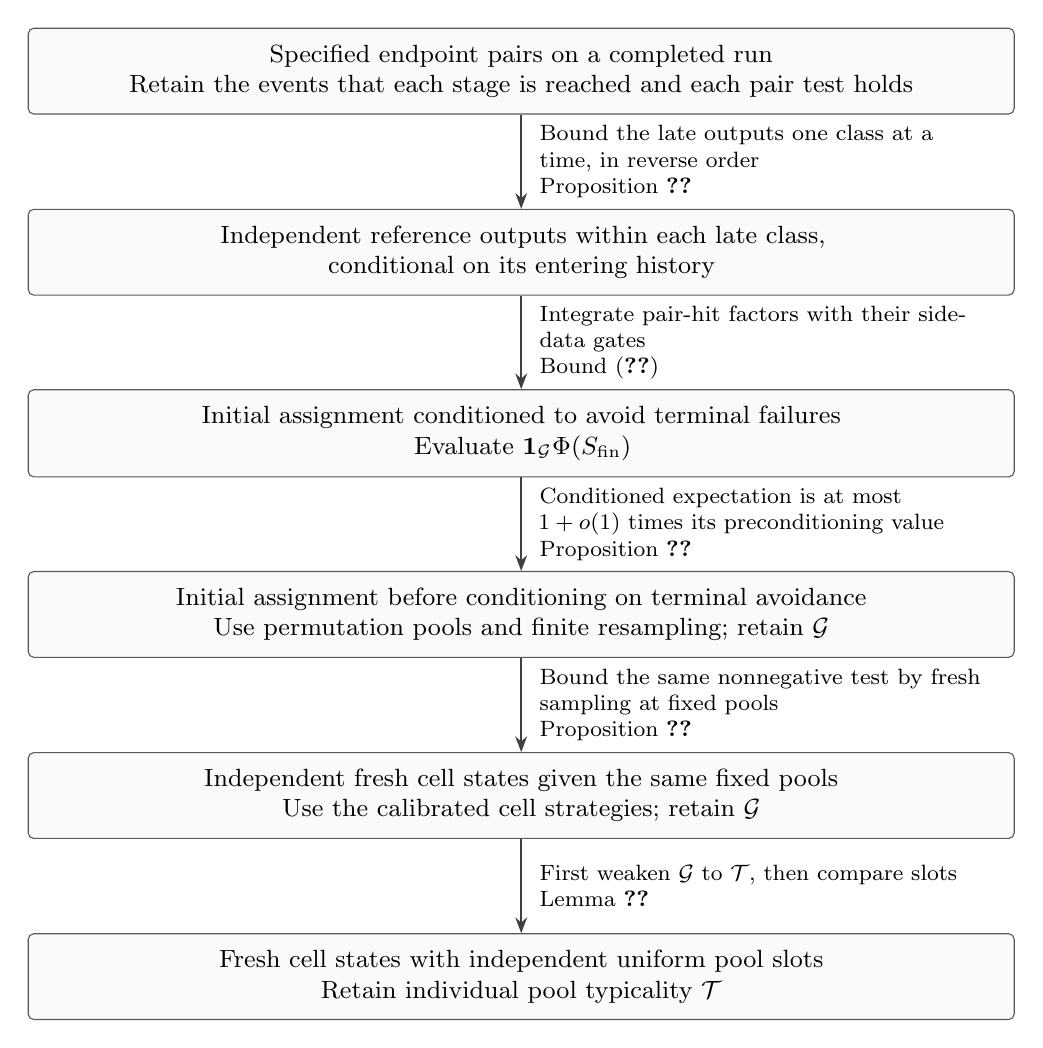
\begin{tikzpicture}[
  box/.style={draw=black!65,rounded corners=2pt,fill=black!2,
    align=center,font=\small,inner sep=6pt,text width=12.1cm,
    minimum height=1.05cm},
  arrow/.style={-{Stealth[length=2mm]},line width=.65pt,draw=black!75},
  note/.style={font=\footnotesize,align=left,text width=5.6cm}
]
\node[box] (actual) at (0,0)
  {Specified endpoint pairs on a completed run\\
   Retain the events that each stage is reached and each pair test holds};
\node[box] (late) at (0,-2.3)
  {Independent reference outputs within each late class,\\
   conditional on its entering history};
\node[box] (lists) at (0,-4.6)
  {Initial assignment conditioned to avoid terminal failures\\
   Evaluate \(\mathbf1_{\mathcal G}\Phi(S_{\rm fin})\)};
\node[box] (initial) at (0,-6.9)
  {Initial assignment before conditioning on terminal avoidance\\
   Use permutation pools and finite resampling; retain \(\mathcal G\)};
\node[box] (fresh) at (0,-9.2)
  {Independent fresh cell states given the same fixed pools\\
   Use the calibrated cell strategies; retain \(\mathcal G\)};
\node[box] (iid) at (0,-11.5)
  {Fresh cell states with independent uniform pool slots\\
   Retain individual pool typicality \(\mathcal T\)};

\draw[arrow] (actual) -- (late)
  node[midway,right=3pt,note]
  {Bound the late outputs one class at a time, in reverse order\\
   Proposition~\ref{prop:late-assignment}};
\draw[arrow] (late) -- (lists)
  node[midway,right=3pt,note]
  {Integrate pair-hit factors with their side-data gates\\
   Bound~\eqref{eq:source-27}};
\draw[arrow] (lists) -- (initial)
  node[midway,right=3pt,note]
  {Conditioned expectation is at most\\
   \(1+o(1)\) times its preconditioning value\\
   Proposition~\ref{prop:terminal-avoidance}};
\draw[arrow] (initial) -- (fresh)
  node[midway,right=3pt,note]
  {Bound the same nonnegative test by fresh sampling at fixed pools\\
   Proposition~\ref{prop:initial-resampling-comparison}};
\draw[arrow] (fresh) -- (iid)
  node[midway,right=3pt,note]
  {First weaken \(\mathcal G\) to \(\mathcal T\), then compare slots\\
   Lemma~\ref{lem:late-classes-cells}};
\end{tikzpicture}
\caption{Upper comparisons for the endpoint product in
Proposition~\ref{prop:low-endpoint-kernels}.
The first two operations alternate, one class at a time in reverse order.
The late comparisons are conditional at each class, with the entering
history indicator retained until that comparison; each pair side-data
gate remains until its hit factor is integrated.
The pool gate \(\mathcal G\) includes individual typicality and
\eqref{eq:source-23} throughout the fixed deterministic simulation
horizons. It is retained through the fixed-pool resampling comparison,
then weakened to individual typicality \(\mathcal T\) before the slot
comparison. Every arrow bounds the indicated nonnegative test; none
asserts equality of laws or independence after avoidance.
The diagram stops before the later within-cell label, bin, pool and
history comparisons for nonisolated rows.}
\label{fig:endpoint-comparisons}
\end{figure}



\begin{proof}\leavevmode\par
\noindent
Figure~\ref{fig:endpoint-comparisons} records the comparison order for the initial-list reduction below.

\paragraph{Late factors and their side-data gates.}
Write \(a_v\ge1/(4\chi_i)\) for the initial palette mass and
\(m_{v,s}\ge.5-3e_{v,s}\) for each subsequent true hit mass.
On a full run the final row is
\[
 q_v(x)=\frac{\mathbf1_{\rm palette}(x)U_v^0(x)}{a_v}
       \prod_{s:\,v\sim b_s}\frac{I_x(y_{b_s})}{m_{v,s}}.
\]
Pair normalization costs at most two, and the squared hit denominators
cost \(4\exp(O(e_{v,s}))\) per late incidence. Summable errors
therefore bound the conditional product of specified pair weights by
\(K^{t'}\Phi(S_{\rm fin})\) times
\(\prod_{v\sim b_s}4I_{x_v}(y_{b_s})I_{z_v}(y_{b_s})\).

At a late role shared by several tested rows, retain one pair hit by
a rule fixed from the position tuple and replace the other factors
by four. Two distinct even roles have at most two common neighbors;
inside geometric components this removes \(O(t'j)\) incidences.
For each retained pair keep the side-data predicate certifying
\eqref{eq:source-27}. It reads the entering history, mask and sketches,
not the current label.

Integrate backwards by class. Keep that class's reach and incoming
bounds until applying its conditional sampler comparison at factor
two. The side-data predicate remains while the corresponding reference
label is integrated, so each retained factor \(4I_xI_z\) has
integral at most \(\exp(O(l e_{v,s}))\). Only then remove its
predicate. The product of these costs is \(K^{t'}\), since each row
has at most one incidence in each class and
\(\max(1,h_i)\sum_s e_{v,s}=O(1)\). The stage comparisons contribute
\(2^r=e^{O(r)}\), and removed incidences contribute \(e^{O(t'j)}\).
What remains is exactly the nonnegative initial test \(\Phi\)
defined above, with none of the late side-data gates left in it.

\paragraph{Terminal and resampling comparisons.}
Retain \(\mathcal G\) while comparing terminal-conditioned initial
sampling to the unconditioned process. Conditional on these pools,
Proposition~\ref{prop:initial-resampling-comparison} applies jointly
to the nonnegative test \(\Phi\) on \(C_*\), replacing final states
by independent fresh states at factor \(1+o(1)\). Only after this
fixed-pool comparison weaken \(\mathcal G\) to \(\mathcal T\) and
replace consulted permutation slots by iid slots.

Write \(\mathbb E_{\rm term}\) for terminal-conditioned initial
sampling, \(\mathbb E_{\rm perm}\) for the original process with
permutation pools and finite resampling, and
\(\mathbb E_{\rm fresh}(\,\cdot\mid\mathcal P)\) for independent
fresh states on fixed pools. The zero convention in the definition
of \(\Phi\) makes it a nonnegative test on all configurations.
These comparisons give
\[
\begin{aligned}
\mathbb E_{\rm term}\!\left[\mathbf1_{\mathcal G}\Phi(S_{\rm fin})\right]
&\le (1+o(1))\,
 \mathbb E_{\rm perm}\!\left[\mathbf1_{\mathcal G}\Phi(S_{\rm fin})\right]\\
&\le (1+o(1))\,
 \mathbb E_{\rm perm}\!\left[\mathbf1_{\mathcal G}
       \mathbb E_{\rm fresh}(\Phi\mid\mathcal P)\right]\\
&\le (1+o(1))\,
 \mathbb E_{\rm iid}\!\left[\mathbf1_{\mathcal T}
       \mathbb E_{\rm fresh}(\Phi\mid\mathcal P)\right],
\end{aligned}
\]
where the last expectation uses independent uniform slots, and each \(1+o(1)\) may absorb the preceding initial-comparison factors. The fixed-pool comparison is applied before weakening \(\mathcal G\) to \(\mathcal T\). The endpoint probability with full-run indicator is bounded by \(\exp(O(r)+O(t'j))K^{t'}\) times the left side, including the cost of omitted shared late incidences in the backward integration above.

\paragraph{Isolated rows.}
After the three displayed comparisons, discard typicality conditions
on pools outside \(C_*\). The direct cells of an isolated row are
disjoint from every other row's cells, so their iid-pool fresh
expectation factors. An upper pair weight is
\[
 H_v(x,z)=\chi_i^2 A_v(x,z)\,
 \mathbb E_{\rm iid,fresh}\!\left[
 \mathbf1_{\mathcal T_v}\sigma_v(x)\sigma_v(z)
 \prod_{b\in B_v^e}
       \frac{I_x(y_b)I_z(y_b)}{D_{i(b)}(x)D_{i(b)}(z)}\right],
\]
where \(\mathcal T_v\) requires typicality of the direct pools,
and invalid internal-prior contributions are zero. We have removed
the initial mass, masked-support and palette-retention gates and the
redundant positive-support indicator from the row factor of \(\Phi\).
Every removal increases the integral.

The external observation cells are distinct and separate from the
own cell. Their fresh singleton comparisons give
\((1+O(n^{-3}))\pi_{i(b)}\) after integration. Then
\eqref{eq:source-24} and Lemma~\ref{lem:fresh-internal-prior} give
\[
 \sum_z H_v(x,z)
 \le K\chi_i\,\mathbb E[\mathbf1_{\rm typ}\sigma_v(x)]
 \le K\chi_i/M_i=K/M.
\]
For the entrywise bound, each prior atom is at most
\(M_i^{-1}e^{O(\log n)}\); crossing factors contribute
\(e^{O(\log n)}\), and the nonconflict cutoff and degrees bound
bulk pair-hit ratios by \(1+O(\xi+\log n/n)\). Hence
\(H_v\le M^{-2}\exp(O(\log n)+O(\xi n))\le M^{-2}e^{.01n}\)
by the prior choice of \(\xi\).

\paragraph{Reducing nonisolates to pair-hit queries.}
For each of the other \(m\) rows first use, on \(J_v\), the cap
\(\sigma_v\le c_i:=M_i^{-1}e^{O(\log n)}\). In particular
\[
 \mathbf1_{J_v}\mathbf1_{\{x,z\in\mathcal D_v^0\}}
                   \sigma_v(x)\sigma_v(z)\le c_i^2.
\]
After this inequality remove all remaining state-dependent
initial-validity, support, mass and palette-retention indicators for
that row. Keep only the deterministic endpoint predicate \(A_v\).
Bound crossing denominators on the envelope and discard their hits.
Bulk pair denominators cost \(4(1+O(\log n/n))\) each. The remaining
random factors are pair-hit indicators of external early bulk labels.
There are no residual tests of the removed own priors.

Index such a query by its even row, observed odd role, outer word,
observed slice, cell and group. At each observed slice choose one even
outer-word family to retain, by a rule depending only on the positions.
Discard the other hit incidences there. Two different outer words have
at most two common one-flip words, and a row has at most one observation
in a fixed slice. Charging to pairs of rows within the geometric
components removes \(O(t'j)\) hits. Let \(k\le mn\) be the number
of retained queries.

Queries in the same slice now arise from one even outer word. Their
internal words have the same palette color and are distinct, so their
distances exceed \(500\rho h_i\). In cluster mode two members of
one projected group differ in at most two internal bits, whereas the
fixed threshold ensures \(500\rho h_i>2\). Thus these groups are
distinct. Their raw primitive consultation radii are at most
\(10\rho h_i\), so those consultations are disjoint as well. When
\(h_i=0\) there is no sharing. This independence will be used only
after removing slice conditioning below.

\paragraph{Repeated bins and reverse summation.}
Apart from deterministic factors, the integral to bound is now
\[
 \mathbb E_{\rm iid,fresh}
       \left[\mathbf1_{\mathcal T_{\rm qry}}\prod_{a=1}^k f_a(Y_a)\right],
 \qquad f_a(y)=I_{x_{v(a)}}(y)I_{z_{v(a)}}(y),
\]
where \(\mathcal T_{\rm qry}\) requires typical pools for the
queried odd cells. Conditional on these pools and their successful
\(W\), let \(D_a\) be the bin chosen for group \(g_a\), and set
\[
 u_a^W(D)=\int f_a\,dU_{g_a}^W(D),\qquad
 J(D)=\{a:D_a=D_b\text{ for some }b<a\text{ in the same cell}\}.
\]
For fixed bin values discard \(f_a\le1\) whenever \(a\in J(D)\).
The remaining queries use at most one label per bin in each cell, so
the conditional label comparison costs \(e^{d_i^{-.01}k}\).
Next the group-bin comparison, applied to all \(k\) distinct group
queries, costs \(e^{d_i^{-.05}k}\). In direct mode bins are singleton
labels; its calibrated cell sampler gives the corresponding upper
comparison at \(e^{o(1)k}\), since \(k\le n^2\).

For a fixed repeat mask \(J\), the sum after these comparisons is
bounded by the appropriate calibration factor times
\[
 \sum_{D_1,\ldots,D_k}\mathbf1_{\{J(D)=J\}}
          \prod_{a=1}^k\widetilde q_{g_a}(D_a)
          \prod_{a\notin J}u_a^W(D_a).
\]
Enlarge the repeat indicator by retaining only distinctness of the
kept targets within each cell and the necessary earlier-bin equality
for each removed query. Sum removed bins in decreasing index order.
At the summation for \(a\in J\), all earlier candidate bins are
still fixed, even if they will be removed later, so
\[
 \sum_{D_a\in\{D_b:b<a\text{ in the same cell}\}}
                   \widetilde q_{g_a}(D_a)
 \le k\|\widetilde q_{g_a}\|_\infty\le n^{-A_c+3}.
\]
No kept factor \(u_a^W(D_a)\) reads a removed bin. This is why the
initial indicators were discarded before the two sampler comparisons.
The total repeat cost is \((n^{-A_c+3})^{|J|}\); kept-bin
distinctness still remains for the pool integral.

\paragraph{Removing pool restrictions and counting the losses.}
On typical pools the kept restricted bin probabilities satisfy
\[
 \widetilde q_g(D)\le
 (1+\varepsilon)(B_i/L_i^{\rm slot})q_g^W(D)
                     \mathbf1_{\{D\in\mathcal P\}},
 \qquad \varepsilon=10^{-5}.
\]
Here \(q_g^W\) is the raw bin law, uniform before trims in direct
mode; the bound includes both trim losses. Undo the \(W\)-cell
load conditioning, at negligible logarithmic cost per query, while
its typical-pool hypothesis is still retained. Then discard the
remaining pool tests. The slice-conditioned \(W\)'s are now
independent of the iid pools. For \(a\) distinct kept targets in
one cell, their simultaneous presence costs at most
\[
 (L_i^{\rm slot})_a/B_i^a\le(L_i^{\rm slot}/B_i)^a.
\]
This cancels the pool-restriction factors. Discard kept-target
distinctness and sum their raw bin kernels. Finally remove the
\eqref{eq:source-15} slice conditioning at cost at most another
\((1+\varepsilon)^k\). Raw primitive inputs are now independent
between slices and between the separated consultations within them.

Their pair-hit means use \(\pi_i^0\) in cluster mode, and are at
most \((1+10^{-4})/4\), by the degree bounds, the pair cutoff and
the total-variation estimate following \eqref{eq:source-16}.
Let \(\delta_{\rm cal}\) include the two per-query calibration
logarithms and the load-normalizer logarithm. With \(\xi\) already
fixed small, increase the fixed threshold \(Q_0\) so that
\[
 \delta_{\rm cal}+2\log(1+\varepsilon)
       +\log(1+10^{-4}+4n^{-A_c+3})\le .005
\]
eventually. This makes the fixed low-cluster errors small; it does
not assume they tend to zero with \(n\). Summing all repeat masks
therefore bounds the \(k\) pair hits by
\[
 e^{(\delta_{\rm cal}+2\log(1+\varepsilon))k}
       \big((1+10^{-4})/4+n^{-A_c+3}\big)^k
 \le4^{-k}e^{.005k}.
\]
For \(k=0\) the bound is one. Each retained pair hit contributes
its factor \(1/4\), cancelling a bulk denominator factor four.
Discarded hits leave \(e^{O(t'j)}\); the prior caps, crossing
factors and degree drift leave \(e^{O(m\log n)}\). Since
\(k\le mn\), the total is at most
\(M_i^{-2m}\exp(.01nm+O(t'j))\). The palette factor
\(\chi_i^{2m}\) turns this into \(M^{-2m}\) with the asserted
error. Together with the isolate weights and the preceding late and
initial comparisons, this proves \eqref{eq:source-28}.
\end{proof}

\begin{lemma}[Two-endpoint Hall estimate]\label{lem:low-two-endpoint-hall}
Assume that the full run has probability \(1-o(1)\), as supplied by
Proposition~\ref{prop:late-assignment}. The joint endpoint bounds of
Proposition~\ref{prop:low-endpoint-kernels}, with the stated palette sizes
and geometric partner counts, then imply simultaneous Hall matchings in
every low-mode palette with positive probability of full success.
\end{lemma}

\begin{proof}\leavevmode\par
\paragraph{Geometric averaging.}
Choose a small constant \(\eta>0\) with
\(.02+C'\eta<(\log2)/2\), and put \(t_0=\lfloor\eta n\rfloor\).
For a uniformly chosen distinct \(p\)-set of positions, \(p\le t_0\),
a geometric overlap graph of rank \(j\) contains a forest of \(j\)
necessary partner relations. Specifying its edges costs at most
\(p^{2j}\); exposing along that forest uses the partner fraction
\(2^{-n+o(n)}\) once per edge. Since \(m\le2j\), the correction in
\eqref{eq:source-28} is at most
\(e^{(.02+C'\eta)nj}\). Its average is bounded by a convergent
geometric sum with ratio \(e^{-(\log2)n/2+o(n)}\).

\paragraph{The endpoint multigraph.}
This graph is different from the geometric overlap graph: its vertices
are host labels, and each even row is an edge joining its two chosen
endpoints. Hall fails precisely when some set of row edges has fewer
incident endpoint vertices than edges. Such a set has a connected
violating component. The actual distinct-endpoint condition is retained
in the following sums, even for nonisolates whose convenient upper
weight \(H_v=M^{-2}\) is positive on the diagonal.

Connectivity of \(p\) distinct row edges is witnessed by a tree on
those rows, with one endpoint identification along each tree link.
There are at most \(4^{p-1}p^{p-1}\) such diagrams. These identifications
leave \(p+1\) abstract endpoint variables, and the row edges form a
tree on them. Summing a product of the row weights by successively
integrating leaves costs at most \(2M(K/M)^p\), using the row-sum
bound and at most \(2M\) choices for the last variable.

A connected Hall-violating \(p\)-set, \(p\ge3\), uses fewer than
\(p\) endpoint vertices. Thus at least two further mergers of distinct
current endpoint classes occur, with \(O(p^4)\) choices. Keep just
these two mergers and discard any additional identifications for an
upper bound. The resulting quotient has \(p-1\) vertices and \(p\)
row edges. On the retained distinct-endpoint support it has no loops;
parallel edges are allowed. A spanning tree uses \(p-2\) edges,
leaving exactly two edges to which the maximum-weight bound applies.
The corresponding sum is at most
\[
 \underbrace{2M}_{\text{root choices}}\,
 \underbrace{(K/M)^{p-2}}_{\text{tree edges}}\,
 \underbrace{(M^{-2}e^{.01n})^2}_{\text{two remaining edges}}
 \le K^pM^{-p-1}e^{.02n}.
\]
The mergers here are independent identifications of equivalence classes,
not probabilistically independent events. Different rows may use
different kernels; the same two uniform bounds suffice.

\paragraph{Summing obstructions.}
Equation~\eqref{eq:source-28}, geometric averaging and
\(\binom Lp\le L^p/p!\) bound the expected number, with full-run
indicator, of connected \(t_0\)-row sets by
\(e^{O(r)}M(K/C_n)^{t_0}\). For smaller connected \(p\)-row sets
with fewer than \(p\) endpoints the bound is
\[
 e^{O(r)}p^4M^{-1}e^{.02n}(K/C_n)^p.
\]
Sizes one and two cannot violate Hall because each row has distinct
endpoints. For the large-set estimate,
\[
 \log\big(M(K/C_n)^{t_0}\big)
 =n\log2+o(n)+\eta n\log(K/C_n)+O(\log n),
\]
which is eventually negative at a linear rate, however slowly
\(C_n\to\infty\). For the small-set sum,
\(M^{-1}e^{.02n}=e^{-(\log2-.02)n+o(n)}\), and
\(\sum_{p\ge3}p^4(K/C_n)^p\) is bounded. Both estimates still tend
to zero after summing over the \(e^{o(n)}\) patches and palettes.

Every connected component with at least \(t_0\) row edges contains
a connected \(t_0\)-row set. Every Hall failure contains a connected
violating component. Consequently the probability of a full run with
no Hall obstruction is at least its probability \(1-o(1)\) minus
the preceding expected obstruction counts, and is positive. Hall gives
distinct representatives simultaneously in all palettes. Palettes
and patches are disjoint, so these choices combine. The early odd
labels are already injective, and the disjoint injective late pools
replace their dummy labels. Every required edge is present, yielding
the monochromatic cube and excluding the low modes.
\end{proof}

\paragraph{Conclusion of Theorem~\ref{thm:main}.}
An unbounded ratio \(R(Q_n)/2^n\) would supply the sequence of
Lemma~\ref{lem:counterexample-sequence}. The earlier exclusions reduce
it to deep discrepancy in both orientations. Patch extraction then
leaves high or low modes. Section~\ref{sec:high-modes-of-the-tiling}
excludes the high modes, and the preceding matching excludes the low
modes. No such sequence exists. The ratio therefore has finite
supremum, giving an absolute \(C\) with \(R(Q_n)\le C2^n\) for all
\(n\). This existence argument does not provide a numerical value
for \(C\).


\clearpage
\appendix
\section{Quantitative guide to the regimes}
\label{app:regime-table}

Table~\ref{tab:all-regimes} records the cases of the proof in their logical
order. All discrepancy and eventual-absence conclusions concern the
retained sides of the stabilized counterexample subsequence, after the
total $o(N)$ label removals specified in the proof, and hold eventually
along that subsequence. Width always means $\log(N\max\mu)$, using
the original host-side size $N$. Thus a normalized atom bound $N\max\mu\le n^D$ gives width
$D\log n$. Defect means density of the other color. Availability means
that, for some fixed $\kappa>0$, a witness can be chosen after every
removal of at most $\kappa N$ labels from each side; the witness may
depend on the removed sets. See
Section~\ref{sec:general-conventions-and-probabilistic-tools}.
Every constant and exponent is fixed before $n\to\infty$, with the
local meaning assigned in its cited section. In particular, parameters
with the same name in different rows need not have the same value.

For the atom bounds below, $p_b$ denotes an odd probability row and $p_v$
an even probability row. A tuple posterior $\Pi_v$ is a law on $k$
first-side labels, so $N^k\max\Pi_v$ is its density bound relative to
the uniform product law. This differs from the one-label bound
$N\max p_v$. The limiting exponents $H^\dagger,H_L^\dagger$ are those
of Definition~\ref{def:limiting-bias-exponents}; they delimit the
available-bias ranges at power and linear width budgets.

The last six rows use initial discrepancy~\eqref{eq:source-2}, deep
discrepancy~\eqref{eq:source-9} in both orientations, and the eventual
cluster-witness absence of Corollary~\ref{cor:eventual-cluster-absence}.
Here $g,q$ are the residual bias and cluster scales of
Definition~\ref{def:residual-scales}; $M_i$ is the size of either side of
patch $i$, $\ell_i$ its prefix length, $h_i$ its internal dimension,
$d_i$ its bin size, and $s_i$ its gain parameter. The cleaned first-side
degrees are measured by
$D_{\pi_i}(x)=\sum_y\pi_i(y)\mathbf1_G(x,y)$, where $\pi_i$ is
uniform on $Y_i$ in the bounded and direct branches and is the comparison
law of Section~\ref{sec:internal-solver-and-profiles-for-these-tilings}
in the cluster branches. Every nonbounded row is reached only after
$\max(g,q)\ge M_1Q_0$. For such a patch the common allocation budget is
\[
 \ell_i,\ \log(N/M_i)\le s_i/(1000u),
\]
where $u$ is the fixed even moment order from
Section~\ref{sec:the-two-deep-orientations-some-estimates}. The word
\emph{bounded} names the first extraction branch; it does not assert that
the scales in every other branch tend to infinity.

\begingroup
\small
\setlength{\tabcolsep}{4pt}
\renewcommand{\arraystretch}{1.18}
\begin{longtable}{@{}>{\raggedright\arraybackslash}p{.255\linewidth}>{\raggedright\arraybackslash}p{.355\linewidth}>{\raggedright\arraybackslash}p{.345\linewidth}@{}}
\caption{All regimes: hypotheses, quantitative costs, and the interface
used by the next stage. In the first reductions an available witness
produces a cube; its exclusion supplies the stated discrepancy or
structural conclusion.}\label{tab:all-regimes}\\
\toprule
Regime and input & Width, density, and loss budget & Output and location\\
\midrule
\endfirsthead
\multicolumn{3}{l}{\textit{Table~\thetable\ continued}}\\
\toprule
Regime and input & Width, density, and loss budget & Output and location\\
\midrule
\endhead
\midrule
\multicolumn{3}{r}{\textit{Continued on the next page}}\\
\endfoot
\bottomrule
\endlastfoot

Counterexample sequence &
$n\to\infty$, $C_n=N/2^n\to\infty$, $N\le n2^n$. No rate is imposed
on $C_n$. &
The bipartite contradiction setting;
Lemma~\ref{lem:counterexample-sequence}.\\

Power-width bias versus purity &
Widths $(n^\beta,n^\gamma)$, $0<\beta\le\gamma<1$; an available
patch with absolute bias $\ge n^{-h}$, and no pair of laws on the
current sets with defect $\le e^{-n^h}$ in either color at the
respective doubled widths $(2n^\beta,2n^\gamma)$.
Here $\omega=\min(\beta,1-\gamma)/1000$, $h=\omega/10^6$.
Filter widths fit the plateau margin;
$N\max p_v\le\exp((\log2-c n^{-h})n)$. &
The two hypotheses together give a cube. The density gain pays for local
repetitions and predictive tests;
Lemma~\ref{lem:bias-purity}.\\

Constant broad side &
Balanced first laws of width $n^\gamma$, $0<\gamma<1$; at least $\chi N$
columns of degree $\ge.95$ for each tag. Given the parents, the stream
law relative to $R[u]$ is $\le e^{a_0u}$, $a_0=1/3$.
The posterior satisfies $N^k\max\Pi_v\le e^{\tau_0kn}$, and
$N\max p_v\le O(e^{\tau_1n})$, with
$a_0<\tau_0<\tau_1<\log2$. &
A cube in that color. The remaining gap below $\log2$ pays for geometric
overlap; Lemma~\ref{lem:constant-broad-high-neighborhood}.\\

Polynomial broad-side concentration and polynomial defect &
Balanced laws of widths at most $n^\gamma$ and $D_*\log n$, $0<\gamma<1$;
every broad-side degree is $\ge1-n^{-p_0}$, for fixed $p_0>0$.
After marginalizing the tag, $N^k\max\Pi_v\le e^{.4kn}$;
$N\max p_v\le O(e^{.55n})$. The constant $D_*>0$ is universal. &
A cube in one of the colors;
Lemma~\ref{lem:small-polynomial-broad-side}. This excludes the sparse
rectangles tested in~\eqref{eq:source-1}.\\

Small-grid purity &
Available patches have both widths $\le n^{d/2}$ and every second-support
degree $\ge1-e^{-n^p}$, $p>0$. Every law pair of widths
$(D_0\log n,n^{1/4})$ has both color densities $>n^{-c}$, where
$0<D_0<\min(.1,D_*/2)$.
Use $d<D_0/1000$, $b=d/4$, $c=b/20$;
$\log(N\max p_b)\le n^{d/2}+2cn^d\log n+O(\log n)$ and
$\log(N\max p_v)\le .04n^{4d}+o(n^{4d})$. &
Purity gives a cube. Together with the power-width alternative this yields
discrepancy $n^{-\eta_0}$ at both widths $n^{\eta_0}$, for a fixed
$\eta_0>0$; Lemma~\ref{lem:small-grid-purity} and
Corollary~\ref{cor:initial-discrepancy}.\\

Asymmetric purity &
Under initial discrepancy~\eqref{eq:source-2}, a finite balanced
mixture has widths $(n^\gamma,n^\beta)$, $\gamma<1$, $0<\beta<\tau/4$, where $\tau=\min(\eta_0/2,.04)/4$;
every second-support degree is $\ge1-e^{-n^p}$ for fixed $p>0$.
With $s=\lceil n^\tau\rceil$, $N\max p_b\le e^{.02s\log n}$
and $N\max p_v\le e^{.1n}$.
No relation $p>\tau$ is required. &
Purity gives a cube. Consequently, at every admissible fixed rational
width pair, all weighted densities differ from $1/2$ by at most a fixed
negative power of $n$, in both orientations;
Lemma~\ref{lem:asymmetric-purity} and
Corollary~\ref{cor:asymmetric-discrepancy}.\\

Intermediate sublinear bias: some $H^\dagger<1$ &
Shallow widths $(n^{x_s},n^{y_s})$ and deep widths
$(n^{x_d},n^{y_d})$, $y_s<1-\sigma<y_d$.
Available bias $2a_*=n^{-h_+}$; deep error $b_*=n^{-h_-}$,
$0<h_-<h_+<1$, $h_+-h_-<\chi/10$.
The gain $cna_*$ pays for first-side width and
$O(n^\sigma\log n)$ local entropy. &
A cube, using a core of size $\le n^\chi$ and an outside-core read bound
$n^\sigma+3$; Proposition~\ref{prop:intermediate-bias-exclusion}.
This excludes the whole range $H^\dagger<1$, including zero.\\

Intermediate linear bias: both $H^\dagger\ge1$, some
$0<H_L^\dagger<1$ &
Shallow widths $(n^{x_s},\alpha_s n)$ and deep widths
$(n^{x_d},\alpha_d n)$, $100\alpha_s<\alpha_d$.
Use $a_*=\tfrac12n^{-h_+}$, $b_*=n^{-h_-}$ with parameters chosen
afresh in the linear case; $\sigma<\chi/10$ and broad-test error
$o(a_*)$. The read-tail exponent is
$na_*^2/((n^\sigma+3)b_*^2)$. &
A cube. The surplus survives the external-coordinate costs;
Proposition~\ref{prop:intermediate-bias-exclusion}.
The two intermediate cases use different parameter orders.\\

Full-dimensional clusters &
Assume initial discrepancy in both orientations and available one-color
patches. The first law and aggregate second law have widths
$\le n^\delta$; individual cluster atoms are $\le e^{-n^\zeta}$.
Codegrees, including repeated labels, are $\ge1/4+n^{-\delta}$.
Here $\delta<\min(\eta_0,\zeta,1)/2000$ and
$k(T+m)=O(n^{500\delta})$ fits both discrepancy and atom budgets.
The even bound is $N\max p_v\le e^{(\log2-.01n^{-\delta})n}$. &
A cube, hence eventual absence for every fixed admissible rational
choice. Used in the linear jump and again in extraction;
Proposition~\ref{prop:full-dimensional-cluster-exclusion} and
Corollary~\ref{cor:eventual-cluster-absence}.\\

Linear-budget jump: both $H^\dagger\ge1$, some $H_L^\dagger=0$ &
Available widths $(n^{.01},.011n)$ with column surplus $2n^{-.01}$.
Reverse-orientation discrepancy $n^{-.95}$ at widths
$(n^{1-\upsilon/4},n^{x_0})$.
The internal dimension $n^{.1}$ gives gain $n^{.09}$, exceeding
$O(n^{.05})+n^{.03}$ losses. &
A cube; Proposition~\ref{prop:linear-budget-jump-exclusion}.
Thus both $H_L^\dagger\ge1$ remain.\\

Deep discrepancy &
Widths $(\alpha n,n^{x_*})$ in either order, for fixed
$0<\alpha,x_*<.01$; error $b_*=n^{-1+.04}$.
Every fixed smaller positive error slack is available with possibly
smaller budgets. The interaction tails use the setting of
Lemma~\ref{lem:heterogeneous-centered-moment}: the first law $\tau$
and second laws $\pi_l$ have widths $\le n^{x_*/4}$, with
$|D_{\pi_l}(x)-1/2|\le O(b_*)$ on $\operatorname{supp}\tau$.
For each fixed $u$, the one-free threshold $O_u(b_*)$ has tail
$e^{-\alpha n/3}$, and the two-free threshold $n^{-1-.03}$ has tail
$e^{-n^{.4}}$. &
Interaction moments, row trimming, and homogeneous clique peeling;
Corollary~\ref{cor:deep-discrepancy} and
Lemmas~\ref{lem:deep-interaction-tails}--\ref{lem:simultaneous-row-trimming}.
Interaction bounds allow different laws at different coordinates;
clique peeling uses a single common law.\\

Bounded extraction: $\max(g,q)<M_1Q_0$ &
One patch $M_i\asymp N$, $\ell_i=h_i=s_i=0$.
On cleaned supports, $|D_{\pi_i}(x)-1/2|\le K/n$ and the number
of labels with a large interaction is bounded by a fixed constant.
The $r\asymp A_0\log n$ late classes supply polynomial slack. &
Two surviving candidates per even role, with joint bounds that give Hall;
Proposition~\ref{prop:patch-extraction-allocation},
Lemma~\ref{lem:stable-patch-cleaning}, and
Sections~\ref{sec:low-modes-geometry-and-cell-states}--\ref{sec:late-dynamics-and-its-transfer-problem}.\\

Low direct: $g>M_1q$, $g\le K_B\log n$ &
$M_i\ge cNe^{-g^{a_B}}$, $h_i=0$, $s_i=10^{-3}g$.
On cleaned supports,
$1/2+g/(4n)\le D_{\pi_i}(x)\le1/2+4g/n$.
Prefix and width losses are $\le s_i/(1000u)$; late classes pay for
the remaining list losses. &
Two surviving candidates per even role, with joint bounds that give Hall;
Proposition~\ref{prop:patch-extraction-allocation},
Lemma~\ref{lem:stable-patch-cleaning}, and
Lemma~\ref{lem:low-two-endpoint-hall}.\\

High direct: $g>M_1q$, $g>K_B\log n$ &
The same direct patch budgets and degree interval.
The homogeneous peel parameter is $\le e^{-200s_i}$, giving mass-failure
probability $\le n^{-R}$. The unnormalized row bound
$M_iZ_v(x)\le2^n e^{-200s_i}$ pays for repeated local neighborhoods. &
An odd injection and even weights $Z_v$ supported on common neighbors,
with row masses $\ge1/2$ and column sums $\le1/2$. Normalizing gives Hall;
Lemma~\ref{lem:high-direct-assignment}.\\

Low cluster: $g\le M_1q$, $Q_0\le q\le(\log n)^{c_q}$ &
$M_i\ge cNe^{-q^{a_C}}$, $d_i=\lfloor e^{q/2}\rfloor$,
$q^{M_{\rm lo}}\le h_i<2q^{M_{\rm lo}}$,
$s_i=ah_i/10^6$.
Within-bin codegree is $\ge1/4+a$; on cleaned supports,
$|D_{\pi_i}(x)-1/2|\le10q^{C_b}/n$, with
$10q^{C_b}<s_i/(100u)$. Also $h_i\le(\log n)^{.1}$. &
Exact group and label marginals preserve the mean estimates.
The later assignment gives two candidates per even role and Hall;
Proposition~\ref{prop:internal-slice-solver},
Propositions~\ref{prop:calibrated-group-bins}
and~\ref{prop:calibrated-role-labels},
Lemma~\ref{lem:low-two-endpoint-hall}.
The scales $q,h_i,d_i$ may stay fixed.\\

High cluster with small bins: $g\le M_1q$,
$(\log n)^{c_q}<q\le(\log n)^2$ &
The same cluster width, gain, degree, and codegree bounds, with
$q^{M_{\rm hi}}\le h_i<2q^{M_{\rm hi}}$; $d_i$ is the smaller of
$\lfloor e^{q/2}\rfloor$ and $\lfloor e^{\sqrt{\log n}}\rfloor$.
Here $h_i>(\log n)^5$ and $h_i=o(d_i^{.025})$.
Exact singleton and calibrated joint estimates control repeated bins. &
An odd injection and even weights $Z_v$ with row masses $\ge1/2$
and column sums $\le1/2$. Normalizing the rows gives Hall;
Propositions~\ref{prop:high-cluster-sampling}
and~\ref{prop:high-cluster-loads}.\\

High cluster with large bins: $g\le M_1q$, $q>(\log n)^2$ &
The same cluster budgets, now $d_i=\lfloor e^{q/2}\rfloor$ and
$q^{M_{\rm hi}}\le h_i<2q^{M_{\rm hi}}$.
With $k_i=\lceil h_i^{3\omega}\rceil$,
$T_i=\lceil h_i^\omega\rceil$, all cluster modes have
$k_iT_i\ll q^{a_C/2},\log d_i$.
The conditional in-bin label law satisfies
$\max_y U_g^W(D)(y)\le2e^{1.5k_iT_i}/d_i$, a superpolynomially
small bound. &
An odd injection and even weights $Z_v$ with row masses $\ge1/2$
and column sums $\le1/2$. Normalizing the rows gives Hall;
Propositions~\ref{prop:high-cluster-sampling}
and~\ref{prop:high-cluster-loads}.\\
\end{longtable}
\endgroup

\paragraph{Exhaustion and boundary conventions.}
The intermediate-bias proposition first excludes $H^\dagger<1$ in either
orientation. Once both $H^\dagger\ge1$, each $H_L^\dagger$ belongs to
$\{0\}$, $(0,1)$, or $[1,+\infty]$. The first two possibilities are
excluded separately, and the third gives deep discrepancy by taking
strictly smaller error exponents. No conclusion at the threshold defining
an infimum is needed.

During extraction the bounded case is tested first. Outside it,
$g\le M_1q$ implies $q\ge Q_0$, so the cluster branch is defined.
Equality at $g=M_1q$ belongs to the cluster branch, equality at
$g=K_B\log n$ to low direct, and equality at either cluster threshold
to the lower range. The fixed choice of $Q_0$ makes estimates in its
positive powers uniformly sufficient; it never licenses replacing a
fixed-scale error by an error tending to zero with $n$.

\clearpage
\phantomsection
\addcontentsline{toc}{section}{\refname}
\begin{thebibliography}{99}

\bibitem{azuma1967}
K.~Azuma,
Weighted sums of certain dependent random variables,
\emph{Tohoku Mathematical Journal}
(2) \textbf{19} (1967), no.~3, 357--367.
\url{https://doi.org/10.2748/tmj/1178243286}.

\bibitem{beck1983}
J.~Beck,
An upper bound for diagonal Ramsey numbers,
\emph{Studia Scientiarum Mathematicarum Hungarica}
\textbf{18} (1983), no.~2--4, 401--406.

\bibitem{burr-erdos1975}
S.~A.~Burr and P.~Erd\H{o}s,
On the magnitude of generalized Ramsey numbers for graphs,
in \emph{Infinite and Finite Sets}, Vol.~I (Keszthely, 1973),
Colloquia Mathematica Societatis J\'anos Bolyai \textbf{10},
North-Holland, Amsterdam, 1975, pp.~215--240.
\url{https://www.renyi.hu/~p_erdos/1975-26.pdf}.

\bibitem{chvatal-rodl-szemeredi-trotter1983}
V.~Chv\'atal, V.~R\"odl, E.~Szemer\'edi and W.~T.~Trotter, Jr.,
The Ramsey number of a graph with bounded maximum degree,
\emph{Journal of Combinatorial Theory, Series B}
\textbf{34} (1983), no.~3, 239--243.
\url{https://doi.org/10.1016/0095-8956(83)90037-0}.

\bibitem{conlon2009bipartite}
D.~Conlon,
Hypergraph packing and sparse bipartite Ramsey numbers,
\emph{Combinatorics, Probability and Computing}
\textbf{18} (2009), no.~6, 913--923.
\url{https://doi.org/10.1017/S0963548309990174}.

\bibitem{conlon-fox-lee-sudakov2016}
D.~Conlon, J.~Fox, C.~Lee and B.~Sudakov,
Ramsey numbers of cubes versus cliques,
\emph{Combinatorica} \textbf{36} (2016), 37--70.
\url{https://doi.org/10.1007/s00493-014-3010-x}.

\bibitem{conlon-fox-sudakov2016}
D.~Conlon, J.~Fox and B.~Sudakov,
Short proofs of some extremal results II,
\emph{Journal of Combinatorial Theory, Series B} \textbf{121}
(2016), 173--196.
\url{https://doi.org/10.1016/j.jctb.2016.03.005}.

\bibitem{dirr-dondl-grimmett-holroyd-scheutzow2010}
N.~Dirr, P.~W.~Dondl, G.~R.~Grimmett, A.~E.~Holroyd and M.~Scheutzow,
Lipschitz percolation,
\emph{Electronic Communications in Probability} \textbf{15} (2010), 14--21.
\url{https://doi.org/10.1214/ecp.v15-1521}.

\bibitem{erdos-lovasz1975}
P.~Erd\H{o}s and L.~Lov\'asz,
Problems and results on \(3\)-chromatic hypergraphs and some related questions,
in \emph{Infinite and Finite Sets} (Keszthely, 1973),
Colloquia Mathematica Societatis J\'anos Bolyai \textbf{10} (1975), 609--627.
\url{https://users.renyi.hu/~p_erdos/1975-34.pdf}.

\bibitem{erdos-spencer1991}
P.~Erd\H{o}s and J.~Spencer,
Lopsided Lov\'asz Local Lemma and Latin transversals,
\emph{Discrete Applied Mathematics} \textbf{30} (1991),
nos.~2--3, 151--154.
\url{https://doi.org/10.1016/0166-218X(91)90040-4}.

\bibitem{finner1992}
H.~Finner,
A generalization of H\"older's inequality and some probability inequalities,
\emph{The Annals of Probability} \textbf{20} (1992), no.~4, 1893--1901.
\url{https://doi.org/10.1214/aop/1176989534}.

\bibitem{fiz-pontiveros-griffiths-morris-saxton-skokan2014}
G.~Fiz Pontiveros, S.~Griffiths, R.~Morris, D.~Saxton and J.~Skokan,
The Ramsey number of the clique and the hypercube,
\emph{Journal of the London Mathematical Society}
\textbf{89} (2014), no.~3, 680--702.
\url{https://doi.org/10.1112/jlms/jdu004}.

\bibitem{fiz-pontiveros-griffiths-morris-saxton-skokan2016}
G.~Fiz Pontiveros, S.~Griffiths, R.~Morris, D.~Saxton and J.~Skokan,
On the Ramsey number of the triangle and the cube,
\emph{Combinatorica} \textbf{36} (2016), 71--89.
\url{https://doi.org/10.1007/s00493-015-3089-8}.

\bibitem{fox-sudakov2009}
J.~Fox and B.~Sudakov,
Density theorems for bipartite graphs and related Ramsey-type results,
\emph{Combinatorica} \textbf{29} (2009), no.~2, 153--196.
\url{https://doi.org/10.1007/s00493-009-2475-5}.

\bibitem{freedman1975}
D.~A.~Freedman,
On tail probabilities for martingales,
\emph{The Annals of Probability} \textbf{3} (1975), no.~1, 100--118.
\url{https://doi.org/10.1214/aop/1176996452}.

\bibitem{gandhi-khuller-parthasarathy-srinivasan2006}
R.~Gandhi, S.~Khuller, S.~Parthasarathy and A.~Srinivasan,
Dependent rounding and its applications to approximation algorithms,
\emph{Journal of the ACM} \textbf{53} (2006), no.~3, 324--360.
\url{https://doi.org/10.1145/1147954.1147956}.

\bibitem{gowers1998}
W.~T.~Gowers,
A new proof of Szemer\'edi's theorem for arithmetic progressions of length four,
\emph{Geometric and Functional Analysis} \textbf{8} (1998), no.~3, 529--551.
\url{https://doi.org/10.1007/s000390050065}.

\bibitem{graham-rodl-rucinski2001}
R.~L.~Graham, V.~R\"odl and A.~Ruci\'nski,
On bipartite graphs with linear Ramsey numbers,
\emph{Combinatorica} \textbf{21} (2001), no.~2, 199--209.
\url{https://doi.org/10.1007/s004930100018}.

\bibitem{haeupler-saha-srinivasan2011}
B.~Haeupler, B.~Saha and A.~Srinivasan,
New constructive aspects of the Lov\'asz Local Lemma,
\emph{Journal of the ACM} \textbf{58} (2011), no.~6,
Article~28, 1--28.
\url{https://doi.org/10.1145/2049697.2049702}.

\bibitem{hall1935}
P.~Hall,
On representatives of subsets,
\emph{Journal of the London Mathematical Society}
(1) \textbf{10} (1935), no.~1, 26--30.
\url{https://doi.org/10.1112/jlms/s1-10.37.26}.

\bibitem{hamming1950}
R.~W.~Hamming,
Error detecting and error correcting codes,
\emph{Bell System Technical Journal} \textbf{29} (1950), no.~2, 147--160.
\url{https://doi.org/10.1002/j.1538-7305.1950.tb00463.x}.

\bibitem{harris-srinivasan2017}
D.~G.~Harris and A.~Srinivasan,
Algorithmic and enumerative aspects of the Moser--Tardos distribution,
\emph{ACM Transactions on Algorithms} \textbf{13} (2017), no.~3,
Article~33, 1--40.
\url{https://doi.org/10.1145/3039869}.

\bibitem{hoeffding1963}
W.~Hoeffding,
Probability inequalities for sums of bounded random variables,
\emph{Journal of the American Statistical Association}
\textbf{58} (1963), no.~301, 13--30.
\url{https://doi.org/10.1080/01621459.1963.10500830}.

\bibitem{kakutani1941}
S.~Kakutani,
A generalization of Brouwer's fixed point theorem,
\emph{Duke Mathematical Journal} \textbf{8} (1941), no.~3, 457--459.
\url{https://doi.org/10.1215/S0012-7094-41-00838-4}.

\bibitem{kostochka-rodl2001}
A.~V.~Kostochka and V.~R\"odl,
On graphs with small Ramsey numbers,
\emph{Journal of Graph Theory} \textbf{37} (2001), no.~4, 198--204.
\url{https://doi.org/10.1002/jgt.1014}.

\bibitem{lee2017}
C.~Lee,
Ramsey numbers of degenerate graphs,
\emph{Annals of Mathematics} (2) \textbf{185} (2017), no.~3, 791--829.
\url{https://doi.org/10.4007/annals.2017.185.3.2}.

\bibitem{lu-szekely2007}
L.~Lu and L.~A.~Sz\'ekely,
Using Lov\'asz local lemma in the space of random injections,
\emph{The Electronic Journal of Combinatorics}
\textbf{14} (2007), no.~1, Research Paper~63.
\url{https://doi.org/10.37236/981}.

\bibitem{moser-tardos2010}
R.~A.~Moser and G.~Tardos,
A constructive proof of the general Lov\'asz Local Lemma,
\emph{Journal of the ACM} \textbf{57} (2010), no.~2,
Article~11, 1--15.
\url{https://doi.org/10.1145/1667053.1667060}.

\bibitem{mota-sarkozy-schacht-taraz2015}
G.~O.~Mota, G.~N.~S\'ark\"ozy, M.~Schacht and A.~Taraz,
Ramsey numbers for bipartite graphs with small bandwidth,
\emph{European Journal of Combinatorics} \textbf{48}
(2015), 165--176.
\url{https://doi.org/10.1016/j.ejc.2015.02.018}.

\bibitem{ramsey1930}
F.~P.~Ramsey,
On a problem of formal logic,
\emph{Proceedings of the London Mathematical Society}
(2) \textbf{30} (1930), 264--286.
\url{https://doi.org/10.1112/plms/s2-30.1.264}.

\bibitem{shi2001}
L.~Shi,
Cube Ramsey numbers are polynomial,
\emph{Random Structures \& Algorithms} \textbf{19} (2001), no.~2, 99--101.
\url{https://doi.org/10.1002/rsa.1021}.

\bibitem{shi2007}
L.~Shi,
The tail is cut for Ramsey numbers of cubes,
\emph{Discrete Mathematics} \textbf{307} (2007), no.~2, 290--292.
\url{https://doi.org/10.1016/j.disc.2006.07.005}.

\bibitem{sudakov2003}
B.~Sudakov,
A few remarks on Ramsey--Tur\'an-type problems,
\emph{Journal of Combinatorial Theory, Series B}
\textbf{88} (2003), no.~1, 99--106.
\url{https://doi.org/10.1016/S0095-8956(02)00038-2}.

\bibitem{tikhomirov2024}
K.~Tikhomirov,
A remark on the Ramsey number of the hypercube,
\emph{European Journal of Combinatorics} \textbf{120}
(2024), article 103954.
\url{https://doi.org/10.1016/j.ejc.2024.103954}.
Preprint: \url{https://arxiv.org/abs/2208.14568}.

\end{thebibliography}

\end{document}
